% Created 2018-06-01 Fri 14:47
% Intended LaTeX compiler: pdflatex
\documentclass[12pt]{book}
\usepackage[utf8]{inputenc}

\usepackage[a4paper,titlepage,markboth,pagenumber]{polytechnique}
\renewcommand{\baselinestretch}{1.1}

\usepackage[T1]{fontenc}
\usepackage{graphicx}
\usepackage{grffile}
\usepackage{longtable}
\usepackage{wrapfig}
\usepackage{rotating}
\usepackage[normalem]{ulem}
\usepackage{amsmath}
\usepackage{textcomp}
\usepackage{amssymb}
\usepackage{capt-of}
\usepackage{amsthm}
\usepackage{amsmath,amscd,amssymb,mathtools}
\usepackage{hyperref}
\usepackage{tikz-cd}
\usepackage{svg}
\usepackage[all]{xy}
\usepackage{pgfplots}
\newtheorem{remark}{Remark}
\newtheorem{theorem}{Theorem}
\newtheorem{lemma}[theorem]{Lemma}
\newtheorem{corollary}{Corollary}[theorem]
\newtheorem{conjecture}[theorem]{Conjecture}
\newtheorem{proposition}[theorem]{Proposition}
\newtheorem{problem}{Problem}
\newtheorem{exampl}{Example}
\newtheorem{definition}{Definition}
\newtheorem{propdef}[definition]{Proposition-Definition}
\newtheorem{fact}{Fact}
\newtheorem{assertion}{Assertion}

\newcommand{\re}{\mathop{\rm Re}\nolimits}
\newcommand{\im}{\mathop{\rm Im}\nolimits}
\newcommand{\coker}{\mathop{\rm coker}\nolimits}
\newcommand{\supp}{\mathop{\rm supp}\nolimits}
\newcommand{\ord}{\mathop{\rm ord}\nolimits}
\newcommand{\Spec}{\mathop{\rm Spec}\nolimits}
\newcommand{\vol}{\mathop{\rm vol}\nolimits}
\newcommand*{\transp}[2][-3mu]{\ensuremath{\mskip1mu\prescript{\smash{\mathrm t\mkern#1}}{}{\mathstrut#2}}}
\newcommand{\sff}{\mathop{\rm I\*I}\nolimits}
\newcommand{\tr}{\mathop{\rm Tr}\nolimits}
\newcommand{\const}{\mathop{\rm const }\nolimits}
\newcommand{\lcm}{\mathop{\rm lcm}\nolimits}
%\newcommand{\gcd}{\mathop{\rm gcd}\nolimits}
\newcommand{\Ric}{\mathop{\rm Ric}\nolimits}
\newcommand{\Riem}{\mathop{\rm Riem}\nolimits}
\newcommand\restr[2]{{% we make the whole thing an ordinary symbol
\left.\kern-\nulldelimiterspace % automatically resize the bar with \right
#1 % the function
\vphantom{\big|} % pretend it's a little taller at normal size
\right|_{#2} % this is the delimiter
}}
\author{Tien NGUYEN MANH}
\date{July 3, 2018}
\title{Harmonic maps\\ of Riemannian manifolds}
\subtitle{Supervised by \\Joel FINE}

\hypersetup{
 pdfauthor={Tien NGUYEN MANH},
 pdftitle={Harmonic maps of Riemannian manifolds},
 pdfkeywords={},
 pdfsubject={},
 pdfcreator={Emacs 25.3.1 (Org mode 9.0.5)}, 
 pdflang={English}}
\begin{document}

\maketitle

\section*{Déclaration d’intégrité relative au plagiat}
\label{sec:declaration}
Je soussigné, \textbf{Manh-Tien NGUYEN}, certifie sur l'honneur :

\begin{itemize} 
\item Que les résultats décrits dans ce rapport sont l’aboutissement de mon travail.
\item Que je suis l’auteur de ce rapport.

\item   Que je n’ai pas utilisé des sources ou résultats tiers sans clairement les citer et les référencer selon les règles bibliographiques préconisées.

\end{itemize}
 Je déclare que ce travail ne peut être suspecté de plagiat.

 \vspace{2cm}

\begin{minipage}{0.5\textwidth}
\begin{flushleft}
\emph{Signature:}\\
\href{}{Manh-Tien NGUYEN} 
\end{flushleft}
\end{minipage}
\begin{minipage}{0.5\textwidth}
\begin{flushright}
\emph{Date :} \\
\href{}{03/07/2018} 
\end{flushright}
\end{minipage}\\[3cm]


\newpage

\section*{Acknowledgements}

I sincerely thank Joel Fine for introducing me to the subject, for the references and for his prompt responses to
all of my questions that enlightened me on many details of this memoire.

I also want to thank Bruno Premoselli for reading this master thesis and for his
participation in its defense.


\newpage

\tableofcontents
\chapter{Summary}
\iffalse
\begin{info}
The PDF version of this page can be downloaded by replacing \texttt{html} in the its address by
\texttt{pdf}. 
For example \texttt{/html/sheaf-cohomology.html} should become \texttt{/pdf/sheaf-cohomology.pdf}.
\end{info}
\fi

\iffalse
Here is the \href{../Stage 2018/main.pdf}{memoire}.
\fi

\section{Summary}
\label{sec:org7287a1a}

The goal of this part is to give a summary of what will be developed in the next chapters. In brief, we are interested in
maps \(f: M \longrightarrow M'\) between Riemannian manifolds (that to simplify, are
supposed to be compact) that are critical points of the energy functional
\[
 E(f) = \frac{1}{2}\int_M |\nabla f|^2 dV.
\]
By taking first order variation of \(E\), these are maps whose \textbf{tension field} \(\tau(f)\) vanishes. 


\subsection{Deformation using nonlinear heat equation.}
\label{sec:org9617dcd}

The approach of \cite{eells_harmonic_1964} is to prove that, if the target space is
negatively curved, then any smooth map \(f_0: M \longrightarrow M'\) can be deformed to a
harmonic map using the gradient descent equation:
\begin{equation}
\label{eq:intro:1}
\begin{cases}
\frac{df_t}{dt} = \tau(f_t)\\
\restr{f}{t=0} = f_0
\end{cases}
\end{equation}
We will prove that if \(M'\) is negatively curved then this PDE admits a globally defined smooth
solution \(f_t\) and that \(f_{\infty}:=\lim_{t\to \infty} f_t\) in \(C^\infty\) is
a harmonic map.

The resolution of \eqref{eq:intro:1} can be organised in 3 steps:
\begin{enumerate}
\item Find the global equation. We will find a global frame of \(M'\) and express
\(f\) in this frame, so that instead of solving for a map, we will have to solve for functions.
\item Study linear PDEs on manifolds. The equation, expressed in local coordinates, is a nonlinear heat equation, i.e. other
than a heat operator, it has a quadratic term. Short-time existence and regularity for \eqref{eq:intro:1} follows from \emph{standard} results of
parabolic equation.
\item Prove long-time existence. In order to use continuity method, we will have to prove
that \(W^{k,p}\)-norms of the solution \(f_t\) do not explode. This will be
established first in the case \(W^{2,2}\) using physical quantities, namely the
potential energy \(E\) and the kinetic energy \(K\). The general case is proved
from the \(W^{2,2}\) estimate using Gårding's inequality and Comparison theorem for
parabolic equation.
\end{enumerate}

The hypothesis of negative curvature is only used to establish the energy
estimates. During deformation, the rate of potential energy can be calculated as: 
\[
 \frac{d e(f_t)}{dt}= -\Delta e(f_t) - |\beta(f_t)|^2 - \left\langle \Ric(M) \nabla_v
f_t,\nabla_v f_t \rangle + \langle \Riem(M') (\nabla_v f_t,\nabla_w f_t)\nabla_v
f_t,\nabla_w f_t \right\rangle
\]
and the kinetic energy as:
\[
 \frac{d k(f_t)}{dt}= -\Delta k(f_t) - \left|\nabla \frac{\partial f_t}{\partial t}\right|^2 +
\left\langle \Riem(M') (\nabla_v f_t,\frac{\partial f_t}{\partial t})\nabla_v
f_t,\frac{\partial f_t}{\partial t} \right\rangle
\]
Therefore if all sectional curvatures of \(M'\) are negative, these rates can be
controlled and the energies are guaranteed not to explode.

\subsection{Existence using Morse-Palais-Smale theory.}
\label{sec:orgc4e17a9}
We also give a less detailed review of the work by Sacks and Uhlenbeck
\cite{sacks_existence_1981}. This approach uses an approximating family \(E_\alpha\) of the energy functional \(E\) whose critical functions in \(W^{1,2\alpha}\) can be easily proved
to exist using Morse-Palais-Smale theory. One then tries to prove that the critical sequence
\(C^1\)-converges to a nontrivial limit. 

As a concrete result, the authors proved,
using an extension theorem for harmonic maps on surface and a suitable covering of \(M\) by small discs on which the energy \(E\) is sufficiently small, that if
the fundamental group \(\pi_k(M')\) is nontrivial for a certain \(k\geq 2\), or
equivalently, if the universal covering \(\tilde M'\) of \(M'\) is not contractible,
then there exists a nontrivial harmonic map from \(\mathbb{S}^2\) to \(M'\).


\iffalse
\bibliographystyle{alpha}
\bibliography{../res/Stage2018}
\fi


\part{Harmonic maps: Introduction}
\chapter{Harmonic maps of Riemannian manifolds}
\iffalse
\begin{info}
The PDF version of this page can be downloaded by replacing \texttt{html} in the its address by
\texttt{pdf}. 
For example \texttt{/html/sheaf-cohomology.html} should become \texttt{/pdf/sheaf-cohomology.pdf}.
\end{info}
\fi

\iffalse
This is my reading note for \cite{eells_harmonic_1964}.
\fi

\section{Harmonic maps}
\label{sec:org9145a27}
\subsection{Variational approach: energy integral and tension field}
\label{sec:org81233e1}
\paragraph{Notation.}
\label{sec:org8daaba0}
Let \(M, M', M''\) be Riemannian manifolds of dimension \(n, n'\) and \(n', n''\)
respectively. We will use \(i,j,k,\dots, \alpha,\beta,\gamma,\dots, a,b,c\) for local
coordinates of \(M, M', M''\).
Let \(f: M \longrightarrow M', f': M' \longrightarrow M''\) be a smooth maps, one denotes
\[
f^\alpha_i = \frac{\partial f^\alpha}{\partial x^i},\quad f^\alpha_{ij} =
\frac{\partial^2 f^\alpha}{\partial x^i \partial x^j} - \Gamma_{ij}^k f^{\alpha}_k \]
so that \(\nabla h = h_i dx^i\) and \(\nabla (\nabla h) = h_{ij}dx^i\otimes dx^j\) and
\(-\Delta h = \tr \nabla (\nabla h) = g^{ij}h_{ij}\) for any smooth function \(h\).


\begin{definition}
The \textbf{energy desity} of \(f\) at \(p\in m\) is defined by
\[
e(f)(p) = \frac{1}{2}\langle g, f^*g \rangle_p = \frac{1}{2}g^{ij}f^\alpha_i
f^\beta_j g'_{\alpha\beta}
\]
and the \textbf{energy functional} of \(f\) is
\[
E(f) = \int_M e(f) dV = \frac{1}{2}\int_M g^{ij}f^\alpha_i
f^\beta_j g'_{\alpha\beta} |\det (g_{ij})|^\frac{1}{2} dx^1\wedge \dots\wedge dx^n
\]
\end{definition}

We recall that the inner product is between 2 tensors of type \((p,q)\) \(S =
S^{i_1\dots i_p}_{j_1\dots j_q}, T = T^{k_1\dots k_p}_{l_1\dots l_q}\) is \(\prod_{m,n}
g_{i_m k_m} g^{j_n l_m}S^{i_1\dots i_p}_{j_1\dots j_q} T^{k_1\dots k_p}_{l_1\dots l_q}\)

\begin{remark}
The energy density is non-negative at every point. Hence \(E(f) = 0\) if and only if \(e(f)=0\) at all points if and only if \(f\) is constant.
\end{remark}

\begin{definition}
Let \(\sigma\) be a symmetric function of \(n\) variables and \(\alpha\) be a
symmetric (0,2) tensor field, one can define the \textbf{\(\sigma\)-energy desity} of \(\alpha\) at \(P\in M\) to be \(\sigma
(\beta_1,\dots,\beta_n)(P)\) where \(\beta_i\) are eigenvalues of the linear operator
\((g^{ik}\alpha_{ij})_{k,j}\). The \textbf{\(\sigma\)-energy} of \(\alpha\) is \(I_\sigma(\alpha)
:= \int_M  \sigma(\alpha) dV\)

Take \(\alpha = f^*g'\), one calls \(\sigma(\alpha)\) the \textbf{\(\sigma\)-energy density}
of \(f\) and \(I_\sigma(\alpha)\) the \(\sigma\)-energy of \(f\).
\end{definition}

\begin{exampl}
For example, the energy functional \(E(f)\) is \(I_\frac{\sigma_1}{2}(f)\). \(V(f):=I_{\sigma^{1/2}_n}(f)\) is called the \textbf{volume} of \(f\).
\end{exampl}

\begin{lemma}[variation of the energy]
\label{lem:var-energy}
Let \(f_t: M \longrightarrow M'\) be a smooth family of smooth maps between Riemannian
manifolds for \(t\in (t_0,t_1)\). Then
\[
\frac{d}{dt}E(f_t) = -\int_M \left(-\Delta f_t^\gamma +g^{ij}\Gamma'^{\gamma}_{\alpha\beta}
f^{\alpha}_{t,i}f^{\beta}_{t,j}\right) g'_{\gamma\nu} \frac{\partial f_t^\nu}{\partial
t}dV,\qquad \forall t\in (t_0,t_1)
\]
\end{lemma}
\begin{proof}
One has 
\begin{align*}
   \frac{dE}{dt}(f_t) &= \frac{1}{2}\int \left[ 2g^{ij}  f^\alpha_i \frac{\partial^2 f_t^\beta}{\partial x^j
\partial t} g'_{\alpha\beta}   + g^{ij}f^\alpha_i f^\beta_j \frac{\partial g'_{\alpha\beta}}{\partial y^\nu} \frac{d f^\nu_t}{d t}  \right] dV(g) \\
	 &=\frac{1}{2}\int \left[ -\left(2g^{ij}  f^\alpha_i g'_{\alpha\beta}\right)_j \frac{d f_t^\beta}{
d t}   + g^{ij}f^\alpha_i f^\beta_j \frac{\partial g'_{\alpha\beta}}{\partial y^\nu} \frac{d f^\nu_t}{d t} \right] dV(g)
\end{align*}
The first term is
\begin{align*}
   -\left(2g^{ij}  f^\alpha_i g'_{\alpha\beta}\right)_j &= -2 g^{ij}f^\alpha_{ij}
\frac{d f^\beta}{d t}g'_{\alpha\beta} - 2 g^{ij}f^\alpha_i
\frac{d f^\beta}{d t}\frac{\partial g'_{\alpha\beta}}{\partial y^\nu} f^\nu_j\\
&= 2\Delta f^\alpha g'_{\alpha\beta} \frac{d f_t^\beta}{d t} - 2 g^{ij}f^\alpha_i f^\beta_j \frac{\partial g'_{\alpha\nu}}{\partial y^\beta} \frac{d f_t^\nu}{dt}
\end{align*}
It remains to check that 
\[
-2\frac{\partial g'_{\alpha\nu}}{\partial y^\beta} + \frac{\partial
g'_{\alpha\beta}}{\partial y^\nu} = -2 \Gamma'^\gamma_{\alpha\beta}g'_{\gamma\nu}
\]
when we are allowed to permute \(\alpha,\beta\), which is routine.
\end{proof}

\begin{definition}
\begin{enumerate}
\item A \textbf{vector field along \(f: M \longrightarrow M'\)} is a smooth application \(v: M\longrightarrow TM'\) such that \(\pi\circ v = f\) where \(\pi: TM' \longrightarrow M'\) is the canonical projection. In other words, it is the association of each point \(P\in M\) a tangent vector at \(f(P)\)
\item The \textbf{tension field} of \(f\) is the following vector field along \(f\) defined by
\[
   \tau(f)^\gamma:= -\Delta f^\gamma +g^{ij}\Gamma'^{\gamma}_{\alpha\beta} f^{\alpha}_{i}f^{\beta}_{j}
   \]
By the Lemma \ref{lem:var-energy}, \(\tau(f)\) is the unique vector field along \(f\)
such that \(\frac{d }{dt}E(f_t) = -\int_M \langle \tau(f), \frac{df_t}{dt}\rangle\). In
particular, if \(f_t\) is the variation of \(f\) along a vector field \(v\) along
\(f\), i.e. \(f_t(P) = \exp_{f(P)}(tv(P))\) then \(\frac{d}{dt} E(f_t) = - \langle \tau(f), v
   \rangle\) along \(f\).
\item \(f: M \longrightarrow M'\) is called \textbf{harmonic} if \(\tau(f)=0\), or equivalently
\(f\) is a critical point of \(E\).
\end{enumerate}
\end{definition}

In normal coordinates of \(M\) at \(P\) and \(M'\) at \(f(P)\), the tension field
of \(f\) is given by
\[
\tau^\gamma(f)(P) = \sum_i \frac{\partial^2 f^\gamma}{\partial (x^i)^2}(P)
\]

\begin{remark}
\begin{enumerate}
\item If \(M'\) is flat, i.e. \(R'_{\alpha\beta\gamma\delta} = 0\) then \(\tau(f)^\gamma
   = -\Delta f^\gamma\) is linear in \(f\). We refind the definition of harmonic function.
\item Since \(\tau(f)\) depends locally on \(f\), isometries and covering maps are
harmonic.
\end{enumerate}
\end{remark}

\begin{proposition}[Holomorphicity implies harmonicity]
\label{prop:holo-harmonic}
Holomorphic maps between Kahler manifolds are harmonic.
\end{proposition}
\begin{proof}
We recall that exponential function \(\exp_P: T_PM \longrightarrow M'\) on a Kahler
manifold \(M\) is holomorphic for any \(P\in M\). In fact, let \(v\in T_PM\) and \(\delta
v \in T_v(T_P M)\) be a tangent vector  at \(v\) and denote abusively by \(J\) the complex
structure of the complex vector space \(T_P M\) and that of \(M\), one needs to see that
\begin{equation}
\label{eq:tangent-exp}
D\exp_P(v).J\delta v = J(\exp_P(v)) D \exp_P(v).\delta v
\end{equation}

In fact, let \(Y_1, Y_2\) be Jacobi fields along \(U(t) =  \exp_P(tv)\) the
geodesics of \(M\) starting at \(P\) in direction \(v\) with \(Y_1(0)=Y_2(0) = 0,
\dot Y_1(0) = \delta v, \dot Y_2(0) = J\delta v\) then
the LHS of \eqref{eq:tangent-exp} is \(Y_2(1)\), and the RHS is \(J(U(1)) Y_1(1)\). Then one can see
that \(Y_2(t) - J(U(t)) Y_1(t) = 0\) for every \(t\in [0,1]\) since it is true at \(t=0\) and the derivative with respect to \(t\) vanishes as \(\nabla_{\dot U}J = 0\).  

Therefore, at a point \(P\) of a Kahler manifold \(M\), there exist holomorphic coordinates \(z^j = x^j + i y^j\) of \(M\) in a
neighborhood of \(P\) such that \(\{ x_j,y_j: j=\overline{1,n/2} \}\) are normal
coordinates centered in \(P\). Using such coordinates for \(P\in M\) and \(f(P)\in M'\), one has \(\Delta f^\gamma=0\) since \(f^\gamma\) is holomorphic and \(\Gamma'^\gamma_{\alpha\beta}(P)=0\) by normality, it follows that \(\tau(f)=0\) at
every point \(P\in M\).
\end{proof}


\subsection{Formulation using connection on vector bundle}
\label{sec:org0c64434}
\paragraph{Setup and notation.}
\label{sec:org978d0ce}
Let \(E\) be a metric vector bundle over a Riemannian manifold \(M\), i.e. each fiber
of \(E\) is equiped with an inner product that we denote by \((g'_{\alpha\beta})\). The
metric of \(M\) is denoted by \((g_{ij})\). Let \(n\) and \(m\) be the dimension
of \(M\) of the fiber.


\paragraph{Covariant derivatives and exterior derivatives.}
\label{sec:org339e674}
We recall that a \textbf{covariant derivative} or a \textbf{connection} \(\tilde\nabla\) of \(E\) is uniquely determined in 
local coordinates by an \(m\times m\) matrix \(A\) of 1-forms, in other
words, it is an 1-form on \(M\) with value in \(Hom_M(E,E)\) which depends on the local frame
of \(E\) (i.e. \(A\) is not a tensor with value in \(E\)). \(A\) is called the
\textbf{connection form} of \(\tilde \nabla\). Locally
\[
 \tilde\nabla_X (s^\alpha \tilde e_\alpha) = (\nabla_X s^\alpha) \tilde e_\alpha +
A^\alpha_\beta(X)s^\beta\tilde e_\alpha.
\]



When one prefers to work with forms rather than tensors with value in \(E\), one uses an
\textbf{exterior derivative}, a map \(D: A^p(M,E) \longrightarrow A^{p+1}(M,E)\) which turns an
\(p\)-form with value in \(E\) to an \(p+1\)-form with value in \(E\). Locally 
\[
 D (s^\alpha \tilde e_\alpha) = (d s^\alpha) \tilde e_\alpha +
A^\alpha_\beta\wedge s^\beta\tilde e_\alpha.
\]
and 
\[
 D^2(s^\alpha \tilde e_\alpha) = (dA + A\wedge A)\wedge s.
\]
One notes \(\Theta := dA + A\wedge A\), which is an \(m\times m\) matrix of 2-forms of
\(M\). Unlike \(A\), \(\Theta\), seen as an 2-form with value in \(Hom_M(E,E)\)
does not depend on the local frame of \(E\), i.e. \(\Theta\) transforms as a (0,2)
tensor with value in \(E\), called the \textbf{curvature form}.



The fibrewise metric structure of \(E\) and the metric tensor of \(M\) give rise to a pointwise inner product of
\((p,q)\) tensors of \(M\) with value in \(E\), in particular a pointwise inner
product \((s, s')\mapsto s\cdot s'\) from \(A^p(M,E)\times A^p(M,E)\) to \(C^\infty(M)\). Integrated over \(M\), the pointwise inner product gives rise
to a global inner product \(\int_M \langle  \cdot,\cdot \rangle\) of \(A^p(M,E)\). One denotes by
\(\delta: A^{p+1}(M,E)\longrightarrow A^p(M,E)\) the adjoint operator of
\(D: A^p(M,E) \longrightarrow A^{p+1}(M,E)\) with respect to this inner product, i.e.
\(\int_M\langle Ds, s' \rangle_{A^{p+1}(M,E)} = \int_M\langle s, \delta s' \rangle_{A^{p}(M,E)}\) for
all \(s\in A^{p}(M,E), s'\in A^{p+1}(M,E)\).



\paragraph{Laplacian operator and harmonic forms.}
\label{sec:org20d2747}
The \textbf{Hodge Laplacian} is defined as a endomorphism of \(A^p(M,E)\) given by
\[
 \tilde \Delta = D\delta +\delta D
\]
and a form \(s\in A^p(M,E)\) is called \textbf{harmonic} if \(\tilde\Delta s=0\). Since the
Laplacian operator represents the \emph{Dirichlet integral}, i.e.
\[
 \int_M\langle Ds, Ds' \rangle + \int_M\langle \delta s, \delta s' \rangle = \int_M\langle \tilde\Delta s, s' \rangle,
\]
one has \(\tilde\Delta s = 0\) if and only if \(Ds = \delta s = 0\).



\paragraph{Riemannian connected bundle.}
\label{sec:org1c39d3d}
The metric vector bundle \(E\) over \(M\) is called a \textbf{Riemannian-connected bundle} if
it is equipped with a connection \(\tilde \nabla\) under which the metric \(g'\) of \(E\) is
parallel, i.e. \(\tilde\nabla g' = 0\), in other words, the matrix \(A\) in a
orthonormal frame is anti-symmetric: \(A + \transp{A} = 0\). Unless explicitly
indicated, we always suppose that our metric vector bundle \(E\) is Riemannian-connected
and the metric \(g'\) is parallel to the connection being used.


\begin{exampl}
\label{ex:pullback-tangent}
The case of our interest is when we have a smooth map \(f: M \longrightarrow M'\) and
\(E = f^*TM'\) is a metric vector bundle over \(M\) under the metric \(g'\) induced
from \(M'\). Taking the connection \(\tilde\nabla\) to be the Levi-Civita connection \(\nabla'\)
on \(M'\), meaning
\[
 \tilde\nabla_X s = \nabla'_{f_*X}s,
\]
for any vector field \(s\) along \(f\), one can see that \(E\) is a
Riemannian-connected bundle over \(M\).
\end{exampl}


\begin{lemma}
\label{lem:calculs-general}
Let \(E\) be a Riemannian-connected bundle and \(s = s^\alpha_i dx^i \tilde e_\alpha\in A^1(M,E)\), one has
\begin{enumerate}
\item \(\delta s = (\delta s)^\alpha \tilde e_\alpha \in A^0(M,E)\) where
\[
    (\delta s)^\alpha = -g^{ij}\left(\nabla_i s^\alpha_j + A^\alpha_{\beta i} s^\beta_j \right),
   \]
\item \(\Delta s = (\Delta s)_i dx^i\) where \((\Delta s)_i\) is an \(m\times m\)
matrix given by
\[
    (\Delta s)_i = -{\tilde\nabla}^k {\tilde\nabla}_k s_i + \transp{\left(\Theta_i^h - {\rm
   Ric}_i^h\right)} s_h
   \]
where:
\begin{itemize}
\item the indices \(i,h,k\) correspond to local coordinates of \(M\),
\item \(\Theta_i^h\) is the curvature form of \(\tilde\nabla\) with its
indices raised by the metric \(g\) of \(M\),
\item \({\rm Ric}_i^h = {\rm Ric}_i^h I_m\) is the Ricci curvature tensor of \((M,g)\) with indices
raised by the metric \(g\), multiplied by the identity \(m\times m\) matrix,
\item \(\tilde \nabla^k = g^{hk}\tilde\nabla_h\).
\end{itemize}
\item With \(s\cdot s'\) denoting the pointwise inner product of \(A^1(M,E)\) and \(\langle \cdot,\cdot \rangle_E\) denoting the metric \(g'\) of \(E\), one has
\begin{equation}
\label{eq:laplace-Q}   
 -\frac{1}{2}\Delta(s\cdot s) =  s\cdot \Delta s - \langle\tilde\nabla_i s_k,\tilde\nabla^i s^k \rangle_E - \left\langle \transp{\left(\Theta_i^h - {\rm Ric}_i^h\right)}s_h, s^i\right\rangle_E
\end{equation}
where the superscript \(i,h\) are raised by the metric \(g\).
\end{enumerate}
\end{lemma}
\begin{proof}
Computational in nature.
\end{proof}

\begin{remark}
\label{rem:calculs-general}
\begin{enumerate}
\item We note by \(Q(s)\) the last term of \eqref{eq:laplace-Q}, then \(Q\) is a (2,0)
tensor on \(M\) with value in \(E^*\otimes E^*\) where \(E^*\) is the dualised
bundle of \(E\). In practice, \(Q\) is an \(mn\times mn\) matrix with
coefficients \[ Q_{\alpha\beta}^{hi} = g^{hk}g^{ij}\left[ \left(g'_{\alpha\gamma} \Theta_\beta^\gamma\right)_{kj} - g'_{\alpha\beta} {\rm Ric}_{kj} \right] \].
\item Since \(\int_M \Delta(s\cdot s)dV=0\), if \(s\) is harmonic, one has
\begin{equation}
\label{eq:Q-negative}
\begin{split}
    \int_M Q(s) dV &= -\int_M \langle\tilde\nabla_i s_k,\tilde\nabla^i s^k \rangle_E dV\\
                   &= -\int_M \| \nabla_i s^\alpha_k dx^i\otimes dx^k\otimes \tilde e_\alpha\|^2_{A^2(M,E)}dV\leq 0
     \end{split}   
\end{equation}
\end{enumerate}
\end{remark}

\subsection{The case of \(E = f^* TM'\)}
\label{sec:org863dbfd}
\label{sec:general-calcul}
\subsubsection{Energy functional and tension field}
\label{sec:orgdb06bdf}
Our interest will be the case of Example \ref{ex:pullback-tangent} where \(E =f^*TM'\) for
some smooth map \(f: M \longrightarrow M'\) of Riemannian manifolds is a
Riemannian-connected bundle over \(M\) with the connection \(\tilde\nabla\) given by
the Levi-Civita connection of \(M'\).

In this section, the tangent map \(Tf: TM \longrightarrow TM'\) can be interpreted as a form \(f_*\) in
\(A^1(M, E)\). The energy functional can be rewritten as
\[
 E(f) = \frac{1}{2}\int_M f^\alpha_i f^\beta_j g^{ij}g'_{\alpha\beta}dV =\frac{1}{2}\langle f_*, f_* \rangle_{A^1{M,E}}.
\]


\begin{proposition}
\label{prop:calculs-pullback-tangent}
Let \(f: M \longrightarrow M'\) and \(E = f^* TM'\) be the Riemannian-connected bundle
over \(M\). Then:
\begin{enumerate}
\item \(A^\beta_\alpha = \Gamma'^{\beta}_{\gamma\alpha} f_i^\gamma dx^i\) where \(\Gamma'^{\beta}_{\gamma,\alpha}\) are Christoffel symbols of \((M',g')\).
\item \(Df_* = 0\) where \(f_*\) is considered as an element of \(A^1(M,E)\). Hence \(\tilde\Delta f_*= D\delta f_*\).
\item The tension field of \(f\) is \(\tau (f) = -\delta f_*\).
\end{enumerate}
\end{proposition}
\begin{proof}
\begin{enumerate}
\item We will use the fact that \(\tilde\nabla g' = 0\). Given two section \(s=s^\alpha
   \tilde e_\alpha,t=t^\beta \tilde e_\beta\) of \(E\), expanding
\(\nabla_i(s\cdot t) = (\tilde\nabla_i s)\cdot t +s\cdot \tilde\nabla_i t\), one has
\[ 
   s^\alpha t^\beta \frac{\partial g'_{\alpha\beta}}{\partial x^i} = s^\alpha t^\beta
   \left( A^\gamma_{\alpha i} g'_{\gamma\beta} + A^\gamma_{\beta i} g'_{\alpha\gamma}\right)
   \]
Taking \(s,t\) to be of small support, \(\alpha=\beta\) and substituing \(A^\gamma_{\alpha i} = \Gamma'^\nu_{\gamma\alpha}f^\gamma_i\), one obtains the first statement.
\item By direct computation:
\[
    D f_* = \left(\frac{\partial^2 f^\alpha}{\partial x^i \partial x^j} +
   \Gamma'^\alpha_{\gamma\beta} f^\gamma_i f^\beta_j \right)dx^j\wedge dx^i\otimes
   \tilde e_\alpha = 0 
   \]
since it is the product of a symmetric quantity in \((i,j)\) and an anti-symmetric one.
\item Using the first part of Lemma \ref{lem:calculs-general} for \(s=f_* = f^\alpha_i dx^i\otimes
   \tilde e_\alpha\), one has \(\delta f_* = -g^{ij}\left(\nabla_i\nabla_j f^\gamma +
   \Gamma'^\gamma_{\alpha\beta} f^\alpha_i f^\beta_j\right)\tilde e_\gamma=-\tau(f)\)
\end{enumerate}
\end{proof}

It follows immediately that
\begin{corollary}
\(f: M \longrightarrow M'\) is a harmonic map of compact Riemannian manifolds if and only if \(f_*\) is harmonic as form in \(A^1(M,f^* TM')\).
\end{corollary}

\subsubsection{Fundamental form, some results in case of signed curvature}
\label{sec:org805e540}

\begin{definition}
The \textbf{fundamental form} of a map \(f: M \longrightarrow M'\) of Riemannian manifolds is
the (0,2) symmetric tensor on \(M\) with value in \(E=f^* TM'\) defined by
\[
 \beta(f):= \tilde \nabla f_* = \left(f^\gamma_{ij} + \Gamma'^\gamma_{\alpha\beta}
f^\alpha_i f^\beta_j\right) dx^i\otimes dx^j\otimes \tilde e_\gamma.
\]

The function \(f\) is called \textbf{totally geodesic} if \(\beta(f) = 0\) identically on \(M\).
\end{definition}

\begin{remark}
\begin{enumerate}
\item The tension field \(\tau(f) = g^{ij} \beta(f)_{ij}\) is the trace of the
fundamental form.
\item If \(f\) is totally geodesic then it is harmonic.
\end{enumerate}
\end{remark}

When \(s = f_*\), Lemma \ref{lem:calculs-general} and Remark \ref{rem:calculs-general}
become Lemma \ref{lem:calculs-Q-pullback}, with no more than direct computation. The appearance of the Riemann curvature
tensor \(R'\) of \((M',g')\) is due to the formula
\[ R'^\rho{}_{\sigma\mu\nu} = \partial_\mu\Gamma'^\rho{}_{\nu\sigma} -
\partial_\nu\Gamma'^\rho{}_{\mu\sigma} +
\Gamma'^\rho{}_{\mu\lambda}\Gamma'^\lambda{}_{\nu\sigma} -
\Gamma'^\rho{}_{\nu\lambda}\Gamma'^\lambda{}_{\mu\sigma}. \]

\begin{lemma}
\label{lem:calculs-Q-pullback}
\begin{enumerate}
\item \(Q(f_*)\) is given by
\[
   Q(f_*) = R'_{\alpha\beta\gamma\delta} f^\alpha_i f^\beta_j f^\gamma_k f^\delta_l
   g^{ik}g^{jl} - {\rm Ric}^{ij}f_i^\alpha f^\beta_j g'_{\alpha\beta}
   \]
and
\[
   Q(f_*)_{\alpha\beta}^{ij} = R'_{\alpha\beta\gamma\delta}f^\gamma_k f^\delta_l g^{ik}g^{jl}
   -{\rm Ric}^{ij}g'_{\alpha\beta}.
   \]
\item If \(f\) is harmonic then 
\[
    -\Delta e(f) = |\beta(f)|^2 - R'_{\alpha\beta\gamma\delta} f^\alpha_i f^\beta_j f^\gamma_k f^\delta_l
   g^{ik}g^{jl} + {\rm Ric}^{ij}f_i^\alpha f^\beta_j g'_{\alpha\beta}
   \]
 where \(|\beta(f)|\) is the pointwise norm of \(\beta(f)\).
\end{enumerate}
\end{lemma}


The previous computation of \(Q(f_*)\) in term of Riemannian curvature of \(M'\) and
Ricci curvature of \(M\) give the following result in the case where the curvature of \(M\) and \(M'\) are of definite sign.

\paragraph{Notation.}
\label{sec:org379ca36}
Given a Riemannian manifold \(M\), we will use the following notation:
\begin{enumerate}
\item \({\rm Ric} \geq 0\) (resp. \({\rm Ric} > 0\)) if the Ricci curvature is positive
semi-definite (resp. positive definite) as symmetric bilinear form.
\item \({\rm Riem} \leq 0\) (resp. \({\rm Riem} < 0\)) if all sectional curvatures are
negative (resp. strictly negative), i.e. \(R_{ijhk} u^i v^j
   u^h v^k \leq 0\) (resp. \(R_{ijhk} u^i v^j
   u^h v^k < 0\)) for non-colinear vectors \(u,v\).
\end{enumerate}

\begin{corollary}
\label{cor:signed-curvature}
Let \(f: M \longrightarrow M'\) be a map of Riemannian manifolds.
\begin{enumerate}
\item If \(f\) is harmonic and \(Q(f_*) \leq 0\) then \(f\) is totally geodesic and \(e(f)\) is constant.
\item If \({\rm Ric}(M) \geq 0\) and \({\rm Riem}(M')\leq 0\) then \(f\) is harmonic if
and only if \(f\) is totally geodesic.
\end{enumerate}
\end{corollary}

\begin{proof}
All the statements are consequence of 2) of Lemma \ref{lem:calculs-Q-pullback} and the fact
that \(\int_M \Delta e(f)dV = 0\), noticing that
\begin{itemize}
\item \({\rm Ric}^{ij}f^\alpha_i f^\beta_j g'_{\alpha\beta}\) is \({\rm Ric}\otimes g'\)
applied doubly to \(f_i^\alpha dx^i\otimes\tilde e_\alpha\).
\item \(R'_{\alpha\beta\gamma\delta} f^\alpha_i f^\beta_j f^\gamma_k f^\delta_l
   g^{ik}g^{jl}\) is \((f^* R')_{ijhk}g^{ik}g^{jl}\). In a normal coordinate at \(P\)
where \(g^{ik}=\delta_{ik}, g^{jl}=\delta_{jl}\), it is the sum of sectional curvatures of tangent
planes formed by \(f_*e_i, f_*e_j\), and therefore negative.
\end{itemize}
\end{proof}



\subsection{Example: Riemannian immersion}
\label{sec:orgc0334f0}
Let \(f: M \longrightarrow M'\) be a Riemannian immersion, i.e. \(Tf\) is injective and \(f^*g' = g\). We will
see that the fundamental form \(\beta(f)\) that we defined earlier is the same as usual definition in courses of Riemannian geometry.
\subsubsection{Second fundamental form.}
\label{sec:org1414732}
One defines the symmetric (0,2)-tensor \(\sff\) as the unique normal vector of \(M\) such that
\[
\langle \sff_{ij},\xi_\sigma \rangle:= -\langle \tilde\nabla_i\xi_\sigma, f_* e_j\rangle
\]
for every vector field \(\xi_\sigma\) of \(M'\) orthogonal to \(M\).

\begin{lemma}[Second fundamental form]
\label{lem:second-fund-form}
If \(f\) is a Riemannian immersion then \(\beta(f)_{ij} = -\sff_{ij}\) and they are orthogonal
to \(M\).
In particular, if \(f\) is totally geodesic than it maps geodesics of \(M\) to
geodesics of \(M'\)
\end{lemma}
\begin{proof}
One has
\begin{equation}
\label{eq:second-fund-form}
\begin{align*}
\langle \tilde\nabla_i\xi_\sigma, f_* e_j\rangle &= \langle\xi_\sigma, \tilde\nabla_i (f_* e_j)\rangle
				      		  = \langle \xi_\sigma,\tilde\nabla_i(f^\gamma_l dx^l\otimes \tilde e_\gamma) e_j + f_* \nabla_i e_j \rangle\\
						  &= \langle \xi_\sigma, (f^\gamma_{il} dx^l\tilde e_\gamma + f^\gamma_l dx^l \tilde\nabla_i\tilde e_\gamma) e_j \rangle\\
						  &= \langle \xi_\sigma, f^\gamma_{ij} \tilde e_\gamma + f^\gamma_j A^\alpha_{\gamma_i}\tilde e_\alpha \rangle
						   = \left\langle \xi_\sigma,  \left(f^\gamma_{ij} + \Gamma'^\gamma_{\alpha\beta} f^\alpha_i f^\beta_j \right)\tilde e_\gamma \right\rangle \\ 
						  &= \langle\xi_\sigma,\tilde\nabla_i(f_*).e_j \rangle = \langle \xi_\sigma,\beta(f)_{ij} \rangle
\end{align*}   
\end{equation}
where we used \(\xi_\sigma \perp f_* e_j\) in the first line and \(\xi_\sigma
\perp f_*([e_i, e_j])\) in the second line. Hence \(\sff_{ij} \equiv -\beta(f)_{ij}\)
modulo an element in \(TM\). It remains to see that
\(\beta(f)_{ij}\perp M\) in order to conclude \(\sff = -\beta(f)\). By definition, one has
\(\beta(f)_{ij} =
\tilde \nabla_i (f_*). e_j\) and
\begin{equation*}
\begin{align*}
\langle \beta(f)_{ij}, f_* e_k \rangle &= \langle\tilde \nabla_i (f_*). e_j, f_* e_k
\rangle = \tilde\nabla_i \langle f_* e_j, f_* e_k \rangle - \langle  \nabla_i e_j, e_k \rangle -
\langle  f_*e_j, \tilde\nabla_i(f_* e_k) \rangle  \\
&= \nabla_i \langle e_j,e_k \rangle - \langle
\nabla_i e_j, e_k \rangle -\langle \beta(f)_{ik}, f_* e_j \rangle - \langle e_j, \nabla_i e_k \rangle\\ &= -\langle \beta(f)_{ik}, f_* e_j \rangle
\end{align*}   
\end{equation*}
Then using the symmetric of \(\beta(f)_{ij}\), one has \(\langle \beta(f)_{ij}, f_* e_k
\rangle=0\).

Finally, if \(\beta(f)=0\) and \(X\) is a geodesic vector field of \(M\), one needs
to prove that \(f_*X\) is a geodesic vector field of \(M'\). In fact
\[
 \tilde\nabla_{X}(f_* X) = (\tilde\nabla_X f_*) X + f_*\nabla_X X = \beta(f)(X,X) = 0.
\]
Hence \(f_* X\) is a geodesic field of \(M'\). 
\end{proof}

\begin{exampl}
The inclusion \(x \mapsto (x,y_0)\) of a Riemannian manifold \(M\) to the Riemannian
product \(M\times N\) is totally geodesic.
\end{exampl}

\begin{definition}
Given an orthonormal frame \((\xi_\sigma)_{1\leq\sigma\leq n'-n}\), the \textbf{mean normal
curvature field} of \(M\) in \(M'\) at \(P\in M\) is defined as
\[
\xi(P):= \sum_{\sigma=1}^{n'-n} g^{ij} \langle \sff_{ij}, \xi_\sigma\rangle \xi_\sigma = - \sum_{\sigma=1}^{n'-n}\langle
\tau(f),\xi_\sigma \rangle \xi_\sigma.
\]
The immersion \(f\) is said to be \textbf{minimal} if \(\xi\) vanishes identically on \(M\).
\end{definition}

\begin{remark}
\begin{enumerate}
\item Since \((\xi_\sigma)_{1\leq\sigma\leq n'-n}\) is an orthonormal frame, one also has
\[
    \xi(P) = -g^{ij}\langle \tilde\nabla_i\xi_\sigma, f_* e_j \rangle \xi_\sigma(P)= - \sum_{\sigma=1}^{n'-n}  {\rm div\ }(\xi_\sigma(P))\ \xi_\sigma(P)
   \]
\item The mean normal curvature field is the tension field of \(f\), i.e. \(\xi = -\tau(f)\). Minimal immersions are exactly harmonic immersion.
\end{enumerate}
\end{remark}

\subsubsection{The case of signed curvature.}
\label{sec:org42bae5b}
If \(f: M \longrightarrow M'\) is a Riemannian immersion then the Ricci
term of Lemma \ref{lem:calculs-Q-pullback} is actually the scalar curvature of \(M\), one has

\begin{proposition}
\label{prop:harm-imm-curvature}
Let \(f: M \longrightarrow M'\) be a Riemannian immersion. Suppose that \({\rm
Riem}(M')\leq 0\) and \(r=g^{ij} {\rm Ric}_{ij} <0\) at one point of \(M\). If \(f\) is harmonic then it is constant.
\end{proposition}

\iffalse

\subsection{Example: Riemannian submersion}
\label{sec:orgbfabec4}
\subsubsection{Results of Ehresmann and Hermann.}
\label{sec:org16161eb}
In this section, the function \(f: M \longrightarrow M'\) will be a Riemannian submersion \(\pi: M \longrightarrow B\), i.e. \(T\pi\) is subjective and \(\pi^*g' = g\). We will
regard \(\pi\) as a fibration and calculate its tension field. We start with two theorems
of Hermann with \cite{besse_einstein_2007} as reference. A tangent vector of \(M\) lying
in \(\ker T_P\pi\) is said to be \textbf{vertical}. Since \(\pi^* g' = g\), the plane \(\mathcal{H}_P := \ker T_P\pi^\perp\) is isometric to \(T_{\pi(P)}B\) and is said to be
\textbf{horizontal}, such \(\mathcal{H}_P\) form a distribution of planes as \(P\) varies in
\(M\).

\begin{definition}
The plane distribution \(\mathcal{H}\) is called \textbf{complete} if every curve \(\gamma\) in \(B\)
\textbf{lifts} horizontally on \(M\) at each point \(P\) in \(M_{\gamma(0)}\), i.e. there exists a curve \(\hat \gamma\) in \(M\)
such that \(\pi\circ\hat\gamma = \gamma\) and \(\hat\gamma(0)=P\in M\).

A vector field \(X\) of \(M\) is said to be \textbf{projectable} if \(\pi_* X\) is
well-defined, i.e. \(\pi_* X\) does not change on each fibre.  In that case, one says that \(X\) is \textbf{\(\pi\)-associated} to the vector field \(\pi_* X\) of \(B\).

\(X\) is said to be \textbf{basic} if it is projectable and horizontal.  
\end{definition}

\begin{remark}
If a vector field \(X\) on \(M\) is \(\pi\)-associated with a vector field \(\check X\) on \(B\), then
\begin{enumerate}
\item their flows are related by \(\pi\): \(\pi(\Phi_X^t)
   = \Phi_{\check X}^t\),
\item the Lie bracket satisfies: \([X,Y]\) is projectable and \(\pi\)-associated with \([\check X,\check Y]\).
\end{enumerate}
\end{remark}






\begin{theorem}[Ehresmann-Hermann]
\label{thm:Ehresmann-Hermann}
\begin{enumerate}
\item If \(\mathcal{H}\) is complete then the fibration \(\pi: M \longrightarrow B\) is
locally trivial.
\item If \(M\) is complete then \(\mathcal{H}\) is a complete distribution and \(B\) is
a complete manifold.
\end{enumerate}
\end{theorem}


\begin{remark}
\begin{enumerate}
\item The trivialising map \(\phi: U_M \longrightarrow U_B\times F\), where \(U_M, U_B\) are
open sets of \(M,B\), is only a diffeomorphism and not a isometry, each fibre is equipped
with different metric when identified with \(F\).
\item The metric of \(M\) is not a Riemannian product of a (vertical) metric on \(F\)
and the (horizontal) metric on \(B\), but it is a product pointwise. To be precise,
one has
\begin{equation}
\label{eq:g-product}
 g_{(b,f)}(v_h^1 + v_v^1, v_h^2 + v_v^2) = g'_b(v^1_h, v^2_h)\times \hat{g}_{(b,f)}(v_v^1, v_v^2)   
\end{equation}
where \(v^i = v_h^i + v_v^i\) is the decomposition of vector \(v^i\) to horizontal and vertical components,
\(g'\) is the horizontal metric (the metric on \(M\)) and \(\hat g_{(b,f)}\) is
the restriction of \(g\) on the fibre \(M_b\). However, when the fibration is of
totally geodesic fibres, \(g\) is a Riemannian product \(g_{(b,f)} = g'_b\times \hat
   g_f\), see Theorem \ref{thm:Hermann}.
\end{enumerate}
\end{remark}

\begin{proof}[Sketch of proof]
The first part is due to Ehresmann, take a small geodesic ball center at \(P\), and connect every point
\(Q\) to \(P\) by a curve \(\gamma\). Map every point \(\hat \gamma(0)\in M_P\)
to the point \(\hat\gamma(1)\in M_Q\) where \(\hat\gamma\) is the lift of
\(\gamma\) starting from \(\hat\gamma(0)\). One has a diffeomorphism \(\theta_\gamma: M_{\gamma(0)} \longrightarrow M_{\gamma(1)}\).

The second part, due to Hermann, can be established in 2 steps:

First, by direct computation, one proves that if any geodesic field \(X\) on \(B\) lifts to a horizontal
vector field \(\hat X\) then \(\hat X\) is a geodesic vector field. In fact, denote by
\(\nabla\) and \(\tilde\nabla\) the Levi-Civita connection on \(M\) and \(B\)
respectively and \(\mathcal{V}, \mathcal{H}\) the vertical and horizontal projection of
tangent vectors of \(M\). Then \(\nabla_{\hat X}\hat X = \mathcal{V}\nabla_{\hat X}\hat X + \mathcal{H}\nabla_{\hat
X}\hat X\) in which \(\mathcal{H}\nabla_{\hat X}\hat X\) is actually the horizontal
lift of \(\tilde\nabla_X X\) therefore vanishes. We claim that \(\mathcal{V}\nabla_{Y}Y = \frac{1}{2}\mathcal{V}[Y,Y]\) hence also vanishes for every basic vector field \(Y\). In fact let \(U\) be any
vertical vector field then
\[
\langle U, \mathcal{V}\nabla_{Y}Y \rangle = \langle U,\nabla_Y Y \rangle = - \langle
\nabla_X U, X \rangle= \langle \nabla_U X, X \rangle = \frac{1}{2}\nabla_U \langle X,X \rangle=0
\]
where we used the fact that \(\nabla_X U -\nabla_U X = [X,U] = \widehat{[\pi_*
X,\pi_* U]} = 0\) and \(\langle X, X \rangle\) is constant on each fibre (being \(\langle
\pi_* X,\pi_* X \rangle\)), hence in
every vertical direction \(U\) (Remark: this corresponds to the fact that \(g'\) only depend
on \(b\)).

Now if \(M\) is complete then for every geodesic curve \(\gamma\)
in \(B\), let \(X\) be the velocity field of \(\gamma\) and \(\hat X\) be the
horizontal lift of \(X\), which is now a horizontal, geodesic field of \(M\), whose
integral curves are lifts of \(\gamma\). Therefore \(B\) is complete and every geodesic curve of \(B\) lifts horizontally to \(M\).

For the general curve \(\gamma\) of \(M\), the idea will be to approximate it by
geodesics and lift part by part.
\end{proof}


\begin{figure}[htbp]
\centering
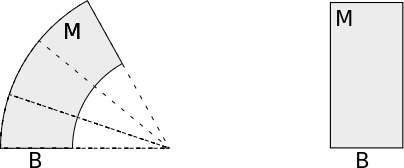
\includegraphics[width=.9\linewidth]{../img/RiemannFibration.png}
\caption{The trivialising map is only a diffeomorphism and not an isometry \label{trivalising-map}}
\end{figure}





\begin{theorem}[Hermann]
\label{thm:Hermann}
If the fibration \(\pi: M \longrightarrow B\) is
of totally geodesic fibres then the diffeomorphisms \(\hat\gamma(0) \longrightarrow
\hat\gamma(1)\) are in fact isometries between fibres and \(M\) is then locally a
Riemannian product of \(B\) and the fibre, now equipped with its unique
metric induced by \(M\).
\end{theorem}

\begin{proof}
We need to prove that the metric on fibres \(\hat g_{(b,f)}\) does not depend on the point
\(f\) of the fibre, i.e. for every basic vector field \(X\), one has \(\mathcal{L}_X\hat g=0\), where by \(\hat g\), we mean the (0,2) symmetric tensor \((Y_1, Y_2)\mapsto \langle
\mathcal{V}Y_1, \mathcal{V}Y_2 \rangle\). Let \(U,V\) be vertical vector fields of \(M\) then
\begin{equation*}
\label{eq:calcul-Hermann}
\begin{split}
X(\hat g(U,V)) &= (\mathcal{L}_X \hat g)(U,V) + \hat g([X,U],V) + \hat g(U, [X,V])\\
       	       &=  \langle \nabla_X U, V \rangle - \langle \nabla_U X, V \rangle + \langle U, \nabla_X V \rangle - \langle U, \nabla_V X \rangle + (\mathcal{L}_X\hat g)(U,V)
\end{split}   
\end{equation*}
Hence \((\mathcal{L}_X \hat g)(U,V) = \langle \nabla_U X, V\rangle + \langle U, \nabla_V
X \rangle = -2 \langle \sff(U,V), X \rangle = 0\). Since the map \(\hat\gamma(0) \mapsto \hat\gamma(1)\) is in the one-parameter group of differomorphism
associate to a basic vector field \(X\), it preserves \(\hat g\).
\end{proof}

\subsubsection{Tension fields and harmonic fibrations.}
\label{sec:orgae5582c}
We will now calculate the tension field of a fibration map \(\pi: M \longrightarrow B\).

\begin{proposition}[]
\label{prop:tension-fibration}
Let \(\pi: M^n \longrightarrow B^{n'}\) be a complete Riemannian fibration then
\begin{enumerate}
\item \(e(\pi) = n/2\).
\item Let \(M_b\) be a fibre of \(\pi\) and \(\iota_{M_b}: M_b \hookrightarrow M\) be
the inclusion. Then \(\tau(\pi) = -\pi_*\tau(\iota_{M_b})\) on \(M_b\).
\end{enumerate}
In particular, \(\pi\) is harmonic if and only if its fibres are minimal submanifolds of
\(M\), i.e. the inclusions \(\iota_{M_b}\) are harmonic.
\end{proposition}
\begin{proof}
\begin{enumerate}
\item is obvious. For 2), note that
\end{enumerate}
\[
\tau(\iota_{M_b}) = -\sum_{\sigma = 1}^{n'}{\rm div\ }(e_\sigma(P))e_\sigma(P)
\]
for any orthonormal frame \(e_\sigma(P)\) of normal vectors of \(M_{\pi(P)}\).
Take \(e_\sigma\) to be \(e_\sigma = {\rm grad\ } \pi^\sigma\) where \(\pi^\sigma\)
is the \(\sigma\)-th component of \(\pi\) in a normal coordinate of \(V\) around \(\pi(P)\). Note that \(e_\sigma\) are actually the horizontal lift of the basis vectors \(\tilde e_\sigma\) of the frame at \(\pi( P)\), and therefore are normal vectors of \(M_P\). 

Meanwhile, one has \(\tau(\pi) = -\Delta \pi^\sigma \tilde e_{\sigma}\) at \(\pi(P)\)
since the Christoffel symbols vanish at \(P\). Comparing the two vector fields, one has
\(\tau(\pi) = -\pi_*\tau(\iota_{M_b})\) at \(P\).
\end{proof}

\begin{exampl}
A complete Riemannian fibration \(\pi: M \longrightarrow B\) with totally geodesic fibres are harmonic.
\end{exampl}

\fi

\subsection{Composition of maps}
\label{sec:org929ef26}

The following results come from direct computation of the second fundamental form and
tension field of composition of maps between Riemannian manifolds. Again, we use indices
\(i,j,k,\dots\) for \(M\), \(\alpha,\beta,\gamma,\dots\) for \(M'\) and \(a,b,c,\dots\) for \(M''\).

\begin{proposition}
\label{prop:composition-general}
Let \(f: M \longrightarrow M'\) and \(f': M' \longrightarrow M''\) be smooth maps of
Riemannian manifolds, then
\begin{equation}
\label{eq:sff-composition}
\beta(f'\circ f)^a_{ij} = \beta(f)_{ij}^\gamma f'^a_\gamma + \beta(f')_{\alpha\beta}^a f^\alpha_i f^\beta_j
\end{equation}
and
\begin{equation}
\label{eq:tension-field-composition}
\tau(f'\circ f)^a = \tau(f)^\gamma f'^a_\gamma + g^{ij}\beta(f')^a_{\alpha\beta} f^\alpha_i f^\beta_j 
\end{equation}
Therefore,
\begin{center}
\begin{tabular}{lll}
If \(f'\) is & and \(f\)  is & then \(f'\circ f\) is\\
\hline
totally geodesic & totally geodesic & totally geodesic\\
totally geodesic & harmonic & harmonic\\
\end{tabular}
\end{center}
and the inverse of a totally geodesic map is totally geodesic.
\end{proposition}


\begin{remark}
It is not true in general that the composition of harmonic maps are harmonic. For example,
if one composes the harmonic maps \(\mathbb{R} \longrightarrow
\mathbb{R}^2: x \mapsto (x,2x)\) and \(\mathbb{R}^2 \longrightarrow
\mathbb{R}: (x,y)\mapsto x^2 - y^2\), the result is \(\mathbb{R}\longrightarrow \mathbb{R}: x \mapsto -3x^2\),
which is not harmonic.
\end{remark}

\begin{proposition}[composition with immersion]
\label{prop:compo-immersion}
If \(f': M' \longrightarrow M''\) is a Riemannian immersion and \(f: M \longrightarrow
M'\) then 
\begin{enumerate}
\item Energy functionals: \(E(f) = E(f'\circ f)\).
\item Tension fields: \(\tau(f)\) is the projection of \(\tau(f'\circ f)\) to \(M'\).
\end{enumerate}
\end{proposition}
\begin{proof}
\begin{enumerate}
\item One has \(e(f) = \frac{1}{2}\langle g, f^* g' \rangle  = \frac{1}{2}\langle g,
   (f'\circ f)^* g'' \rangle = e(f'\circ f)\).
\item One has \(\tau(f'\circ f)^a  = \tau(f)^a +
   g^{ij}\beta(f')^a_{\alpha\beta} f^\alpha_i f^\beta_j\) by
\eqref{eq:tension-field-composition}. The conclusion follows since the second term is normal to \(M'\), .
\end{enumerate}
\end{proof}

The following immediate corollary of Proposition \ref{prop:compo-immersion} is a generalization of the fact that a curve is geodesic if and only if it
is perpendicular to its tension field.

\begin{corollary}
If \(f': M' \longrightarrow M''\) is a Riemannian immersion, then a map \(f: M \longrightarrow M'\) is harmonic if and only if \(\tau(f'\circ f) \perp M'\).
\end{corollary}


\iffalse


\begin{proposition}[composition with submersion]
\label{prop:compo-submersion}
Let \(f': M' \longrightarrow M''\) be a Riemannian fibration with totally geodesic
fibres and \(f: M \longrightarrow M'\) then 
\[
\tau(f'\circ f) = f'_*(\tau(f))  
\]
\end{proposition}

\begin{proof}
One can suppose that \(M'\) is a Riemannian product of \(M''\) and its fibre, and
\(f'\) is the projection to \(M''\), since this is true locally and the proposition is
local. Then the conclusion is that the tension field of the projection is the projection
of the tension field, or equivalently the tension field of \(f= f_1\times f_2: M \longrightarrow
M''\times F\) is \(\tau(f) = (\tau f_1,\tau f_2)\). This follows from the explicit
formula of \(\tau(f)\), noting that the Christoffel symbols \(\Gamma^\alpha_{\beta\gamma}\) vanish except when the indice \(\alpha,\beta,\gamma\)
belong to the same tangent space (\(TM''\) or \(TF\)).
\end{proof}

\begin{exampl}
\begin{enumerate}
\item A map \(f: M \longrightarrow M'\times M''\) is harmonic if \(f=(f^1, f^2)\) with \(f^1, f^2\) harmonic.
\item Take \(M''=M\) in Proposition \ref{prop:compo-submersion} and \(f=s: M \longrightarrow M'\) a
section of the fibration \(f'\), one sees that the tension field \(\tau(s)\) is
always vertical.
\end{enumerate}
\end{exampl}

The following corollary is immediate.
\begin{corollary}
\label{cor:compo-with-submersion}
Let \(f': M' \longrightarrow M''\) be a proper Riemannian embedding and \(N\) is a
normal turbular neighborhood of \(M'\) which can be seen as a smooth fiber bundle over
\(M'\). Denote by \(\pi: N \longrightarrow M'\) the projection. Then for all map \(f:
M \longrightarrow N\), \(\pi\circ f\) is harmonic if and only if \(\tau(f)\) is vertical. 
\end{corollary}

\fi



\section{Nonlinear heat flow: Global equation and existence of harmonic maps.}
\label{sec:orgec9b5c0}
\subsection{Statement of the main results.}
\label{sec:org6fcf717}

We want to prove in the next part the existence of harmonic map between manifolds \(M\)
and \(M'\) by deforming any map \(f: M
\longrightarrow M'\) using the \(\tau\)-flow, meaning solving the PDE:
\begin{equation}
\label{eq:loc-heat-flow}
\begin{cases}
\frac{d f_t}{d t} = \tau (f_t),  & t\in [\alpha,\omega] \\
f_\alpha = f, & 
\end{cases}
\end{equation}
The equation makes sense because both \(\frac{d f_t}{d t}\) and \(\tau (f_t)\) are
vector fields along \(f_t\). Since this is the gradient-descent equation for \(E\),
the energy of \(f_t\) decreases and we hope, under conditions, to obtain
convergence of \(\{f_t\}\) to a critical point \(f_\infty\) of \(E\), this will prove
that any homotopy class of \(C^\infty(M,M')\) has at least a harmonic map.

It is proved by Eells and Sampson \cite{eells_harmonic_1964} that
\begin{theorem}[Eells-Sampson]
\label{thm:eells-sampson}
Let \(M\) and \(M'\) be compact Riemannian manifolds with \({\rm Riem } (M') \leq 0\) then there exists a harmonic map \(f: M \longrightarrow M'\) in each homotopy class.
\end{theorem}

Several boundary conditions, of Dirichlet, Neumann or mixed type, are also taken into account by Hamilton
\cite{hamilton_harmonic_1975}, as an example, we will state the Dirichlet problem:

\begin{theorem}[Hamilton]
\label{thm:hamilton-bndry-Dirichlet}
Let \(M\) and \(M'\) be compact Riemannian manifolds possibly with boundary. Suppose
that \(M'\) has \({\rm Riem } (M')\leq 0\) and \(\partial M'\) is convex, then any
relative homotopy class of \(C^\infty(M,M')\) has a harmonic element. 
\end{theorem}

About the terminology, \textbf{relative homotopy class} means that we only deform \(f\) among
maps with the same value on \(\partial M\). The \textbf{convexity of \(\partial M'\)} means
that the geodesic at any point in \(\partial M'\) with initial tangent vector parallel
to the boundary does not enter the interior of \(M'\) in short time. This condition can be expressed
using  the Christoffel symbols of \(M'\) at the point in question: If \(M'\) is
coordinated by \(y^1,\dots,y^n\) with and \(M' =\{y^n\geq 0\}\), then the convexity is
translated as \(\Gamma'^n_{\alpha\beta} \geq 0\) as a symmetric form (\(1\leq\alpha,\beta \leq n-1\)). This can be seen by the geometric intepretation of the second fundamental form of the
embedding \(s: \partial M' \hookrightarrow M'\), which is \(\sff(s) = -\Gamma'^n_{\alpha\beta}\).

It is easy to see that the convexity of \(\partial M'\) is a necessary condition, as
harmonic maps from \(\mathbb{R}\) are geodesics: Suppose the condition does not hold at
\(x\in \partial M'\), meaning that upto time \(t\) the geodesic flow of \(M'\) initially tangent to
\(\partial M'\) remains in the interior. The geodesic of \(\partial M'\) of length
less than \(t\) with the same initial tangent therefore cannot be deformed into a
geodesic of \(M'\) in relative homotopy class. 

\subsection{Strategy of the proof.}
\label{sec:orgab9af17}
In order to have a global frame, we will embed \(M'\) into an Euclidean space \(V\),
but we will not use the Euclidean metric of \(V\). In fact, let \(T\) be a tubular
neighborhood of \(M'\) in \(V\) then if \(T\) is trivial, i.e. if it is diffeomorphic to \(M'\times D\)
where \(D\) is a sufficiently small of dimension being the codimension of \(M'\) in \(V\), and we will equip \(T\) with the product metric of \(M'\times D\). 

If \(T\) is not trivial, using a partition of unity of \(M'\), one can construct a metric on \(T\)
as linear combination of the product metrics on trivialised pieces so that
the involution \(\iota: T \longrightarrow T\) locally given by \((y,d)\mapsto (y,-d)\)
for \(y\in M', d\in D\) is an isometry. As a consequence, \(M'\) is totally geodesic
in \(T\).


Since \(M' \equiv M'\times \{0\}\) is totally geodesic in \(T\), one has for every smooth
function \(f: M \longrightarrow M'\):
\[
 \tau_T(f) = \tau_{M'} (f)
\]

The crucial property we expect for a global equation of \eqref{eq:loc-heat-flow}, is the following: if
the solution initially is in \(M'\subset V\) then it remains in \(M'\) for all
relevant time \(t>\alpha\). Eells-Sampson \cite{eells_harmonic_1964} did this by using at
the same time 2 different metrics on \(T\), namely the product metric as tubular
neighborhood and the Euclidean metric. I choose to present here the formulation of
Hamilton, which is conceptually simpler with the only drawback being that we need to
establish the uniqueness of solution of \eqref{eq:loc-heat-flow} first.

After having the global equation, we will prove the short time existence of solution by
linearising the equation and using Inverse function theorem. The global formulation and the
proof of short-time existence is independent of the negative curvature hypothesis, which
will only be used later to establish energy estimates and assure the convergence of
long-time solution and the vanishing of its tension field.


\subsection{Global equation and Uniqueness of nonlinear heat equation.}
\label{sec:orgb597761}
\begin{theorem}[Global equation]
\label{thm:global-eq}
If the smooth function \(F_t:\ M\times [\alpha,\beta] \longrightarrow V\) satisfies
\begin{equation}
\label{eq:global-heat}
\frac{d F_t}{dt} = \tau_T(F_t)
\end{equation}
and \(F_t(M\times \{\alpha\}) \subset M'\) then \(F_t(M\times[\alpha,\omega])\subset M'\)
\end{theorem}
\begin{proof}
Let \(\iota\) be the isometry of \(T\) locally given by \((y,d)\mapsto (y,-d)\) for \((y,d)\in M'\times D \equiv T\) 
and pose \(G_t= \iota F_t\) then \(G_t\) and \(F_t\) coincide initially since \(M'\) is
fixed by \(\iota\). Moreover
\[
\frac{d G_t}{d t} = d\iota . \frac{d F_t}{d t} = d\iota (\tau_T(F_t)) = \tau_T(\iota F_t)=\tau_T(G_t)
\]
We conclude that \(F_t = G_t = \iota F_t\), hence \(F_t\) remains in \(M'\) for all
relevant \(t\), using the following uniqueness of nonlinear heat equation.
\end{proof}

\begin{theorem}[Uniqueness of solution of nonlinear hear equation]
\label{thm:unique-nonlinear-heat}
Let \(f_1,f_2: M\times [\alpha,\omega] \longrightarrow M'\) be \(C^2\)
functions satisfying the non-linear heat equation
\(\frac{d f_i}{d t} = \tau_{M'}(f_i)\), i.e.
\[
 \frac{d f_i}{d t} =-\Delta f^\gamma +g^{ij}\Gamma'^{\gamma}_{\alpha\beta} f^{\alpha}_{i}f^{\beta}_{j}
\]
where \(\Gamma'^\gamma_{\alpha\beta}\) are Christoffel symbols of \(M'\). Suppose that
\(f_1\) and \(f_2\) coincide on \(M\times \{\alpha\}\). Then \(f_1=f_2\) on \(M\times[\alpha,\omega]\).
\end{theorem}

\begin{proof}
It is sufficient to prove the theorem for \(\omega\) very close to \(\alpha\),
therefore by compactness of \(M\), we can suppose that there exists a finite atlas \(M
= \bigcup_i U_i\) with \(f_1 (U_i\times [\alpha,\omega])\) and \(f_2
(U_i,[\alpha,\omega])\) being in the same chart \(V_i\) of \(M'\). We consider the
distance function \(\sigma(a,b) = \frac{1}{2}d_{M'}(a,b)^2\) for \(a,b\in M'\) to
measure the difference between \(f_1\) and \(f_2\) by 
\[
 \rho(x,t) = \sigma(f_1(x,t), f_2(x,t))
\]
The strategy is to prove that there exists \(C>0\) such that \(\frac{d \rho}{d t} \leq
-\Delta \rho + C\rho\), then by \href{elliptic-parabolic.org}{Maximum principle}, one has \(\rho = 0\).

Fix a chart \(U_i\) of \(M\) and the corresponding \(V_i\) of \(M'\), one has by
straightforward calculation:
\begin{align}
 \frac{d\rho}{d t} &= -\Delta \rho -g^{ij}\left( \frac{\partial^2 \sigma}{\partial
 f_1^\beta \partial f_1^\gamma} - \frac{\partial \sigma}{\partial f_1^\alpha} {\Gamma'}
^{\alpha}_{\beta\gamma}(f_1) \right) {f_1}^\beta_i {f_1}^\gamma_j \nonumber \\
	        &- g^{ij}\left( \frac{\partial^2 \sigma}{\partial
 f_2^\beta \partial f_2^\gamma} - \frac{\partial \sigma}{\partial f_2^\alpha} {\Gamma'}
^{\alpha}_{\beta\gamma}(f_2) \right) {f_2}^\beta_i {f_2}^\gamma_j - 2g^{ij}\frac{\partial^2 \sigma}{\partial f_1^\beta \partial f_2^\gamma} {f_1}^\beta_i {f_2}^\gamma_j  \label{eq:drho-dt}
\end{align}
where \(g^{ij}\) is the metric on \(M\) and \({\Gamma'}^\alpha_{\beta\gamma}\) are
Christoffel symbols of \(M'\). 


Let \(c\) be a point in the chart \(V_i\) and choose the normal coordinates of \(M'\) at \(c\). Then for \(a,b\in M'\) near \(c\), one has, since \(\sigma(a,b) =
\sigma(b,a)\) and \(\sigma(a,b)=0\) if \(b^\gamma = k a^\gamma\) (the Euclidean
straight line from \(a\) to \(ka\) viewed on \(M'\) is a geodesic):
\[
 \sigma(a,b) = \frac{1}{2}d_{M'}(a,b)^2 = \frac{1}{2}d_E(a,b)^2 +
\lambda_{\beta\gamma,\delta}(a^\beta a^\gamma b^\delta + b^\beta b^\gamma a^\delta)
\]
where \(d_E\) is the Euclidean distance, with \(\lambda_{\beta\gamma,\delta} =
\lambda_{\gamma\beta,\delta}\) and \(\lambda_{\beta\gamma,\delta}
+\lambda_{\gamma\delta,\beta} + \lambda_{\beta\delta,\gamma}= 0\). We then have the
series development of \(\sigma\) at \((0,0)\):
\begin{equation}
\label{eq:dev-sig-unique}
\sigma(a,b) = \frac{1}{2}\delta_{\beta\gamma} (a^\beta - b^\beta)(a^\gamma - b^\gamma) +
\lambda_{\beta\gamma,\delta} (a^\beta a^\gamma b^\delta + b^\beta b^\gamma a^\delta) + O(|a|+|b|)^4
\end{equation}
and the development of its derivatives
\begin{align*}
  \frac{\partial^2 \sigma}{\partial a^\beta \partial b^\gamma}(a,b) &= -\delta_{\beta\gamma} + \lambda_{\beta\delta,\gamma}a^\delta + \lambda_{\gamma\delta,\beta}b^\delta + O(|a|+|b|)^2\\
  \frac{\partial^2 \sigma}{\partial a^\beta \partial a^\gamma}(a,b) &= \delta_{\beta\gamma} + \lambda_{\beta\gamma,\delta}b^\delta + O(|a|+|b|)^2\\
  \frac{\partial^2 \sigma}{\partial b^\beta \partial b^\gamma}(a,b) &= \delta_{\beta\gamma} + \lambda_{\beta\gamma,\delta}a^\delta + O(|a|+|b|)^2\\
   \frac{\partial\sigma}{\partial a^\alpha}(a,b) &= O(|a|+|b|),\quad {\Gamma'}^\alpha_{\beta\gamma}(a) = O(|a|)
\end{align*}
So choose \(c\) to be the midpoint of \(f_1(x,t)\) and \(f_2(x,t)\) and \((f_1(x,t),
f_2(x,t)) = (w,-w)\) in the chart, one has:
\begin{align}
 \frac{d\rho}{d t} &= -\Delta\rho - \left( \delta_{\beta\gamma} -\lambda_{\beta\gamma,\delta}w^\delta + O(|w|^2)  \right) {f_1}^\beta_i {f_1}^\gamma_j g^{ij}   - \left( \delta_{\beta\gamma} + \lambda_{\beta\gamma,\delta} w^\delta + O(|w|^2)\right) {f_2}^\beta_i {f_2}^\gamma_j g^{ij}  \label{eq:sym-red-beta-before}\\
		   & - 2\left( -\delta_{\beta\gamma} + \lambda_{\beta\delta,\gamma}w^\delta - \lambda_{\gamma\delta,\beta} w^\delta + O(|w|^2)  \right) {f_1}^\beta_i {f_2}^\gamma_j g^{ij} \label{eq:sym-red-beta}\\
		   & = -\Delta \rho - |df_1 -df_2|^2 - w^\delta \lambda_{\beta\gamma,\delta}g^{ij}\left(  {f_2}^\beta_i {f_2}^\gamma_j - {f_1}^\beta_i {f_1}^\gamma_j  \right) \label{eq:first-order-w}
\end{align}
where we made a reduction of the term \eqref{eq:sym-red-beta}, using the symmetric role of \(\beta\) and
\(\gamma\) to cancel the first order term \(w^\delta\). This symmetry is not apparent
in the term \eqref{eq:sym-red-beta} itself, but can be seen through their symmetry in the
2 terms of \eqref{eq:sym-red-beta-before} and their symmetry in the sum of all three,
i.e. in the RHS of \eqref{eq:drho-dt}. The last term of \eqref{eq:first-order-w} can be bounded as follows:
\begin{align*}
    \left | w^\delta \lambda_{\beta\gamma,\delta}\left({f_2}^\beta_i {f_2}^\gamma_j -
{f_1}^\beta_i {f_1}^\gamma_j\right) g^{ij} \right| &=   \left | w^\delta \lambda_{\beta\gamma,\delta}\left({f_2}^\beta_i ({f_2}^\gamma_j - {f_1}^\gamma_j) + {f_1}^\gamma_j({f_2}^\beta_i -
{f_1}^\beta_i) \right) g^{ij} \right| \\
	       &\leq 2 |w^\delta \lambda_{\beta\gamma,\delta}| |df_2 -df_1| (|df_1| + |df_2|)\\
	       &\leq |df_1 - df_2|^2 + O(|w|^2)
\end{align*}
where for the last inequality, we use \(2uv \leq u^2 + v^2\) and the fact that \(|df_1|\) and \(|df_2|\) are bounded on \(M\). The estimate \eqref{eq:first-order-w} can be
continued:
\[
 \frac{d \rho}{d t}\leq -\Delta\rho + C(x,t) |w|^2 \leq -\Delta \rho + C \rho
\]
where \(C >0\) is a constant chosen to dominate all \(C(x,t)\) for \(x\in M\) in all
charts and \(t\in [\alpha,\omega]\).
\end{proof}

\begin{remark}
\label{rem:hamilton-alg-rig}
The original proof of \cite{hamilton_harmonic_1975}
made the reduction of the first order of \(w\) in \eqref{eq:sym-red-beta} using
the following development of \(\sigma\):
\[
 \sigma = \frac{1}{2}\delta_{\beta\gamma} (a^\beta - b^\beta)(a^\gamma - b^\gamma) +
\lambda_{\beta\gamma,\delta} (a^\beta - b^\beta)(a^\gamma -b^\gamma)(a^\delta + b^\delta) + O(|a|+|b|)^4
\]
which was justified by \(\sigma(a,b) = \sigma(b,a)\) and \(\sigma(a,a)=0\). It can be proved this is equivalent to \eqref{eq:dev-sig-unique} and the symmetries \(\lambda_{\beta\gamma,\delta} =
\lambda_{\gamma\beta,\delta},\ \lambda_{\beta\gamma,\delta}
+\lambda_{\gamma\delta,\beta} + \lambda_{\beta\delta,\gamma}= 0\).

As a side note, if \(a,b,c\) are on \(\mathbb{S}^2\) with \(d(a,c) = d(b,c) = x \ll 1\)
and the lines from \(a\) and \(b\) to \(c\) are orthogonal at \(c\), then the
geodesic distance \(d(a,b) = \arccos(\cos^2(x)) = x\sqrt{2} - \frac{1}{6\sqrt{2}}x^3 +
O(x^4)\). So \(\sigma(a,b) = \frac{1}{2}d(a,b)^2\) has no third-order term.
\end{remark}

\section{A few energy estimates.}
\label{sec:org1f4fa53}
\subsection{Estimate of density energies}
\label{sec:org3c01090}
We finish this part with a few straightforward computation concerning the \textbf{potential
energy} \(e(f_t) = \frac{1}{2}|\nabla f_t|^2\) and the \textbf{kinetic energy} \(k(f_t) =
\frac{1}{2}|\frac{d f_t}{d t}|^2\) of a nonlinear heat flow \(f_t\)
satisfying \eqref{eq:loc-heat-flow}.

\begin{theorem}[Density of Potential energy]
\label{thm:den-pot}
If \(f_t\) satisfies \eqref{eq:loc-heat-flow} then 
\[
 \frac{d e(f_t)}{dt}= -\Delta e(f_t) - |\beta(f_t)|^2 - \left\langle \Ric(M) \nabla_v
f_t,\nabla_v f_t \rangle + \langle \Riem(M') (\nabla_v f_t,\nabla_w f_t)\nabla_v
f_t,\nabla_w f_t \right\rangle
\]
where \(e(f_t)\) is the potential energy density and \(\beta(f_t)\) is the fundamental
form and in the curvature terms, the vectors \(v\) and \(w\) are contracted.

In particular, if  \(\Riem(M') \leq 0\) and \(\Ric(M)\geq -C\) then
\begin{equation}
\label{eq:den-pot-est}
\frac{d e}{dt} \leq -\Delta e + Ce - |\beta(f_t)|^2
\end{equation}
\end{theorem}
\begin{proof}
Apply Lemma \ref{lem:calculs-general} to \(s = d f_t\) and the Riemannian-connected
bundle \(F^* TM'\) over \(M\times [\alpha,\omega]\) where \(F(\cdot,t) = f_t\), the curvature terms cancel
out and it remains to see that
\(\frac{d e(f_t)}{dt}= - \langle df_t, \Delta df_t \rangle\), meaning that \(\tilde \nabla_{\partial t} df_t = -\Delta df_t\). This can be easily
justified:
\[
\tilde \nabla_{\partial t} df_t = \tilde \nabla_{\partial t} \tilde\nabla^M F=  \tilde\nabla^M
\tilde\nabla_{\partial t} F= \tilde\nabla^M\ \tau (f_t) = -D\delta (df_t) = -\Delta df_t
\]
where the last "=" is due to \(D df_t = 0\). Note that \(D\) and \(\delta\)
are the exterior derivative and its adjoint of the bundle \((f_t)^*TM'\) on \(M\),
where \(t\) can be fixed after the third "=" sign.
\end{proof}

\begin{theorem}[Density of Kinetic energy]
\label{thm:den-kin}
If \(f_t\) satisfies \eqref{eq:loc-heat-flow} then 
\[
 \frac{d k(f_t)}{dt}= -\Delta k(f_t) - \left|\nabla \frac{\partial f_t}{\partial t}\right|^2 +
\left\langle \Riem(M') (\nabla_v f_t,\frac{\partial f_t}{\partial t})\nabla_v
f_t,\frac{\partial f_t}{\partial t} \right\rangle
\]
where \(k(f_t)\) is the kinetic energy density and in the curvature terms, the vectors \(v\) is contracted,

In particular, if  \(\Riem(M') \leq 0\) then
\begin{equation}
\label{eq:den-kin-est}
\frac{d k}{dt} \leq -\Delta k  - \left|\nabla \frac{\partial f_t}{\partial t}\right|^2
\end{equation}
\end{theorem}

\begin{proof}
Let \(F:\ I\times M \longrightarrow M'\) be the total function with \(F(t,\cdot)
= f_t\) for \(t\in I =[\alpha,\omega]\) and \(E = F^* TM'\) is a Riemannian-connected bundle on \(I\times M\) with curvature form \(\Theta\), then
\begin{equation}
\label{eq:den-kin-1}
\tilde \nabla_{\partial t} \tilde\nabla_v (dF.v) = \tilde\nabla_v \tilde\nabla_{\partial t} (dF.v) + \Theta(\partial t, v) dF.v
\end{equation}
where \(dF\) is the exterior derivative of \(f_t\) on \(M\). Note that \(\tilde \nabla_v \tilde \nabla_{\partial t} (dF.v) = \tilde \nabla_v (\tilde
\nabla_{\partial t} dF).v = \tilde \nabla_v (\tilde\nabla^M \frac{\partial f_t}{\partial
t}).v\) since \(\tilde\nabla^M \frac{\partial f_t}{\partial t}= \tilde\nabla_{\partial
t}^{I\times M} dF = \tilde\nabla^{I}_{\partial_t}dF\) because
\(\tilde \nabla\) is torsionless on \(M'\). Plugging this in \eqref{eq:den-kin-1} and taking contraction
in \(v\), one has
\begin{equation}
\label{eq:den-kin-2}
 \tilde \nabla_{\partial t}\ \tau(f_t) = -\tilde \Delta \frac{\partial f_t}{\partial t} +
\tr \left( v\mapsto \Theta (\partial t,v) dF.v\right)
\end{equation}
But \(\Theta^\beta_\alpha = R'^\beta_{\alpha\nu\mu} F^\mu_i F^\nu_j dx^i\otimes dx^j\)
where \(R'\) denotes the Riemannian curvature of \(M'\) and the indices \(i,j\) can
be \(0\), with \(x^0 \equiv t\). Hence 
\[
 \Theta (\partial t, v) dF.v = R'^\beta_{\alpha \nu \mu} \frac{\partial f^\mu_t}{\partial
t}\frac{\partial f_t^\nu}{\partial v} \frac{\partial f_t^\alpha}{\partial v} \tilde
e_\beta = \Riem(M')\left(\nabla_v f_t, \frac{\partial f_t}{\partial t}\right)\nabla_v f_t
\]
Plugging in \eqref{eq:den-kin-2} and taking inner product with \(\frac{\partial
f_t}{\partial t}\), one has
\begin{align*}
 \frac{\partial k(f_t)}{\partial t} &= \left\langle \tilde \nabla_{\partial t}\ \tau(f_t),
\frac{\partial f_t}{\partial t} \right \rangle = - \left\langle \tilde \Delta \frac{\partial
f_t}{\partial t}, \frac{\partial f_t}{\partial t} \right\rangle + \left \langle \Riem(M')
(\nabla_v f_t, \frac{\partial f_t}{\partial t}) \nabla_v f_t, \frac{\partial f_t}{\partial
t} \right \rangle  \\
   &= - \Delta \left(\frac{1}{2} \left|\frac{\partial f_t}{\partial t}\right|^2\right) - \left| \tilde \nabla \frac{\partial f_t}{\partial t}\right|^2 + \left \langle \Riem(M')
(\nabla_v f_t, \frac{\partial f_t}{\partial t}) \nabla_v f_t, \frac{\partial f_t}{\partial
t} \right \rangle
\end{align*}
\end{proof}

\subsection{Estimate of total energies}
\label{sec:orge212cfb}

We will now work with the total energies, in particular the \textbf{total potential energy} \(E(f_t) := \int_M e(f_t)\) and \textbf{total kinetic energy} \(K(f_t) := \int_M k(f_t)\). Since
tension field is the gradient of \(E\), one has:

\begin{theorem}
\label{thm:energy-cons}
If \(f_t: M \longrightarrow  M'\) satisfies \eqref{eq:loc-heat-flow} then
\[
 \frac{d E(f_t)}{dt} = -\int_M \left\langle \tau(f_t), \frac{\partial f_t}{\partial t}
\right \rangle = -\int_M |\tau(f_t)|^2 = -2K(f_t) \leq 0
\]
and
\[
\frac{d^2 E(f_t)}{dt} = -2\int_M \left \langle \nabla_{\partial t}\frac{\partial
f_t}{\partial t},\tau(f_t)\right \rangle
\]
\end{theorem}

Intergrating Theorem \ref{thm:den-kin} on \(M\) then using Theorem \ref{thm:energy-cons}, one obtains:

\begin{theorem}
\label{thm:int-den-kin}
If \(f_t\) satisfies \eqref{eq:loc-heat-flow} and \(\Riem(M')\leq 0\) then \(\frac{d
}{dt}K(f_t) \leq 0\) and one has
\begin{enumerate}
\item The total potential energy \(E(f_t)\) is \(\geq 0\), decreasing and convex.
\item The total kinetic energy \(K(f_t)\) is \(\geq 0\), decreasing and if \(\omega =
   +\infty\) then \(\lim_{t\to\infty} K(f_t) = 0\).
\end{enumerate}
In particular, \(\int_{M\times \{\tau\}} |\nabla f|^2\) and \(\int_{M\times\{\tau\}} \left|
\frac{\partial f_t}{\partial t} \right|^2\) are bounded above by a constant \(C>0\)
independent of the time \(\tau \in[\alpha,\omega]\).
\end{theorem}
Note that we ruled out the case \(K(f_t)\) decreases to a strictly positive limit
because \(E(f_t)\) is bounded below and \(\frac{d }{d t} E(f_t) = -2K(f_t)\).


Integrating Theorem \ref{thm:den-pot} on \(M\) then using Theorem \ref{thm:int-den-kin}, one has:

\begin{theorem}
\label{thm:int-den-pot}
If \(f_t\) satisfies \eqref{eq:loc-heat-flow} and \(\Riem(M')\leq 0\) and \(\Ric(M)\)
is bounded below then 
\[
\int_M |\beta(f_t)|^2 \leq C
\]
for all time \(t\) where the constant \(C\) only depends on the curvature of \(M, M'\) and the initial total potential and kinetic energy, in particular, \(C\) does not depend on \(t\).
\end{theorem}

This means that \(\|f_t\|_{W^{2,2}(M)}\) is bounded by a constant \(C\) only depending
on the curvatures and initial total energies.


\begin{corollary}[Boundedness in \( W^{2,2}(M) \)]
\label{cor:bound-2-2}
If \(F_t\) satisfies \eqref{eq:global-heat} and \(\Riem(M')\leq 0\) and \(\Ric(M)\)
is bounded below then
\[
\|F_t\|^2_{W^{2,2}(M)} := \int_M | \beta(F_t)|^2 + |\nabla F_t| +|F|^2 \leq C
\]
for all time \(t\) where the constant \(C\) only depends on the curvature of \(M, M'\) and the initial total potential and kinetic energy, in particular, \(C\) does not depend on \(t\).
\end{corollary}

Note that the term \(|F|^2\) is trivially bounded since the image of \(F\) remains in
an Euclidean ball \(B\).



\part{Resolution of nonlinear heat equation on manifold}
\chapter{Short-time existence and regularity for nonlinear heat equation}
\iffalse
\begin{info}
The PDF version of this page can be downloaded by replacing \texttt{html} in the its address by
\texttt{pdf}. 
For example \texttt{/html/sheaf-cohomology.html} should become \texttt{/pdf/sheaf-cohomology.pdf}.
\end{info}
\fi

We will establish in this part a regularity estimate for the quadratic term of nonlinear
heat operator use it to setup a bootstrap scheme that eventually will prove that any
sufficiently regular solution of nonlinear heat equation that is initially \(C^\infty\)
will be always \(C^\infty\).

We will also prove short-time existence using well-known method of Inverse
function theorem for Banach spaces. Since the solution is smooth, we can apply Theorem
\ref{thm:global-eq} to conclude that the it remains in \(M'\subset \mathbb{R}^N\).

\section{Review of Sobolev spaces and Linear equations.}
\label{sec:org3af8194}

The following results are well-known and their statements are written here in the case of our interest (linear heat equation on
manifold). A more careful formulation with complete proofs can be found in the
appendices.

\subsection{Sobolev spaces.}
\label{sec:orge4cbcfa}

Let \(M\) be a Riemannian manifold, the \emph{Sobolev spaces} \(W^{k,p}(M)\) on \(M\) can be defined as the completion of \(C^\infty(M)\) with respect to the Sobolev norms
\[ 
\|\varphi\|_{W^{k,p}} = \sum_{|\alpha|\leq k} \| D^\alpha \varphi \|_{L^p}. 
\]
We will suppose that \(M\) is a compact manifold, then set-theoretically \(W^{k,p}\) does not depend
on the metric of \(M\) and their norm remains in the same equivalent class as the metric
varies. The Sobolev spaces form a family of reflexive Banach spaces that is stable under holomorphic
interpolation:

\begin{theorem}[Interpolation of Sobolev spaces]
\label{thm:interp-sobolev-d}
Let \(p,q\in (1,+\infty)\) and \(k,l\in \mathbb{R}\) and \(M\) be a compact
Riemannian manifold. Then the holomorphic interpolations of 
\[
 A_0:= W^{k,p}(M)\quad \text{and}\quad A_1:=W^{l,q}(M)
\]
are \(A_\theta=W^{s,r}(M)\) where
\[
 \theta l + (1-\theta)k = s,\qquad \theta \frac{1}{q} + (1-\theta) \frac{1}{p} = \frac{1}{r}.
\]
In particular, one has the Interpolation inequality
\[
 \|f\|_{W^{s,r}}\leq 2 \|f \|^\theta_{W^{l,q}} \| f\|^{1-\theta}_{W^{k,p}}.
\]
\end{theorem}

Sobolev embeddings and Kondrachov theorem remain correct on manifold. 

\begin{theorem}[Sobolev embedding]
\label{thm:Sobolev-Rn-d}
Given \(k,l\in \mathbb{Z},\ k>l \geq 0\) and \(p,q\in \mathbb{R},\ p>q\geq 1\). Then
\begin{enumerate}
\item If \(\frac{1}{p}= \frac{1}{q} - \frac{k-l}{n}\) then 
\[
    W^{k,q}(M) \hookrightarrow W^{l,p}(M),
   \]
\item If \(\frac{k-r}{n}> \frac{1}{q}\) then
\[
   W^{k,q}(M) \hookrightarrow C^r(M)
   \]
If \(\frac{k-r-\alpha}{n}\leq \frac{1}{q}\) then 
\[ 
   W^{k,q}(M) \hookrightarrow C^{r,\alpha}(M) 
   \]
\end{enumerate}
where \(C^r(M)\) denotes the space of \(C^r\) functions equipped with the norm \(\| u \|_{C^r} = \max_{l\leq
r}\sup|\nabla^l u|\), and \(C^{r,\alpha}\) is the subspace of \(C^r\) of functions
whose \(r^{\rm th}\)-derivative is \(\alpha\)-Holder, equipped with the norm \(\|
u\|_{C^{r,\alpha}} = \| u \|_{C^r} + \sup_{P\ne Q}\{ \frac{u(P) - u(Q)}{d(P,Q)^\alpha} \}\).
\end{theorem}

\begin{theorem}[Kondrachov]
\label{thm:Kondrachov-Rn-d}
Let \(k\in \mathbb{Z}_{\geq 0}\) and \(p,q\in \mathbb{R}_{>0}\) be such that
\(1\geq \frac{1}{p} > \frac{1}{q} - \frac{k}{n} > 0\) then
\begin{enumerate}
\item The embedding \(W^{k,q}(M) \hookrightarrow  L^p(M)\) is compact,
\item The embedding \(W^{k,q}(M) \hookrightarrow  C^\alpha(M)\) is compact if
\(k-\alpha > \frac{n}{q}\) where \(0\leq \alpha < 1\),
\end{enumerate}
\end{theorem}

It is also natural, for regularity results of parabolic equation, to use weighted Sobolev
spaces because each derivative in time should be counted as twice as that in space. For
example, the space \(W^{2,p}(M\times[\alpha,\omega])\) is the completion of \(C^\infty(M)\) with respect to
the norm
\[
 \|\varphi\|_{W^{2,p}} := \|\varphi\|_{L^p} + \left\| \frac{d\varphi}{dt}\right\|_{L^p} + \sum_{i,j} \left\| \frac{\partial^2\varphi}{\partial x^i \partial
x^j} \right\|_{L^p} + \sum_i \left\| \frac{\partial\varphi}{\partial x^i} \right\|_{L^p}
\]
Similarly, one can define \(W^{2k,p}(M\times[\alpha,\omega])\) using \(L^p\)-norm of
derivatives \(\partial_t^\beta \partial_x^\gamma \varphi\) of \(\varphi\) with \(2\beta + \gamma
\leq 2k\).


We also want to be able to talk about \(W^{k,p}\) when \(k\) is not an integer and not necessarily positive. This
allows us to have a more flexible bootstrap scheme for nonlinear heat equation and to use
Interpolation Theorem \ref{thm:interp-sobolev-d} more efficiently. We claim that these
generalised Sobolev spaces (with weight and with non-integral regularity) can be defined on
manifold and satisfy all the above properties (reflexivity, Interpolation theorem, Sobolev
embedding and Kondrachov theorem) and refer to the appendices for all the details.

\subsection{Trace theorem.}
\label{sec:orgbc9f39d}

It is possible to avoid a discussion on Trace operator if we only want to make sense of the
initial condition of nonlinear heat equation: one can consider only solutions with
regularity greater than \(W^{2,p}(M\times[\alpha,\omega])\) with \(p \geq \dim M + 2\), which can be embedded in \(C(M)\). It is however necessary to investigate regularity of Trace operator to have a complete proof of the bootstrap. We will review
briefly some results.

The following two behaviors of trace are well-known:
\begin{enumerate}
\item If \(-1 + \frac{1}{p} < k < \frac{1}{p}\) then the natural map \(W^{k,p}(M\times[\alpha,\omega]/\alpha) \hookrightarrow W^{k,p}(M\times[\alpha,\omega])\) is an isomorphism, where \(W^{k,p}(M\times[\alpha,\omega]/\alpha)\) denotes the
completion under \(W^{k,p}\)-norm of the space of smooth functions vanishing on a
neighborhood of \(M\times \{\alpha\}\). There is therefore no meaningful notion of trace in this case.
\item If \(k > \frac{1}{p} + l,\ l\geq 0\), then the restriction map
\[
    B:\ C^\infty(M\times[\alpha,\omega]) \longrightarrow C^\infty(M):\ f(x,t) \longmapsto f(x,\alpha)
   \]
extends to a bounded operator \(B:\ W^{k,p}(M\times[\alpha,\omega]) \longrightarrow
   W^{l,p}(M)\), called \emph{Trace operator}.
\end{enumerate}

We will topologise the space \(\partial_\alpha W^{k,p}(M\times[\alpha,\omega])\) of
restrictions to time \(t=\alpha\) of functions in \(W^{k,p}(M\times[\alpha,\omega])\), in case Trace operator is well defined, as cokernel of
\(B\), that is, as a quotient
space of \(W^{k,p}(M\times[\alpha,\omega])\). This makes \(\partial_\alpha
W^{k,p}(M\times[\alpha,\omega])\) a Banach space with stronger norm than any \(W^{l,p}(M)\) for any \(l < k-\frac{1}{p}\).

\subsection{Linear equation on manifolds.}
\label{sec:orgb9f137c}

\subsubsection{Existence and Regularity.}
\label{sec:orgff9fdf8}

It can be easily verified that the linear heat operator \(AF:= \frac{d}{dt}F + \Delta F\)
is a parabolic operator and therefore is also an elliptic operator. All of the following results
holds for operator \(A\).

\begin{theorem}[Regularity for elliptic operator]
\label{thm:elliptic-d}
Let \(M\) be a compact manifold and \(AF:= \frac{d}{dt}F + \Delta F\) be an elliptic
operator of second order. Given \(\frac{1}{p} < l < k <\infty\) and \(F\in
W^{l,p}(M\times[\alpha,\omega])\) and suppose that 
\[
 AF\in W^{k-2,p}(M\times[\alpha,\omega]),\quad \restr{f}{\alpha}\in \partial_\alpha
W^{k,p}(M\times[\alpha,\omega]), \quad  \restr{f}{\omega}\in \partial_\alpha W^{k,p}(M\times[\alpha,\omega]).
\]
Then actually \(F\in W^{k,p}(M\times[\alpha,\omega])\).
\end{theorem}


\begin{theorem}[Causality of parabolic equation]
\label{thm:para-existence-d}
Let \(M\) be a compact manifold and \(AF:= \frac{d}{dt}F + \Delta F\) be an parabolic
operator. Then 
\[
 A:\ W^{k,p}(M\times[\alpha,\omega]/\alpha) \longrightarrow W^{k-2,p}(M\times[\alpha,\omega]/\alpha)
\]
is an isomorphism of Banach spaces.
\end{theorem}


\begin{theorem}[Gårding's Inequality and Regularity for parabolic operator]
\label{thm:para-eq-d }
Let \(M\) be a compact manifold, \(p\in (1,+\infty)\), \(k > l > -\infty\) and \(AF:= \frac{d}{dt}F + \Delta F\) be a parabolic operator. We write \(W^{k,p}([\beta,\gamma])\) shortly for \(W^{k,p}(M\times[\beta,\gamma])\). Suppose that
\[
 F\in W^{l,p}([\alpha,\omega]),\quad AF\in W^{k-2,p}([\alpha,\omega]).
\]
Then \(F\in W^{k,p}([\pi,\omega])\) for all \(\pi\in (\alpha,\omega)\). Also, there
exists a constant \(C>0\) such that 
\[
 \|F\|_{W^{k,p}([\pi,\omega])} \leq C \left( \|AF\|_{W^{k-2,p}([\alpha,\omega])} + \| F \|_{W^{l,p}([\alpha,\pi])}  \right).
\]
In particular for homogeneous equation, the solution is \(C^\infty\) and an arbitrarily weak estimate in the past gives an arbitrarily strong estimate in the future. 
\end{theorem}

\subsubsection{Maximum principle and Comparison theorems.}
\label{sec:orgf25e20e}
Other than regularity results which are generally true for parabolic operators, the linear
heat operator also enjoys the following versions of Maximum principle. See Appendices for
their proofs.

\begin{theorem}[Maximum principle]
\label{thm:max-princ-d}
Let \(M\) be a compact manifold and \(f: M\times[\alpha,\omega] \longrightarrow \mathbb{R}\) be a continuous function
with \(\restr{f}{\alpha}\leq 0\). Suppose that whenever \(f>0\), \(f\) is smooth and
\[
 \frac{\partial f}{\partial t} \leq -\Delta f + Cf.
\]
Then in fact \(f\leq 0\).
\end{theorem}

With the same proof as Theorem \ref{thm:max-princ-d}, one also has:

\begin{theorem}[\( L^\infty \)-Comparison theorem]
\label{thm:infty-comparison-d}
Let \(f: M\times[\alpha,\omega] \longrightarrow \mathbb{R}\) be a continuous function on
\(M\), smooth for all time \(t>0\) such that
\[
  \frac{d f}{dt} = -\Delta f + b f \text{ on } M\times (\alpha,\omega]
\]
where \(b\) is a smooth function on \(M\). Then there exists a constant \(B\) depending
only on \(b\) such that 
\[
 \|\restr{f}{\omega}\|_{L^\infty} \leq e^{B(\omega-\alpha)}
\|\restr{f}{\alpha}\|_{L^\infty}.
\]
\end{theorem}

Using backwards heat equation and Theorem \ref{thm:infty-comparison-d}, one can prove its
version for \(L^1\).

\begin{theorem}[\( L^1 \)-Comparison theorem]
\label{thm:1-comparison-d}
Let \(f: M\times[\alpha,\omega] \longrightarrow \mathbb{R}\) be a continuous function on
\(M\), smooth for all time \(t>0\) such that
\[
  \frac{d f}{dt} = -\Delta f + b f \text{ on } M\times (\alpha,\omega]
\]
where \(b\) is a smooth function on \(M\). Then there exists a constant \(B\) depending
only on \(b\) such that 
\[
 \|\restr{f}{\omega}\|_{L^1} \leq e^{B(\omega-\alpha)}
\|\restr{f}{\alpha}\|_{L^1}.
\]
\end{theorem}


\section{Regularity estimate of the quadratic term.}
\label{sec:org7baff5d}

\begin{theorem}[Regularity of the quadratic term]
\label{thm:reg-quad}
Let \(F:\ M\times [\alpha,\omega] \longrightarrow B\subset \mathbb{R}^N\) be in \(W^{s,q}(M\times[\alpha,\omega])\cap C(M\times [\alpha,\omega])\) and
\[ 
P F := g^{ij}\Gamma'^\alpha_{\beta\gamma}(F) F^\beta_i
F^\gamma_j.
\]
Suppose that
\begin{equation}
\label{eq:cond:thm:reg-poly-diff}
 r\geq 0,\quad p,q\in (1,\infty),\quad r+1 < s, \quad \frac{1}{p}> \frac{r+2}{s} \frac{1}{q}.
\end{equation}
Then one has \(PF\in W^{r,p}(X)\) and
\[
 \|P F \|_{W^{r,p}} \leq C\left(1 + \|F\|_{W^{s,q}}\right)^{q/p}.
\]
where \(C\) is a constant independent of \(F\).
\end{theorem}

\begin{proof}
We will suppose here that \(r,s\) are even integers so that the \(W^{r,p}\)
(respectively \(W^{s,q}\)) norm of \(PF\) (respectively \(F\)) can be written as sum of \(L^p\)
(respectively \(L^q\)) norms of its derivatives. Also, we will use chain rule freely to
differentiate the term \(\Gamma'^\alpha_{\beta\gamma}(F)\) using weak derivatives of \(F\). The general and rigorous proof, which involves fractional Sobolev space to treat non-integral
\(r, s\) and a detour to Besov spaces to justify chain rule, can be found in the appendices.

The derivatives of \(PF\) that appear in its \(W^{r,p}\) norm are of form
\[
 C(x,F)\ \prod_i \partial_t^{b_i} \partial_x^{c_i} F^{\beta_i} 
\]
where \(2\sum b_i + \sum c_i \leq r+2\) and \(\max \{2b_i+ c_i\}\leq r+1\) and \(C(x,F)\) is bounded on \(M\). Using Multiplication theorem for \(L^p\)-spaces, one has
\[
  \left\|C(x,F)\ \prod_i \partial_t^{b_i} \partial_x^{c_i} F^{\beta_i} \right\|_{L^p} \leq
\|C(x,F)\|_{L^\infty} \prod_i \left\|\partial_t^{b_i} \partial_x^{c_i}
F^{\beta_i}\right\|_{L^{p_i}}  \leq \|C(x,F)\|_{L^\infty} \prod_i \left\|F\right\|_{W^{2b_i+c_i,p_i}}
\]
as long as we choose \(p_i\in (1,\infty)\) such that \(\frac{1}{p} \geq \sum
\frac{1}{p_i}\). The
strategy is to choose \(\frac{1}{p_i}\) big enough to have \(W^{s,q}
\hookrightarrow W^{2b_i+c_i,p_i}\) in order to
bound \(\left\|F\right\|_{W^{2b_i+c_i,p_i}}\) by \(\left\|F\right\|_{W^{s,q}}\), then
use the upper bound of \(2b_i +c_i\) to justify that \(\frac{1}{p} > \frac{r+2}{s}
\frac{1}{q} \geq \sum \frac{1}{p_i}\), meaning that such choice of \(p_i\) are valid.

The straightforward way to have a sufficient condition of \(p_i\) such that \(W^{s,q}
\hookrightarrow W^{2b_i+c_i,p_i}\) is to use Sobolev embedding, but the result is sub-optimal
because Sobolev embedding does not take into account the \(L^\infty\)-bounded of \(F\) (its image lies in a compact of \(\mathbb{R}^N\)). A better way is to use
Interpolation inequality, by remarking that \(F\in W^{0,v}\) for all \(v\in (1,+\infty)\) and writing \(W^{2b_i+c_i, p_i}\) as an interpolation space of \(W^{s,q}\) and \(W^{0,v}\). It can be seen, by direct computation, that the sufficient condition for \(W^{s,q}
\hookrightarrow W^{2b_i+c_i,p_i}\) is \(2b_i+c_i < s\) and
\[
 0 < \frac{1}{p_i} - \frac{2b_i+c_i}{s}\frac{1}{q} < 1 - \frac{2b_i + c_i}{s}.
\]
Choose \(\frac{1}{p_i}\) just a bit bigger than \(\frac{2b_i+c_i}{s}\frac{1}{q}\), one
still has
\[
\sum \frac{1}{p_i} \simeq \sum  \frac{2b_i+c_i}{s}\frac{1}{q} \leq \frac{r+2}{s}\frac{1}{q} < \frac{1}{p}.
\]
The conclusion follows.  
\end{proof}



\section{Regularity for nonlinear heat equation.}
\label{sec:org703224a}
Let \(p>\dim M + 2\), using the regularity estimate for the quadratic term, we now can prove:

\begin{theorem}[Bootstrap for nonlinear heat equation]
\label{thm:reg-nonlin-heat}
Let \(F:\ M\times [\alpha,\omega] \longrightarrow B\) such that \(F\in W^{2,p}(M\times
[\alpha,\omega])\) and \(\frac{d F_t}{dt} = \tau(F_t)\), i.e.
\[
 \frac{d F^\alpha}{dt} = -\Delta F^\alpha + g^{ij}\Gamma'^\alpha_{\beta\gamma}(F)
F^\beta_i F^\gamma_j
\]
and \(\restr{F}{M\times\{\alpha\}}\) is smooth. Then \(F\) is smooth on \(M\times [\alpha,\omega]\).
\end{theorem}

\begin{remark}
Note that since \(p > \dim M + 2 = \dim (M\times [\alpha,\omega])+1\), if \(F\in
W^{2,p}(M\times[\alpha,\omega])\) then \(F\) and \(\frac{\partial F}{\partial
x^i}\) are in \(C(M\times[\alpha,\omega])\) by \href{sobolev-riemannian.org}{Sobolev embeddings}. It makes sense then to talk
about:
\begin{enumerate}
\item the restriction and boundary condition at time \(t=\alpha\) (in fact, by \href{interpolation-sobolev.org}{Trace theorem}, \(p>1\) is enough).
\item the pointwise condition \(F: M\times [\alpha,\omega] \longrightarrow
   B\subset V\).
\end{enumerate}
\end{remark}

\begin{proof}
We define the operators \(P F := g^{ij}\Gamma'^\alpha_{\beta\gamma}(F) F^\beta_i
F^\gamma_j\) and \(A F := \frac{dF }{dt} + \Delta F\). We will abusively denote \(W^{k,p}(M\times
[\beta,\gamma])\) by \(W^{k,p}([\beta,\gamma])\). Our bootstrap scheme consists of 3
steps:
\begin{enumerate}
\item Prove that \(F\in W^{2,\tilde p}([\pi,\omega])\) for every \(\pi > \alpha\) and \(\tilde p \in (1,\infty)\). By
compactness of \(M\), it is sufficient to prove this
for a sequence \(\tilde p \to +\infty\).
\item Prove that \(F\) is \(C^\infty\) for all time \(t >\alpha\).
\item Prove that \(F\) is \(C^\infty\) on \(M\times [\alpha,\omega]\).
\end{enumerate}

\emph{Step 1.} By Theorem \ref{thm:reg-quad}, \(AF = PF \in W^{r,q}([\alpha,\omega])\) whenever \(r<1\) and \(\frac{1}{q} > (\frac{r}{2}+1)\frac{1}{p}\). Apply Gårding inequality, for all
\(\pi >\alpha\), \(F\in W^{r+2,q}([\pi,\omega]) \subset W^{2,\tilde p}([\pi,\omega])\)
for \(\frac{1}{\tilde p} = \frac{1}{q} - \frac{r}{\dim M + 1}\). Choose \(\frac{1}{q}\) very close to \((\frac{r}{2}+1)\frac{1}{p}\), one sees that the condition on \(\tilde p\) is \(\frac{1}{\tilde p } > (\frac{r}{2} +1 ) \frac{1}{p} - \frac{r}{p-1}\),
which will be satisfied if \(\frac{1}{\tilde p} > (1-\frac{r}{2})
\frac{1}{p}\), i.e. for all \(\tilde p < \frac{p}{1 -r/2}\). It remains to repeat this
result to finish the first
step. We will say \(F\in W^{2,*}([\pi,\omega])\) for \(F\in W^{2,p}([\pi,\omega])\) for all \(p\in (1,\infty)\).

\emph{Step 2.} By Theorem \ref{thm:reg-quad}, for all \(r<1\), one has \(AF = PF \in
W^{r,*}([\pi,\omega])\), therefore by Gårding inequality, \(F\in W^{r+2, * }([\pi,\omega])\). Iterate this result and one has \(F\in
W^{k,*}([\pi,\omega])\) for all \(k\in [2,\infty)\) and \(\pi >\alpha\). So \(F\)
is smooth for \(t>\alpha\).

\emph{Step 3.} We apply regularity result (Theorem \ref{thm:elliptic-d}) for elliptic operator \(A\) and boundary
operators \(B^0: F \mapsto \restr{F}{M\times\{\alpha\}}\) and \(B^1: F \mapsto
\restr{F}{M\times\{\omega\}}\): For \(q,r\) in Step 1,
one has \(AF = PF \in W^{r,q}([\alpha,\omega])\) and \(B^j F \in \partial W^{r,q}\),
therefore \(F\in W^{r+2,q}([\alpha,\omega])\subset W^{2,\tilde p}([\alpha,\omega])\)
for the same \(\tilde p\) as Step 1. This proves that \(F\in W^{2,*}([\alpha,\omega])\), which also means that one has \(F\in W^{r+2,q}([\alpha,\omega])\) with no additional
condition on \(q\) except \(q\in (1,\infty)\). Iterate and one obtains the regularity
of \(F\) on \([\alpha,\omega]\).
\end{proof}

\begin{remark}
The first 2 steps were to prove the regularity of \(\restr{F}{M\times
\{\omega\}}\), which was then used as a boundary condition in
order to apply regularity result for elliptic operator on manifold with boundary.
\end{remark}




\section{Short-time existence for nonlinear heat equation.}
\label{sec:org6dd8c2b}
We will choose as always \(p > \dim M +2\). As before, \(M\) is a compact Riemannian
manifold and \(B\subset \mathbb{R}^N\) is a large Euclidean ball.

\begin{theorem}[Short-time existence]
\label{thm:short-time}
Let \(F_\alpha: M \longrightarrow  B\) be a smooth map, then there exists \(\epsilon>0\) depending on \(F_\alpha\) and \(F: M\times [\alpha,\alpha + \epsilon] \longrightarrow
B\) such that \(F\in W^{2,p}(M\times [\alpha,\alpha+\epsilon])\) with \(\restr{F}{M\times \{\alpha\}} = F_\alpha\) and
\[
 \frac{d F_t}{dt} = \tau(F_t) \quad \text{on } M\times [\alpha,\alpha +\epsilon]
\]
\end{theorem}

\begin{proof}
We find \(F\) as a sum \(F = F_b + F_\#\) where \(F_b\in C^\infty(M\times
[\alpha,\omega])\) satisfies the initial condition and \(F_\# \in W^{2,p}(M\times
[\alpha,\alpha+\epsilon]/\alpha)\).

The nonlinear heat operator can be written as:
\begin{align*}
  T: W^{2,p}(M\times[\alpha,\omega]/\alpha)^{\oplus N} &\longrightarrow L^p(M\times[\alpha,\omega])^{\oplus N}\\
  	F_\#					       &\longmapsto \tau(F_b + F_\#)
\end{align*} 
where \(\tau(F)^\alpha = - \Delta F^\alpha + g^{ij}\Gamma'^\alpha_{\beta\gamma}(F)
F^\beta_i F^\gamma_j\), which can be rewritten as \(\tau(F) = -\Delta F +
\Gamma(F)(\nabla F)^2\). The derivative of \(T\) at \(F_\#\) in direction \(k\in
W^{2,p}(M\times[\alpha,\omega]/\alpha)^{\oplus N}\) is
\[
 DT(F_\#) k = -\Delta k +D \Gamma(F)\cdot k . (\nabla F)^2 + 2\Gamma(F) \nabla F. \nabla k,
\]
or in local coordinates:
\[
  DT(F_\#)^\alpha = g^{ij}\left( \frac{\partial^2 k^\alpha}{\partial x^i \partial x^j} -
\Gamma^l_{ij} k^\alpha_l \right) + g^{ij} \frac{\partial \Gamma'^\alpha_{\beta\gamma}}{\partial y^\delta} k^\delta F^\beta_i F^\gamma_j + 2g^{ij} \Gamma'^\alpha_{\beta\gamma}(F) F^\beta_i F^\gamma_j 
\]
which is of form \(DT(F_\#) k = -\Delta k - a(x,F) \nabla k -b(x,F) k\) where \(a,b\)
are smooth.

Therefore if we note  
\begin{align*}
  H: W^{2,p}(M\times[\alpha,\omega]/\alpha)^{\oplus N} &\longrightarrow L^p(M\times[\alpha,\omega])^{\oplus N}\\
  	F_\#					       &\longmapsto (\frac{d }{dt} - \tau)(F_b + F_\#)
\end{align*}
then the derivative of \(H\) at \(F_\# = 0\) is
\[
 DH(0)\cdot k = \frac{d k}{d t} + \Delta k + a(x, F_b) \nabla k + b(x, F_b) k
\]
which by Theorem \ref{thm:para-existence-d} is an isomorphism from \(W^{2,p}(M\times[\alpha,\omega]/\alpha)^{\oplus N}\) to
\(W^{0,p}(M\times[\alpha,\omega]/\alpha)^{\oplus N} =  L^p(M\times[\alpha,\omega])^{\oplus
N}\). This shows that \(H\) is a local isomorphism mapping a neighborhood of \(0\) to
a neighborhood of \((\frac{d }{dt}-\tau)F_b\).

Define \(g_\epsilon\in L^p(M\times [\alpha,\omega])^{\oplus N}\) by 
\[
 g_\epsilon:= \begin{cases}
0	      ,  & \text{if $t\in[\alpha,\alpha+\epsilon]$} \\
(\frac{d }{dt}-\tau)F_b	      , & \text{if $t > \alpha+\epsilon$}
	      \end{cases}
\]
which is arbitrarily \(L^p(M\times[\alpha,\omega])\)-close to \((\frac{d }{dt}-\tau)F_b\) for \(0<\epsilon \ll 1\). There exists therefore \(F_\#\in W^{2,p}(M\times
[\alpha,\omega]/\alpha)^{\oplus N}\) such that \(H(F_\#) = g_\epsilon\), meaning that
the function \(F= F_b + F_\#: M \longrightarrow V\) satisfies \(\restr{F}{M\times\{\alpha\}} = F_\alpha\)
and \(\frac{d F}{d t} -\tau(F_t) = 0\) for \(t\in[\alpha,\alpha+\epsilon]\).

By Regularity Theorem \ref{thm:reg-nonlin-heat}, \(F\) is \(C^\infty\) for \(t\in[\alpha,\alpha+\epsilon]\). Theorem \ref{thm:global-eq} assures that the image of \(F\) is in \(M\), hence in \(M'\) for \(t\in [\alpha,\alpha+\epsilon]\).
\end{proof}


\chapter[Global existence for nonlinear heat equation]{Global existence for nonlinear heat equation and harmonic maps between Riemannian manifolds}
\iffalse
\begin{info}
The PDF version of this page can be downloaded by replacing \texttt{html} in the its address by
\texttt{pdf}. 
For example \texttt{/html/sheaf-cohomology.html} should become \texttt{/pdf/sheaf-cohomology.pdf}.
\end{info}
\fi

Let \(M\) be a compact Riemannian manifold. We want to solve the following nonlinear
heat equation where \(F: M \longrightarrow M'\subset
B\subset V = \mathbb{R}^N\):
\[
 \frac{d F_t}{d t} = -\Delta F_t + \Gamma(F_t) (\nabla F_t)^2
\]
We have proved that the solution \href{polynomial-besov.org}{exists in short-time and is smooth whenever it exists}. We will now establish long-time existence using continuity
method: we will show that if the solution exists on \([\alpha,\omega_n]\) where
\(\omega_n\) is an increasing sequence to \(\omega\), then the solution exists on \([\alpha,\omega]\). We then apply short-time existence to gain a small open interval where
solution still exists. We then conclude that the solution exists globally on \([\alpha,+\infty)\) since this interval is connected.

The crucial step to prove that the solution can be extended on \([\alpha,\omega]\) is to
uniformly bound all of its derivatives in time of evolution \([\alpha,\omega)\). These
estimates will also be useful to justify the convergence of \(F_t\) in \(C^\infty(M)\) to a smooth function \(F_\infty\) which will eventually be a harmonic map
from \(M\) to \(M'\).

Recall that we \href{harmonic-maps.org}{proved} in Corollary \ref{cor:bound-2-2} the boundedness of \(\|F_t\|_{W^{2,2}(M)}\) by a constant \(C\) depending only on curvatures of \(M, M'\) and
the initial total energies. Since \(\frac{dF_t}{dt }\) relates to spatial derivatives of
\(F\) by the nonlinear heat equation, it is easy to see that \(\|F_t\|_{W^{2,2}(M\times[\tau,\tau +\delta])}\) is bounded by a constant independent of
\(\tau\). We will denote \(W^{k,p}(M\times [\beta,\gamma])\) by \(W^{k,p}([\beta,\gamma])\).

\begin{theorem}[\(W^{2,2}\)-boundedness]
\label{thm:bound-2-2}
There exists a constant \(C\) depending only on \(\delta\), the metrics and initial
total energies such that
\[
 \|F\|_{W^{2,2}(\tau,\tau+\delta)}\leq C\quad\text{for all } \alpha \leq \tau <\omega-\delta.
\]
\end{theorem}
\begin{proof}
Since 
\[ \|F\|^2_{W^{2,2}([\tau,\tau+\delta])} \leq \int_\tau^{\tau+\delta}
\|F_t\|^2_{W^{2,2}(M)} dt + 2\int_\tau^{\tau+\delta} \left\| \Delta F_t
\right\|^2_{L^2}dt + 2\int_\tau^{\tau+\delta} \left\| \Gamma(F_t)(\nabla F_t)^2
\right\|^2_{L^2}dt
\]
The first term and the second term are bounded by \(C^2\delta\), the third one, since \(\Gamma(F_t)\) is bounded, by \(C^2\delta\) where \(C\) is a constant only depending on
the metrics and initial total energies.
\end{proof}

The estimates of higher derivatives of \(F\) will be established in the same strategy as
the bootstrap: first in \(W^{2,p}\) for all \(p\) then in \(W^{k,p}\) for all \(k,p\), then in \(C^\infty\).

\section{Estimate of higher derivatives.}
\label{sec:org77ab882}

\begin{lemma}[\( W^{2,p} \)-boundedness]
\label{lem:bound-2-p}
For all \(p \in (1,+\infty)\), there exists a constant \(C>0\) depending only on \(\delta\), \(p\), the metrics and initial energies such that for all \(\alpha +\delta \leq \tau \leq \omega-\delta\):
\[
\|F\|_{W^{2,p}([\tau,\tau+\delta])}\leq C
\]
\end{lemma}

\begin{proof}
Applying Gårding Inequality to the parabolic equation \(AF = \Gamma(F) (\nabla F)^2\)
where \(A:= \frac{\partial}{\partial t} + \Delta\) is the heat operator, one has
\[
 \|F\|_{W^{2,p}([\tau,\tau+\delta])} \leq C\left( \|\Gamma(F)(\nabla F)^2\|_{L^p([\tau
 -\frac{\delta}{3},\tau +\delta ])} + \|F\|_{W^{2,2}([\tau-\frac{\delta}{3},\tau +\delta])}  \right)
\]
The second term of RHS is already bounded by applying Theorem \ref{thm:bound-2-2} to \(\frac{4\delta}{3}\). For the first term:
\[
\left\| \Gamma(F) (\nabla F)^2\right\|_{L^p([\tau-\frac{\delta}{3},\tau+\delta])} \leq
C(M') \| |\nabla F|^2 \|_{L^p([\tau-\frac{\delta}{3}, \tau+\delta])} = C(M') \| e(F)
\|_{L^p([\tau - \frac{\delta}{3},\tau+\delta])}.
\]


Recall that by Theorem \ref{thm:den-pot}, the \href{harmonic-maps.org}{potential density} satisfies \(\frac{de}{dt} +\Delta e -Ce \leq 0\) for
certain constant \(C\) depending only on the metric of \(M\). By \href{elliptic-parabolic.org}{Maximum principle}
(Theorem \ref{thm:max-princ-para}), one has \(e \leq \psi_\tau\) where \(\psi_\tau\) is
the solution of

\begin{cases}
\frac{d}{dt}\psi_\tau + \Delta\psi_\tau -C\psi_\tau = 0  \\
\restr{\psi_\tau}{\tau - \frac{\delta}{2}} = \restr{e}{\tau - \frac{\delta}{2}}
\end{cases}

We apply Gårding Inequality again for \(\psi_\tau\) and obtain
\begin{equation}
\label{eq:lem:bound-2-p:2}
 \| e(F) \|_{L^p([\tau - \frac{\delta}{3},\tau+\delta])} \leq \|\psi_\tau\|_{L^p([\tau-
\frac{\delta}{3},\tau+\delta])} \leq C \|\psi_\tau\|_{L^1([\tau-
\frac{\delta}{2},\tau+\delta])}.
\end{equation}


Now apply \(L^1\)-\href{elliptic-parabolic.org}{Comparison Theorem} \ref{thm:1-comparison-d} to \(\psi_\tau\), one has
\begin{equation}
\label{eq:lem:bound-2-p:3}
\|\psi_\tau\|_{L^1([\tau-
\frac{\delta}{2},\tau+\delta])} \leq \int_0^{3\delta/2} \|\restr{\psi_\tau}{\tau-\frac{\delta}{2}}\|_{L^1}e^{Bt}dt \leq \int_0^{3\delta/2}e^{Bt}dt.  \|\restr{e}{\tau-\frac{\delta}{2}}\|_{L^1}\leq C.
\end{equation}
The lemma follows from \eqref{eq:lem:bound-2-p:2} and \eqref{eq:lem:bound-2-p:3}.
\end{proof}

We can now estimate higher order derivatives.

\begin{theorem}[\( W^{k,p} \)-boundedness]
\label{thm:bound-k-p}
For all \(p\in (1,+\infty)\) and \(k<+\infty\), there exists \(C\) depending only on
\(k\), \(p\), the metrics and initial energies such that
\[
\|F\|_{W^{k,p}([\tau, \tau+\delta])} \leq C
\]
for all \(\alpha +\delta \leq\tau\leq\omega-\delta\).
\end{theorem}
\begin{proof}
Applying Gårding Inequality to the equation \(\frac{dF}{dt} + \Delta F_t =
\Gamma(F)(\nabla F)^2\) then Regularity estimate for the quadratic term (Theorem \ref{thm:reg-quad}), one has for \(\epsilon \ll \delta\):
\begin{align*}
 \|F\|_{W^{k,p}([\tau,\tau+\delta])} &\leq C_\epsilon \left(
\|F\|_{W^{2,p}([\tau-\epsilon,\tau+\delta])} + \|\Gamma(F)(\nabla F)^2\|_{W^{k-2,p}([\tau-\epsilon,\tau+\delta])}\right)  \\
					   &\leq C_\epsilon\left(1 + C\left(1+\|F\|_{W^{s,q}([\tau-\epsilon,\tau+\delta])}\right)^{q/p}\right)
\end{align*}
as long as \(k-1 < s\) and \(\frac{1}{p} > \frac{k}{s}.\frac{1}{q}\). Therefore if \(\|F\|_{W^{s,q}([\tau,\tau+\delta])}\leq C(\delta,s,q)\) for all \(\beta\leq
\tau\leq\omega-\delta\) and \(q\in (1,+\infty)\), we just proved that
\[
 \|F\|_{W^{k,p}([\tau,\tau+\delta])} \leq C({\epsilon}, k,p)
\]
for all 
\begin{cases}
\beta + \epsilon \leq \tau \leq \omega-\delta \\
k < s+1, p \in(1,+\infty)
\end{cases}
since \(\|F\|_{W^{s,q}([\tau-\epsilon,\tau+\delta])} \leq 2C(\delta,s,q)\).

One can then conclude by induction on \(k\), with step \(\frac{1}{2}\), starting with
\(k=2\) and \(\epsilon=\frac{\delta}{2}\) divided by 2 after each induction step.
\end{proof}


\section{Global existence for nonlinear heat equation.}
\label{sec:orgc8639fa}

\begin{theorem}[Global existence]
\label{thm:global-heat-existence}
The solution of nonlinear heat equation
\begin{equation}
\label{eq:thm:global-heat}
 \frac{dF}{dt} = -\Delta F +\Gamma(F) (\nabla F)^2
\end{equation}
with smooth initial condition exists globally for all time \(t >\alpha\).
\end{theorem}

\begin{proof}
Let \(F_n\) be a sequence of solution of \eqref{eq:thm:global-heat} on \([\alpha,\omega_n]\) with \(\omega_n\) increasing to \(\omega\) then they coincide by
uniqueness of the solution. As discussed in the beginning of this part, it is
sufficient to prove that the solution extends to \([\alpha,\omega]\). Let \(F\) be the
solution on \([\alpha,\omega)\) such that \(\restr{F}{[\alpha,\omega_n]} = F_n\), then
by Theorem \ref{thm:bound-k-p}, for all \(\tau \in [\alpha,\omega-\delta)\):
\[
 \| D^u_t D^v_x F \|_{L^\infty(M\times[\tau,\tau+\delta])} \leq C_{\rm Sobolev} \| D^u_t D^v_x F
\|_{W^{k,p}(M\times[\tau,\tau+\delta])} \leq C_{\rm Sobolev} . C(k,p,\delta)
\]
where, if we choose \(k\) sufficiently large, \(C_{\rm Sobolev}\) is the constant of Sobolev imbedding \(W^{k,p}(M\times[0,\delta]) \hookrightarrow C(M\times[0,\delta])\) and \(C(k,p,\delta)\)
is the constant provided by Theorem \ref{thm:bound-k-p}. 

So all partial derivatives of \(F\) are uniformly bounded on \([\alpha +\delta,\omega)\). This proves that \(F\) extends
to a solution on \([\alpha,\omega]\). In fact \(\restr{F}{\tau}:=\restr{F}{M\times\{\tau\}}\) converges
in \(C^\infty(M)\) as \(\tau\to \omega\), since 
\[ \|D^\alpha \restr{F}{\tau} -
D^\alpha\restr{F}{\tau'}\|_{L^\infty} \leq \max_{\|\beta\| =
\|\alpha\|+1}\|D^{\beta}F\|_{L^\infty}|\tau-\tau'|. 
\]
\end{proof}

We have just proved the first part of the following theorem.

\begin{theorem}[Eells-Sampson]
\label{thm:final}
\begin{enumerate}
\item Let \(M, M'\) be compact Riemannian manifolds with \(\Riem(M') \leq 0\). Then for
every smooth map \(f_0:\ M \longrightarrow M'\subset B\subset \mathbb{R}^N\), the
nonlinear heat equation
\begin{equation*}
\begin{cases}
\frac{df_t}{dt} = \tau(f_t),  & \text{for all $t\geq 0$} \\
\restr{f}{t=0} = f_0,
\end{cases}      
\end{equation*}
admits a globally defined smooth solution \(f_t\). Moreover, all derivatives \(D^\alpha
   f_t\) remain bounded as \(t\to +\infty\).
\item For a suitable sequence \(\{t_n\}\) increasing to \(+\infty\) the sequence \(\{f_{t_n}\}\) converges in \(C^\infty(M)\) to a function \(f_\infty\) with \(\tau(f_\infty)=0\). Therefore any map \(f_0:\ M \longrightarrow M'\) is homotopic to a harmonic map.
\end{enumerate}
\end{theorem}
\begin{proof}
For any sequence \(\{t_n\}\), one can extract from \(\{f_{t_n}\}\), since their derivatives are
uniformly bounded, a subsequence \(\{f_{t_{n_i}}\}\) converging in \(C^k(M,
\mathbb{R}^N)\). By a diagonal argument, one can extract from any sequence \(\{f_{t_n}\}\) a subsequence converging in \(C^\infty(M, \mathbb{R}^N)\) to \(f_\infty\). Abusively denote this subsequence by \(\{f_{t_n}\}\), by Theorem \ref{thm:den-kin}
\[
 \lim_{n\to\infty} K(f_{t_n}) = \lim_{n\to\infty} \int_M |\tau(f_{t_n})|^2 = 0
\]
Therefore \(\tau(f_{t_n}) \to 0\) in \(L^2(M)^{\oplus N}\). But also \(\tau(f_{t_n})
\to \tau(f_\infty)\) in \(C^\infty(M, \mathbb{R}^N)\), one has \(\tau(f_\infty)=0\).
\end{proof}


\part{Existence using Morse-Palais-Smale theory}
\chapter{Minimal immersions of $\mathbb{S}^2$}
\iffalse
\begin{info}
The PDF version of this page can be downloaded by replacing \texttt{html} in the its address by
\texttt{pdf}. 
For example \texttt{/html/sheaf-cohomology.html} should become \texttt{/pdf/sheaf-cohomology.pdf}.
\end{info}
\fi

\iffalse
This post is my reading note for \cite{sacks_existence_1981}. I want to present the authors'
ideas as clear as possible and I may probably skip a few (important) details and computations.
\fi

\section{Brief view of Sacks and Uhlenbeck's strategy.}
\label{sec:org932e912}

Let \(M\) and \(N\) be compact Riemannian manifolds (without boundary), \(M\) is a
surface and \(N\) is isometrically embedded in \(\mathbb{R}^k\). It was showed by
Eells and Sampson \cite{eells_harmonic_1964} that if \(N\) is \href{harmonic-map-existence.org}{negatively curved} than any
map from \(M\) to \(N\) is homotopic to a harmonic map. The idea of Sacks and
Uhlenbeck in \cite{sacks_existence_1981} consists of (1) approximating the energy functional
\(E\) by a family \(E_\alpha\) satisfying Palais-Smale condition, whose
\emph{nontrivial} critical values can be more easily proved to exist and (2) trying to prove
that the critical maps \(s_\alpha\) of \(E_\alpha\) converge in \(C^1\)-topology.

We will first review the general machinery of Morse-Palais theory and prove the existence
of \(s_\alpha\). The convergence of \(s_\alpha\) in the case of surface is due to the
facts that energy functional \(E\) is a conformal invariant of \(M\), in particular \(E\) is
invariant by homotheties (i.e.  \(E\) remains unchanged when we zoom in and out), which
allows us to justify the \(C^1\)-convergence (under conditions of \(N\)) except at
finitely many points using a local estimate and a suitable
covering of \(M\). 

Sacks and Uhlenbeck used a local extension result for harmonic map, in an elegant argument
to prove that if the above sequence \(\{s_\alpha\}\) fails to converge at a point,
for a certain surface \(M\), then one has a nontrivial harmonic map from \(\mathbb{S}^2\) to \(N\). Therefore if such sequence \(\{ s_\alpha \}\) from \(\mathbb{S}^2\) to \(N\) exists, for example when \(\pi_k (N)\) is nontrivial for a certain \(k\geq 2\) then, 
whether \(s_\alpha\) converges or not, there exists a nontrivial harmonic map from \(\mathbb{S}^2\) to \(N\). 

Finally, the theory of branched immersion of surfaces by Gulliver-Osserman-Royden
\cite{gulliver_theory_1973} can be applied to show that the harmonic map obtained this way
is a conformal, branched, minimal immersion of \(\mathbb{S}^2\) to \(N\).

\section{General machinery by Morse and Palais.}
\label{sec:org803244d}

\subsection{Perturbed functionals \(E_\alpha\).}
\label{sec:orgd6188a2}

Let \(s: M \longrightarrow N \hookrightarrow \mathbb{R}^k\) be a map from a compact
surface \(M\) to a compact Riemannian manifold \(N\) isometrically embedded into \(\mathbb{R}^k\). Recall that the energy functional of \(s\) is given by \(E(s):=
\frac{1}{2}\int_M |ds|^2 dV_M = \frac{1}{2}\int_M \langle s^* g_N, g_M \rangle dV_M\). The perturbed energy functionals are
\[
 E_\alpha(s) := \int_M\left(1 + |ds|^2\right)^\alpha dV,\quad \alpha \geq 1
\]
We will suppose, by rescaling the metric \(g_M\) of \(M\) that the volume of \(M\)
is 1, so when \(\alpha=1\), \(E_1 =  1+ 2E(s)\) is just the previously defined energy. Using \((a+b)^\alpha \geq a^\alpha + b^\alpha\) and Jensen's inequality, one has \(E_\alpha(s) \geq 1 + (2E(s))^\alpha\) for all \(\alpha \geq 1\). Also, since we only
interest in the case \(\alpha\) close to \(1\), let us also suppose that all \(\alpha\) from now on is smaller than 2.

By Sobolev embedding, one has \(W^{1,2\alpha}(M, \mathbb{R}^k) \subset C^0(M,
\mathbb{R}^k)\) compactly for all \(\alpha >1\). It then makes sense to talk about \(W^{1,2\alpha}(M,N) \subset C^0(M,N)\) which consist of elements of \(W^{1,2\alpha}(M,
\mathbb{R}^k)\subset C^0(M, \mathbb{R}^k)\) whose image lies in \(N\).

\begin{theorem}[Palais]
\label{thm:Palais-1}
The spaces \(C^\infty (M,N)\subset W^{1,2\alpha}(M,N)\subset C^0(M,N), \ \alpha>1\) are
of the same homotopy type and the inclusions are homotopy equivalences. In particular,
their connected components are naturally in bijection.
\end{theorem}

We will also need the following version of Morse theory for function spaces, also
developed by R. Palais.

\begin{theorem}[Morse theory for Banach manifolds]
\label{thm:Palais-2}
\begin{enumerate}
\item If \(F\) is a \(C^2\) functional on a complete \(C^2\) Finsler manifold \(L\)
and \(F\) satisfies Palais-Smale condition then
\begin{enumerate}
\item The functional \(F\) admits minimum on each connected component of \(L\).
\item If \(F\) has no critical value in \([a,b]\) then the sublevel \(\{F\leq b\}\)
retracts by deformation to the sublevel \(\{F\leq a\}\).
\end{enumerate}
\item The pair \((L,F)=(W^{1,2\alpha}(M,N), E_\alpha)\) with \(\alpha > 1\) satisfies the
condition of the first part.
\end{enumerate}
\end{theorem}

By consequence, one has

\begin{corollary}[Component-wise minimum of \( E_\alpha \)]
\label{cor:Palais-1-2}
The minimum of \(E_\alpha\) in each connected component \(C\) of \(W^{1,2\alpha}(M,N)\), \(\alpha >1\) is taken by some \(s_\alpha \in C^\infty(M,N)\) and there exists \(B>0\)
depending on the component \(C\) such that 
\[
 \min_{C}E_\alpha \leq (1+B^2)^\alpha
\]
\end{corollary}

\begin{proof}
By Theorem \ref{thm:Palais-2}, \(E_\alpha\) admits minimum at \(s_\alpha\) on each
component \(C\) of \(W^{1,2\alpha}(M,N)\). By writing down the Euler-Lagrange equation
of \(E_\alpha\) and apply regularity estimates, one can prove that \(s_\alpha\) is
actually smooth. By Theorem \ref{thm:Palais-1}, the preimage of \(C\) by inclusion \(C^\infty(M,N)\subset W^{1,2\alpha}(M,N)\) is a connected component \(C'\) of \(C^\infty(M,N)\) over which \(s_\alpha\)
is the minimum of \(E_\alpha\). Take \(B = \sup_M |du|\) for an arbitrary element \(u\in C'\) and the conclusion follows.
\end{proof}

\begin{remark}
Corollary \ref{cor:Palais-1-2} is trivialised when \(W^{1,2\alpha}(M,N)\) is connected
(for one \(\alpha\) or equivalently for all \(\alpha\)). In
this case, \(s_\alpha\) is a constant map and \(B=0\).
\end{remark}

To establish a nontrivial analog of Corollary \ref{cor:Palais-1-2} in the case where the
spaces of maps from \(M\) to \(N\) are connected, we will have to look at the
submanifold \(N_0\cong N\) formed by constant maps.

\subsection{Tubular neighborhood of the submanifold of trivial maps.}
\label{sec:orgcf6dde9}

Fix \(y\in N\), considered as a constant maps in \(N_0\). We will summarise a few facts about the tangent space of \(W^{1,2\alpha}(M,N)\) at \(y\).

\begin{remark}
\label{rem:tangent-palais}
\begin{enumerate}
\item The tangent \(T_y W^{1, 2\alpha}(M,N)\) can be identified with \(W^{1,2\alpha}(M, T_y
   N)\). The subspace \(T_y N_0\) contains constant maps from \(M\) to \(T_y N\).
\item The fiber \(\mathcal{N}_y\) over \(y\) of the normal bundle \(\mathcal{N}\) of \(N_0\) can be identified with
\[
    \mathcal{N}_y = \left\{v\in W^{1,\alpha}(M, T_y N): \int_M v dV = 0\right\}
   \]
\end{enumerate}
\end{remark}

The exponential map on \(TW^{1,2\alpha}(M,N)\) can be defined as follows:
\begin{align*}
  e:\ TW^{1,2\alpha}(M,N) & \longrightarrow W^{1,2\alpha}(M,N)\\
  (s,v) 		  &\longmapsto \left(x\mapsto \exp_{s(x)}v(x) \right)
\end{align*}
where \(s\in W^{1,2\alpha}(M,N)\) and \(v\in T_s W^{1,2\alpha}(M,N)\) is a \(W^{1,2\alpha}\) vector field along \(s(x)\). With the representation of normal bundle
\(\mathcal{N}\) as Remark \ref{rem:tangent-palais}, the restriction of \(e\) on \(\mathcal{N}\) is given by
\begin{align*}
\restr{e}{\mathcal{N}}:\ \mathcal{N} &\longrightarrow  W^{1,2\alpha}(M,N)\\
			 (y,v) &\longmapsto	       \left(x\mapsto \exp_y (v(x)) \right)
\end{align*}
where \(y\in N_0 \cong N\) and \(v \in W^{1,2\alpha}(M, T_yN)\). This is an local
diffeomorphism near the zero-section of \(\mathcal{N}\).

\begin{lemma}
\label{lem:local-isom-e}
The restriction \(\restr{e}{\mathcal{N}}\) of \(e\) on \(\mathcal{N}\) is a local
diffeomorphism mapping a neighborhood of the zero-section of \(\mathcal{N}\) onto a
neighborhood of \(N_0\) in \(W^{1,2\alpha}(M,N)\).
\end{lemma}
\begin{proof}
It can be calculated that 
\[
  de_{(y,0)}(a,v) = \left(x\mapsto a + v(x)\right) \in T_yW^{1,2\alpha}(M,N) =
W^{1,2\alpha}(M, T_yN)
\]
for \(a\in T_y N\) and \(v\in \mathcal{N}_y \subset W^{1,2\alpha}(M, T_y N)\), which
is invertible since \(a\) is the tangential to \(N_0\) and \(v\in \mathcal{N}_y\) is
in the normal component. The Inverse function theorem applies.
\end{proof}

\subsection{Critical values of \(E_\alpha\).}
\label{sec:orgdc6dba3}

The exponential map previously defined on the normal bundle of \(N_0\) in  \(W^{1,
2\alpha}(M,N)\) allows us to retract by deformation a small neighborhood of \(N_0\) to
\(N_0\). We will prove that if the energy \(E_\alpha(s)\) is sufficiently close to \(1=E_\alpha(N_0)\) then \(s\) is sufficiently \(W^{1,2\alpha}\)-close to \(N_0\) and hence can be retracted to \(N_0\), in other words, \(E_\alpha^{-1}[1, 1+\delta]\) retracts by deformation to \(N_0 = E_\alpha^{-1}(1)\).

\begin{proposition}[]
\label{prop:crit-val-1}
Given \(\alpha>1\), there exists \(\delta >0\) depending on \(\alpha\) such that \(E_\alpha^{-1}[1, 1+\delta]\) retracts by deformation to \(E_\alpha^{-1}(1) = N_0\).
\end{proposition}

\begin{proof}
Let \(s\in E_\alpha^{-1}[1, 1+\delta]\), using \((a+b)^\alpha \geq a^\alpha + b^\alpha\), one has
\[
 1 + \delta > \int_M (1+|ds|^2)^\alpha dV > 1 + \int_M |ds|^{2\alpha}dV
\]
therefore \(\|ds\|_{L^{2\alpha}}\leq \delta ^{1/{2\alpha}}\). By Poincaré-Wirtinger
inequality, \(\|s-\int_M s\|_{W^{1,2\alpha}}\leq C \delta^{1/4}\) where the
Poincaré-Wirtinger constant \(C\) can be chosen to be independent of \(\alpha\).

By Sobolev embedding, \(\max_M |s-\int_M s| \leq C_\alpha \|s -\int_M s\|_{W^{1,2\alpha}}\)
where the Sobolev constant \(C_\alpha\) can no longer be chosen uniformly in \(\alpha
\to 1\). Fix an \(x_0\in M\), one has
\[
 d_{W^{1,2\alpha}}(s, N_0) \leq \|s - s(x_0)\|_{W^{1,2\alpha}} \leq \left\|s-\int_M
s\right\|_{W^{1,2\alpha}} + \left|\int_M s - s(x_0)\right| \leq C_\alpha \delta^{1/4}
\]

Now choose \(\delta \ll 1\) depending on \(\alpha\) such that \(s\) is in the
neighborhood of \(N_0\) given by Lemma \ref{lem:local-isom-e}, \(s\) can be written as
\[
 s(x) = e(y,v(x)) = \exp_y v(x)
\]
where \(y\in N_0\) and \(v\in W^{1,2\alpha}(M, T_yN)\) depend continuously on \(s\in
W^{1,2\alpha}(M,N)\). We can define the deformation retraction by
\begin{align*}
  \sigma:\ E^{-1}_\alpha [1,1+\delta]\times [0,1] & \longrightarrow E^{-1}_\alpha[1,1+\delta]\\
  	   		 (s,t)		    	  &\longmapsto \left( x\mapsto \exp_y tv(x)\right)
\end{align*}
It is clear that \(\sigma\) is continuous and \(\sigma_0\) is a retraction. The only
thing to check is that the image of \(\sigma\) remains in \(E_\alpha^{-1}[1,1+\delta]\) at all time. This can be checked by showing that \(\frac{d}{dt}E_\alpha(\sigma_t) \geq
0\), hence \(E_\alpha(\sigma_t) \leq E_\alpha(\sigma_1) \leq 1+\delta\) for all \(0\leq
t\leq 1\).
\end{proof}

We will now prove the existence of nontrivial critical value of \(E_\alpha\) in an
interval \((1, B)\) for a certain \(B>1\) sufficiently big independently of \(\alpha
> 1\).

Fix \(z_0\in M\) and consider the map 
\begin{align*}
  p: \ C^0(M,N) &\longrightarrow N\\
       s	&\longmapsto	 f(z_0)
\end{align*}
then \(p\) is a fiber bundle and therefore a \emph{Serre fibration}. In fact fix \(q_0\in N\) then for all \(q\in N\) near \(q_0\), there is a vector field \(v_q\) supported
in a small ball centered at \(q_0\) such that the flow of \(v_q\) from time 0 to 1
turns \(q_0\) to \(q\), i.e. \({\Phi_{v_q}}_0^1(q_0)=q\), and that \(v_q\) varies continuously
in \(q\). Then any fiber \(p^{-1}(q)\) can be identified with \(p^{-1}(q_0)\) using
the flow of \(v_q\). We will denote by \(\Omega(M,N)\) the topological fiber of \(p\).


We will use some facts from algebraic topology, briefly summarised as follows.

\begin{fact}
\label{fact:alg-top-Omega-M-N}
\begin{enumerate}
\item (Long exact sequence of homotopy) Let \(p: E \longrightarrow B\) be a fiber bundle
of fiber \(F = p^{-1}(b_0) \ni f_0\), then one has the following long exact sequence
\[
    \xymatrix{
    \dots \ar@{->}[r]^{\partial} & \pi_n(F) \ar@{->}[r]^{\iota_*} & \pi_n(E) \ar@{->}[r]^{p_*} & \pi_n(B) \ar@{->}[r]^{\partial} & \pi_{n-1}(F) \ar@{->}[r] & \dots \ar@{->}[r] & \pi_0(E) \ar@{->}[r] & 0
    }
   \]
 where \(\iota: F \longrightarrow E\) is the inclusion.
\item If \(p\) admits a global section \(s\), then one has a retraction \(s_*\) of \(p_*\):
\[
    \xymatrix{
    \pi_n(E) \ar@{->}[r]^{p_*} & \pi_n(B) \ar@/^/@{->}[l]^{s_*}
    }
   \]
hence \(p_*\) is surjective and \(\partial\) factors through \(0\), which gives
us the short exact sequence
\[
    \xymatrix{
    0 \ar@{->}[r] & \pi_n(F) \ar@{->}[r]^{\iota_*} & \pi_n(E) \ar@{->}[r]^{p_*} & \pi_n(B) \ar@/^/@{->}[l]^{s_*} \ar@{->}[r] & 0
    }
   \]
where \(p_*\) admits a retraction \(s_*\), so the short exact sequence splits and
we have
\[
   \pi_n(E) \cong \pi_n(F) \oplus \pi_n(B).
   \]
\end{enumerate}
\end{fact}

Now apply Fact \ref{fact:alg-top-Omega-M-N} to the fiber bundle \(p: C^0(M,N)
\longrightarrow N\) of fiber \(\Omega(M,N)\), which has \(N_0\) as a global section,
one obtains
\[
 \pi_n(C^0(M,N)) \cong \pi_n(N) \oplus \pi_n(\Omega(M,N)).
\]


\begin{theorem}[Nontrivial critical value of \( E_\alpha \)]
\label{thm:3-nontrivial-crit}
If \(C^0(M,N)\) is not connected, or if \(\Omega(M,N)\) is not contractible, then
there exists \(B>0\) such that for all \(\alpha >1\), \(E_\alpha\) has critical
values in the interval \((1, (1+B^2)^\alpha)\). 

In particular, if \(M=\mathbb{S}^2\) and if the universal covering \(\tilde N\) of \(N\) is not contractible then \(E_\alpha\) has critical values in \((1, (1+B^2)^\alpha)\).
\end{theorem}

\begin{proof}
If \(C^0(M,N)\) is not connected, then just apply Corollary \ref{cor:Palais-1-2} to a
connected component of \(W^{1,2\alpha}(M,N)\) not containing \(N_0\). We now suppose
that \(C^0(M,N)\) is connected and \(\Omega(M,N)\) is not contractible.


In this case, there exists \(n>0\) such that \(\pi_n(\Omega(M,N))\) is nontrivial and
contains a nonzero element \(\gamma:\ \mathbb{S}^n \longrightarrow  \Omega(M,N)\)
which is not homotopic to any \(\tilde\gamma:\ \mathbb{S}^n \longrightarrow N_0\) in \(\pi_n(C^0(M,N))\).


Choose \(B:= \max_{\theta\in \mathbb{S}^n,x\in M} |d\gamma(\theta)(x)|\) then by
definition
\[
 E_\alpha(\gamma(\theta)) \leq (1+B^2)^\alpha\quad\forall \theta\in \mathbb{S}^n,\alpha>1.
\]
If \(E_\alpha\) has no critical value in \([1+\frac{\delta_\alpha}{2}, (1+B^2)^\alpha]\) where \(\delta_\alpha\) is given by Proposition \ref{prop:crit-val-1}, then by Theorem
\ref{thm:Palais-2}, \(E_\alpha^{-1}[1, (1+B^2)^\alpha]\) retracts by deformation to \(E_\alpha^{-1}[1, 1+\delta_\alpha]\) which retracts by deformation to \(E_\alpha^{-1}(1)=N_0\). But this means that \(\gamma\) is homotopic to a certain \(\tilde\gamma\in \pi_n(N)\), which is a contradiction.


As an application, if \(M= \mathbb{S}^2\) and the universal covering \(\tilde N\) is
not contractible then the long exact sequence of homotopy for the bundle \(\tilde N
\longrightarrow N\) with fiber of dimension \(0\), gives
\[
 \pi_n(\tilde N) = \pi_n(N),\quad \forall n\geq 2.
\]
Since \(\tilde N\) is simply-connected and not contractible, there exists \(n\geq 2\)
such that \(0\ne\pi_n(\tilde N) = \pi_n(N) = \pi_{n-2}(\Omega(\mathbb{S}^2,N))\), where
the last equality follows from definition of homotopy group. The
general argument applies.
\end{proof}


\section{Local results: Estimates and extension.}
\label{sec:org25d7a4d}

We will say that the map \(s: M \longrightarrow N\) is a critical point of \(E_\alpha\) on a small disc \(D(R)\subset M\) if \(s\) satisfies the Euler-Lagrange equation of
\(E_\alpha\) (as functional on \(W^{1,2\alpha}(M,N)\)) on \(D(R)\).

\begin{remark}
\label{rem:rescal-Euclide}
Rescaling \((D(R), g_M)\), where \(R\ll 1\) and \(g_M\) is
\(\epsilon\)-close to the Euclidean metric, to the unit disc \(D\) one obtains a
metric \(\tilde g_M\) that is still \(\epsilon\)-close to Euclidean metric. The
curvature of \(\tilde g_M\) is \(R^2\) times smaller than that of \(g_M\).
\end{remark}

If \(s:\ D(R) \longrightarrow N\) is a critical map
of \(E_\alpha\) on \(D(R)\), then the composition \(\tilde s\) of \(s\) and the rescaling operator \(D
\longrightarrow D(R)\) satisfies the Euler-Lagrange equation of \(\tilde E_\alpha =
R^{2(1-\alpha)}\int_D (R^2 + |d\tilde s|^2)^\alpha d\tilde V\) where \(d\tilde V\) is
the volume form of the rescaled metric \(\tilde g_M\). We will abusively
use the same notation for \(\tilde s\) and \(s\) and regard \(s\) as a map on the unit disc \(D\). 

\begin{lemma}[Sacks-Uhlenback's Main estimate]
\label{lem:main-est}
For all \(p\in (1,+\infty)\), there exists \(\epsilon>0\) and \(\alpha_0 >1\)
depending on \(p\) such that if
\begin{itemize}
\item \(s:\ (D,\tilde g) \longrightarrow N\) is a critical map of \(E_\alpha\) on \(D(R)\)
\item \(E(s) < \epsilon\), \(1 < \alpha <\alpha_0\)
\end{itemize}
then
\[
 \|ds\|_{W^{1,p}(D')} < C(p,D') \|ds\|_{L^2(D)},\quad \text{for all disc}  D'\Subset D 
\]
\end{lemma}

\begin{remark}
In fact \(\alpha_0, \epsilon\) and \(C(p,D')\) depend on the rescaled metric \(\tilde
g\) on \(D\), but if \(R \ll 1\) and \(\tilde g\) is very close to Euclidean metric,
then one can choose these parameters independently of \(\tilde g\). 
\end{remark}

A consequence of (the proof of) Lemma \ref{lem:main-est} is the following global result:

\begin{theorem}[Critical maps of low energy are trivial]
\label{thm:4-trivial-energy}
There exists \(\epsilon >0\) and \(\alpha_0 > 1\)  such that if
\begin{itemize}
\item \(s: M \longrightarrow N\) is critical map of \(E_\alpha\)
\item \(E(s)<\epsilon\), 1 < \(\alpha\) <\(\alpha_{\text{0}}\)
\end{itemize}
then \(s\in N_0\) and \(E(s) = 0\).
\end{theorem}

We proved in the last section that, under certain algebraic topological condition on \(N\), \(E_\alpha\) admits critical value \(v_\alpha \in (1, (1+B^2)^\alpha)\). We now
can conclude that, by Theorem \ref{thm:4-trivial-energy}, the critical values \(v_\alpha\)
are bounded away from \(1\), i.e. \(\inf_{\alpha} v_\alpha > 1\).


We will also need the following extension theorem:

\begin{theorem}[Extension of harmonic maps]
\label{thm:extension-sacks-uhlenbeck}
If \(s:\ D\setminus \{0\} \longrightarrow N\) is a harmonic map with finite energy \(E(s) < \infty\), then \(s\) extends to a smooth harmonic map \(\tilde s:\ D \longrightarrow N\).
\end{theorem}



\section{Convergence of critical maps of \(E_{\alpha}\).}
\label{sec:org8dbc46f}

We proved in Theorem \ref{thm:3-nontrivial-crit} that if \(C^0(M,N)\) is not connected or
if \(\Omega(M,N)\) is not contractible, then there exists a family \(\{s_\alpha\}\) of
critical maps  of \(E_\alpha\) with bounded, nontrivial energy \(E_\alpha(s_\alpha) < B\). Since 
\begin{itemize}
\item \(\int_M |ds_\alpha|^2 \leq \left(E_\alpha(s_\alpha)-1\right)^{1/\alpha}\) is bounded
uniformly on \(\alpha\)
\item \(\|s_\alpha\|_{L^\infty}\) is bounded by compactness of \(N\).
\end{itemize}
the \(W^{1,2}(M, \mathbb{R}^k)\)-norms of \(\{s_\alpha\}\) are bounded. By
reflexivity of Sobolev spaces, there exists a subsequence \(\{s_\beta\}\) weakly
converging to \(s\) in \(W^{1,2}(M,\mathbb{R}^k)\) with
\[
\|s\|_{W^{1,2}}\leq \liminf_{\beta\to 1} \|s_\beta\|_{W^{1,2}}
\]
We do not know at this moment if the convergence is \(C^0\), or if \(s\) is
continuous, or even if the image of \(s\) remains in \(N\). The following key lemma
answer these questions on a small disc of \(M\) in the case the energy of \(s_\alpha\)
is small.

\begin{lemma}[Key]
\label{lem:key-sacks-uhlenbeck}
There exists an \(\epsilon>0\), in fact given by the Main estimate Lemma \ref{lem:main-est} with
\(p=4\), such that if
\begin{itemize}
\item \(s_\alpha:\ D(R) \longrightarrow N\subset \mathbb{R}^k\) are critical maps of \(E_\alpha\) in \(W^{1, 2\alpha}(D(R),N)\),
\item \(E(s_\alpha) < \epsilon\) and \(s_\alpha\) converges weakly to \(s\) in \(W^{1,2}(D(R),\mathbb{R}^k)\),
\end{itemize}
then 
\begin{itemize}
\item the restriction of \(s\) on \(\overline{D(R/2)}\) is smooth harmonic map with image in \(N\),
\item \(s_\alpha \to s\) in \(C^1(\overline{D(R/2)},N))\).
\end{itemize}
\end{lemma}

\begin{remark}
\label{rem:topo-C1}
There are two different ways to define convergence of a sequence \(s_n\) to \(s\) in
\(C^1(\Omega)\) on an open set \(\Omega\):
\begin{enumerate}
\item The sequence \(s_\alpha\) and \(s\) extend to \(C^1(\bar\Omega)\) and have finite norm \(\max_\Omega |s| +
   \max_\Omega|ds|\) and \(\max_\Omega |s_\alpha| + \max_\Omega|ds_\alpha|\) and
\[
     \max_\Omega |s_\alpha - s| + \max_\Omega |ds-ds_\alpha| \to 0.
   \]
In this case, we will say that \(s_\alpha\) converges to \(s\) in \(C^1(\bar\Omega)\). If no other information is given, we will suppose this notion of convergence.
\item \(C^1(\Omega)\) is topologised by a family of seminorms
\(\Gamma_K:\ s\longmapsto \max_{K} |s| + \max_{K}|ds|\)
for \(K\Subset\Omega\). This makes \(C^1(\Omega)\) a Fréchet topological vector space.
If the sequence \(s_\alpha\) converges to \(s\) under this topology then we will
say that \(s_\alpha\) converges uniformly to \(s\) on compacts of \(\Omega\).
\end{enumerate}
\end{remark}

\begin{proof}
We consider \(s_\alpha\) and \(s\) as maps from the unit disc \(D\) to \(\mathbb{R}^k\), then by Main estimate Lemma \ref{lem:main-est} for \(p=4\), since \(E(s_\alpha) < \epsilon\), one has:
\[
\|ds_\alpha\|_{W^{1,4}(D(1/2), \mathbb{R}^k)} \leq C(4, D(1/2)) \| ds_\alpha\|_{L^2(D)} =
C(4, D(1/2)) E(s_\alpha)^{1/2}
\]
So \(\{s_\alpha\}\) is bounded in \(W^{1,4}(D(1/2), \mathbb{R}^k)\) which is embedded
compactly into \(C^1(\overline{D(1/2)}, \mathbb{R}^k)\).

We now can prove that \(s_\alpha\) converges strongly to \(s\) in \(C^1(\overline{D(1/2)},\mathbb{R}^k)\): If there was a subsequence \(\{s_\beta\}\)
whose restriction to \(\overline{D(1/2)}\) remains \(C^1\)-away from \(s\), then by compactness of \(W^{1,4}(D(1/2),
\mathbb{R}^k) \hookrightarrow C^1(\overline{D(1/2)}, \mathbb{R}^k)\), we can suppose that \(\{s_\beta\}\) converges in \(C^1\) to a certain \(\bar s\ne s\) on \(\overline{D(1/2)}\). But as a
subsequence of \(\{s_\alpha\}\), \(\{s_\beta\}\) converges weakly to \(s\) on \(D\), hence \(\overline{D(1/2)}\), we than obtain a contradiction using the uniqueness of
weak limit.

By considering the Euler-Lagrange equation and letting \(\alpha\to 0\), one concludes
that \(s\) a harmonic map from \(D(1/2)\) to \(N\).
\end{proof}

The global convergence of \(\{s_\alpha\}\) can be established by a well-chosen covering
of \(M\) by small balls or radius \(R\).

\begin{proposition}
\label{prop:2-sacks-uhlenbeck}
Let \(s_\alpha:M \longrightarrow N\subset \mathbb{R}^k\) be critical maps of \(E_\alpha\) on \(M\) such that \(s_\alpha\) converges weakly to \(s\) in \(W^{1,2}(M,
\mathbb{R}^k)\) and \(E(s_\alpha) < B\). Then there exists \(l=l(B,N)\) such that given any \(m>0\),
one can find a sequence \(\{x_{m,1},\dots, x_{m,l}\}\subset M\) and a subsequence \(\{s_{\alpha(m)}\}\) of \(\{s_\alpha\}\) such that
\[
 s_{\alpha(m)} \longrightarrow  s\ \text{in } C^1\left(M\setminus\bigcup_{i=1}^{l} D(x_{m,i}, 2^{-m+1}),N\right)
\]
\end{proposition}
\begin{proof}
We cover \(M\) by finitely many ball \(D(y_i, 2^{-m})\) such that each point is covered
at most \(h\) times by the bigger balls \(D(y_i,2^{-m+1})\). By Lemma
\ref{lem:uni-loc-finite-cover} (a consequence of the \href{sobolev-riemannian.org}{comparison of the Riemannian
manifold \(M\) with spaceforms}), \(h\) can be chosen independently of \(m\) as \(2^{-m} \to 0\).


Since \(\sum_i \int_{D(y_i, 2^{-m+1})} |ds_\alpha|^2 < B h\), choosing \(l = \lceil
\frac{Bh}{2\epsilon} \rceil\), we see that there are at most \(l\) balls \(D(y_{\alpha,i},
2^{-m+1})\) depending on \(\alpha\), on which the energy \(E(s_\alpha)\) is less than
\(\epsilon\). Passing to a subsequence \(\{s_{\alpha(m)}\}\) of \(\{s_\alpha\}\),
we can suppose that \(\{y_{\alpha(m),i} \}\) converges to \(x_{m,i}\) as \(\{\alpha(m)\} \to 1\). But since the points \(\{y_i\}\) are of finite number and
separated, \(y_{\alpha(m),i}\equiv x_{m,i}\) eventually and we can suppose that the bad balls
\(D(y_{\alpha(m),i})\) where energy of \(s_{\alpha(m)}\) surpasses \(\epsilon\) are
the same for every \(s_{\alpha(m)}\).

Now apply Lemma \ref{lem:key-sacks-uhlenbeck} to the sequence \(\{s_{\alpha(m)}\}\) on all
the other \(2^{-m+1}\)-balls, one sees that \(\{s_{\alpha(m)}\}\) converges in \(C^1\) to \(s\) on all \(\overline{D(y_i, 2^{-m})}\) except those centered at \(x_{m,i}\). The conclusion follows.
\end{proof}

Using a diagonal argument, we can find a subsequence \(\{s_\beta\}\) of \(\{s_\alpha\}\) that converges to \(s\) uniformly on compacts of \(M\setminus \{x_1,\dots, x_l\}\).

\begin{theorem}[Convergence of \( \{s_\alpha\} \)]
\label{thm:5-convergence-crit-map}
Let \(s_\alpha:M \longrightarrow N\subset \mathbb{R}^k\) be critical maps of \(E_\alpha\) on \(M\) such that \(s_\alpha\) converges weakly to \(s\) in \(W^{1,2}(M,
\mathbb{R}^k)\) and \(E(s_\alpha) < B\). Then there exist at most \(l\) points \(x_1,\dots, x_l\) in \(M\), where \(l\) is given by Proposition
\ref{prop:2-sacks-uhlenbeck}, and a subsequence \(\{s_\beta\}\) of \(\{s_\alpha\}\) such that
\[
s_\beta \longrightarrow  s \ \text{in } C^1(M\setminus\{x_1,\dots, x_l\}, \mathbb{R}^k) \
\text{uniformly on compacts}.
\]
\end{theorem}
\begin{proof}
By passing to a subsequence \(\{m_k\}\) of \(\{ m\}\), we can suppose that
\(\{x_{m,i}\}\) converges to \(x_i\) in \(M\). Choose the diagonal subsequence \(\{s_\beta\}\) from \(\{s_{\alpha(m)}\}\) that consists of \(s_{\alpha(m)(a_m)}\)
where \(a_m\) is sufficiently big such that \(\alpha(m)(a_m)\) is increasing and
\(\|s_{\alpha(m)(b)} - s_{\alpha(m)(c)} \|_{C^1(M\setminus \cup_i D(x_{m,i},2^{-m+1})} <
\frac{1}{m}\) for all \(b,c\geq a_m\). Then the sequence \(\{s_\beta\}\) converges
uniformly on compacts of \(M\setminus\{x_1,\dots,x_l\}\) because \(\{\bigcup_i
D(x_{m,i}, 2^{-m+1})\}_m\) is an exhaustive family of compacts of \(M\setminus\{x_1,\dots,x_l\}\).
\end{proof}

\begin{remark}
With the same notation as Theorem \ref{thm:5-convergence-crit-map},
\begin{enumerate}
\item The image \(s(M\setminus\{x_1,\dots,x_l\}\) lies in \(N\). Also, using the
Euler-Lagrange equation, one sees that \(s\) is a (smooth) harmonic map from \(M\setminus\{x_1,\dots, x_l\}\) to \(N\).
\item Since \(E(s) \leq \|s\|_{W^{1,2}}^2 \leq \liminf_{\alpha\to 1} \|s_\alpha\|^2 \leq
   \const<+\infty\), \(\restr{s}{M\setminus\{x_1,\dots, x_l\}}\) extends to a harmonic
maps \(\tilde s:\ M \longrightarrow N\). We can suppose that the limit \(s\) of
Theorem \ref{thm:5-convergence-crit-map} is smooth harmonic map on \(M\) and of image
in \(N\).
\end{enumerate}
\end{remark}


\section{Nontrivial harmonic maps from \(\mathbb{S}^2\).}
\label{sec:org5815024}
We will now prove the existence of nontrivial harmonic maps from \(\mathbb{S}^2\) to a
compact Riemannian manifold \(N\) satisfying the conditions of Theorem
\ref{thm:3-nontrivial-crit}. 

The following theorem does not suppose any condition on \(N\).

\begin{theorem}
\label{thm:6-final-sacks-uhlenbeck}
Let \(M\) be a compact surface and \(s_\alpha\) be critical maps of \(E_\alpha\). Suppose that
\begin{itemize}
\item \(s_\alpha\) converges in \(C^1\) to \(s\) uniformly on compacts of \(M\setminus\{x_1,\dots,x_l\}\) but not on \(M\setminus\{x_2,\dots,x_l\}\).
\item \(E(s_\alpha) < B\)
\end{itemize}
Then there exists a nontrivial harmonic map \(s_*: \mathbb{S}^2 \longrightarrow N\).
\end{theorem}

Before proving the theorem, let us state its corollary.

\begin{corollary}[Nontrivial harmonic map from \(\mathbb{S}^2\)]
If the universal covering \(\tilde N\) of \(N\) is not contractible then there exists
a nontrivial harmonic map \(s: \mathbb{S}^2 \longrightarrow N\).
\end{corollary}

\begin{proof}
By Theorem \ref{thm:3-nontrivial-crit} and Theorem \ref{thm:4-trivial-energy}, there exist
critical maps \(s_\alpha: \mathbb{S}^2 \longrightarrow N\) of \(E_\alpha\) corresponding to critical values \(E_\alpha(s_\alpha)\) in \((1+\delta,B)\). We claim that \(\{s_\alpha\}\) cannot converges
in \(C^1(M)\) to a trivial harmonic map \(s\in N_0\). In fact, if it did,
\[
 1+\delta  \leq \lim_{\alpha\to 1} \int_M (1+|ds_\alpha|^2)^\alpha dV = \int_M (1+|ds|^2)dV
= 1
\]
which is contradictory.

Therefore, we only have two possibilities: 
\begin{itemize}
\item \(\{s_\alpha\}\) does not converge in \(C^1(M)\) to \(s\), then by Theorem
\ref{thm:6-final-sacks-uhlenbeck}, there exists a nontrivial harmonic map \(s_*:
  \mathbb{S}^2 \longrightarrow N\).
\item If \(\{s_\alpha\}\) converge in \(C^1(M)\) to a certain \(\tilde s\), then as
argued above, \(\tilde s\) is nontrivial.
\end{itemize}
In both cases, nontrivial harmonic map from \(\mathbb{S}^2\) to \(N\) exists.
\end{proof}

Let us now prove Theorem \ref{thm:6-final-sacks-uhlenbeck}.

\begin{proof}[Proof of Theorem \ref{thm:6-final-sacks-uhlenbeck}]
If there is no \(C^1\) convergence near \(x_1\), we claim that:

\begin{assertion}
\label{assert:3-star}
For all \(C>0\) and \(\delta >0\), there exists \(\alpha >1\) arbitrarily close to 1 such that
\[
 \max_{\overline{D}(x_1,2\delta)}|ds_\alpha|  > C.
\]
Moreover, we can suppose that \(\max_{\overline{D}(x_1,2\delta)}|ds_\alpha| = \max_{D(x_1,\delta)}|ds_\alpha|\).
\end{assertion}


Suppose that were not the case, then there exist \(C,\delta >0\) such that \(\max_{D(x_1,2\delta)} |ds_\alpha| \leq C\) for all \(\alpha>1\) sufficiently close
to 1. Choose an radius \(R \ll \delta\) such that
\[
 \int_{D(x_1,R)} |ds_\alpha|^2 \leq \pi R^2 C^2 <\epsilon
\]
It suffices to apply Key lemma \ref{lem:key-sacks-uhlenbeck} to see that \(s_\alpha \to s\) in \(C^1(D(x_1,R/2))\), hence \(s_\alpha\) converges to \(s\) in \(C^1(M\setminus\{x_2,\dots,x_l\})\) uniformly on compacts. Moreover, since \(\{ds_\alpha\}\) converges uniformly to \(ds\) on \(\overline{D}(x_1,2\delta)\setminus
D(x_1,\delta)\), we can suppose, with \(\alpha\) sufficiently close to \(1\) that the
maximum is actually attained in \(D(x_1,\delta)\).


Therefore, we can choose a sequence \(\{C_n\}\) increasing to \(+\infty\) and \(\{\delta_n\}\)
decreasing to \(0\), such that \(C_n\delta_n\) diverging to \(+\infty\) and there exists a sequence \(\{\alpha_n\}\) decreasing to \(1\)
such that
\[
 \left| ds_{\alpha_n}(y_n)\right|:=\max_{D(x_1,\delta_n)}|ds_{\alpha_n}|=\max_{D(x_1,2\delta_n)}|ds_{\alpha_n}| = C_n
\]

We define 
\begin{align*}
  \tilde s_{\alpha_n}:\ D(\delta_n C_n) & \longrightarrow N \\
  	 		x	   	&\longmapsto 	  s_{\alpha_n}(y_n + C^{-1}_nx)
\end{align*}
then \(|d\tilde s_{\alpha_n}(0)|= \max_{D(C_n\delta_n)}|d\tilde s_{\alpha_n}| = 1\).

Fix any large \(R <+\infty\), since \(C_n\delta_n\to +\infty\), \(\tilde s_{\alpha_n}\)  is eventually defined on \(D(R)\) and is a critical point of \(E_{\alpha_n}\) with
respect to a metric \(\tilde g_n\) on \(D(R)\) converging to the Euclidean metric. The
energy \(E(\restr{\tilde s_{\alpha_n}}{D(C_n\delta_n)},\tilde g_n) = E(\restr{\tilde
s_{\alpha_n}}{D(y_n,\delta_n)},g_M)\leq B\).

We claim that Proposition \ref{prop:2-sacks-uhlenbeck} and Theorem \ref{thm:5-convergence-crit-map} remains
correct when \(M=D(R)\) and \(s_\alpha\) are critical maps of \(E_\alpha\) with
respect to metrics \(\tilde g_\alpha\) converging to the Euclidean metric. To be
precise:


\begin{assertion}
\label{prop:3-star}
Let \(\tilde s_\alpha:\ (D(R),\tilde g_\alpha) \longrightarrow N\subset \mathbb{R}^k\)
be critical maps of \(E_\alpha\) such that
\begin{itemize}
\item \(s_\alpha\) converges weakly to \(s_*\) in \(W^{1,2}(D(R), \text{Euclidean})\),
\item \(E(s_\alpha) < B\)
\end{itemize}
then there exists at most \(l\) points \(\{x_1,\dots,x_l\}\) in \(\overline{D}(R)\)
and a subsequence \(\{s_\beta\}\) such that \(s_\beta\) converges to \(s_*\) in \(C^1(\overline{D}({R/2})\setminus
\{x_1,\dots, x_l\}, \mathbb{R}^k)\) uniformly on compacts, and \(s_*\) is harmonic in
\(D(R/2)\).
\end{assertion}


The two ingredients of the proof of Proposition \ref{prop:2-sacks-uhlenbeck} and
Theorem \ref{thm:5-convergence-crit-map} to be investigated are the covering and the estimate from Lemma
\ref{lem:main-est}. For the estimates, we already remarked that the parameters \(\alpha_0,\epsilon,C(p,D')\) of Lemma \ref{lem:main-est} can be chosen independent of the
metric \(\tilde g_\alpha\) if they are close to Euclidean. For the covering, the investigation is not on the constant
\(h\), which can be chosen to be
\(3^{\dim M}\), but on how small the radius of the covering balls must be, but Lemma
\ref{lem:uni-loc-finite-cover} states that their size is dictated by the Ricci curvature and
sectional curvature of \(\tilde g_\alpha\), which are also uniformly bounded.


Using Assertion \ref{prop:3-star}, passing to a subsequence of \(\{\tilde s_{\alpha_n}\}\)
if necessary, we can suppose that \(\tilde s_{\alpha_n} \to s_*\) in \(C^1(D(R),
\mathbb{R}^k)\). Note that there is no singular point where \(\{\tilde s_{\alpha_n}\}\) fails to converge because \(|d\tilde s_{\alpha_n}|\) is bounded uniformly on \(D(R)\) (hence cannot explode as in Assertion \ref{assert:3-star}). We can also choose, by a
diagonal argument, a
subsequence of \(\{\tilde s_{\alpha_n}\}\) that converges to \(s_*\) in \(C^1(\mathbb{R}^2)\) uniformly on compacts.

It is clear that \(s_*: \mathbb{R}^2 \longrightarrow N\) is harmonic and nontrivial
because
\[
 \left| ds_*(0)\right|_{\text{Euclid}} = \lim_{\alpha_{n}\to 1}|d\tilde s_{\alpha_n}(0)|_{\tilde
g_{\alpha_n}} = 1.
\]
Also,
\[
 \int_{D(R)}|ds_*|^2 dE = \lim_{\alpha_n \to 1}\int_{D(R)} |d\tilde
s_{\alpha_n}|^2dV_{\tilde g_\alpha} \leq \limsup_{\alpha\to 1}
2E(\restr{s_{\alpha}}{D(x_1,2\delta_n)}) < 2B
\]
which means the energy of \(s_*\) on \(\mathbb{R}^2\) is bounded above by \(2B\).

Now since \((\mathbb{R}^2, \text{Euclid})\) is conformal to \(\mathbb{S}^2\setminus\{p\}\), \(s_*\) can be seen as a harmonic map on \(\mathbb{S}^2\setminus\{p\}\) with the
same (finite) energy. By Extension theorem \ref{thm:extension-sacks-uhlenbeck}, \(s_*\)
extends to a nontrivial harmonic map from \(\mathbb{S}^2\) to \(N\).
\end{proof}


\begin{remark}
\label{rem:final-sacks-uhlenbeck}
\begin{enumerate}
\item We can have a better estimate of \(E(s_*)\). For any \(R>0\), one has
\[
    E(\restr{s_*}{D(R)}) + E(\restr{s}{M\setminus \cup_{i=1}^l D(x_i,\delta_n)}) \leq
    \limsup_{\alpha_n\to 1} \left[E(\restr{s_{\alpha_n}}{D(x_1,\delta_n)}) + E(\restr{s_{\alpha_n}}{M\setminus\cup_{i=1}^l D(x_i,\delta_n)})\right]
   \]
 Let \(\delta \to 0\) then \(R\to +\infty\), one has
\[
   E(s_*) + E(s) \leq \limsup_{\alpha\to 1} E(s_\alpha).
   \]
\item The proof of Theorem \ref{thm:6-final-sacks-uhlenbeck} also gives a constraint on the
image of \(s_*\): since \(s_*(D(R))\subset
   \overline{\cup_{1<\beta<\alpha}s_\beta(D(x_1,2\delta))}\) for all \(\alpha\)
arbitrarily close to \(1\) and \(\delta\) arbitrarily small, one has
\[
   s_*(\mathbb{S}^2)\subset \bigcap_{\delta \to 0}\bigcap_{\alpha \to 1}
   \overline{\bigcup_{1<\beta<\alpha}s_\beta(D(x_1, \delta))}
   \]
\end{enumerate}
\end{remark}



\section{Minimal immersions of \(\mathbb{S}^2\).}
\label{sec:org8c1ce33}

Using the following result:

\begin{theorem}[\cite{chern_volume_1975}, \cite{gulliver_theory_1973}, \cite{eells_harmonic_1964}]
If \(s: \mathbb{S}^2 \longrightarrow N\) is a nontrivial harmonic map and \(\dim N\geq
3\), then \(s\) is a \(C^\infty\) conformal, branched, minimal immersion.
\end{theorem}
where the "minimal" part follows from \cite{eells_harmonic_1964}, the "branched" part
follows from \cite{gulliver_theory_1973} and the "conformal" part follows from
\cite{chern_volume_1975} and the fact that there is no nontrivial holomorphic quadratic
differential on \(\mathbb{S}^2\). Theorem \ref{thm:6-final-sacks-uhlenbeck} gives:

\begin{theorem}
If the universal covering \(\tilde N\) of \(N\) is not contractible then there exists
a \(C^\infty\) conformal, branched, minimal immersion \(s: \mathbb{S}^2 \longrightarrow N\).
\end{theorem}


\iffalse
\bibliographystyle{alpha}
\bibliography{../res/Stage2018}
\fi


\part{Appendix 1: Resolution of linear equations on manifold}

\chapter{Interpolation theory and Sobolev spaces on compact manifolds }
\section{Motivation}
\label{sec:orgc3441c8}

We will define a more general notion of Sobolev spaces on compact manifold than those in
\cite{aubin_nonlinear_1998} and \cite{jost_riemannian_2008}, where Sobolev spaces on a
(Riemannian) manifold \(W^{k,p}(M)\) of dimension \(n\) are defined for
\(k\in \mathbb{Z}_{\geq 0}\) and for \emph{uniform weight}, meaning that a function \(f\in W^{k,p}(M)\) is supposed to be weakly differentiable up to order \(k\) in every variables \(x_1,\dots, x_n\) in each smooth coordinates. The space \(W^{k,p}(M)\) in this case can
be defined by density with respect to a norm involving derivatives \(\frac{\partial f}{\partial x^\alpha}\).

Meanwhile, the suitable function spaces to
solve parabolic equations are those whose regularity in time is half of that in space,
i.e. we will solve parabolic equations on the Sobolev spaces \(W^{k,p}(M\times T)\) of functions
\(k\) times regular in \(M\) and \(k/2\) times regular in \(T\). We cannot always,
(for example when \(k\) is odd) find a simple norm involving derivatives of \(f\) 
to define \(W^{k,p}\) by density. This generalisation will be done using Stein's
multipliers.

Another generalisation will be made is to allow the manifold to have boundary. Even when
we only want to solve parabolic equation on manifold \(M\) without boundary, the
underlying space is \(M\times [0, T]\) which has boundary. Moreover, we will have to
discuss the notion of trace in order to use the initial condition at \(t=0\). 

In this part, all manifolds will be compact, with no given metric. This is not really a
generalisation since on compact manifolds, Sobolev spaces \(W^{k,p}(M)\), as defined in
\cite{aubin_nonlinear_1998} and \cite{jost_riemannian_2008} set theoretically do not depend on
the metric and (the equivalent class of) their norms also independent of the metric.

We will mainly follow the discussion in \cite{hamilton_harmonic_1975}, where the author also
works on manifold with \emph{corner}, i.e. irregular boundary. The corners, modeled by \(\mathbb{R}^{n-k}\times \mathbb{R}_{\geq 0}^k\), appear naturally,
for example at the boundary \(\partial M\) in \(t=0\). The extra effort to cover the
case of corners is not much (see \cite[page 50]{hamilton_harmonic_1975}) and essentially algebraic.

\section{Preparatory material}
\label{sec:orgd4a87c1}
We will recall here basic elements of Fourier transform on the space of tempered
distributions and then we will have a quick review of interpolation theory.

\subsection{Stein's multiplier}
\label{sec:org7695576}
Let \(X = \mathbb{R}^n\) be the Euclidean space, coordinated by \(x_1,\dots, x_n\) and
\(\mathcal{E}= \mathbb{R}^n\), coordinated by \(\xi_1,\dots,\xi_n\) be the frequency
domain of \(X\). Recall that Fourier transform is an isomorphism in the following three levels
\begin{enumerate}
\item The Schwartz space of rapidly decreasing smooth functions \(\mathcal{S}(X)\) whose elements
are smooth and decrease more rapidly then any rational function. The Schwartz space are
topologized by the family of semi-norms \(|f|_{\alpha,\beta}= \sup_X |x^{\alpha} D^b_x f(x)|\).
\item The space \(L^2(X)\) of doubly-integrable functions.
\item The space of tempered distributions, i.e. the dual space \(\mathcal{S}^*(X)\) of \(\mathcal{S}(X)\) under the weak-* topology given by \(\mathcal{S}(X)\).
\end{enumerate}

To simplify the notation, we use \(D^\alpha_x = \left(\frac{1}{i}\frac{\partial}{\partial
x_1}\right)^{\alpha_1} \dots  \left(\frac{1}{i}\frac{\partial}{\partial
x_n}\right)^{\alpha_n}\) and \(P(D) = \sum_\alpha c_\alpha D^\alpha\) for any polynomial
\(P\). 

Recall that for any \(u\in \mathcal{S}(X)\)
and for any polynomial \(P\), one has  \(\widehat{P(D)u} = P(\xi)\hat u(\xi)\). This
can be extended to non-polynomial function of \(M(D)\) of \(D\) by
\[
 \widehat{M(D)u} := M(\xi)\hat u(\xi)
\]
where \(M\) is a slowly growing function, i.e. \(D^\alpha M(\xi)\) grows slower than
certain polynomial as \(|\xi|\to \infty\).

The following theorem give a criteria of the function \(M\) such that \(M(D):
\mathcal{S}(X) \longrightarrow \mathcal{S}(X)\) extend to \(L^p(X) \longrightarrow
L^p(X)\).

\begin{theorem}[Stein]
\label{thm:stein-crit}
If for any \emph{primitive} index \(\alpha=(\alpha_1,\dots,\alpha_n)\), i.e. each \(\alpha_i\) being \(0\) or \(1\) (there are exactly \(2^n\) primitive indices), one has
\[
 \left| \xi^\alpha D^\alpha M(\xi)\right| \leq C_\alpha
\]
then \(M(D)\) extend to a bounded linear operator on \(L^p(X)\).
\end{theorem}

\begin{definition}
\begin{enumerate}
\item A slowly growing function \(W\) on \(\mathcal{E}\) with \(W(\xi)>0\) is called a
\textbf{weight} if for all primitive index \(\alpha\), one has
\[
   \left|\xi^\alpha D^\alpha W(\xi)\right|\leq C_\alpha W(\xi).
   \]
\item The \textbf{Sobolev space} \(W^{k,p}(X,W)\) with respect to weight \(W\), \(k\in
   \mathbb{R}, 1<p<\infty\) is the vector space
\[
    W^{k,p}(X,W) = \left\{ u\in \mathcal{S}^*(X):\ W(D)^k u \in L^p(X)\right\}
   \]
normed by \(\|u\|_{W^{k,p}} = \| W(D)^k u\|_{L^p}\).
\end{enumerate}
\end{definition}

\begin{exampl}[Weight given by \( \Sigma=(\sigma_1,\dots, \sigma_n) \)]
Note by \(\sigma:= \lcm(\sigma_1,\dots,\sigma_n)\) then \(W_\Sigma(\xi) = \left( 1 +
\xi_1^{2\sigma_1} + \dots + \xi_n^{2\sigma_n} \right)^{1/2\sigma}\) is a weight. We will
only use weights of this type in our discussion. The index \(\Sigma =
(\sigma_1,\dots,\sigma_n)\) is chosen according to the differential operator in the
elliptic/parabolic equation. In particular, for Laplace equation, one chooses \(\Sigma=(1,\dots, 1)\) and for heat equation \(\Sigma = (1,2,\dots, 2)\) where \(1\)
is in the time component.
\end{exampl}

\begin{remark}
\label{rem:weight}
\begin{enumerate}
\item If \(W_1,W_2\) are weights then \(W_1 + s W_2, W_1 W_2, W_1^s (s>0)\) are also weights.
\item The operator \(W(D):\ W^{k+r},p(X,W) \longrightarrow W^{k,p}(X)\) is bounded.
\item Given another weight \(V(\xi) \leq C W(\xi)\), by Stein's criteria (Theorem
\ref{thm:stein-crit}) one has a bounded embedding \(W^{k,p}(X,W) \hookrightarrow  W^{k,p}(X,V)\).
\end{enumerate}
\end{remark}

The Sobolev space \(W^{k,p}(X,W_\Sigma\) has a simple definition by density when \(\sigma \mid
k\). Given an index \(\alpha = (\alpha_1,\dots,\alpha_n)\), note by
\(\|\alpha\| := \sum_{i=1}^n \alpha_i \frac{\sigma}{\sigma_i}.\)

\begin{theorem}[Equivalent norm when \( \sigma \mid k \)]
\label{thm:equiv-norm-Sobolev}
If \(k>0\) and \(\sigma \mid k\) and \(1<p<\infty\), then given \(u\in
\mathcal{S}^*(X)\), one has
\begin{enumerate}
\item \(u\in W^{k,p}(X)\) if and only if \(D^\alpha u\in L^p(X)\) for all \(\|\alpha\|\leq k\) and the norm \(\sum_{\| \alpha \leq k\|} \|D^\alpha u\|_{L^p}\) is equivalent to \(\|u\|_{W^{k,p}}\).
\item \(u\in W^{-k,p}\) if and only if there exists \(g_\alpha\in L^p\) such that \(u =
   \sum_{\|\alpha\|\leq k} D^\alpha g_\alpha\) and \(\|u\|_{W^{-k,p}}\) is equivalent
to
\[
    \inf \left\{ \sum_{\|\alpha\| \leq k} \|g_\alpha\|_{L^p}:\ u = \sum_{\|\alpha\|\leq k}
   D^\alpha g_\alpha \right\}
   \]
\end{enumerate}
\end{theorem}

\begin{exampl}
\begin{enumerate}
\item When \(\sigma_1=\dots=\sigma_n=1\), one has the familiar Sobolev spaces.
\item For (the weight of) heat equation, \(W^{2,p}\) can be defined by density using the
norm
\[
    \|u(t,x)\| = \left\|\frac{\partial u}{\partial t}\right\|_{L^p} +
   \left\|Du \right\|_{L^p} + \left\|D u\right\|_{L^p}
   \]
where \(L^p\) stands for \(L^p(X\times [0,T])\).
\end{enumerate}
\end{exampl}

\subsection{Holomorphic interpolation of Banach spaces}
\label{sec:orgf24d7d0}

The Interpolation theory is based on the following Three-lines theorem whose proof follows
from the classic \href{https://en.wikipedia.org/wiki/Hadamard\_three-lines\_theorem}{Hadamard's three-lines theorem} (the case \(A=\mathbb{C}\)) and the way we
define complex Banach spaces and holomorphic maps taking value there.

\begin{theorem}[Three-lines]
\label{thm:3-line}
Let \(A\) be a complex Banach space and \(h:\ S=\left \{0\leq \re z\leq 1\right\}\subset
\mathbb{C} \longrightarrow  A\) be a holomorphic map, i.e. continuous and
holomorphic in the interior such that \(h\) is bounded at infinity, i.e. \(h(x+iy)
\to 0\) as \(y \to \infty\). Let \(M(x):=\sup_y \|h(x+iy)\|\) then one has
\[
 M(x)\leq M(1)^x M(0)^{1-x}
\]
\end{theorem}

Let \(A_0, A_1\) be complex Banach spaces such that 
\begin{enumerate}
\item \(A_0, A_1\) can be continuously embedded into a Hausdorff topological complex vector
space \(E\) such that the complex structures are compatible with each others,
i.e. the linear embeddings \(A_i \hookrightarrow E\) preserve complex structures.
\item The intersection \(A_0\cap A_1\) in \(E\) is dense in \((A_i,\|\|_{A_i})\) for \(i=0,1\).
\end{enumerate}
such \((A_0,A_1)\) is called an \textbf{interpolatable} pair.

The norms of \(A_0\cap A_1\) and \(A_0 + A_1\) are defined such that the these spaces
are Banach and the diagram
\begin{equation}
\label{fig:interpol-pair}
\xymatrix{
0 \ar@{->}[r] & A_0\cap A_1 \ar@{->}[r] & A_0\oplus A_1 \ar@{->}[r] & A_0+A_1 \ar@{->}[r] & 0
}
\end{equation}
commutes and the arrows are
continuous. By Open mapping theorem, this means that the norm on \(A_0\cap A_1\) is
equivalent to \(\|x\|_{A_0\cap A_1} = \|x\|_{A_0} + \|x\|_{A_1}\) and the norm on \(A_0+A_1\) is equivalent to \(\|x\|_{A_0+ A_1} = \inf_{x=x_0 + x_1, x_i\in A_i} \left\{\|x_0\|_{A_0} + \|x\|_{A_1}\right\}\).

\begin{remark}
\label{rem:interp-pair}
A pair \((A_0, A_1)\) of Banach spaces may give different interpolatable pairs depending
how they are embedded into a common space \(E\). It is not difficult to see that the data of \emph{interpolatable pair} is
uniquely determined by 2 complex Banach spaces \(U,V\) (which are eventually \(A\cap B\) and \(A+B\)) and the diagram
\begin{equation}
\label{fig:unique-interpol-pair}
\xymatrix{
 &  & 0 \ar@/_/@{->}[d] &  &  \\
 &  & A_0 \ar@{->}[rd] \ar@/_/@{->}[d] \ar@/_/@{->}[u] &  &  \\
0 \ar@{->}[r] & U \ar@{->}[r] \ar@{->}[ru] \ar@{->}[rd] & A_0\oplus A_1 \ar@{->}[r] \ar@/_/@{->}[d] \ar@/_/@{->}[u] & V \ar@{->}[r] & 0 \\
 &  & A_1 \ar@{->}[ru] \ar@/_/@{->}[d] \ar@/_/@{->}[u] &  &  \\
 &  & 0 \ar@/_/@{->}[u] &  & 
}
\end{equation}
in which 
\begin{enumerate}
\item All arrows are continuous and compatible with complex structures. The horizontal sequence
is exact, the vertical sequence is exact and canonical.
\item The diagonal arrows from \(U\) to \(A_0, A_1\) are injective and of dense image in
\(A_0, A_1\).
\item The maps composed by the diagonal arrows \(U \to A_i \to V\) are injective for \(i=0,1\). Since the two maps are additive inverse, it suffices to have injectivity for
one of them.
\end{enumerate}

In the language that we will use to solve \href{./elliptic-parabolic.org}{linear equation}, these properties of diagram
\eqref{fig:unique-interpol-pair} are equivalent to the square
\[
 \xymatrix{
U \ar@{->}[r] \ar@{->}[d] & A_0 \ar@{->}[d] \\
A_1 \ar@{->}[r] & V
}
\]
being \emph{exact}.
\end{remark}

The following construction will give a family of complex subspace \(A_\theta\) of \(A_0+A_1\) containing \(A_0\cap A_1\) for \(0\leq \theta\leq 1\) that interpolates \(A_0\) and \(A_1\) that satisfies the following properties, called interpolation
inequalities

\begin{theorem}[Interpolation inequality for elements in the intersection]
\label{thm:interp-ineq-ele}
Let \(a\in A_0\cap A_1\) then \(a\in A_\theta\) and
\[
 \|a\|_{A_\theta}\leq 2 \|a\|_{A_1}^\theta \|a\|_{A_0}^{1-\theta}
\]
\end{theorem}


\begin{theorem}[Interpolation inequality for operators]
\label{thm:interp-ineq-op}
Given interpolatable pairs \((A_0,A_1)\) and \(B_0, B_1)\), and \(T\) a
bounded linear operator \(T: A_0 \longrightarrow B_0\) and
\(T: A_1 \longrightarrow B_1\) such that \(T\) is well-defined on \(A_0\cap A_1\). Then \(T\) extends linearly and continuously to \(T:\ A_0+A_1 \longrightarrow B_0+
B_1\), that is

\begin{equation}
\xymatrix{
0 \ar@{->}[r] & A_0\cap A_1 \ar@{->}[r] \ar@{->}[d]^{T} & A_0\oplus A_1 \ar@{->}[r] \ar@{->}[d]^{T\oplus T} & A_0+A_1 \ar@{->}[r] \ar@{->}[d]^{T} & 0 \\
0 \ar@{->}[r] & B_0\cap B_1 \ar@{->}[r] & B_0\oplus B_1 \ar@{->}[r] & B_0+B_1 \ar@{->}[r] & 0
}
\end{equation}

Also, \(T\) defines a bounded operator \(T:\ A_\theta \longrightarrow  B_\theta\) and
\[
 \|T\|_{L(A_\theta,B_\theta)}\leq 2 \|E\|_{L(A_1,B_1)}^\theta \|E\|_{L(A_0,B_0)}^{1-\theta}
\]
\end{theorem}

To define \(A_\theta\), let 
\[
 \mathcal{H}(A_0,A_1):= \left\{ h: S \longrightarrow A_0+ A_1 :\ h \text{ is holomorphic, } \lim_{|y|\to\infty}h(z) = 0, h(iy)\in A_0,\ h(1+iy)\in A_1 \}
\]
where, as above, \(S\) denotes the strip \(0\leq \re z\leq 1\). Then \(\mathcal{H}(A_0, A_1)\) is a Banach space with the norm
\[
 \|h\|_{\mathcal{H}(A_0, A_1)}:= \sup_y \|h(iy)\|_{A_0} + \sup_y \| h(1+iy)\|_{A_1}
\]

The space \(A_\theta\) is defined set-theoretically as the space of all value in \(A_0+
A_1\) that a function \(h\in \mathcal{H}(A_0, A_1)\) can take at \(\theta\in [0,1]\in S\). Therefore, set-theoretically \(A_\theta\) coincides with \(A_0\) and \(A_1\)
when \(\theta=0\) and \(\theta=1\). To define the norm on \(A_\theta\), let
\[
 \mathcal{K}_\theta(A_0, A_1):= \left\{h\in \mathcal{H}(A_0, A_1):\ h(\theta)=0 \right\}
\]
then \(\mathcal{K}_\theta(A_0,A_1)\) is a closed complex subspace of the Banach space \(\mathcal{H}(A_0, A_1)\). Then \(A_\theta:= \mathcal{H}(A_0, A_1)/
\mathcal{K}_\theta(A_0, A_1)\) has the natural quotient norm inherited from \(\mathcal{H}(A_0, A_1)\) and is still a Banach space.

It is not difficult to see that the norm on \(A_\theta\) coincides with the norm \(\|\cdot\|_{A_0} , \|\cdot\|_{A_1}\) when \(\theta=0\) or \(\theta=1\)

Theorem \ref{thm:interp-ineq-ele} follows from the this lemma when one takes \(h\) to be a
constant, and is in \(A_0\cap A_1\).

\begin{lemma}
\label{lem:interp-ineq}
If \(h\in \mathcal{H}(A_0, A_1)\) then \(\| h(\theta)\|_{A_\theta}\leq 2 M_1^{\theta}  M_0^{1-\theta}\)
where
\[
 M_0:= \sup_y \|h(iy)\|_{A_0} ,\quad M_1:=\sup_y \| h(1+iy)\|_{A_1}
\]
\end{lemma}
\begin{proof}
The \(A_\theta\)-norm of \(h(\theta)\) only depends on the value of \(h\) at \(\theta\), one can therefore replace \(h\) by a function of form \(h_{c,\epsilon}(z) = \exp
(c(z-\theta) + \epsilon z^2) h(z)\), then let \(\epsilon\to 0\) and choose the optimal
\(c\), which is \(e^c=M_0/M_1\).
\end{proof}

Theorem \ref{thm:interp-ineq-op} follows from Theorem \ref{thm:interp-ineq-ele} and the very
definition of quotient norm.

\begin{remark}
The optimal constant, as given by the proofs, is \(\theta^{-\theta}(1-\theta)^{\theta-1} < 2\)
\end{remark}

The interest of holomorphic interpolation theory comes from the fact that interpolation of
Sobolev spaces are still Sobolev spaces, which, together with Theorem
\ref{thm:interp-ineq-op} and Theorem \ref{thm:interp-ineq-ele}, gives a class of useful
inequalities generally called interpolation inequalities.

\begin{theorem}[Interpolation of Sobolev spaces]
\label{thm:interp-sobolev}
Let \(p,q\in (1,+\infty)\) and \(k,l\in \mathbb{R}\) and \(X=\mathbb{R}^n\). Take 
\[
 A_0:= W^{k,p}(X),\quad A_1:=W^{l,q}(X)
\]
then \(A_\theta=W^{s,r}(X)\) where
\[
 \theta l + (1-\theta)k = s,\qquad \theta \frac{1}{q} + (1-\theta) \frac{1}{p} = \frac{1}{r}
\]
\end{theorem}

The holomorphic interpolation behaves predictably with direct sum and compact operators

\begin{theorem}
\label{thm:dir-sum-interp}
Let \((A_0,A_1), (B_0, B_1)\) be interpolatable pairs and denotes by \((A\oplus
B)_\theta\) be the interpolation of \(A_0 \oplus B_0\) and \(A_1 \oplus B_1\) then
one has \((A\oplus B)_\theta \cong A_\theta \oplus B_\theta\) by a canonical isomorphism.
\end{theorem}
\begin{proof}
The set-theoretical bijection is easy to see: note that there is a natural inclusion
\((A\oplus B)_\theta \hookrightarrow A_\theta\oplus B_\theta\), which is also a
bijection because  \(\mathcal{H}(A_0\oplus B_0, A_1 \oplus B_1) = \mathcal{H}(A_0, A_1)
\oplus \mathcal{H}(B_0,B_1)\).

The most difficult part is to know what we mean by \emph{isomorphism}. In fact the two norms
(the interpolation norm and the direct-sum norm) do not coincide, but they are
equivalent. One can prove, with basic sup-inf analysis that 
\[
 \frac{1}{2}\|\cdot \|_{A_\theta\oplus B_\theta} \leq \|\cdot \|_{(A\oplus B)_\theta} \leq
\|\cdot\|_{A_\theta \oplus B_\theta}
\]
\end{proof}

Theorem \ref{thm:dir-sum-interp} can be generalised to the following result.

\begin{theorem}[*]
\label{thm:interp-closed-emb}
Let \((X_0, X_1)\) and \((Y_0, Y_1)\) be interpolatable pairs. Suppose that there are
inclusion
\(X_0 \hookrightarrow  Y_0\) and \(X_1 \hookrightarrow  Y_1\)
with closed images in \(Y_0\) and \(Y_1\) respectively and the inclusions agree on \(X_0 \cap X_1\) as mappings from \(X_0\cap X_1\) to \(Y_0 + Y_1\). Moreover, suppose
that the image of \(X_0+X_1\) in \(Y_0+Y_1\) is closed. Then there is a
natural inclusion \(X_\theta \hookrightarrow Y_\theta\) with closed image in \(Y_\theta\)
\end{theorem}
\begin{remark}
\begin{enumerate}
\item The condition \(X_0+X_1 \hookrightarrow Y_0+Y_1\) being of closed image is redundant
if \(X_1 \hookrightarrow X_0\) and \(Y_1 \hookrightarrow Y_0\), as in the case of
interpolation of \emph{certain} Sobolev spaces on manifolds. In general, one can also check that this condition holds for the
maps \(\iota_{k,p}\) and \(\iota_{l,q}\) in Definition \ref{def:sobolev-space} of
Sobolev spaces using the fact that they admit left-inverse given by \(\{\tilde \psi_i\}\). See Remark \ref{rem:hamilton-typo}.
\item If one has two exact sequences
\begin{equation}
\label{eq:ses-interp}
0 \longrightarrow X_i \longrightarrow Y_i \longrightarrow Z_i \longrightarrow 0,\quad i=0,1
\end{equation}
whose arrows commute with ones from the intersection and ambient spaces of
interpolatable pairs \((X_0,X_1), (Y_0, Y_1), (Z_0, Z_1)\) then, since the images of
\(X_i \longrightarrow Y_i\) being kernel of \(Y_i \longrightarrow Z_i\) are
closed, one has the inclusion for interpolation spaces, also of closed image:
\[
    0 \longrightarrow X_\theta \longrightarrow Y_\theta,\quad 0\leq\theta\leq 1.
   \]
\item In particular, if the sequences in \eqref{eq:ses-interp} split, meaning that one can find
a retraction \(0 \longrightarrow Z_i \longrightarrow  Y_i\), then by applying the
theorem for the retractions, one sees that the interpolation sequence extend to \(Z_\theta\), i.e.
\[
    0 \longrightarrow X_\theta \longrightarrow Y_\theta \longrightarrow Z_\theta \longrightarrow 0
   \]
and also splits, meaning \(Y_\theta \cong X_\theta \oplus Z_\theta\). Applying this
results to the split-exact sequences \[ 0 \longrightarrow A_i \longrightarrow A_i\oplus
   B_i \longrightarrow B_i \longrightarrow 0\] one then obtains Theorem \ref{thm:dir-sum-interp}.
\end{enumerate}
\end{remark}

\begin{proof}
The inclusion \(X_\theta \hookrightarrow Y_\theta\) is natural and due to the fact that
\(\mathcal{H}(X_0, X_1) \subset \mathcal{H}(Y_0, Y_1)\). The equivalence of the
interpolation norm \(X_\theta\) and the norm inherited from \(Y_\theta\) on \(X_\theta\) requires more than a simple sup-inf analysis as in the proof
of Theorem \ref{thm:dir-sum-interp} since \(\mathcal{H}(X_0, X_1)\) is strictly included
in \(\mathcal{H}(Y_0, Y_1)\). What we can say is that the interpolation norm \(X_\theta\) dominates the interpolation norm of \(Y_\theta\), since it involves the infimum on
the smaller set. In other words, it means that the inclusion \(X_\theta \hookrightarrow
Y_\theta\) is continuous. It remains to check that the image of \(X_\theta \hookrightarrow Y_\theta\) is closed.

Since
\[
 \xymatrix{
X_\theta \ar@{->}[r] & Y_\theta \\
\mathcal{H}(X_0, X_1)/\mathcal{K}_\theta(X_0, X_1) \ar@{=}[u] & \mathcal{H}(Y_0,Y_1)/\mathcal{K}_\theta(Y_0, Y_1) \ar@{=}[u] \\
\mathcal{H}(X_0, X_1) \ar@{->}[r] \ar@{->>}[u] & \mathcal{H}(Y_0, Y_1) \ar@{->>}[u]
}
\]
it suffices to show that the image \(\mathcal{H}(X_0,X_1) \hookrightarrow
\mathcal{H}(Y_0,Y_1)\) is closed, meaning if \(\mathcal{H}(X_0,X_1)\ni h_n \to h\) in \(\mathcal{H}(Y_0,Y_1)\), then \(h\) must take value in \(X_0 + X_1\). This is easy to
verify on \(\partial S\): By the
equivalence of the norm on \(X_i\) and the restricted norm from \(Y_i\), \(i=0,1\),
one sees that \(h(iy)\in X_0\) and \(h(1+iy)\in X_1\).

Since \(X_0+X_1\) is
closed in \(Y_0+Y_1\), any holomorphic map \(\mathcal{H}(Y_0,Y_1)\ni f: S
\longrightarrow Y_0+Y_1\) passes holomorphically to the quotient \(S \longrightarrow (Y_0
+Y_1) /(X_0+X_1)\). The fact that \(h\) takes value in \(X_0 + X_1\) follows from
Maximum modulus principle for holomorphic functions.
\end{proof}


\begin{theorem}[Interpolation of compact embedding]
\label{thm:compact-interp}
If \(A_1 \hookrightarrow A_0\) is a compact embedding, then \(A_1 \cong A_\theta\cap A_1
\hookrightarrow A_\theta\) is a compact embedding where the first \(\cong\) denotes the
same space with equivalent norms.
\end{theorem}
\begin{proof}
It follows from Theorem \ref{thm:interp-ineq-ele}:
\[
 \|x_m - x_n\|_{A_\theta}\leq 2 \|x_m-x_n\|^{1-\theta}_{A_0} \|x_m-x_n\|_{A_1}^\theta
\]
Hence if \(\{x_n\}\) is a bounded sequence in \(A_1\), it converges in \(A_0\) and
therefore \(A_\theta\).
\end{proof}

The previous Theorem \ref{thm:interp-ineq-ele}, together with Theorem \ref{thm:interp-sobolev}
also gives a proof of Kondrachov's Theorem, that is the embedding \(W^{k,p}(X)
\hookrightarrow  W^{l,p}(X)\) is compact if \(k>h>\geq 0\). This follows from the
following 2 remarks
\begin{enumerate}
\item The case \(l=0\) and \(k\gg 1\) follows from the embedding \(W^{k,p}
   \hookrightarrow C^1\) and Ascoli's theorem. Hence by Theorem \ref{thm:interp-ineq-ele},
one has the compactness embedding if \(k \gg 1\) and \(l<k\).
\item For the case of small \(k\), note that 
\[ 
   W^{k+r,p}(X) \twoheadrightarrow W^{k,p}(X):\ v \longmapsto W(D)^r u 
   \]
is surjective and any \(u\in W^{k,p}(X)\) can be lifted to an element \(\tilde u\in
   W^{k+r,p}(X)\) of the same norm. In fact, if \(W(\xi)^k \hat u \in L^p\) then choose
\(\tilde u\) such that \(\widehat{\tilde u} = W(\xi)^{-r} \hat u\). Kondrachov's
theorem follows from the diagram:
\[
    \xymatrix{
    W^{k+r,p}(X) \ar@{->>}[r] \ar@{^{(}->}[d]_{\rm compact} & W^{k,p}(X) \ar@{^{(}->}[d] \\
    W^{h+r,p}(X) \ar@{->>}[r] & W^{h,p}(X)
    }
   \]
\end{enumerate}

\begin{remark}
The advantage of this proof is that it is valid for weighted Sobolev spaces over manifolds.
\end{remark}

\section{Sobolev spaces on compact manifold without boundary}
\label{sec:orgb45ccd2}
Let \(M\) be a compact manifold without boundary. We fix a finite atlas of \(M\) by
chart \(\varphi_i:\ M\supset U_i \longrightarrow V_i \subset \mathbb{R}^n\) such that
the transitions \(\varphi_{ij}=\varphi_i \circ \varphi_j^{-1}: V_j \longrightarrow V_i\)
are of strictly positive and bounded derivatives, i.e. \(C(\alpha)^{-1}\leq D^\alpha
\varphi_{ij}\leq C(\alpha)\) for all indices \(\alpha\). We will called such atlas a
\emph{good atlas}. 
One can always obtain such atlas by shrinking a bit each chart of a given atlas of \(M\). Let \(\psi_i\) be a
partition of unity subordinated to \(\{U_i\}\)


\begin{definition}
\label{def:sobolev-space}
\begin{enumerate}
\item The \textbf{Sobolev spaces} \(W^{k,p}(M)\) is defined as
\[
   W^{k,p}(M):=\left\{ f\in \mathcal{S}(M)^*:\ (\psi_i f)\circ\varphi_i^{-1}\in W^{k,p}(\mathbb{R}^n)\right\}
   \]
with the norm
\[
    \|f\|_{W^{k,p}}= \sum_i \|(\psi_i f)\circ \varphi_i^{-1}\|_{W^{k,p}(\mathbb{R}^n)}
   \]
\item Weighted Sobolev spaces can be defined when \(M\) has a foliation structure, i.e. \(M\) is locally modeled by
\(0\subsetneq F_1\subsetneq \dots \subset F_k \subsetneq \mathbb{R}^n\) where
\(F_i\) are vector subspace of \(\mathbb{R}^n\) of dimension
\(0<n_1 <\dots < n_k< n\) respectively and \(F_k\) are preserved by the transition
maps \(\varphi_{ij}\), for example when \(M\) is a product of manifolds of lower
dimension. Then the above definition extends to weighted Sobolev spaces with weight
\(\sigma_1= \dots = \sigma_{n_1}\), \(\sigma_{n_1+1} =\dots = \sigma_{n_2},\dots\)
\(\sigma_{n_k+1}=\dots = \sigma_{n}}\).
\end{enumerate}
\end{definition}

\begin{remark}
\begin{enumerate}
\item One can define \(\mathcal{S}(M)^*\) as the dual space of
\(\mathcal{S}(M) = C^\infty(M)\) under Schwartz topology with respect to any metric,
because by compactness any two metrics on \(M\) are comparable. The distributions 
\(\psi_i f\) are tempered because they are compactly supported.
\item One can identify \(C^\infty(M)\) with a subspace of \(\mathcal{S}^*(M)\) that is
contained in any Sobolev space \(W^{k,p}(M)\) by fixing a Riemannian metric \(g\)
on \(M\). The map \(C^\infty(M) \hookrightarrow \mathcal{S}^*(M)\) may depend on
\(g\), but its image does not. Similarly, one can also identify an element of \(W^{k,p}(\mathbb{R}^n)\) supported in \(V_i\) with an element in \(W^{k,p}(M)\).
\item If one uses another good atlas \(U'_i\) or a different partition of unity, one
obtains the same set \(W^{k,p}(M)\) and an equivalent norm. To see this, let us call
two good atlas \emph{compatible} if their union is also a good atlas, then the statement
holds for two compatible atlas by comparing their union. Moreover, for any two
arbitrary good atlas \(\{U_i\},\{U'_j\}\), one can find a good atlas compatible with
both of them by shrinking their union.
\end{enumerate}
\end{remark}

By definition, one has an inclusion \(\iota:\ W^{k,p}(M) \hookrightarrow \bigoplus_i
W^{k,p}(\mathbb{R}^n)\). Also \(\iota\) is of closed image because one can find a
projection \(\pi:\ \bigoplus_i W^{k,p}(\mathbb{R}^n) \longrightarrow W^{k,p}(M)\) with \(\pi\circ \iota = {\rm Id}\). In fact, let \(\tilde \psi_i\) be functions supported in \(U_i\) that equal \(1\) in the support of \(\psi_i\), then 
\[ 
\pi:\ g\mapsto \sum \tilde \psi_i. (g\circ \varphi_i) 
\]
works. The continuity of \(\pi\) follows from straight-forward calculations.

The closedness of image of \(\iota\) is equivalent to the fact that \(W^{k,p}(M)\) is complete.

\begin{remark}
\label{rem:hamilton-typo}
Although \(\iota\) preserves the norm of \(W^{k,p}(M)\) and has a right-inverse, it is far
from being an isomorphism (it is not surjective). Each summand of an element in the
image of \(\iota\) tends to 0 on the boundary of \(V_i\) (take \(k \gg 1\) then everyone
is continuous by Sobolev embedding, there is no subtlety in what we mean by "tends to
0"). \cite[page 54]{hamilton_harmonic_1975} seems to claim that \(\iota\) is an
isomorphism and apply Theorem \ref{thm:dir-sum-interp}
repeatedly to deduce Theorem \ref{thm:interp-sobolev} for Sobolev spaces on manifold,
then the Sobolev embedding \(W^{k,p} \hookrightarrow C^{l}(M)\) and Kondrachov's
theorem.

The above results are true and the correction is not difficult (use Theorem \ref{thm:interp-closed-emb}).
\end{remark}

From the remark, one has
\begin{theorem}[Interpolation of Sobolev spaces on manifold]
\label{thm:interp-sobolev-M}
Theorem \ref{thm:interp-sobolev} holds for Sobolev spaces \(W^{k,p}(M)\) on compact
manifold \(M\).
\end{theorem}


\section{Sobolev spaces on compact manifold with boundary}
\label{sec:orgd932199}

In this part, we will define the Sobolev spaces \(W^{k,p}(M/ \mathcal{A})\) where \(k\in
\mathbb{R}, p\in(1, \infty)\) and \(M\)
is a manifold with boundary and \(\mathcal{A}\) is union of connected components of \(\partial M\) the boundary of \(M\). These spaces contain \(W^{k,p}(M)\) "functions" who vanish
on \(\mathcal{A}\). The motivation is that we will later
take \(M = M'\times [0,T]\) where \(M'\) is a manifold without boundary where we want
to solve heat equation, and the natural \(\mathcal{A}\) would be \(M \times
\{0\}\). We also want that the new definition coincides with the case of no boundary
when \(\mathcal{A} = \emptyset\)


Suppose that we already define the Sobolev spaces on \(X\times Y^+\) where
\(X = \mathbb{R}^n\) and \(Y^+ = \mathbb{R}_{\geq 0}\), that is the space \(W^{k,p}(X\times Y^+) = W^{k,p}(X\times Y^+/\emptyset)\) and \(W^{k,p}(X\times Y^+, X\times \{0\})\). Then then we define the space
\(W^{k,p}(M/ \mathcal{A})\) in analog of Definition \ref{def:sobolev-space} as follows

\begin{definition}
\label{def:sobolev-space-b}
\begin{enumerate}
\item The \textbf{Sobolev spaces} \(W^{k,p}(M/ \mathcal{A})\) where \(A\) is a connected
component of \(\partial M\) is defined as
\[
   W^{k,p}(M/ \mathcal{A}):=\left\{ f\in \mathcal{S}(M)^*:\ (\psi_i f)\circ
   \varphi_i^{-1}\in W^{k,p}(R_i/\mathcal{A}_i)\right\}
   \]
where \(\mathcal{A}_i = \varphi_i(U_i \cap \mathcal{A})\) and \(R_i\) is the
Euclidean space containing \(\varphi(U_i)\), that is either \(\mathbb{R}^{n+1}\) when \(\mathcal{A}_i=\emptyset\) or \(\mathbb{R}^{n}\times \mathbb{R}_{\geq 0}\) when \(\mathcal{A}_i\subset
   \mathbb{R}^n\times \{0\}\). The norm is given by
\[
    \|f\|_{W^{k,p}}= \sum_i \|(\psi_i f)\circ \varphi_i^{-1}\|_{W^{k,p}(R_i/\mathcal{A}_i)}
   \]
\item As before, weighted Sobolev spaces can be defined when \(M\) has a foliation
structure compatible with its boundary.
\end{enumerate}
\end{definition}

The fact that different good atlas and different partition of unity defines the same space
\(W^{k,p}(M/\mathcal{A})\) (as a subset of \(\mathcal{S}^*(M)\)) with equivalents norm
comes from the following lemma, which is just a formulation of arguments in the case of no
boundary. For the proof, one reduces the lemma, by interpolation
inequality, to the case \(k\) is a multiple of \(\sigma\) and use the criteria in
Theorem \ref{thm:equiv-norm-Sobolev} and the boundedness of derivative
of the transition map.

\begin{lemma}
\label{lem:equiv-norm-sobolev}
Let \((U,\mathcal{A}_U)\) and \((V,\mathcal{A}_V)\) be subsets of \((X\times Y^+,
X\times \{0\})\) and \(\varphi_{VU}:\ (U, \mathcal{A}_U) \longrightarrow (V, \mathcal{A}_V)\)
being a diffeomorphism between \(U\) and \(V\) mapping \(\mathcal{A}_U\subset \partial U\) to \(\mathcal{A}_V \subset \partial V\)
bijectively and of bounded derivatives. Let \(0\leq \psi \leq 1\) be a smooth function compactly supported in \(V\). Then the linear mapping \(T: \mathcal{S}^*(X\times Y^+/X\times \{0\}) \longrightarrow
\mathcal{S}^*(X\times Y^+/X\times\{0\}):\ f \longrightarrow \psi. (f\circ
\varphi^{-1}_{VU})\) extends to a bounded operator from \(W^{k,p}(U/\mathcal{A}_U)
\longrightarrow W^{k,p}(V, \mathcal{A}_V)\).
\end{lemma}

We will sketch
rapidly the (well known) ideas to define Sobolev spaces on half-plan and the trace
operator in the next sections.

\subsection{Sobolev spaces on half-plan}
\label{sec:org043596f}
In this section, the Sobolev spaces on \(X\times Y\) or \(X\times Y^+\) are defined
with weight \((\sigma_1,\dots,\sigma_n,\rho)\) and \(\sigma:= \lcm (\sigma_1,\dots,\sigma_n,\rho)\).
\subsubsection{Smooth extensions}
\label{sec:orge91e420}
Let \(\mathcal{S}(X\times Y^+)\) denote the space of
smooth, rapidly decreasing functions (and all of their derivatives) on \(X\times Y^+\)
and  \(\mathcal{S}(X\times Y^+/0)\) denotes the subspace of functions who vanish, together with
all their derivatives, at \(X\times \{0\}\). Similar definition for \(\mathcal{S}(X\times Y^-)\) and
\(\mathcal{S}(X\times Y^-/0)\). The following exact sequence is obvious and the arrows are continuous under Schwartz topology.
\begin{equation}
\label{eq:ses-S}
 \xymatrix{
0 \ar@{->}[r] & \mathcal{S}(X\times Y^-/0) \ar@{->}[r]^{Z_-} & \mathcal{S}(X\times Y) \ar@{->}[r]^{C_+} & \mathcal{S}(X\times Y^+) \ar@{->}[r] & 0
}
\end{equation}
where \(Z_-\) be the extension by \(0\) and \(C_+\) be the cut-off operator. 

It is however not obvious that the sequence in \eqref{eq:ses-S} splits. Algebraically this
is equivalent to the fact that \(C_+\) admits a retraction, that we will note by \(E_+\) since it is
in fact an extension to the negative half-plan, which is continuous
under Schwartz topology. The construction of \(E_+\) is as follows
\begin{align*}
  E_+: \mathcal{S}(X\times Y^+) &\longrightarrow \mathcal{S}(X\times Y) \\
  	f 		     	  &\longmapsto	  \left( (x,y) \longmapsto \begin{cases}
								       f(x,y),  & \text{if $y\geq 0$} \\
								       \int_0^\infty \varphi(\lambda) f(x,-\lambda y) d\lambda, & \text{if $y<0$}
								       \end{cases} \right)
\end{align*}
where the difficult part is the choice of \(\varphi\), which is resolved by
the following lemma.

\begin{lemma}
\label{lem:construction-varphi}
There exists a smooth function \(\varphi:\ \mathbb{R}_{\geq 0} \longrightarrow
\mathbb{R}\) such that
\(\int_0^{+\infty} x^n |\varphi(x)|dx <\infty \quad\forall n\in \mathbb{Z}\)
and 
\[
  \int_0^{+\infty} x^n \varphi(x)dx = (-1)^n \quad\forall n\in \mathbb{Z}\setminus\{0\}
\]
Moreover, \(\varphi(\frac{1}{x}) = -x \varphi(x)\) for all \(x>0\).
\end{lemma}

In fact, the function
\[
 \varphi(x) = \frac{e^4}{\pi}.\frac{e^{-(x^{1/4} + x^{-1/4})} \sin(x^{1/4} - x^{-1/4})}{1+x}
\]
works. The continuity of operator \(E_+\) comes from these properties of \(\varphi\)
and basic justification of Lebesgue's Dominated convergence. The projection \(R_-\) of
\(Z_-\) in the sequence \eqref{eq:ses-S} is constructed algebraically:
\begin{align*}
  R_-\ \mathcal{S}(X\times Y) &\longrightarrow \mathcal{S}(X\times Y^-/0)\\
       f &\longmapsto f- E_+C_+ f
\end{align*}
which is also continuous in Schwartz topology. To resume, one has the split exact sequence
\begin{equation}
\label{eq:ses-S-split}
\xymatrix{
0 \ar@{->}[r] & \mathcal{S}(X\times Y^-/0) \ar@/^/@{->}[r]^{Z_-} & \mathcal{S}(X\times Y) \ar@/^/@{->}[r]^{C_+} \ar@/^/@{->}[l]^{R_-} & \mathcal{S}(X\times Y^+) \ar@{->}[r] \ar@/^/@{->}[l]^{E_+} & 0
}
\end{equation}
and a similar sequence for \(\mathcal{S}(X\times Y^+/0\) and \(\mathcal{S}(X\times Y^-)\) with
operators \(Z_+, C_-, E_-\) and \(R_+\).


Also, note that
\begin{equation}
\label{eq:Eplus-Rplus}
\langle E_+ f, g \rangle = \langle f, R_+ g \rangle
\end{equation}
where the first pairing is on \(\mathcal{S}(X\times Y) \times \mathcal{S}(X\times Y)\)
and the second is on \(\mathcal{S}(X\times Y^+)\times \mathcal{S}(X\times Y^+/0)\).

\begin{remark}
\label{rem:coupling-S}
\begin{enumerate}
\item The two pairings satisfy \(\langle D^\alpha u, v \rangle = (-1)^{|\alpha|} \langle u,
   D^\alpha v \rangle\).
\item The second pairing gives two natural identifications
\[
    \mathcal{S}(X\times Y^+/0) \hookrightarrow \mathcal{S}^*(X\times Y^+),\quad
   \mathcal{S}(X\times Y^+) \hookrightarrow \mathcal{S}^*(X\times Y^+/0)
   \]
while the first pairing gives \(\mathcal{S}(X\times Y) \hookrightarrow
   \mathcal{S}^*(X\times Y)\).
\item \eqref{eq:Eplus-Rplus} shows that \(E_+\) and \(R_+\) are adjoint, strictly speaking
\(E_+\) is the restriction of \(R_+^*\), that is
\[
    \xymatrix{
    \mathcal{S}(X\times Y^+) \ar@{^{(}->}[d] \ar@{->}[r]^{E_+} & \mathcal{S}(X\times Y) \ar@{^{(}->}[d] \\
    \mathcal{S}^*(X\times Y^+/0) \ar@{->}[r]^{R_+^*} & \mathcal{S}^*(X\times Y)
    }
   \]
\end{enumerate}
\end{remark}

Similarly. since \(\langle C_- f, g \rangle = \langle f, Z_- g \rangle\), one has
\[
     \xymatrix{
    \mathcal{S}(X\times Y^-/0) \ar@{^{(}->}[d] \ar@{->}[r]^{Z_-} & \mathcal{S}(X\times Y) \ar@{^{(}->}[d] \\
    \mathcal{S}^*(X\times Y^-) \ar@{->}[r]^{C_-^*} & \mathcal{S}^*(X\times Y)
    }
\]

To resume, one can extend the sequence in \eqref{eq:ses-S} to the following diagram
\begin{equation}
\label{eq:ses-S-Sstar}
\xymatrix{
0 \ar@{->}[r] & \mathcal{S}(X\times Y^-/0) \ar@{^{(}->}[d] \ar@/^/@{->}[r]^{Z_-} & \mathcal{S}(X\times Y) \ar@{^{(}->}[d] \ar@/^/@{->}[r]^{C_+} \ar@/^/@{->}[l]^{R_-} & \mathcal{S}(X\times Y^+) \ar@{^{(}->}[d] \ar@{->}[r] \ar@/^/@{->}[l]^{E_+} & 0 \\
0 \ar@{->}[r] & \mathcal{S}^*(X\times Y^-) \ar@/^/@{->}[r]^{C_-^*} & \mathcal{S}^*(X\times Y) \ar@/^/@{->}[r]^{Z_+^*} \ar@/^/@{->}[l]^{E_-^*} & \mathcal{S}^*(X\times Y^+/0) \ar@{->}[r] \ar@/^/@{->}[l]^{R_+^*} & 0
}
\end{equation}

We will define Sobolev spaces \(W^{k,p}(X\times Y^-/0)\) and \(W^{k,p}(X\times Y^+)\)
so that they form an intermediate row in diagram. Since the center cell \(\mathcal{S}(X\times Y)\subset W^{k,p}(X\times Y) \subset \mathcal{S}^*(X\times Y)\) is
already defined, there is only one natural way to do this.

\begin{definition}
\begin{enumerate}
\item The \textbf{Sobolev space upper on half-plan} is \[ W^{k,p}(X\times Y^+) := \left\{ f\in
   \mathcal{S}^*(X\times Y^+/0):\ \exists g\in W^{k,p}(X\times Y), f= Z_+^* g\right\}\] with norm
\(\|f\|_{W^{k,p}(X\times Y^+)} = \inf_g \|g\|_{W^{k,p}(X\times Y)}\).
\item The \textbf{Sobolev space on lower half-plan with vanishing trace} \[ W^{k,p}(X\times Y^-/0):=
   \left\{f\in \mathcal{S}^*(X\times Y^-):\ C_-^* f\in W^{k,p}(X\times Y)\right\}\] with
the induced norm \(\|f\|_{W^{k,p}(X\times Y^-/0)}:= \|C^*_- f\|_{W^{k,p}(X\times Y)}\).
\end{enumerate}
\end{definition}

\begin{remark}
\begin{enumerate}
\item In other words, \(W^{k,p}(X\times Y^-/0) = {C^*_-}^{-1}(W^{k,p}(X\times Y))\) and
\(W^{k,p}(X\times Y^+) = Z^*_+ (W^{k,p}(X\times Y))\) and they are given by the induced
norm and the quotient norm of \(W^{k,p}(X\times Y)\) respectively. The operator
\(C_-^*\) and \(Z_+^*\) are by definition bounded under Sobolev norm.
\item The topology of \(W^{k,p}(X\times Y)\) being finer than the induced of weak-* topology from \(\mathcal{S}^*(X\times Y)\), the restricted operator \(\restr{Z_+^*}{W^{k,p}}: W^{k,p}(X\times Y)
   \longrightarrow \mathcal{S}^*(X\times Y^+/0)\) is continuous, hence \(\ker
   \restr{Z_+^*}{W^{k,p}}\subset W^{k,p}(X\times Y)\) is a closed subspace of the Banach space \(W^{k,p}(X\times Y)\). But this is also the image by \(C_-^*\) of
\(W^{k,p}(X\times Y^-/0)\). Therefore \(W^{k,p}(X\times Y^-/0)\) and \(W^{k,p}(X\times
   Y^+)\) are Banach spaces.
\item Idem for \(W^{k,p}(X\times Y^+/0)\) and \(W^{k,p}(X\times
   Y^-)\).
\end{enumerate}
\end{remark}


\begin{theorem}
\label{thm:sobolev-def-ses}
\begin{enumerate}
\item For all \(k\in \mathbb{R}\) and \(p\in (1,\infty)\), the three lines of the following diagram are split-exact and the arrows of the second
lines are bounded operators under Sobolev norms.
\begin{equation}
\label{eq:ses-S-W-Sstar}
\xymatrix{
0 \ar@{->}[r] & \mathcal{S}(X\times Y^-/0) \ar@/^/@{->}[r]^{Z_-} \ar@{^{(}->}[d] & \mathcal{S}(X\times Y) \ar@/^/@{->}[r]^{C_+} \ar@/^/@{->}[l]^{R_-} \ar@{^{(}->}[d] & \mathcal{S}(X\times Y^+) \ar@{->}[r] \ar@/^/@{->}[l]^{E_+} \ar@{^{(}->}[d] & 0 \\
0 \ar@{->}[r] & W^{k,p}(X\times Y^-/0) \ar@{^{(}->}[d] \ar@/^/@{->}[r]^{C_-^*} & W^{k,p}(X\times Y) \ar@{^{(}->}[d] \ar@/^/@{->}[r]^{Z_+^*} \ar@/^/@{->}[l]^{E_-^*} & W^{k,p}(X\times Y^+) \ar@{->}[r] \ar@/^/@{->}[l]^{R_+^*} \ar@{^{(}->}[d] & 0 \\
0 \ar@{->}[r] & \mathcal{S}^*(X\times Y^-) \ar@/^/@{->}[r]^{C_-^*} & \mathcal{S}^*(X\times Y) \ar@/^/@{->}[r]^{Z_+^*} \ar@/^/@{->}[l]^{E_-^*} & \mathcal{S}^*(X\times Y^+/0) \ar@{->}[r] \ar@/^/@{->}[l]^{R_+^*} & 0
}
\end{equation}
\item The subspaces \(\mathcal{S}(X\times Y^-/0)\) and \(\mathcal{S}(X\times Y^+)\) are dense
in \(W^{k,p}(X\times Y^0/0)\) and \(W^{k,p}(X\times Y^+)\) respectively.
\item Interpolation theorem \ref{thm:interp-sobolev} holds for \(W^{k,p}(X\times Y^-/0)\) and
\(W^{k,p}(X\times Y^+)\).
\end{enumerate}
\end{theorem}
\begin{proof}
The commutativity of the diagram is purely algebraic. The continuity of \(C^*_-\) and \(Z^*_+\) in the \(W^{k,p}\)-row follows from the definition of norms in this row. The
only non-trivial part is the continuity of \(E^*_-\) and \(R^*_+\) in the \(W^{k,p}\)-row, and it suffices to prove that \(C^*_- E^*_-\) and \(R^*_+ Z^*_+\) are bounded
as automorphism of \(W^{k,p}(X\times Y)\). This follows from direct computation of these
norm in the case \(\sigma \mid k\in \mathbb{R}\) and interpolation inequality (Theorem
\ref{thm:interp-ineq-op}) for intermediate \(k\).

Once the continuity of \(E^*_-\) and \(R_+^*\) is established, the density of \(\mathcal{S}(X\times Y^-/0)\) follows straight-forwardly and we see that \(W^{k,p}(X\times Y^-/0)\) and \(W^{l,p}(X\times Y^-/0)\) are interpolatable (the two
spaces share a dense subspace). Theorem \ref{thm:interp-closed-emb} applies and shows that
Theorem \ref{thm:interp-sobolev} holds for \(W^{k,p}(X\times Y^-/0)\). 

Idem for the side of \(\mathcal{S}(X\times Y^+)\subset W^{k,p}(X\times Y^+)\).
\end{proof}

\begin{remark}
By dualising the diagram \eqref{eq:ses-S-W-Sstar} and using the fact that the dual space of
\(W^{k,p}(X\times Y)\) is \(W^{-k, p'}(X\times Y)\), one can prove that the dual space
of \(W^{k,p}(X\times Y^+)\) is \(W^{-k, p'}(X\times Y^+/0)\). 
\end{remark}

\subsubsection{Functoriality of \(D_x\) and equivalent definitions}
\label{sec:org163f9fc}
The following discussion appeared as 4 lemmas in \cite[page
38-42]{hamilton_harmonic_1975} in the proof of Vanishing trace theorem \ref{thm:vanishing-trace}. I
think these ideas can be presented without much computation.

Note that the weight \(W(\xi,\eta) = \left(1 +\xi_1^{2\sigma_1} +\dots +
\xi_n^{2\sigma_n} +\eta^{2\rho} \right)^{1/2\sigma}\) is comparable to \(W(\xi) +
W(\eta)\) where
\[
 W(\xi) = \left(1 +\xi_1^{2\sigma_1} +\dots +
\xi_n^{2\sigma_n} \right)^{1/2\sigma},\quad W(\eta) = \left(1 +\eta^{2\rho} \right)^{1/2\sigma}
\]
and also \(W^k(\xi,\eta)\) is comparable to \(W(\xi)^k + W(\eta)^k\). Hence \(W(D_x)^l:\ W^{k,p}(X\times Y) \longrightarrow W^{k-l,p}(X\times Y)\) is a bounded
operator.

The vertical arrows in the following diagram are the vertical arrows of
\eqref{eq:ses-S-W-Sstar}. The dashed horizontal arrow indicates that it is established only
in the center cells \(W^{k,p}(X\times Y) \longrightarrow W^{k-l,p}(X\times Y)\).
\begin{equation}
\label{eq:S-W-S-3d}
\xymatrix{
 & \mathcal{S}-{\rm row} \ar@{->}[ld] \ar@{->}[rd] &  \\
W^{k,p}-{\rm row} \ar@{->}[rd] \ar@{-->}[rr]^{W(D_x)^l} &  & W^{k-l,p}-{\rm row} \ar@{->}[ld] \\
 & \mathcal{S}^*-{\rm row} & 
}
\end{equation}

We will see that the dashed arrow can be extended to a full arrow, that is 3 arrows
between the \(W^{k,p}\)-row and \(W^{k-l,p}\)-row that are compatible with the diagram
\eqref{eq:ses-S-W-Sstar}.

One can construct \(W(D_x)^l\) arrows from \(W^{k,p}(X\times Y^-/0)
\longrightarrow W^{k-l,p}(X\times Y^-/0)\) and \(W^{k,p}(X\times Y^+)
\longrightarrow W^{k-l,p}(X\times Y^+)\) as adjoint of \(W(D_x)^l\) on
\(\mathcal{S}(X\times Y^+)\) and \(\mathcal{S}(X\times Y^+/0)\). They are by definition continuous on the
weak-* topology. It is easy to see that if we can prove that these two \(W(D_x)^l\) arrows commute with \(C^*_-, E^*_-\) and \(Z^*_+, R^*_+\) on \(W^{k,p}\)-row and \(W^{k-l,p}\)-row, then
by the continuity of the \(W(D_x)^l\) arrow from \(W^{k,p}(X\times Y) \longrightarrow
W^{k-l,p}(X\times Y)\), these \(W(D_x)^l\) arrows are bounded in \(W^{k,p}\) norm.

The two new \(W(D_x)^l\) arrows commute with all "\(\longrightarrow\)" arrows in the \(W^{k,p}\)-row of \eqref{eq:ses-S-W-Sstar}, i.e. \(C^*_-\) and \(Z^*_+\), since for
smooth functions, \(D_x\) commutes with \(Z_-\) (extension by 0) and \(C_+\)
(cut-off).

The fact that \(W(D_x)^l\) commutes with the "\(\longleftarrow\)" arrows,
i.e. \(E^*_-\) and \(R^*_+\) is due to:

\(\xymatrix{
\mathcal{S}(X\times Y^+) \ar@{->}[d]^{W(D_x)^l} \ar@{->}[r]^{E_+} & \mathcal{S}(X\times Y) \ar@{->}[d]^{W(D_x)^l} \\
\mathcal{S}(X\times Y^+) \ar@{->}[r]^{E_+} & \mathcal{S}(X\times Y)
}\)
and
\(\xymatrix{
\mathcal{S}(X\times Y) \ar@{->}[d]^{W(D_x)^l} \ar@{->}[r]^{R_-} & \mathcal{S}(X\times Y^-/0) \ar@{->}[d]^{W(D_x)^l} \\
\mathcal{S}(X\times Y) \ar@{->}[r]^{R_-} & \mathcal{S}(X\times Y^-/0)
}\)

\begin{remark}
\label{rem:funct-Dy}
There is no functoriality of \(D_y\) since for \(y<0\)
\[
 D_y^l E_+ f(x,y) = \int_0^\infty (-\lambda)^l \varphi(\lambda)D_y^l f(x,-\lambda
y)d\lambda \ne E_+ D_y^l f(x,y)
\]
meaning that the \(D_y\) does not commute with \(E_+\).

However \(D_y^l E_+ f\in L^p(X\times Y)\) if and only if \(E_+ D^l_y f\in L^p(X\times
Y)\) if and only if \(D^l_y f  \in L^p(X\times Y^+)\). Moreover the 3 \(L^p\) norms
are equivalent.
\end{remark}


The density of \(\mathcal{S}(X\times Y^-/0)\) and \(\mathcal{S}(X\times Y^+)\) in the
corresponding \(W^{k,p}\) shows that the new \(W^{k,p}\) spaces can also be defined by
density using the \(W^{k,p}\)-norm of the extension (\(Z_-\) and \(E_+\) respectively) from half-plan to the whole plan. By the continuity of \(R_+^*\) in the second row of \eqref{eq:ses-S-W-Sstar} when \(k=0\), one sees that
the \(L^p\)-norms of the extensions by \(Z_-\) and \(E_+\) are equivalent to the \(L^p\) norm on the half-plan. Therefore, one has the following analog of Theorem \ref{thm:equiv-norm-Sobolev}.

\begin{theorem}
\label{thm:descrpt-sobolev}
Given \(k>0\) and \(\sigma \mid k\),
\begin{enumerate}
\item If \(f\in \mathcal{S}^*(X\times Y^+/0)\) then 
\begin{enumerate}
\item \(f\in W^{k,p}(X\times Y^+)\) if and only if \(D^\alpha_x D^\beta_y f\in
      L^p(X\times Y^+)\) for \(\|(\alpha,\beta)\|\leq k\).
\item \(f\in W^{-k,p}(X\times Y^+)\) if and only if there exists \(g_{\alpha\beta}\in
      L^p(X\times Y^+)\) such that \(f = \sum_{\|(\alpha,\beta)\|\leq k} D^\alpha_x
      D^\beta_y g_{\alpha\beta}\).
\end{enumerate}
\item If \(f\in \mathcal{S}^*(X\times Y^+)\) then
\begin{enumerate}
\item \(f\in W^{k,p}(X\times Y^+/0)\) if and only if \(D^\alpha_x D^\beta_y f\in
      L^p(X\times Y^+)\) for \(\|(\alpha,\beta)\|\leq k\).
\item \(f\in W^{-k,p}(X\times Y^+/0)\) if and only if there exists \(g_{\alpha\beta}\in
      L^p(X\times Y^+)\) such that \(f = \sum_{\|(\alpha,\beta)\|\leq k} D^\alpha_x
      D^\beta_y g_{\alpha\beta}\).
\end{enumerate}
\end{enumerate}
\end{theorem}



\subsection{Trace theorems}
\label{sec:orgfbd3028}
To make the notation more intuitive, we abusively denote the horizontal arrows in the \(W^{k,p}\)-row and the \(\mathcal{S}^*\)-row by their corresponding arrows in the \(\mathcal{S}\)-row (i.e. their restriction on the space of smooth functions), that is we will use \(Z_-, C_+, R_-, E_+\) instead of \(C_-^*,
Z_+^*, E_-^*, R_+^*\).

The goal of this section is to define the restriction of a function \(f\in
W^{k,p}(X\times Y^+)\) on \(X\times \{0\}\). The pointwise restriction of \(f\) does
not make sense because \(f\) is only defined up to a negligible set (i.e. of Lebesgue
measure 0). The strategy is to take a sequence \(f_n\in \mathcal{S}(X\times Y^+)\) that is
\(W^{k,p}\)-converging to \(f\) and to see if \(\{\restr{f_n}{X\times \{0\}}\}\)
converges in \(L^p(X\times \{0\})\). If it does one calls the limit \emph{trace} of \(f\) on
\(X\times \{0\}\). Theorem \ref{thm:vanishing-trace}, Example \ref{ex:vanishing-trace} and
Theorem \ref{thm:def-trace} show that one should expect 
\begin{itemize}
\item high regularity of \(f\), i.e. \(k\) large enough, so that the limit exists,
\item a drop of regularity of the restriction.
\end{itemize}

From diagram \eqref{eq:ses-S-W-Sstar} and its opposite version (with all \(+\) and \(-\)
signs interchanged), there is a natural inclusion \(\iota:\ W^{k,p}(X\times
Y^+/0)\) to \(W^{k,p}(X\times Y^+)\), by first extending by zero, then cutting-off
\[
 \xymatrix{
W^{k,p}(X\times Y^+/0) \ar@{^{(}->}[rr]^{\iota} \ar@{->}[rd]^{Z_+} &  & W^{k,p}(X\times Y^+) \\
 & W^{k,p}(X\times Y) \ar@{->}[ru]^{C_+} & 
}
\]

\begin{theorem}[Vanishing trace]
\label{thm:vanishing-trace}
If \(p\in (1,+\infty)\) and \(-1+ \frac{1}{p} < \rho \frac{k}{\sigma} < \frac{1}{p}\)
then \(\iota\) is an isomorphic
\end{theorem}



\begin{proof}
Define
\begin{align*}
  M_+(\lambda):\ \mathcal{S}(X\times Y^+) &\longrightarrow \mathcal{S}(X\times Y^+) \\
  		 f(x,y) &\longmapsto f(x, \lambda y)
\end{align*}
Since \(\langle M_+(\lambda)f, g \rangle = \langle f , N_+(\lambda) g \rangle\) for all
\(f\in \mathcal{S}(X\times Y^+), g\in \mathcal{S}(X\times Y^+/0)\) and \(\lambda >0\) where \(N_+(\lambda)g(x,y):=
\lambda^{-1}g(x, \lambda^{-1}y)\), one sees that \(M_+(\lambda)\) extends to \(\mathcal{S}^*(X\times Y^+/0) \longrightarrow \mathcal{S}^*(X\times Y^+/0)\) and that one
extension of it is \(N^*_+(\lambda)\) the adjoint of \(N_+(\lambda)\):
\[
 \xymatrix{
\mathcal{S}(X\times Y^+) \ar@{^{(}->}[d] \ar@{->}[r]^{M_+(\lambda)} & \mathcal{S}(X\times Y^+) \ar@{^{(}->}[d] \\
\mathcal{S}^*(X\times Y^+/0) \ar@{->}[r]^{N_+^*(\lambda)} & \mathcal{S}^*(X\times Y^+/0)
}
\]
We abusively call \(N_+^*(\lambda)\) by \(M_+(\lambda)\). We will let \(\lambda \to
+\infty\), the operator \(M_+(\lambda)\) intuitively "shrinks" to the boundary \(X\times \{0\}\).

\begin{lemma}
\label{lem:Nplus}
For \(k\geq 0, \lambda \geq 1\), \(M_+(\lambda): W^{k,p}(X\times Y^+) \longrightarrow
W^{k,p}(X\times Y^+)\) is bounded and
\[
\| M_+(\lambda) f\|_{W^{k,p}(X\times Y^+)} \leq C \lambda^{\frac{\rho
k}{\sigma}-\frac{1}{p} } \|f\|_{W^{k,p}(X\times Y^+)}
\]
where \(C\) does not depend on \(\lambda\).
\end{lemma}

The proof of the Lemma \ref{lem:Nplus} is straightforward: it suffices to prove the
boundedness in the case \(\sigma \mid k\) an use interpolation inequality
\ref{thm:interp-ineq-op}, also one can suppose that \(f\in \mathcal{S}(X\times Y^+)\). Note that \((\frac{\partial}{\partial y})^l M_+(\lambda) =\lambda^l
M_+(\lambda)(\frac{\partial}{\partial y})^l\) while
\(\frac{\partial}{\partial x}\) commutes with \(M_+(\lambda)\), hence in general \(|D_{(x,y)}^\alpha M_+(\lambda) f| \leq
\lambda^{k\rho/\sigma}|D^\alpha_{(x,y)} f|\) for all \(\|\alpha\|\leq k, \lambda \geq 1\). The \(-\frac{1}{p}\) in the exponent of \(\lambda\) is due to: \(\|M_+(\lambda)g\|_{L^p} =\lambda^{-1/p} \| g\|_{L^p}\).

Back to Theorem \ref{thm:vanishing-trace}, let \(f\in \mathcal{S}(X\times Y^+)\) and
define \(\tilde M(\lambda) f\) to be \(f\) on \(X\times Y^+\) and
\(M_-(\lambda) C_-E_+ f\) on \(X\times Y^-\), then
\(\tilde M(\lambda)f\in W^{\sigma/\rho,p}(X\times Y)\). Note that
\(D_y \tilde M(\lambda) f\) is not continuous at \(X\times \{0\}\) but is still in
\(L^p(X\times Y)\) because \(f\) and \(M_-(\lambda) C_-E_+ f\) agrees on
\(X\times \{0\}\). Suppose we can prove that as \(\lambda \to +\infty\) the sequence
\(\tilde M(\lambda) f\) converges to \(\tilde M f\) in \(W^{k,p}(X\times Y)\) then
\(C_- \tilde M f = \lim_{\lambda\to +\infty}M_-(\lambda)C_-E_+f=0\). One obtains, by
exactness of the second row of diagram \eqref{eq:ses-S-W-Sstar}, existence of a \(g\in
W^{k,p}(X\times Y^+/0)\) such that \(\tilde M f = Z_+ g\). Moreover, since \(C_+
\tilde M(\lambda) f = f\) for all \(\lambda > 0\), one has \(C_+ \tilde M f = f\), hence \(\iota g = C_+Z_+ g = C_+
\tilde M f = f\).

It remains to prove the existence of such \(\tilde M f\). By Lemma \ref{lem:Nplus} and the
fact that all \(\tilde M(\lambda)f\) are the same on \(X\times Y^+\), one has
\[
\| \tilde M(\lambda)f - \tilde M(2\lambda) f \|_{W^{k,p}(X\times Y)} \leq 2C \lambda^{\frac{\rho
k}{\sigma}-\frac{1}{p} } \|f\|_{W^{k,p}(X\times Y^+)}
\]
Therefore if \(\frac{\rho k}{\sigma}< \frac{1}{p}\), the sequence \(\tilde M (2^n) f\)
converge in \(W^{k,p}(X\times Y)\) to \(\tilde M f\).
\end{proof}

\begin{remark}
\label{ex:vanishing-trace}
If \(\rho=\sigma_i=1\) then \(\sigma=1\), take \(k=0\) then the Theorem
\ref{thm:vanishing-trace} claims that \(\mathcal{S}(X\times Y^+/0)\) is dense in \(L^P(X\times Y^+) \supset \mathcal{S}(X\times Y^+)\), or equivalently any smooth function
\(f\in \mathcal{S}(X\times Y^+)\) not necessarily vanishes on \(X\times \{0\}\) can be
\(L^p\)-approximated by smooth functions with all derivative vanishes on \(X\times
\{0\}\). This means that one cannot define any notion of trace on \(X\times \{0\}\)
that varies continuously under the \(L^p\) norm.
\end{remark}

In case of high regularity \(\frac{\rho k}{\sigma} > \frac{1}{p}\), one can define a
meaningful notion of trace.

\begin{theorem}[Well-defined trace]
\label{thm:def-trace}
If  \(\frac{\rho k}{\sigma} > \frac{1}{p}\) then the restriction map
\begin{align*}
  B: \mathcal{S}(X\times Y^+) &\longrightarrow \mathcal{S}(X)\\
     		f(x,y)	      &\longmapsto     f(x,0)	
\end{align*}
extends to a bounded operator, abusively noted by \(B:\ W^{k,p}(X\times Y^+) \longrightarrow L^p(X)\).
\end{theorem}

\begin{definition}
We call \(\partial W^{k,p}(X\times Y^+):= W^{k,p}(X\times Y^+)/\ker B\) the \textbf{space of
boundary value} of function in \(W^{k,p}(X\times Y^+)\).
\end{definition}

Theorem \ref{thm:def-trace} can be strengthen by remarking that if \(\sigma:=
\lcm(\sigma_1,\dots,\sigma_n,\rho) = \lcm (\sigma_1,\dots,\sigma_n)\) and if \(W(\xi)\)
denotes the weight \((1+\xi_1^{2\sigma_1}+\dots+\xi_n^{2\sigma_n})^{1/2\sigma}\) then \(B\) and \(W(D_x)\) commute, i.e.
\[
 \xymatrix{
W^{k,p}(X\times Y^+) \ar@{->}[d]_{W(D_x)^l} \ar@{->}[r]^{B} & L^p(X)\subset \mathcal{S}^*(X) \ar@{->}[d]^{W(D_x)^l} \\
W^{k-l,p}(X\times Y^+) \ar@{->}[r]^{B} & L^p(X)
}
\]
as long as \(\frac{\rho(k-l)}{\sigma} > \frac{1}{p}\). Therefore, one has

\begin{theorem}[Regularity of trace]
\label{thm:trace-reg}
If \(0\leq l < k- \frac{\sigma}{\rho p}\) then the trace operator \(B\) in Theorem
\ref{thm:def-trace} actually of image in \(W^{l,p}(X)\) and the operator \[ B:\
W^{k,p}(X\times Y^+) \longrightarrow W^{l,p}(X) \] is bounded.
\end{theorem}

\begin{proof}[Proof of Theorem \ref{thm:def-trace}]
It suffices to prove that \(\|Bf\|_{L^p(X)} \leq C\|f\|_{W^{k,p}(X\times Y^+)}\) for all
\(f\in \mathcal{S}(X\times Y^+)\) and \(1 \geq \frac{\rho k}{\sigma} > \frac{1}{p}\)
(for higher \(k\), embed in the \(W^{k,p}\) smaller \(k\)). Define
\begin{align*}
  T_v:\ \mathcal{S}(X\times Y^+) &\longrightarrow \mathcal{S}(X\times Y^+)\\
  	f		    	 &\longmapsto  \left((x,y) \longmapsto \frac{1}{v}\int_0^v f(x,y+w)dw\right)
\end{align*}
for \(v>0\). One can check that \(T_v\) extends to a bounded operator \(T_v:\
W^{k,p}(X\times Y^+) \longrightarrow W^{k,p}(X\times Y^+)\) for all \(k\geq 0\) and
that
\begin{equation*}
\begin{cases}
\|D_y T_v f\|_{L^p(X\times Y^+)} \leq Cv^{-1} \|f\|_{L^p(X\times Y^+)},  \\
\|D_y T_v f\|_{L^p(X\times Y^+)} \leq C\|f\|_{W^{\sigma/\rho,p}(X\times Y^+)}
\end{cases}
\end{equation*}
hence by Interpolation inequality Theorem \ref{thm:interp-ineq-op}, one obtains for all \(0\leq
k\leq \sigma/\rho\): \(\|D_y T_v f\|_{L^p(X\times Y^+)} \leq C v^{\rho k/\sigma -
1}\|f\|_{W^{k,p}(X\times Y^+)}\) hence
\begin{equation}
\label{eq:def-trace-1}
\|D_y (T_{v/2}- T_v f)\|_{L^p(X\times Y^+)} \leq C v^{\rho k/\sigma - 1}\|f\|_{W^{k,p}(X\times Y^+)}
\end{equation}

Similarly, one can prove that for all \(0\leq
k\leq \sigma/\rho\): \(\|({\rm Id} -  T_v) f\|_{L^p(X\times Y^+)} \leq C v^{\rho
k/\sigma}\|f\|_{W^{k,p}(X\times Y^+)}\) therefore
\begin{equation}
\label{eq:def-trace-2}
\|(T_{v/2} -  T_v) f\|_{L^p(X\times Y^+)} \leq C v^{\rho k/\sigma}\|f\|_{W^{k,p}(X\times Y^+)}
\end{equation}

Moreover, using Hölder inequality and Fundamental theorem of calculus, one has: if \(g\in
\mathcal{S}(X\times Y^+)\) then
\begin{equation}
\label{eq:def-trace-3}
\|B g\|_{L^p(X)}\leq C\|g\|^{1/p'}_{L^p(X\times Y^+)}\|D_y g\|^{1/p}_{L^p(X\times Y^+)}
\end{equation}

Substitute \(g\) by \((T_{v/2}- T_v)f\) in \eqref{eq:def-trace-3} then use apply
\eqref{eq:def-trace-1} and \eqref{eq:def-trace-2}, one has
\[
 \|B(T_{v/2}-T_v)\|_{L^p(X)}\leq C v^{\frac{\rho k}{\sigma} -
\frac{1}{p}}\|f\|_{W^{k,p}(X\times Y^+)}
\]
Therefore if \(\frac{1}{p} < \frac{\rho k}{\sigma}\leq 1\), the sequence \(B T_{2^-n}f\) converges in \(L^p(X)\) and the limit is of \(L^p\)-norm less than \(C\|f\|_{W^{k,p}(X\times Y^+)}\). Since \(f\) is continuous, the limit is \(\restr{f}{X\times \{0\}}\). The theorem follows.
\end{proof}

\begin{remark}
The fact that the condition on \(l\) in Theorem \ref{thm:trace-reg} is an open condition
explains why we topologize the space of boundary value  \(\partial W^{k,p}(X\times Y^+)\) by the quotient \(W^{k,p}\)-norm instead of any \(W^{l,p}\)-norm. Also, we have completeness for free.
\end{remark}


In the proof of Theorem \ref{thm:vanishing-trace}, we glue a function \(f_+\in
\mathcal{S}(X\times Y^+)\) with \(f_-\in \mathcal{S}(X\times Y^-)\) of the same value
on \(X\times \{0\}\) and the result is a function in \(W^{\sigma/\rho,p}(X\times Y)\). This can be generalised as follow

\begin{theorem}[Patching theorem]
\label{thm:patching}
If \(p\in (1,+\infty)\) and \(\frac{1}{p} < \rho \frac{k}{\sigma} < 1+\frac{1}{p}\),
then given \(f_+\in W^{k,p}(X\times Y^+)\) and \(f_-\in W^{k,p}(X\times Y^-)\) such
that \(B f_+ = B f_-\) in \(L^p(X)\), one defines \(f\in L^p(X\times Y)\) such that \(f=
f_+\) on \(X\times Y^+\) and \(f= f_-\) on \(X\times Y^-\). Then actually \(f\in
W^{k,p}(X\times Y)\).
\end{theorem}

\subsection{Trace operator on manifold}
\label{sec:orgbb83fb6}

The following paragraph does not appear in \cite{hamilton_harmonic_1975} because of Remark \ref{rem:hamilton-typo}.

To resume, we have defined Sobolev spaces on manifold with boundary as the space of
currents whose cut-off restrictions on each chart are in \(W^{k,p}\). Also we have defined
trace operator of Sobolev spaces on half-plan in a vision to extend the notion to
manifold.

Let \(f\in W^{k,p}(M/\mathcal{A})\) and \(\mathcal{B}\) be a
connected component of \(\partial M\). With the same notation as Definition
\ref{def:sobolev-space-b}, \(f\) gives the data of \(f_i = (\psi_i f)\circ
   \varphi_i^{-1}\in W^{k,p}(R_i/\mathcal{A}_i)\) the cut-off restriction of \(f\) on
each chart using a partition of unity \(\{\psi_i\}_i\) subordinated to a good atlas \((U_i)_i\) of \(M\), where \(R_i\) is an Euclidean space of the same
dimension as \(M\) (\(\mathcal{A}_i = \emptyset\)), or a half-plan (\(\mathcal{A}_i\subset \partial R_i\)). Note that \(U_i\cap \mathcal{B}\) is a good atlas
of \(\mathcal{B}\) and \(\psi_i\) is still a partition of unity subordinated to this
atlas, therefore take \(g_i\in W^{l,p}(\partial R_i)\) to be
trace of \(f_i\) on the image of \(\mathcal{B}\) of each chart. It remains to check
that the data \((g_i)\) corresponds to a unique element \(g\in W^{l,p}(\mathcal{B})\). Recall that we have the following diagram:
\[
\xymatrix{
0 \ar@{->}[r] & W^{l,p}(\mathcal{B}) \ar@/^/@{->}[r]^{\iota} & \bigoplus_i W^{l,p}(\partial R_i) \ar@/^/@{->>}[l]^{\pi}
}
\]
where \(\iota\) admits a projection \(\pi\) given by the cut-off functions \(\tilde
\psi_i\) that we choose to be the same ones used for \(M\). Hence to see that \((g_i)_i\) is in the image of \(\iota\), it suffices to
check that \(\iota\circ\pi((g_i)_i) = (g_i)_i\) which should be straightforward, since
\(\sum_i \tilde \psi_i \psi_i = 1\).

Now that we defined a trace operator \(B:\ W^{k,p}(M) \longrightarrow L^p( \partial M)\)
that factor through \(W^{k,p}(M) \longrightarrow W^{l,p}(\partial M)\) for all \(0\leq l < k -
\frac{\sigma}{\rho p}\), we can define the space of boundary value of function in
\(W^{k,p}(M)\) by 
\[
\partial W^{k,p}(M):= W^{k,p}(M) / \ker B
\]
which has a finer topology than its image in any \(W^{l,p}(\partial M)\) for \(0\leq
l< k- \frac{\sigma}{\rho p}\).


\chapter{Elliptic and parabolic equations on compact manifolds}
\section{Commutative diagram and linear PDE. Example: Semi-elliptic equation on \(\mathbb{R}^n\)}
\label{sec:org2267616}
Fix a weight \((\sigma_1,\dots,\sigma_n)\) on \(X = \mathbb{R}^n\) and recall that
for an index \(\alpha\), we note \(\|\alpha\| := \sum_i \frac{\sigma}{\sigma_i}\alpha_i\).

We will consider in this section a partial differential operator \(A\) that is
\uline{heterogeneous}, of \uline{constant coefficient} and of weight \(r\), i.e.
\[
 A(D) = \sum_{\|\alpha\|=r} a_\alpha D^\alpha,\quad D^\alpha = \left(\frac{1}{i}
\frac{\partial}{\partial x}\right)^\alpha
\]


The \textbf{symbol} of \(A\) is \(A(\xi):= \sum_{\|\alpha\| = r} a_\alpha\xi^\alpha\) and \(A\) is
called \textbf{semi-elliptic} if \(A(\xi) \ne 0\) for all \(\xi\in \mathbb{R}^n\setminus 0\)

\begin{remark}
If \(A\) is semi-elliptic then \(\sigma \mid r\). In fact choose all \(\xi_j = 0\)
except \(\xi_i\ne 0\), one sees that there must be a non-zero coefficient \(a_{(0,\dots, \frac{r\sigma_i}{\sigma},\dots, 0)}\), i.e. \(\frac{r\sigma_i}{\sigma}\in
\mathbb{Z}\) for all \(i=\overline{1,n}\). Hence \(\sigma \mid r\) (\(\sigma= \lcm
(\sigma_i)\) being a combination of \(\sigma_i\), look at the same combination of \(\frac{r\sigma_i}{\sigma}\)).
\end{remark}

It is clear that the operator \(A: W^{n,p}(X) \longrightarrow W^{n-r,p}(X)\) is bounded
for all \(n\in \mathbb{R}\) and the following diagram commutes for every real numbers \(k < n\).
\begin{equation}
\label{diag:elliptic}
\xymatrix{
W^{n,p}(X) \ar@{->}[r]^{A(D)} \ar@{^{(}->}[d]^{i} & W^{n-r,p}(X) \ar@{^{(}->}[d]^{i} \\
W^{k,p}(X) \ar@{->}[r]^{A(D)} & W^{k-r,p}(X)
}
\end{equation}

\begin{definition}
Let \(E,F,G,H\) be Banach spaces and \(l,m,p,q\) are bounded operator such that the
following diagram \eqref{diag:D} commutes
\begin{equation}
\label{diag:D}
\tag{diag:D}
\xymatrix{
E \ar@{->}[r]^{l} \ar@{->}[d]^{m} & F \ar@{->}[d]^{p} \\
G \ar@{->}[r]^{q} & H
}
\end{equation}
Then \eqref{diag:D} is said to be an \textbf{exact square} if the following associated sequence is exact
\[
 \xymatrix{
0 \ar@{->}[r] & E \ar@{->}[r]^{l\oplus m} & F\oplus G \ar@{->}[r]^{p\ominus q} & H \ar@{->}[r] & 0
}
\]
\end{definition}

\begin{exampl}
If \((A,B)\) is an interpolatable pair of Banach spaces then
\[
 \xymatrix{
A\cap B \ar@{->}[d] \ar@{->}[r] & A \ar@{->}[d] \\
B \ar@{->}[r] & A+B
}
\]
is exact, where arrows are natural inclusions.
\end{exampl}

The notion of exact square allows us to reformulate classical results of elliptic
equation as

\begin{theorem}[Elliptic equation with constant coefficients]
\label{thm:elliptic-const}
The square \eqref{diag:elliptic} is exact for all \(k < n\) in \(\mathbb{R}\). This encodes the
following 3 results:
\begin{enumerate}
\item \(\xymatrix{
   W^{n,p}(X) \ar@{^{(}->}[r]^<<<<<{A\oplus i} & W^{n-r,p}(X)\oplus W^{k,p}(X)
   }\) is of closed image, i.e. there exists \(C>0\) such that
\[
    \|f\|_{W^{n,p}(X)}\leq C \left( \|A f\|_{W^{n-r,p}(X)} +\|f\|_{W^{k,p}(X)}  \right)
   \]
 which is Gårding's inequality.
\item \(\ker A\ominus i = \im A\oplus i\), i.e. if \(f\in W^{k,p}(X)\) and \(Af\in
   W^{n-r}(X)\) then actually \(f\in W^{n,p}(X)\), which is regularity theorem.
\item \(\im A\ominus i = W^{k-r,p}(X)\), i.e. for all \(g\in W^{k-r,p}(X)\), there exists
\(f\in W^{k,p}(X)\) such that \(Af - g\in W^{n-r,p}(X)\), which is the existence of
approximate solution (the idea behind \href{./green-function.org}{\emph{parametrix}}).
\end{enumerate}
\end{theorem}

A way to prove that a square is exact is to show that it splits

\begin{definition}
The square \eqref{diag:D} is called \textbf{split} if there exists \(l',m',p',q'\) such that
\begin{equation}
\label{diag:split}
\xymatrix{
E \ar@{->}[r]_{l} \ar@{->}[d]^{m} & F \ar@{->}[d]_{p} \ar@/_/@{->}[l]_{l'} \\
G \ar@{->}[r]^{q} \ar@/^/@{->}[u]^{m'} & H \ar@/_/@{->}[u]_{p'} \ar@/^/@{->}[l]^{q'}
}
\end{equation}
commutes in 4 ways: 
\[
 \xymatrix{
{} \ar@{-}[r] \ar@{-}[d] & {} \ar@{->}[d] \\
{} \ar@{->}[r] & {}
}\quad
\xymatrix{
{} \ar@{->}[r] & {} \\
{} \ar@{-}[u] \ar@{-}[r] & {} \ar@{->}[u]
}\quad
\xymatrix{
{} & {} \ar@{->}[l] \\
{} \ar@{->}[u] \ar@{-}[r] & {} \ar@{-}[u]
}\quad
\xymatrix{
{} \ar@{->}[d] & {} \ar@{-}[l] \\
{} & {} \ar@{-}[u] \ar@{->}[l]
}
\]
and splits in 4 ways
\[
 \xymatrix{
{} \ar@/_/@{->}[r] \ar@/^/@{->}[d] & {} \ar@/_/@{->}[l] \\
{} \ar@/^/@{->}[u] & 
}\quad
\xymatrix{
{} \ar@/_/@{->}[r] & {} \ar@/_/@{->}[l] \ar@/^/@{->}[d] \\
 & {} \ar@/^/@{->}[u]
}\quad
\xymatrix{
 & {} \ar@/^/@{->}[d] \\
{} \ar@/^/@{->}[r] & {} \ar@/^/@{->}[u] \ar@/^/@{->}[l]
}\quad
\xymatrix{
{} \ar@/^/@{->}[d] &  \\
{} \ar@/^/@{->}[u] \ar@/_/@{->}[r] & {} \ar@/_/@{->}[l]
},
\]
i.e. the sum of two circle in each diagram is the identities.
\end{definition}

\begin{theorem}
\label{thm:split-exact}
\begin{enumerate}
\item A split square is exact. In fact, if a square splits, then the associated short sequence splits.
\item If \(E,F,G,H\) are Hilbert spaces then any exact square splits.
\end{enumerate}
\end{theorem}

\begin{proof}[Proof of Theorem \ref{thm:elliptic-const} ]
Since \(A\) is semi-elliptic, there exists \(\epsilon>0\) such that \(|A(\xi)|\geq
\epsilon \|\xi\|^r\) for \(\|\xi\| := (\xi_1^{2\sigma_1}+\dots +
\xi_n^{2\sigma_n})^{1/2\sigma}\). Let \(\psi(\xi)\) be a radial function in \(\xi\)
that is identically \(1\) for \(\|\xi\|\leq 1\) and \(0\) for \(\|\xi\|\geq 2\)
and define
\[
G(\xi):=\begin{cases}
\frac{1-\psi(\xi)}{A(\xi)},  & \text{if $\|\xi\|\geq 1$} \\
0, & \text{if $\|\xi\| \leq 1$}
\end{cases}
\]
Then by Stein's multiplier theorem, 
\begin{align*}
   G(D):\ W^{k-r,p}(X) &\longrightarrow W^{k,p}(X) \quad\forall k\in \mathbb{R},\\ 
\psi(D):\ W^{l,p}(X) &\longrightarrow W^{k,p}(X) \quad \forall k,l\in \mathbb{R}
\end{align*}
are bounded operators. We say that \(G(D)\) is an \emph{approximate inverse} of \(A(D)\)
because \(G(D)A(D)=A(D)G(D) = 1-\psi(D)\). It is easy to check that \eqref{diag:elliptic}
splits: 
\[
\xymatrix{
W^{k,p}(X) \ar@/_/@{->}[r]_{A(D)} \ar@{->}[d]^{i} & W^{k-r,p}(X) \ar@{->}[d]_{i} \ar@/_/@{->}[l]_{G(D)} \\
W^{l,p}(X) \ar@/^/@{->}[r]^{A(D)} \ar@/^/@{->}[u]^{\psi(D)} & W^{l-r,p}(X) \ar@/^/@{->}[l]^{G(D)} \ar@/_/@{->}[u]_{\psi(D)}
}
\]
\end{proof}

The following abstract result shows that solutions of homogeneous equation \(Af=0\) are
smooth (also proved in the second point of Theorem \ref{thm:elliptic-const}) and the
solution space is of finite dimension.

\begin{theorem}
\label{thm:compact-op-exact}
Suppose that the square 
\[
 \xymatrix{
E \ar@{->}[r]^{l} \ar@{->}[d]^{m} & F \ar@{->}[d]^{p} \\
G \ar@{->}[r]^{q} & H
}
\]
is exact and \(m,p\) are compact operators. Then \(l\) and \(q\) have closed image,
and their kernels and cokernels are isomorphic through \(m\) and \(p\), and are of finite dimensional.
\end{theorem}

\begin{proof}
By basic diagram chasing, one can see that the restriction of \(m\) is an isomorphism \(\ker l \longrightarrow \ker q\). But \(m\) is compact, \(\ker l \cong \ker q\) are
locally compact, hence of finite dimension.

It is easy to check (with sequential limit) that \(\im l\) is closed in \(F\), since \(\im (l\oplus m) =\ker
p\ominus q\) is closed and \(m\) is compact. So \(\coker l\) is a Banach space.

Let \(p'': \coker l = F/l(E) \longrightarrow H/\overline{ q(G)}\) be the map induced by
\(p\) to the quotients, note that we have to take the closure of \(q(G)\) to ensure
that the quotient is Banach. Then \(p''\) is obviously continuous and compact. Also \(p''\) is surjective because \(\xymatrix{F\oplus G \ar@{->>}[r]^{p\ominus q} & H}\).

We will prove that \(p''\) is injective. If \(f\in F\setminus l(E)\) then by
\href{https://en.wikipedia.org/wiki/Hahn–Banach\_theorem}{Hahn-Banach theorem}, there exists a linear functional \(\lambda\in F^*\) such that \(\lambda(f)=1\) and \(\lambda (l(E))=0\). One has
\[
 \xymatrix{
0 \ar@{->}[r] & H^* \ar@{->}[r]^{(p\ominus q)^*} & F^*\oplus G^* \ar@{->>}[r]^{(l\oplus m)^*} & E^* \ar@{->}[r] & 0
}
\]
and that \((l\oplus m)^*(\lambda \oplus 0) = 0\), hence there exists \(\lambda'\in H^*\) such that \(\lambda \oplus 0 = (p\ominus q)^* \lambda'\), i.e. \(\lambda'\circ q = 0\) and \(\lambda'\circ p =\lambda\), which means \(\lambda'\) vanishes on \(q(G)\), hence \(\overline
q(G)\), and that \(\lambda'(p(f)) = \lambda (f)=1\). Hence \(p(f)\not\in
\overline{q(G)}\) and \(p''\) is injective.

The injectivity of \(p''\) has 2 consequences. First, it means that \(\coker l \cong
H/\overline{q(G)}\) by a compact operator, hence the two are locally compact and of
finite dimension.

Second, it proves that \(q(G)\) is closed in \(H\). In fact, given \(h\in
\overline{q(G)}\), by surjectivity of \(p\ominus q\), one has \(h= pf + qg\) for \(f\in F\) and \(g\in G\), this means \(p''(\bar f) = \bar 0 \in H/\overline{q(G)}\), hence \(\bar f =
\bar 0 \in \coker l\), i.e. \(f = l(e)\) for some \(e\in E\). Therefore
\[
 h = p\circ l (e) + q(g)=  q(m(e) +g)\in q(G)
\]
and \(p(G)=\overline{p(G)}\) is closed in \(H\).
\end{proof}

\begin{remark}
The proof of Theorem \ref{thm:compact-op-exact} is much simpler for split squares. We
presented the version for exact squares because we will use it later. The advantage of
using exact squares instead of split square is, as we will see, that among commutative squares, exact
squares form a relatively open set, allowing us to "pertube" an exact square and extend
the theory to cover the case \(A\) of variable coefficients.
\end{remark}


\section{Elliptic equation on half-plan \(X\times Y^+\). Boundary conditions.} \label{ell-half-plan}
\label{sec:org0deb1e7}
We will quickly review in this part the ideas to solve elliptic equations with constant
coefficients on half-plan. This does not require any more abstract (i.e. with diagram)
results. The main tasks will be using suitable cut-off function on the frequent space (1)
to define the approximate inverse of an elliptic operator on half-plan that is adapted to
the boundary structure and (2) to approximately inverse the boundary operators.

We will solve elliptic equation on \(X\times Y^+\) where the variables are \(x_1,\dots,
x_n\) and \(y\), under weight \(\Sigma = (\sigma_1,\dots, \sigma_n,\rho)\). Recall
that \(A(D) = \sum_{\|(\alpha,\beta)\|=r}a_{\alpha \beta}D^\alpha_x D^\beta_y\) with
symbol \(A(\xi,\eta)=\sum_{\|(\alpha,\beta)\|=r}\xi^\alpha\eta^\beta\).

If \(A(D)\) is semi-elliptic then for all \(\xi \ne 0\) the polynomial \(\eta \mapsto
A(\xi,\eta)\) has no real zeros, hence can be factorized to
\[
 A(\xi,\eta)=A^+(\xi,\eta)A^-(\xi,\eta)
\]
where \(A^+(\xi,\eta)\) (resp. \(A^-(\xi,\eta)\)) only has zeros \(\eta\) with \(\im\eta >0\) (resp. \(\im \eta <0\)).

\begin{remark}
\begin{enumerate}
\item By semi-ellipticity, the monomial \(a_{\alpha\beta}\xi^\alpha \eta^\beta\) with biggest \(\beta\) has
index \(\alpha = 0\). Hence we can suppose that the leading coefficients, as
polynomials in \(\eta\) of \(A, A^+, A^-\) are \(1\).
\item As polynomial in \(\eta\), \(A^+(\xi,\eta)=\sum_{\beta=0}^m a^+_\beta(\xi)\eta^\beta\) where \(m=r\rho/\sigma\) and \(a^+_\beta(\xi)\) are \(\Sigma\)-heterogeneous
of weight \((m-\beta)\rho\), i.e. 
\[
    a^+_\beta(t^{\sigma/\sigma_1}\xi_1,\dots,t^{\sigma/\sigma_n}\xi_n) = t^{(m-\beta)\rho}a^+_\beta(\xi)
   \]
 Also, the coefficients \(a^+_\beta\) are smooth in \(\xi\).
\end{enumerate}
\end{remark}

We will solve the elliptic equation under some \emph{suitable} boundary conditions. Let \(B^j\), \(1\leq j\leq m\) be \(m\) \(\Sigma\)-heterogeneous \emph{boundary operators} of
weights \(r_j\), i.e.
\[
B^j(D) = \sum_{\|(\alpha,\beta)\| = r_j} b^j_{\alpha\beta}D^\alpha_x D^\beta_y
\]
of symbol 
\[ 
B^j(\xi,\eta) = \sum_{\|(\alpha,\beta)\| = r_j} b^j_{\alpha\beta}\xi^\alpha
\eta^\beta = \sum_{\|(\alpha,\beta)\| = r_j} b^j_{\beta}(\xi)\eta^\beta  
\]
where \(b_\beta^j\) are heterogeneous in \(\xi\) (actually polynomials) and of weight \(r_j-\beta\).


As our \href{./interpolation-sobolev.org}{discussion on trace operator}, if \(k > r_j + \frac{\sigma}{\rho p}\) then \(B^j\) extends to a bounded operator 
\[
 \xymatrix{
W^{k,p}(X\times Y^+) \ar@{->}[rd] \ar@{->}[rr]^{B_j} &  & \partial W^{k-r_j,p}(X) \ar@{^{(}->}[r] & W^{l,p}(X) \\
 & W^{k-r_j,p}(X\times Y^+) \ar@{->}[ru] &  & 
}
\]
for all \(0\leq l < n - r_j - \frac{\sigma}{\rho p}\).


\begin{definition}
We will say that the operators \(Bf = (B^1 f, \dots, B^m f)\) satisfy the \textbf{complementary
boundary condition (CBC)} if the 
\[
 \det \left(c^j_\beta(\xi)\right)_{j,\beta}\ne 0\quad\forall \xi\in \mathbb{R}^n\setminus\{0\}
\]
where \(c^j_\beta(\xi)\) are the cofficients of the remanders \(C^j(\xi,\eta)\) when one divides \(B^j(\xi,\eta)\) by \(A^+(\xi,\eta)\) as polynomials in \(\eta\), i.e.
\[
B^j(\xi,\eta) \equiv C^j(\xi,\eta) = \sum_{\beta =
0}^{m-1}c^j_\beta(\xi)\eta^\beta\quad\mod A^+(\xi,\eta)
\]
\end{definition}

\paragraph{Approximate inverse of boundary operator \(B\).}
\label{sec:org52b14de}
The CBC condition allows us to approximately inverse boundary operator \(B\).

\begin{theorem}[Approximate inverse of \( B \)]
\label{thm:approx-inv-B}
Let \(B:\ \mathcal{S}(X\times Y^+) \longrightarrow \mathcal{S}(X)^{\oplus m}\) be a
boundary operator that satisfies CBC condition, then there exists an operator
\begin{align*}
  H: \mathcal{S}(X)^{\oplus m} &\longrightarrow \mathcal{S}(X\times Y^+)\\
     (h_1,\dots,h_m) &\longmapsto H_1 h_1 + \dots + H_m h_m
\end{align*}
such that
\begin{enumerate}
\item \(({\rm Id} - BH)h = \psi(D_x)h\) for all \(h\in \mathcal{S}(X)^{\oplus m}\).
\item \(({\rm Id} - HB)f = \psi(D_x)f\) for all \(f\in \ker A(D): \mathcal{S}(X\times Y^+)
   \longrightarrow \mathcal{S}(X\times Y^+)\).
\end{enumerate}
where \(\psi(\xi)\) is the radial smooth cut-off function in \(\xi\) that equals \(1\) when
\(\|\xi\|\leq 1\) and \(0\) when \(\|\xi\|\geq 2\).

Moreover, if \(k>r_j + \frac{\sigma}{\rho p}\) then the operators \(H_j: \mathcal{S}(X)
\longrightarrow \mathcal{S}(X\times Y^+)\) extends to a bounded operator
\[
 H_j:\ \partial W^{n-r_j,p}(X) \longrightarrow W^{k,p}(X\times Y^+)
\]
\end{theorem}

\begin{proof}[Sketch of proof]
We define \(H_j:\ \mathcal{S}(X) \longrightarrow \mathcal{S}(X\times Y^+)\) by its
action on the frequent space of \(X\), in particular, set
\[
\tilde{H_j h}(\xi,\eta):= H_j(\xi,y) \tilde h(\xi)
\]
where \(\tilde f\) is the partial (in
\(x\)) Fourier transform of \(f\) and \(H_j(\xi,y)\) is given by
\[
 H_j(\xi,y):= (1-\psi(\xi))\int_\Gamma \sum_{\alpha= 0}^{m-1}e^\alpha_j(\xi)
 \frac{A_\alpha^+(\xi,\eta)}{A^+(\xi,\eta)}e^{i\eta y}d\eta
\]
where \(\Gamma\subset \mathbb{C}\) is a curve enclosing all zeros of \(A(\xi,\eta)\) with \(\im
\eta >0\), \((e^\alpha_j(\xi))_{\alpha,j}\) is the inverse matrix of \((c^j_\beta(\xi))_{j,\beta}\) and \(A_\alpha^+(\xi,\eta):= \sum_{\beta=0}^{m-\alpha-1} a^+_{\alpha+\beta+1}(\xi)\eta^\beta\).
\end{proof}

\paragraph{Some auxilary functions.}
\label{sec:org25e9d81}
We cannot use the operator \(G\) as in the case of whole plan as an inverse of \(A\)
on the half-plan \(X\times Y^+\), since we only have access to the frequent space of \(X\). However we can modify the cut-off function to create an approximate inverse of \(A\) on the half-plan.

Let \(\varphi: \mathbb{R}_{\geq 0}\longrightarrow \mathbb{R}\) be the function that we used in the
definition of \(E_+\), i.e.
\[
\varphi(x) := \frac{e^4}{\pi}.\frac{e^{-(x^{1/4} + x^{-1/4})} \sin(x^{1/4} -
x^{-1/4})}{1+x} , \quad x\geq 0
\]
with the properties \(\int_0^{\infty}x^n \varphi(x)dx = (-1)^n\) for all \(n\in
\mathbb{Z}\setminus\{0\}\) and \(\int_0^\infty \varphi(x)dx=0\).
Extending \(\varphi\) by 0 for \(x<0\), one still has a smooth function. Define
\(\chi(y):=-\varphi(-y-1),\)
then \(\chi \in \mathcal{S}(Y)\), with support in \((-\infty,-1]\) and
\[
\int_{\mathbb{R}} y^n\chi(y) dy = \begin{cases}
0,  & \text{if $n > 0$} \\
1, & \text{if $n=0$}
\end{cases}
\]
In the frequent space of \(Y\), this means \(\hat\chi(0)=1\) and \(D^k_{\eta}\hat\chi(0)=0\), i.e. \(1-\hat\chi(\eta)\) has a zero of infinite order at \(\eta=0\).

Also, since \(\chi = 0\) when \(y>-1\), the convolution 
\[ 
f\longmapsto \hat\chi(D_y) f = \chi * f 
\]
maps \(\mathcal{S}(Y^-/0)\) to itself, hence induces a mapping from \(\mathcal{S}(Y^+)\) to itself, since
\[
 \xymatrix{
0 \ar@{->}[r] & \mathcal{S}(Y^-/0) \ar@{->}[r] & \mathcal{S}(Y) \ar@{->}[r] & \mathcal{S}(Y^+) \ar@{->}[r] & 0
}
\]
(given any \(f\in \mathcal{S}(Y^+)\), any extension \(\tilde f\) of \(f\)
to \(\mathcal{S}(Y)\) has the same restriction of \(\hat\chi(D_y)\tilde f\) on \(Y^+\)).

Let \(w(\xi,\eta):=\psi(\xi)\hat\chi(\eta)\) then \(w\) defines an operator
\[
 w(D): \mathcal{S}(X\times Y^+) \longrightarrow \mathcal{S}(X\times Y^+)
\]
In fact, for all \(k,l\in \mathbb{R}\), there exists \(C>0\) such that
\[
 \|w(D)f\|_{W^{k,p}(X\times Y^+)} \leq C \|f\|_{W^{l,p}(X\times Y^+)}.
\]

\iffalse

\begin{remark}
\label{rem:hamilton-sign-issue}
I changed the definition of \(\chi\) in \cite{hamilton_harmonic_1975},
where originally \(\chi(y):=\varphi(y-1)\) and should maps \(\mathcal{S}(Y^+/0)\) to
itself, not \(\mathcal{S}(Y^-/0)\) to itself as we wish.
\end{remark}
\fi


\paragraph{Approximate inverse of elliptic operator \(A\) on half-plan.}
\label{sec:org9757bc8}
The auxilary function \(w\) will play the role of \(\psi\) in the whole plan case.

\begin{theorem}[Approximate inverse of \( A \) on \( X\times Y^+ \)]
\label{thm:approx-inv-A}
There exists an operator \(G: \mathcal{S}(X\times Y^+) \longrightarrow
\mathcal{S}(X\times Y^+)\) such that:
\begin{enumerate}
\item \(({\rm Id} - AG) = w(D)\)
\item For all \(k,l\in \mathbb{R}\), there exists \(C>0\) such that for all \(f\in
   \mathcal{S}(X\times Y^+)\):
\[
    \|({\rm Id} - GA)\psi(D_x)\|_{W^{k,p}(X\times Y^+)}\leq C \|f\|_{W^{l,p}(X\times Y^+)}
   \]
\end{enumerate}
Also \(G\) extends to a bounded operator \(G:\ W^{k-r,p}(X\times Y^+) \longrightarrow
W^{k,p}(X\times Y^+)\) for all \(k\in \mathbb{R}\).
\end{theorem}

\begin{proof}[Sketch of proof]
In fact \(G\) is defined as follows:
\[
 G_0(\xi,\eta):= \frac{1-w(\xi,\eta)}{A(\xi,\eta)}
\]
which is smooth at \((0,0)\), where \(1- w\) has a zero of infinite order. Then \(G_0(D): \mathcal{S}(X\times Y) \longrightarrow \mathcal{S}(X\times Y)\) extends to \(W^{k-r,p}(X\times Y) \longrightarrow W^{k,p}(X\times Y)\). Finally, take \(G=C_+ G E_+\), which maps \(\mathcal{S}(X\times Y^+) \longrightarrow \mathcal{S}(X\times Y^+)\) by
first extending a function to the whole plan, applying \(G_0\) and finally cutting-off.
\end{proof}


\paragraph{Approximate inverse of the combined operator.}
\label{sec:orgac1470a}
Let \(\mathcal{C}\) be the combined operator:

\begin{align*}
   \mathcal{C}: \mathcal{S}(X\times Y^+) &\longrightarrow \mathcal{S}(X\times
Y^+)\oplus \mathcal{S}(X)^{\oplus m}\\
f &\longmapsto (Af, Bf)
\end{align*} 
and define the operator \(\mathcal{J}\) as

\begin{align*}
   \mathcal{J}: \mathcal{S}(X\times
Y^+)\oplus \mathcal{S}(X)^{\oplus m} & \longrightarrow  \mathcal{S}(X\times Y^+) \\
(g,h) &\longmapsto Gg+ H(h-BGg)
\end{align*}
then one can prove with straightforward computation that \(\mathcal{J}\) is an
approximate inverse of \(\mathcal{C}\).

\begin{theorem}[Approximate inverse of \mathcal{C}]
\label{thm:approx-inv-C}
For smooth functions \(f\in \mathcal{S}(X\times Y^+)\) and \((g,h)\in
\mathcal{S}(X\times Y^+) \oplus \mathcal{S}(X)^{\oplus m}\), one has
\begin{enumerate}
\item \(({\rm Id} - \mathcal{C}\mathcal{J})(g,h) = (w(D)g, \psi(D_x)(h-BGg))=:\lambda(g,h)\)
\item \(({\rm Id} - \mathcal{J}\mathcal{C})f = \psi(D_x) \left({\rm Id} -GA)f + ({\rm Id} -HB -\psi(D_x)\right)w(D)f=:\mu(f)\)
\end{enumerate}
\end{theorem}

Since \(G,H\) extend to Sobolev spaces, one also has
\[
\mathcal{J}:\ W^{k-r,p}(X\times Y^+)\bigoplus_{j=1}^m \partial W^{k-r_j,p}(X)
\longrightarrow W^{k,p}(X\times Y^+)
\]
whenever \(k > \frac{\sigma}{\rho p} + \max_j r_j\).

\begin{theorem}
\label{thm:exact-half}
In analogue of Theorem \ref{thm:elliptic-const}, one has the following exact-split square
\begin{equation}
\label{eq:elliptic-half}
\xymatrix{
W^{k,p}(X\times Y^+) \ar@{->}[r]_<<<<<{\mathcal{C}} \ar@{->}[d]^{\iota} & W^{k-r,p}(X\times Y^+)\bigoplus_{j=1}^m \partial W^{k-r_j,p}(X) \ar@{->}[d]_{\iota} \ar@/_/@{->}[l]_>>>{\mathcal{J}} \\
W^{l,p}(X\times Y^+) \ar@{->}[r]^<<<<<{\mathcal{C}} \ar@/^/@{->}[u]^{\mu} & W^{l-r,p}(X\times Y^+)\bigoplus_{j=1}^m \partial W^{l-r_j,p}(X) \ar@/^/@{->}[l]^>>>{\mathcal{J}} \ar@/_/@{->}[u]_{\lambda}
}
\end{equation}
for all \(k>l> \frac{\sigma}{\rho p} + \max_j r_j\).
\end{theorem}


\section{From local to global.}
\label{sec:org7498191}
\subsection{Pertubation of exact squares and consequences.}
\label{sec:orgfa2fb3e}
We will extend the result of Theorem \ref{thm:elliptic-const} (exactness of heterogeneous elliptic
operator with constant coefficient on Euclidean plan) in 2 levels: (1) for general
elliptic operators (non-heterogeneous and with variable coefficients) and (2) for such
operators on compact manifold (with boundary if needed). These 2 generalizations will be
done using the same technique: "cube by cube" approximating an exact square.

We topologize the space of commutative squares \(\xymatrix{
E \ar@{->}[r]^{l} \ar@{->}[d]_{m} & F \ar@{->}[d]^{p} \\
G \ar@{->}[r]^{q} & H
}\) as a closed subspace \(SQ(E,F,G,H)\) of \(L(E,F)\times L(F,H)\times L(E,G)\times L(G,H)\) defined
by the equation \(q\circ m = p\circ l\).

\begin{theorem}
\label{thm:exact-open}
In \(SQ(E,F,G,H)\), the exact squares form an open set.
\end{theorem}

Instead of giving a proof (see \cite[page 75-77]{hamilton_harmonic_1975}), let us explain why Theorem \ref{thm:exact-open} is true. The
commutativity already tells us that the composition of any two consecutive arrows in
\[
 \xymatrix{
0 \ar@{->}[r] & E \ar@{->}[r]^{l\oplus m} & F\oplus G \ar@{->}[r]^{p\ominus q} & H \ar@{->}[r] & 0
}
\]
is 0, and exactness is an extra condition of type "maximal rank", which is an open
condition (For matrices, this means the derterminant does not vanish. The analogous
phenomenon for Banach spaces is that a linear map sufficiently close to an invertible one
is also invertible).


We will distinguish the following 2 types of cubes that we will use to cover a
manifold. We will call the following set an \emph{interior cube}
\[ 
B_\epsilon := \left\{ (x_1,\dots,
x_n): |x_1|\leq\epsilon^{\sigma/\sigma_1},\dots |x_n|
\leq\epsilon^{\sigma/\sigma_n}\right\} 
\]
and the following an \emph{boundary cube}
\[ 
B^+_\epsilon := \left\{ (x_1,\dots,
x_n,y): |x_1|\leq\epsilon^{\sigma/\sigma_1},\dots |x_n|
\leq\epsilon^{\sigma/\sigma_n}, 0\leq y\leq \epsilon^{\sigma/\rho}\right\} 
\]

For the second type, we note by \(\partial_0\) the part \(y=0\) of the boundary of \(B^+_\epsilon\), and by \(\partial_e\) the remaining part.

We will say that the \(A:= \sum_{\|\alpha\|\leq r}a_{\alpha}(x) D^\alpha\) is
\textbf{semi-elliptic at \(0\)} if \(A_0:=  \sum_{\|\alpha\|= r}a_{\alpha}(0) D^\alpha\) is a
semi-elliptic operator.

\begin{proposition}[Approximate operator on interior cube]
\label{prop:interior-cube}
Suppose that \(A:=  \sum_{\|\alpha\|\leq r}a_{\alpha}(x) D^\alpha\) is defined in \(B_{\epsilon_0}\) and \(A\) is semi-elliptic at \(x = 0\). Fix \(-\infty < l <k <+\infty\). Then there exists an \(\epsilon>0\) sufficiently small and an operator \(A^\# =  \sum_{\|\alpha\|\leq
r}a^\#_{\alpha}(x) D^\alpha\) with smooth coefficients defined on \(X\) such that
\[
 A^\# = \begin{cases}
A       ,  & \text{inside $B_\epsilon$} \\
A_0       , & \text{outside $B_{2\epsilon}$}
       \end{cases}
\]
and the "\(k,l\)" square corresponding to \(A^\#\), i.e.
\[
 \xymatrix{
W^{k,p}(X) \ar@{->}[r]^{A^\#} \ar@{^{(}->}[d]^{\iota} & W^{k-r,p}(X) \ar@{^{(}->}[d]^{\iota} \\
W^{l,p}(X) \ar@{->}[r]^{A^\#} & W^{l-r,p}(X)
}
\]
is exact.
\end{proposition}

An analoguous result holds for boundary problem. The setup for boundary problem on
half-plan \(X\times Y^+\) is as follows.
\begin{align*}
  A &:=  \sum_{\|(\alpha,\beta)\|\leq r}a_{\alpha,\beta}(x,y) D^\alpha_x D^\beta_y \\
  B^j &:=  \sum_{\|(\alpha,\beta)\|\leq r_j}b^j_{\alpha,\beta}(x,y) D^\alpha_x D^\beta_y,\quad j=\overline{1,m}
\end{align*}
are operators with smooth coefficients on \(B^+_{\epsilon_0}\) and
\begin{align*}
  A_0 &:=  \sum_{\|(\alpha,\beta)\|= r}a_{\alpha,\beta}(0,0) D^\alpha_x D^\beta_y \\
  B^j_0 &:=  \sum_{\|(\alpha,\beta)\|= r_j}b^j_{\alpha,\beta}(0,0) D^\alpha_x D^\beta_y,\quad j=\overline{1,m}
\end{align*}
If \(A\) is semi-elliptic at \(0\) then we say that \(\{B^j\}\) satisfy the CBC
condition at \(0\) uf \(\{B^j_0\}\) are CBC with respect to \(A_0\). Note that this
is an "open condition", i.e. if the condition is satisfied at \((0,0)\) then it is also
satisfied in a neighborhood of \((0,0)\) in \(X\times \{0\}\). The analoguous result
for boundary problem can then be stated.

\begin{proposition}[Approximate opearator on boundary cube]
\label{prop:boundary-cube}
Under the previous setup and with \(\frac{\sigma}{\rho p} + \max_j r_j < l < k < +\infty\), for \(\epsilon > 0\) sufficiently small, there exists operators \(C^\#=(A^\#, B^\#)\)
with smooth coefficient in \(X\times Y^+\) agreeing with \((A,B)\) in \(B^+_\epsilon\) and with \((A_0,B_0)\) outside of \(B^+_{2\epsilon}\) such that the square
\[
 \xymatrix{
W^{k,p}(X\times Y^+) \ar@{->}[r]^<<<<<{\mathcal{C}^\#} \ar@{^{(}->}[d]_{\iota} & W^{k-r,p}(X\times Y^+)\bigoplus_{j=1}^m \partial W^{k-r_j,p}(X) \ar@{^{(}->}[d]^{\iota} \\
W^{l,p}(X\times Y^+) \ar@{->}[r]_<<<<<{\mathcal{C}^\#} & W^{l-r,p}(X\times Y^+)\bigoplus_{j=1}^m \partial W^{l-r_j,p}(X) 
}
\]
is exact.
\end{proposition}

We will prove Proposition \ref{prop:interior-cube} here to demonstrate how Theorem
\ref{thm:exact-open} is employed. Another reason is that the corresponding proof in
\cite{hamilton_harmonic_1975} is not very readable due to a notation/printing issue.

\begin{proof}[Proof of Proposition \ref{prop:interior-cube}]
We will use the change of coordinates
\(\tilde x_i = \lambda^{-\sigma/\sigma_i}x_i,\)
which gives a diffeomorphism \(h_\lambda\) from \(B_{\epsilon_0}\) to \(B_{\epsilon_0/\lambda}\), in which the derivative operators are 
\[ 
\left(\frac{\partial}{\partial \tilde{x_i}}\right)^\alpha_i =
\lambda^{\alpha_i\sigma/\sigma_i}\left(\frac{\partial}{\partial x_i}\right)^\alpha_i,\quad
\tilde D^\alpha  = \lambda^{\|\alpha\|}D^\alpha 
\]

The operator \(A\), viewed in \(h_\lambda\), i.e. the operator \(f\mapsto
A(f\circ h_\lambda)\), is \(\sum_{\|\alpha\|\leq r}
a_\alpha(\lambda^{\sigma/\sigma_i}\tilde{x_i}) \lambda^{-\|\alpha\|} \tilde D^\alpha\). We pose
\begin{align*}
  \tilde A_\lambda &:= \sum_{\|\alpha\|\leq r}\lambda^{r-\|\alpha\|} a_{\alpha}(\lambda^{\sigma/\sigma_i}\tilde{x_i}) \tilde D^\alpha \\  
  \tilde A_0 &:= \sum_{\|\alpha\|= r} a_{\alpha}(0) \tilde D^\alpha\\
  \tilde A_\lambda^* &:= \varphi(\tilde x) \tilde A_\lambda + (1-\varphi(\tilde x)) \tilde A_0
\end{align*}
where \(\varphi\) is radial in \(\tilde x\), equals \(1\) for \(\|\tilde x\|\leq 1\) and \(0\) for \(\|\tilde x\| \geq 2\).

The coefficient before \(\tilde D^\alpha\) of \(\tilde A_\lambda^*\) is \(\lambda^{r-\|\alpha\|} \left[\varphi(\tilde x) a_\alpha(\lambda^{\sigma/\sigma_i} \tilde{x_i}) +
(1-\varphi(\tilde x))a_\alpha(0)\delta_{\|\alpha\|=r}\right]\) is the same as that of \(\tilde A_0\) for \(\tilde x\) outside of \(B_2\) and \(C^0\)-converges to that of \(\tilde
A_0\) inside \(B_1\). Hence for \(\lambda\) sufficiently small the corresponding "\(k,l\)" diagram of \(\tilde A^*_\lambda\) is exact, hence so is the diagram of \(\lambda^{-r}\tilde
A_\lambda^*\). Choose \(\epsilon = \lambda\) and \(A^\#\) to be \(\lambda^{-r}\tilde
A_\lambda^*\) viewed in \(X\) through \(h\lambda\).
\end{proof}

\begin{remark}
To avoid making infinite intersection of open sets, we have to fix \(k\) and \(l\) first in Proposition \ref{prop:interior-cube}
and Proposition \ref{prop:boundary-cube}. The approximate operators \(A^\#, B^\#\) and the
size \(\epsilon\) of the cube therefore depend on \(k,l\), but this dependence will
not be a trouble when we pass from local to global situation.
\end{remark}


The exactness of semi-elliptic operator with variable coefficients on manifold will be
establish analytically, meaning through the 3 statements similar to those of Theorem \ref{thm:elliptic-const}.
Proposition \ref{prop:interior-cube} and \ref{prop:boundary-cube} can be applied to prove the
the local version of these statements.

\begin{lemma}
\label{lem:ell-loc-cube}
With the same \(\epsilon\) and \(k,l\) as Proposition \ref{prop:interior-cube} and the
extra condition that \(l\geq k-1\), one has for all \(0< \delta <\epsilon\)
\begin{enumerate}
\item \(\|f\|_{W^{k,p}(B_\delta)}\leq C \left( \|Af\|_{W^{k-r,p}(B_\epsilon)} +
   \|f\|_{W^{l,p}(B_\epsilon)} \right)\) for all \(f\in W^{k,p}(B_\epsilon)\).
\item If \(f\in W^{l,p}(B_\epsilon)\) and \(Af\in W^{k-r,p}(B_\epsilon)\) then \(f\in W^{k,p}(B_\delta)\).
\item If \(g\in W^{l-r,p}(B_\delta/ \partial)\) then there exists \(f\in
   W^{l,p}(B_\epsilon, \partial)\) such that
\[
    g-Af \in W^{k-r,p}(B_\epsilon, \partial B_\epsilon).
   \]
\end{enumerate}
\end{lemma}


\begin{proof}
Let \(\psi\) be a cut-off function that equals \(1\) on \(B_\delta\) and \(0\)
outside of \(B_\epsilon\) and \(A^\#\) be the differential operator on \(X\) with
exact "\(k,l\)" diagram given by Proposition \ref{prop:interior-cube} which equals \(A\)
on \(B_\epsilon\). The idea of the remaining computation is to use the exactness of \(A^\#\)
on \(\psi f\) and the reason for which the local-global passage is not trivial is that
the operator \(A^\#\) and the multiplication by \(\psi\) do not commute. The
commutator \([A^\#,\psi]\), however, is of weight at least \(1\) less than \(A\) and
with the choice \(l\geq k-1\) the norm \(\|[\psi, A^\#]f\|_{W^{k-r,p}(X)}\) is
dominated by \(\|f\|_{W^{l,p}}\).

\begin{enumerate}
\item If \(f\in W^{k,p}(B_\epsilon)\) then \(\psi f\in W^{k,p}(B_\epsilon, \partial)\)
and 
\begin{align*}
\|f\|_{W^{k,p}(B_\delta)} &\leq \| \psi f\|_{W^{k,p}(X)} \leq C \left( \|A^\#\psi f\|_{W^{k-r,p}(X)} + \|\psi f\|_{W^{l,p}(X)}  \right)\\
   			  &\leq C \left( \|\psi A^\# f\|_{W^{k-r,p}(X)} + \| [\psi, A^\#] f \|_{W^{k-r,p}(X)} + \|\psi f \|_{W^{l,p}(X)}  \right)\\
			  &\leq C' \left( \| Af \|_{W^{k-r,p}(B_\epsilon)} + \| f \|_{W^{l,p}(B_\epsilon)} \right)
\end{align*}
\item Given \(f\in W^{l,p}(B_\epsilon)\) and \(Af\in W^{k-r,p}(B_\epsilon)\), one has \(\psi f\in W^{l,p}(X)\). Also, \([A^\#, \psi] f \in W^{l-r+1,p}(X)\subset W^{k-r,p}(X)\) and \(\psi A^\# f = \psi A f\in W^{k-r,p}(X)\), therefore \(A^\#(\psi f)\in
   W^{k-r,p}(X)\). By exactness of \(A^\#\), one has \(\psi f\in W^{k,r}(X)\), so \(f\in W^{k,r}(B_\delta)\).
\item If \(g\in W^{l-r,p}(B_\delta/ \partial) \subset W^{l-r,p}(X)\), by exactness
of \(A^\#\) we can find
\(\tilde f \in W^{l,p}(X)\) such that \(g-A^\# \tilde f \in W^{k-r,p}(X)\). Choose \(f =
   \psi \tilde f \in W^{l,p}(B_\epsilon/ \partial)\) then 
\[
    g- Af = g - A^\#(\psi \tilde f) = \psi(g- A^\# \tilde f) + [\psi, A^\#]\tilde f \in W^{k-r,p}(B_\epsilon)
   \]
since \(\psi(g- A^\# \tilde f)\in W^{k-r,p}(B_\epsilon)\) and \([\psi, A^\#]\tilde f
   \in W^{l-r+1,p}(B_\epsilon) \subset W^{k-r,p}(B_\epsilon)\).
\end{enumerate}
\end{proof}

\begin{lemma}
\label{lem:ell-loc-bndry}
With \((A,B)\) and \(\epsilon, k,l\) as in Proposition \ref{prop:boundary-cube} with the
extra condition \(l\geq k-1\), then for all
\(\delta < \epsilon\), one has
\begin{enumerate}
\item \(\|f\|_{W^{k,p}(B^+_\delta)}\leq C \left( \|Af\|_{W^{k-r,p}(B^+_\epsilon)} +
   \sum_{j=1}^m \|B^j f\|_{\partial W^{k-r_j,p}(\partial_0 B^+_\epsilon)}
   +\|f\|_{W^{l,p}(B^+_\epsilon)} \right)\) for all \(f\in W^{k,p}(B^+_\epsilon)\).
\item If \(f\in W^{l,p}(B^+_\epsilon)\) and \(Af\in W^{k-r,p}(B^+_\epsilon)\) and \(B^j
   f\in \partial W^{k-r_j,p}(\partial_0 B^+_\epsilon)\) then actually \(f\in W^{k,p}(B^+_\delta)\).
\item If \(g\in W^{l-r,p}(B^+_\delta/ \partial_e )\) and \(h_j\in \partial
   W^{l-r_j,p}(\partial_0 B^+_\delta/ \partial)\) then there exists \(f\in
   W^{l,p}(B^+_\epsilon, \partial_e)\) with
\[
    g-Af \in W^{k-r,p}(B^+_\epsilon, \partial_e),\quad h_j-B^j f \in \partial
   W^{k-r_j,p}(\partial_0 B^+_\epsilon/ \partial).
   \]
\end{enumerate}
\end{lemma}


The generalisation of Theorem \ref{thm:elliptic-const} on manifold with variable
coefficients is now straightforward. The only nontrivial issue is the definition of
semi-elliptic operator \(A\) on manifold. This requires a Riemannian metric \(g\) and
ellipticity is naturally defined at every point, viewed in a chart, as we did
\href{./interpolation-sobolev.org}{before}. But this only defines the action of \(A\) on \(C^\infty(M)\) (or \(C^r(M)\)
if regularity is important), but not on \(W^{k,p}(M/ \mathcal{A})\) where \(\mathcal{A}\subset \partial M\) is a connected component.

The action of a differential operator \(A\) can be defined to be component-wise on \(W^{k,p}(M/ \mathcal{A}) \hookrightarrow \bigoplus_i
W^{k,p}(\mathcal{R}_i/\mathcal{A}_i)\) where \(\mathcal{R}_i\) is an Euclidean plan or a half-plan and \(\mathcal{A}_i\) the corresponding boundary part,
i.e.
\[
 \xymatrix{
W^{k,p}(M/\mathcal{A}) \ar@{->}[r]^{\iota} \ar@{-->}[d]_{{A}} & \bigoplus_i W^{k,p}(\mathcal{R}_i/\mathcal{A}_i) \ar@{->}[d]^{{A}} \\
W^{l,p}(M/\mathcal{A}) \ar@{->}[r]^{\iota} & \bigoplus_iW^{l,p}(\mathcal{R}_i, \mathcal{A}_i)
}
\]
It remains to check that the component-wise operation of \({A}\) maps an element
in the image
on \(W^{k,p}(M/\mathcal{A})\) to an element in the image of \(W^{l,p}(M/\mathcal{A})\). This can be done using the projection as we did when defining trace operator on
manifold, but the situation is much simpler here since we can differentiate directly an element
in \(\mathcal{S}^*(M)\).



\begin{theorem}[Elliptic equation on manifold]
\label{thm:elliptic-general}
Let \(M\) be a compact manifold possibly with boundary (and a compatible foliation if
the weight is not uniform). Let \(A\) be a general semi-elliptic operator of weight \(r\), of variable coefficients and \(\{B^j\}_j\) be a set boundary operators of weight \(r_j\) satisfying
CBC with respect to \(A\). Then for all \(\frac{\sigma}{\rho p}+\max_j r_j < l<
k<+\infty\), the square
\[
 \xymatrix{
W^{k,p}(M) \ar@{->}[r]^<<<<<{\mathcal{C}} \ar@{^{(}->}[d]_{\iota} &
W^{k-r,p}(M)\bigoplus_{j=1}^m \partial W^{k-r_j,p}(\partial M) \ar@{^{(}->}[d]^{\iota} \\
W^{l,p}(M) \ar@{->}[r]_<<<<<{\mathcal{C}} & W^{l-r,p}(M)\bigoplus_{j=1}^m \partial
W^{l-r_j,p}(\partial M) 
}
\]
is exact where \(\mathcal{C}=(A,B^j)\).
\end{theorem}

\begin{proof}
We can suppose \(l\geq k-1\), the general case follows using

\begin{lemma}
\label{lem:compose-exact}
If the two following squares are exact
\[
 \xymatrix{
E \ar@{->}[r]^{l} \ar@{->}[d]_{m} & F \ar@{->}[d]^{p} \\
G \ar@{->}[r]_{q} & H
},\quad
\xymatrix{
G \ar@{->}[r]^{q} \ar@{->}[d]_{r} & H \ar@{->}[d]^{s} \\
K \ar@{->}[r]_{t} & L
}
\]
then
\[
 \xymatrix{
E \ar@{->}[r]^{l} \ar@{->}[d]_{rm} & F \ar@{->}[d]^{sp} \\
K \ar@{->}[r]_{t} & L
}
\]
is exact.
\end{lemma}

Now covering \(M\) by finitely many charts of type \(B_\delta\subset B_\epsilon\) and
\(B^+_\delta\subset B^+_\epsilon\) such that the interior of \(B_{\delta}\) and of \(B^+_{\delta}\)
cover \(M\). Also, choose a partition of unity \(\sum \psi = 1\) subordinated to \(B_\delta\) and \(B^+_{\delta}\). The exactness will be established if we can prove the
analogue of the 2 last statements of Theorem \ref{thm:elliptic-const}

For the regularity statement: If \(f\in W^{l,p}(M)\), \(Af\in W^{k-r,p}(M)\) and \(B^j f\in W^{k-r_j,p}(\partial M)\) then the same holds for \(\psi f\) in \(B_\epsilon\) and \(B_\epsilon^+\) since 
\[
 [A,\psi]f\in W^{l-r+1,p}\subset W^{k-r,p},\quad [B^j,\psi] f \in
\partial W^{l-r_j+1,p}\subset \partial W^{k-r_j,p}
\]
Therefore \(\psi f \in W^{k,p}(B_\delta)\) or \(W^{k,p}(B^+_\delta)\) hence \(f\in W^{k,p}(M)\).

For the approximation: If \(g\in W^{l-r,p}(M)\) and \(h_j\in \partial
W^{l-r_j,p}(\partial M)\) then \(\psi g\in W^{l-r,p}(B_\delta/ \partial)\) or
\(W^{l-r,p}(B_\delta^+/ \partial_e)\) and \(\psi h_j\in \partial W^{l-r_j,p}(\partial_0
B^+_\delta / \partial)\). Then by Lemma \ref{lem:ell-loc-bndry}, we can find \(\tilde f\in
W^{l,p}(B_\epsilon/\partial)\) with \(\psi
g - A \tilde f \in W^{k-r,p}(B_\epsilon/ \partial)\) or in a boundary cube  \(\tilde f\in
W^{l,p}(B^+_\epsilon/ \partial_e)\) with \(\psi
g - A \tilde f \in W^{k-r,p}(B^+_\epsilon/ \partial_e)\) with \(\psi h_j - B^j \tilde
f\in \partial W^{k-r_j,p}(\partial_0 B^+_\epsilon/ \partial)\).
Then \(f:=\sum \tilde f\) makes sense and satisfies
 \begin{cases}
g - Af = \sum (\psi g - A\tilde f)  & \text{is in $W^{k-r,p}(M)$} \\
h - B^j f = \sum (\psi h_j - B^j \tilde f)  & \text{is in $ \partial W^{k-r_j,p}(\partial M)$}
 \end{cases}
\end{proof}


\subsection{Consequences of Theorem \ref{thm:compact-op-exact}.}
\label{sec:orge2f277f}
Under the same setup as Theorem \ref{thm:elliptic-general}, one has

\begin{theorem}[Regularity of kernel and cokernel]
\label{thm:ref-kernel}
The map \(\mathcal{C} = (A,B): W^{k,p}(M) \longrightarrow W^{k-r,p}(M) \bigoplus_{j=1}^m
\partial W^{k-r_j,p}( \partial M)\) has closed range, finite dimensional kernel and
cokernel and the kernel and cokernel are independent of \(k\) in the sense of Theorem
\ref{thm:compact-op-exact}. In particular, \(\ker C \subset C^\infty(M)\)
\end{theorem}

The analoguous regularity for cokernel is less straightforward. We resume here the result.

\begin{theorem}[Regularity of cokernel]
\label{thm:reg-coker}
If \(r>\max r_j\) then the image of \(\mathcal{C}\) can be represented by finitely
many linear relations: \((g,h)\in \im \mathcal{C}\) if and only if it satisfies finitely
many equations of type:
\[
 \langle g,\gamma \rangle_M + \sum_{j=1}^m \langle h_j, \eta_j \rangle_{\partial M} = 0
\]
with \(\gamma\in C^\infty(M)\) and \(\eta_j\in C^\infty (\partial M)\).

If \(\max r_j -r = k \geq 0\) then for all \(g\in W^{k-r,p}(M)\), the normal
derivatives \(\frac{\partial g}{\partial \nu^i}\) are well defined if \(\frac{\sigma_i}{\rho}\leq k\). The cokernel is then given by the relations
\[
 \langle g, \gamma \rangle_M + \sum_{\sigma_i/\rho \leq k} \langle \frac{\partial
g}{\partial \nu^i},\chi_i \rangle_{\partial M} + \sum_{j=1}^m \langle h_j, \eta_j
\rangle_{\partial M}=0
\]
with \(\gamma\in C^\infty(M)\), \(\chi_i\in C^\infty (\partial M)\), \(\eta_j\in
C^\infty (\partial M)\). 
\end{theorem}


\section{Parabolic equation on manifold.}
\label{sec:org414d75c}

\subsection{Parabolicity and local results.}
\label{sec:org4c87ce2}

\begin{definition}
The constant coefficient differential operator \(A(D_x,D_t) =
\sum_{\|(\alpha,\beta)\|\leq r}a_{\alpha\beta}D^\alpha_x D^\beta_t\) is called
\textbf{parabolic} if its symbol \(A(\xi,\theta):= \sum_{\|(\alpha,\beta)\| = r}
a_{\alpha\beta}\xi^\alpha\theta^\beta\) has no zero when \(\xi\in \mathbb{R}\) and \(\im \theta \leq 0\) except \(\xi=\theta=0\).
\end{definition}

\begin{exampl}
Take \(A= \partial_t - \partial_x^2 - \partial_y^2 - \partial_z^2 = iD_t + D_x^2 +
D_y^2 + D_z^2\), the symbol is \(i\theta + \sum \xi_i^2\) has no zero \(\xi\in
\mathbb{R}^3,\im\theta \leq 0\) except \(0\). Generally, the operator \(\partial_t + A(D_{x^i})\) is parabolic if \(A\) is an elliptic operator with the symbol
\(A(\xi)\geq 0\) for all \(\xi\in \mathbb{R}\) with equality only at \(\xi=0\).
\end{exampl}

\begin{remark}
\begin{enumerate}
\item If \(\sigma = \lcm (\sigma_1,\dots,\sigma_n)\) is the \(\lcm\) of weights of variable
\(x_i\) and \(\tau\) is the weight of \(t\), then parabolicity implies \(2\tau \mid
   \sigma\). Therefore if the weights of \(x_i\) are uniform, one can suppose that \(\tau
   = 1\).
\item Parabolicity implies ellipticity.
\end{enumerate}
\end{remark}

Similarly to the elliptic case, we attempt to define an approximate inverse \(G\) of \(A\), of the form
\[
 G(\xi,\theta) = (1-\psi(\xi,\theta))/A(\xi,\theta)
\]
such that \(G(D_x,D_t): W^{k-r,p}(X\times T^+/0) \longrightarrow  W^{k,p}(X\times T^+/0)\) and \(\psi(D_x,D_t): W^{k,p}(X\times T^+/0) \longrightarrow W^{k,p}(X\times T^+/0)\)
for all \(k,l\in \mathbb{R}\).

The sufficient condition for this is that \(\psi(\xi,\theta) = \psi(\xi)\hat\chi(\theta)\) where \(\psi\) is compactly support and \(\hat\chi\in \mathcal{S}(T)\) with \(\hat\chi - 1\) having a zero of infinite order at \(\theta = 0\), and \(\hat\chi\)
extends to a holomorphic function in \(\im \theta \leq 0\). The function \(\hat\chi\)
used in section \ref{ell-half-plan} suffices. We then have the following exact square
\[
\xymatrix{
W^{k,p}(X\times T^+/0) \ar@{->}[r]_{A} \ar@{^{(}->}[d]^{\iota} & W^{k-r,p}(X\times T^+/0) \ar@{^{(}->}[d]_{\iota} \ar@/_/@{->}[l]_{G} \\
W^{l,p}(X\times T^+/0) \ar@{->}[r]^{A} \ar@/^/@{->}[u]^{\psi} & W^{l-r,p}(X\times T^+/0) \ar@/^/@{->}[l]^{G} \ar@/_/@{->}[u]_{\psi}
}
\]

The theory in section \ref{ell-half-plan} also allows us to treat spatial boundary
condition, that is, to replace the Euclidean plan \(X\) by the half-plan \(X\times Y^+\). The analog of \textbf{CBC condition} for boundary operators
\[
 B^j(D_x,D_y,D_t) = \sum_{\|(\alpha,\beta,\gamma)\|\leq r_j} b_{\alpha\beta\gamma}^j
D_x^\alpha D_y^\beta D_t^\gamma
\]
is that the symbols
\[
B^j(\xi,\eta,\theta) = \sum_{\|(\alpha,\beta,\gamma)\|= r_j} b_{\alpha\beta\gamma}^j
\xi^\alpha \eta^\beta \theta^\gamma
\]
are linearly independent modulo \(A^+(\xi,\eta,\theta)\) as polynomial in \(\eta\) for
all \(\xi\in \mathbb{R}^n\) \textbf{and} for all \(\im\theta \leq 0\) except when \(\xi=\theta= 0\). In that case we have the exactness of
\[
\xymatrix{
W^{k,p}(X\times Y^+\times T^+/0) \ar@{->}[r]^<<<<<{(A,B^j)} \ar@{^{(}->}[d]^{\iota} & W^{k-r,p}(X\times Y^+\times T^+/0)\bigoplus_{j=1}^m \partial W^{k-r_j,p}(X\times T^+/0) \ar@{^{(}->}[d]_{\iota} \\
W^{l,p}(X\times Y^+\times T^+/0) \ar@{->}[r]^<<<<<{(A,B^j)} & W^{l-r,p}(X\times Y^+\times T^+/0)\bigoplus_{j=1}^m\partial W^{l-r_j,p}(X\times T^+/0)
}
\]


\subsection{Global results and causality. \label{sec:global-result-para}}
\label{sec:org33fecf2}

We will use the following setup. Let \(M\) be a compact manifold (possibly with boundary), of the form \(N\times
[\alpha,\omega]\ni (x,t)\). The global product gives a foliation that allows us to set the
spatial weight to be uniformly \(\sigma\) and the temporal weight to be \(\tau\). The
boundary of \(M\) has 3 parts: \(\partial_\alpha M := N\times \alpha\), \(\partial_\omega M := N\times\omega\) and \(\partial_S M := \partial N\times [\alpha,\omega]\).

Let \(A\) be a parabolic operator, meaning that \(A\) is parabolic at every point and
\(B^j, j=\overline{1,m}\) be a set of boundary operator satisfying CBC condition at
every point on \(\partial_S M\). We take into account the initial condition by only
considering the space \(W^{k,p}(M/\partial_\alpha)\) of function vanishing before time \(t=\alpha\). As before the operator
\[
 \mathcal{C}:=(A,B^j):\  W^{k,p}(M/ \partial_\alpha) \longrightarrow W^{k-r,p}(M/
\partial_\alpha)\bigoplus_{j=1}^m \partial W^{k-r_j,p}(\partial_S M/ \partial_\alpha)
\]
has closed range, finite dimensional kernel and cokernel which are independent of \(k >
\frac{1}{p}+\max r_j\).

The same method allows us to conclude that \(\ker \mathcal{C}\subset C^\infty(M)\) and
the cokernel is given by finitely many linear relations of type
\[
\langle g,\gamma \rangle_M + \sum_j \langle h_j,\eta_j \rangle_{\partial M} + \sum_i \langle
\frac{\partial}{\partial \nu^i} g ,\chi_i \rangle_{\partial_S M}
\]
where \(\gamma\in C^\infty (M/ \partial_\omega)\), \(\chi_i\in C^\infty(\partial_S M/
\partial_\omega)\) and \(\eta_j\in C^\infty(\partial_S M/ \partial_\omega)\).

The difference with elliptic equation is that the kernel and cokernel of \(\mathcal{C}\)
are not only of finite dimension, but are zero.

\begin{theorem}[Causality]
\label{thm:para-causality}
With the previous setup, the operator \(\mathcal{C}=(A, B^j)\) defines an isomorphism
\[
\xymatrix{
W^{k,p}(M/\partial_\alpha) \ar@{->}[r]^<<<<<{\mathcal{C}} & W^{k-r,p}(M/\partial_\alpha)\bigoplus_{j=1}^m \partial W^{k-r_j,p}(\partial_S M/\partial_\alpha)
}
\]
for all \(k > \frac{1}{p} + \max_j r_j\), and therefore an isomorphism
\[
 \xymatrix{
C^\infty(M/\partial_\alpha) \ar@{->}[r]^<<<<<{\mathcal{C}} & C^\infty(M/\partial_\alpha)\bigoplus_{j=1}^mC^\infty(\partial_S M/\partial_\alpha)
}
\]
\end{theorem}

\begin{proof}
Let \(\beta \leq \gamma\) be real numbers in \([\alpha,\omega]\) and let \(\ker
(\beta,\gamma)\) and \(\coker (\beta,\gamma)\) be the kernel and cokernel of operator
\(\mathcal{C}\) on \(N\times [\beta,\gamma]\) with vanishing initial condition at \(\beta\). Since \(\dim \ker (\beta,\gamma)\) and \(\dim\coker (\beta,\gamma)\) are
integer-valued, using the fact that \(\dim \ker (\beta,\omega)\) is decreasing in \(\beta\) and \(\dim\coker (\alpha,\gamma)\) is increasing in \(\gamma\), one can
easily check that it suffices to show that the two functions are
continuous in \((\beta,\gamma)\) to prove that they are identically \(0\).

The following statements can be verified mechanically:
\begin{enumerate}
\item \emph{Monotonicity:} \(\dim\ker(\beta,\gamma)\) is decreasing in \(\beta\), \(\dim\coker
   (\beta,\gamma)\) is increasing in \(\gamma\).
\item \emph{One-sided continuity:} \(\dim \ker (\beta,\gamma)\) is left-continuous in \(\beta\),
\(\dim\coker (\beta,\gamma)\) is right-continuous in \(\gamma\).
\item \emph{One-sided semi-continuity:} \(\dim\ker (\beta,\gamma)\) is left upper semi-continuous in
\(\gamma\), i.e.
\[
   \lim_{\gamma_1 \to \gamma_2^-} \inf \dim \ker (\beta,\gamma_1) \geq \dim\ker (\beta,\gamma_2)
   \]
This is due to the left-continuity in first variable of \(\dim\ker\) and the exact
sequence
\[
    0 \longrightarrow \ker (\gamma_1,\gamma_2) \longrightarrow \ker(\beta,\gamma_2) \longrightarrow \ker(\beta,\gamma_1)
   \]
 where the last arrow is the restriction. Similar statement for \(\coker\):
\[
    \lim_{\beta_2 \to \beta_1^+} \dim \inf \coker (\beta_2,\gamma) \geq \dim\coker (\beta_1,\gamma)
   \]
\end{enumerate}

This 3 statements suffice to finish the proof in the case where boundary conditions \(B^j\) on \(\partial_S M\) are of constant coefficients since \(\ker, \coker\)
only depend on the difference \(\gamma -\beta\), up to a translation in time of the solutions.

In case \(B^j\) are of variable coefficients, the idea of making translation in time can
be formulated using Index theory for Fredholm maps:

We recall that Fredholm maps between Banach spaces \(E, F\) are those in \(L(E,F)\) with
closed image and finite dimensional kernel and cokernel. It is a classical result that
\begin{enumerate}
\item The set \(\mathcal{F}\) of Fredholm maps are open in \(L(E,F)\).
\item The index \(i(l):= \dim \ker l - \dim \coker l\) is continuous in \(\mathcal{F}\).
\end{enumerate}

The difference \(\dim \ker (\beta,\gamma) -\dim\coker (\beta,\gamma)\) can be
regarded as the index of a continuous family \(\mathcal{C}_{(\beta,\gamma)}\) of
operators on the same space \(N\times [0,1]\) using the diffeomorphism
\[
 N\times [0,1] \xrightarrow{\sim} N\times [\beta,\gamma].
\]
Hence \(\dim\ker (\beta,\gamma) - \dim \coker (\beta,\gamma)\) is constant. It follows
that \(\dim \ker (\beta,\gamma)\) is both increasing and one-sided semi-continuous in \(\gamma\) hence is right-continuous in \(\gamma\), hence \(\dim \coker (\beta,\gamma)\) is continuous in \(\gamma\). Other continuities follows similarly.  
\end{proof}

\begin{remark}
\label{rem:init-cond-para}
To take into account the initial condition \(\restr{f}{\alpha} = f_\alpha\) smooth, one looks
for solution of the form \(f = f_b + f_\#\) where \(f_b\) satisfies the initial
condition and \(f_\#\in W^{k,p}(N\times[\alpha,\omega]/\alpha)\) satisfying a parabolic
equation \((A f_\#, B^j f) = (g,h)\) where \(g,h\) and the coefficients of \(A\) and
\(B^j\) depend smoothly on \(f_b\), and therefore still \(C^\infty\) in \((x,t)\).
\end{remark}



\subsection{Regularisation effect and Gårding inequality.}
\label{sec:org13c850a}

With the same technique used for elliptic equation, one can also prove regularity result
for parabolic equation. There are 2 different points, in comparison with the elliptic
case:
\begin{enumerate}
\item There is a regularisation effect of parabolic equation: An arbitrarily weak estimate in
the past gives an arbitrarily strong estimate in the future. We will see that this is
in fact a consequence of the causality of parabolic equation (Theorem \ref{thm:para-causality}) and Kondrachov's theorem.
\item The temporal boundary condition is thicken: We will look at the norm on \(N\times [\alpha,\pi]\) rather
than the restriction to \(\partial_\alpha M\).
\end{enumerate}

\begin{theorem}[Regularity and Garding inequality]
\label{thm:reg-parabolic}
Under the same setup and notation as Section \ref{sec:global-result-para}, let \(p\in
(1,+\infty)\) and \(k>l> \frac{1}{p}+\max r_j\). We denote by \(W^{k,p}([\beta,\gamma])\) the Sobolev space \(W^{k,p}(N\times[\beta,\gamma])\). Suppose that
\[
 f\in W^{l,p}([\alpha,\omega]),\quad Af\in W^{k-r,p}( [\alpha,\omega]),\quad
B^j f \in \partial W^{k-r_j,p}( [\alpha,\omega])
\]
then \(f\in W^{k,p}([\pi,\omega])\) for all \(\pi \in (\alpha,\omega)\). Also, for all  \(l' > -\infty\), there exists a constant \(C>0\) such that
\[
 \|f\|_{W^{k,p}([\pi,\omega])} \leq C \left( \|Af\|_{W^{k-r,p}([\alpha,\omega])} + \|B^j
f\|_{\partial W^{k-r_j,p}([\alpha,\omega])} + \| f \|_{W^{l',p}([\alpha,\pi])}  \right).
\]
In particular, for homogeneous equation, i.e. \(Af = 0, B^j f = 0\), the solution is \(C^\infty\) and an arbitrarily weak estimate in the past gives an arbitrarily strong
estimate in the future.
\end{theorem}

\begin{proof}
Let us explain why the theorem is true in the case of no spatial boundary \(\partial N
=\emptyset\). In this case, there is no distinction between \(l\) and \(l'\). Consider \(A\) as an elliptic operator on \(N\times [\tilde\pi,\omega]\) with \(\tilde\pi = \frac{\alpha +\pi}{2}\) and with no boundary operator, one has the following exact diagram:
\[
\xymatrix{
W^{k,p}([\tilde\pi,\omega]) \ar@{^{(}->}[d] \ar@{->}[r]^<<<<<{{A}} & W^{k-r,p}([\tilde\pi,\omega])   \ar@{^{(}->}[d] \\
W^{l,p}([\tilde\pi,\omega]) \ar@{->}[r]^<<<<<{{A}} & W^{l-r,p}([\tilde\pi,\omega])
}
\]
Therefore the if \(f\in W^{l,p}([\alpha,\omega])\) and \(Af \in W^{k-r,p}([\alpha,\omega])\)then \(f \in W^{k,p}([\tilde\pi,\omega])\subset W^{k,p}([\pi,\omega])\) and 
\begin{align}
\|f\|_{W^{k,p}([\pi,\omega])} \leq \|f\|_{W^{k,p}([\tilde\pi,\omega])} &\leq C \left( \|Af\|_{W^{k-r,p}([\alpha,\omega])} + \| f \|_{W^{l,p}([\alpha,\omega])}  \right) \\ 
			      	   &\leq C \left( \|Af\|_{W^{k-r,p}([\alpha,\omega])} + \| f \|_{W^{l,p}([\alpha,\pi])} + \| f \|_{W^{l,p}([\tilde\pi,\omega])} \right) \label{eq:reg-para}
\end{align}
It remains to check that we can get rid of the \(\| f \|_{W^{l,p}([\tilde\pi,\omega])}\) 
term on the right hand side. Suppose not, then there exists a sequence \(\{f_i\} \subset
W^{l,p}([\alpha,\omega])\) such that \(Af_i \to 0\) in \(W^{k-r,p}([\alpha,\omega])\) and
\(f_i \to 0\) in \(W^{l,p}([\alpha,\pi])\) but \(\| f_i\|_{W^{l,p}([\tilde\pi,\omega])} =
1\). Then by \eqref{eq:reg-para}, \(\{f_i\}\) is a bounded sequence in \(W^{k,p}([\tilde\pi,\omega])\) and, by
Kondrachov's theorem, can be supposed to converge in \(W^{l,p}([\tilde\pi,\omega])\) to a
function \(\tilde f\) which has \(\| \tilde f \|_{W^{l,p}([\tilde\pi,\omega])} =
1\) and \(A\tilde f = 0\) on \([\tilde\pi,\omega]\) because \(A\) commutes with the restriction. Moreover, since \(\|f_i\|_{W^{l,p}([\alpha,\pi])} \to 0\), one has \(\tilde f\in W^{l,p}([\tilde\pi,\omega]/\tilde\pi)\) and the fact that \(\tilde f\ne 0\) contradicts Theorem \ref{thm:para-causality}).
\end{proof}

\begin{remark}
The proof of Theorem \ref{thm:reg-parabolic} in the general case, with spatial boundary
taken into account requires the notion of bigraded Sobolev spaces on half-plan, see
\cite[page 97-100]{hamilton_harmonic_1975}. This is also how the regularity result for
cokernel of elliptic operator, Theorem \ref{thm:reg-coker}, is proved.
\end{remark}


\section{Example: Linear heat equation.}
\label{sec:org0e058a2}

We use the same setup of \(M,N,\alpha,\omega\) as Section
\ref{sec:global-result-para}. Let \(\Delta\) be the (geometer's)
Laplacian
\[ 
-\Delta f:= g^{ij}(x) \left( \frac{\partial^2 f}{\partial x^i \partial x^j} - \Gamma_{ij}^k(x)
\frac{\partial f}{\partial x^k}\right) 
\]
It is easy to check that \(\Delta\) is an elliptic operator with symbol \(\Delta \geq
0\) (there is a factor \(i\) when passing from \(\frac{\partial}{\partial x^i}\) to \(D_{x^i}\)). Hence on \(M = N\times [\alpha,\omega]\) the operator \(\frac{\partial}{\partial t}+ \Delta\) is parabolic.

\subsection{Linear system.}
\label{sec:org5395cc9}
We will look at the linear parabolic system of equations for \(F = (f^1,\dots, f^n): M
\longrightarrow \mathbb{R}^n\):
\begin{equation}
\label{eq:para-system}
\frac{\partial F}{\partial t} + \Delta F + a \nabla F + bF = G
\end{equation}
where in local coordinates \((a \nabla F)^\alpha = a^{\alpha i}_\beta \frac{\partial f^\beta}{\partial x^i}\)
and \((bF)^\alpha = b^\alpha_\beta f^\beta\) and \((\Delta F)^\alpha = \Delta
f^\alpha\) and the coefficients \(a^{\alpha i}_\beta\) and \(b^\alpha_\beta\) are
smooth.

We will say that a function \(F=(f^1,\dots, f^n): M \longrightarrow \mathbb{R}^n\) of class
\(W^{k,p}\) if it is \(W^{k,p}\) component-wise. We also denote abusively by \(W^{k,p}(M)\) the direct sum \(W^{k,p}(M)^{\oplus n}\) where \(F\) belongs to.

\begin{theorem}[Linear heat equation]
\label{thm:lin-heat}
Let \(p > \dim M+1 = \dim N+2\) and \(k\geq 0\), then for all \(G\in
W^{k,p}(N\times[\alpha,\omega]/\alpha)\), there exists a unique \(F\in
W^{k+2,p}(N\times [\alpha,\omega]/\alpha)\) that solves
\eqref{eq:para-system}. Moreover, the operator 
\[ 
F\longmapsto \frac{\partial F}{\partial t} + \Delta F +
a\nabla F + b F
\]
is an isomorphism between Banach spaces \(W^{k+2,p}(N\times[\alpha,\omega]/\alpha) \longrightarrow
W^{k,p}(N\times[\alpha,\omega]/\alpha)\).
\end{theorem}
\begin{proof}
Note that
\begin{align*}
H:\  W^{k+2,p}(N\times[\alpha,\omega]/\alpha) &\longrightarrow W^{k,p}(N\times[\alpha,\omega]/\alpha)\\
     F					      &\longmapsto      \frac{\partial F}{\partial t} + \Delta F
\end{align*}
is a direct sum of parabolic operators in each component, and hence an isomorphism, and 
\begin{align*}
K:\  W^{k+2,p}(N\times[\alpha,\omega]/\alpha) &\longrightarrow W^{k,p}(N\times[\alpha,\omega]/\alpha)\\
     F					      &\longmapsto      a\nabla F + bF
\end{align*}
is a compact operator because it factors through \(W^{k+1}(N\times
[\alpha,\omega]/\alpha)\). Therefore \(H+K\) is a Fredholm map with the same index as \(H\), which is \(0\). It is sufficient to check that the kernel of \(H+K\) is
trivial.

Suppose that \(F = (f^1,\dots, d^n)\in \ker (H+K)\) then \(f^\alpha\in W^{2,p}(N\times
[\alpha,\omega]/\alpha)\), so \(f^\alpha\) and \(\frac{\partial f^\alpha}{\partial
x^i}\) are continuous function on \(N\times[\alpha,\omega]\). Since
\[
 \frac{\partial f^\alpha}{\partial t} + \Delta f^\alpha = -a^{\alpha i}_\beta
\frac{\partial f^\beta}{\partial x^i} - b^\alpha_\beta f^\beta,
\]
by repeated use of Theorem \ref{thm:reg-parabolic} the \(f^\alpha\) are smooth for \(t>\alpha\).

Let \(e:= \frac{1}{2}|F|^2 := \frac{1}{2}\sum_\alpha |f_\alpha|^2\), then \(e\) is
continuous on \(N\times [\alpha,\omega]\), vanishes on \(N\times \{\alpha\}\) and one has
\begin{align*}
 \frac{d e}{dt} &= -\Delta e - |\nabla F|^2 - a^{\alpha i}_\beta f^\alpha \frac{\partial f^\beta}{\partial x^i} - b^\alpha_\beta f^\alpha f^\beta  \\
 	 	&\leq -\Delta e + \frac{1}{2} C |F|^2 = -\Delta e + Ce
\end{align*}
where we used the inequality \(-u^2 - 2uv \leq v^2\) to bound the second and third
terms. We conclude that \(F=0\) since \(e= 0\) by the following Maximum principle. 
\end{proof}

\subsection{Maximum principle and \(L^\infty\)-Comparison theorem.}
\label{sec:org641166d}

With the same proof as for open set in \(\mathbb{R}^n\), one has the maximum principle
for parabolic equation on manifolds. The constant \(C\) in the following Theorem
\ref{thm:max-princ-para} can depend on the point \(x\in M\), but will be most of the time
globally constant, since the manifold \(M\) is compact. The following statement of
Maximum principle will be sufficient for most of our application.

\begin{theorem}[Maximum principle]
\label{thm:max-princ-para}
Let \(f: M \longrightarrow \mathbb{R}\) be a continuous function on \(M = N\times
[\alpha,\omega]\) with \(\restr{f}{\partial_\alpha M} \leq 0\) and \(\restr{f}{
\partial_S M} \leq 0\). Suppose that whenever \(f>0\), \(f\) is smooth satisfies
\[
 \frac{\partial f}{\partial t} \leq -\Delta f + Cf
\]
Then in fact \(f \leq 0\).
\end{theorem}

With the same proof as Theorem \ref{thm:max-princ-para}, one can prove the following \(L^\infty\) Comparison theorem.

\begin{theorem}[\( L^\infty \)-Comparison theorem]
\label{thm:infty-comparison}
Let \(f:\ M=N\times[\alpha,\omega] \longrightarrow \mathbb{R}\) be a continuous function
on \(M\), smooth for time \(t>0\) such that
\begin{equation}
\label{eq:infty-comparison}
 \frac{d f}{dt} = -\Delta f + a\nabla f+ b f \text{ on } N\times (\alpha,\omega]
\end{equation}
where \(a\) is a smooth vector field and \(b\) is a smooth function on \(N\). Then there exists \(B=B(a,b)\) depending only on \(a\) and \(b\) such that
\[
 \|\restr{f}{\omega}\|_{L^\infty} \leq e^{B(\omega-\alpha)}
\|\restr{f}{\alpha}\|_{L^\infty}
\]
\end{theorem}
\begin{proof}
We can suppose \(b \leq -1\) and prove that \(\|f\|_{L^\infty(\partial_\omega M)} \leq
\|f\|_{L^\infty(\partial_\alpha M)}\). Intuitively, this means that since heat spreads
out, the largest density must be attained at time \(t=\alpha\).
In fact, choose \(B = \max_M b + 1\) and define \(\tilde f = f e^{-B(t-\alpha)}\) then
\(\|\restr{\tilde f}{\alpha}\|_{L^\infty} = \| \restr{f}{\alpha} \|_{L^\infty}\) and \(\| \restr{\tilde f}{\omega}\|_{L^\infty} =
e^{-B(\omega-\alpha)}\|\restr{f}{\omega}\|_{l^\infty}\). The function \(\tilde f\)
satisfies the same heat equation \eqref{eq:infty-comparison} as \(f\), with \(b\) replaced by \(b-B \leq -1\).

Now let us prove that under this supposition, \(|f|\) attains it maximum at time \(t=\alpha\). Since we can replace the solution \(f\) of \eqref{eq:infty-comparison} by \(-f\), we can suppose, for sake of contradiction, that \(|f|\) attains it maximum on \(N\times[\alpha,\omega]\) at \((x^*, t^*)\) with \(|f(x^*,t^*)| = f(x^*,t^*) > 0\) and \(t^* >\alpha\). Then one has

\begin{cases}
\nabla f (x^*, t^*)= 0, \\
\frac{d f}{dt}(x^*,t^*) \geq 0, \text{ (this is not true if \( t^*=\alpha \))}\\
\Delta f(x^*, t^*) \geq 0, \\
f(x^*, t^*)>0
\end{cases}

Plugging these in \eqref{eq:infty-comparison}, one has a contradiction.
\end{proof}


\subsection{Backwards heat equation and \(L^1\)-Comparison theorem.}
\label{sec:orgb1e4ade}
We will use backwards heat equation, which is just heat equation with the reversed sense
of time (so with the reversed sign for \(\Delta\) as well), in order to dualise the
estimate of Theorem \ref{thm:infty-comparison} and obtain a \(L^1\) estimate of \(f\) at time \(t=\omega\) in term of its \(L^1\) norm at \(t=\alpha\). In particular,
we prove the following theorem.

\begin{theorem}[\( L^1 \)-comparison theorem]
\label{thm:1-comparison}
Let \(a\) be a smooth, divergence-free vector field on a Riemannian manifold \(N\) and
\(b\) be a smooth function on \(N\).Let \(f:\ N\times[\alpha,\omega] \longrightarrow
\mathbb{R}\) be a continuous function on \(M\) such that
\begin{equation}
\label{eq:1-comparison}
 \frac{d f}{dt} = -\Delta f + a\nabla f+ b f \text{ on } N\times (\alpha,\omega].
\end{equation}
Then there exists \(B=B(a,b)\) depending only on \(a\) and \(b\) such that
\[
 \|\restr{f}{\omega}\|_{L^1} \leq e^{B(\omega-\alpha)}
\|\restr{f}{\alpha}\|_{L^1}
\]
\end{theorem}
\begin{proof}
Since \(L^1\) is the dual space of \(L^\infty\), it is sufficient to prove that for
all \(h\in C^\infty(N)\), one has
\[
\int_{N\times \{\omega\}} fh \leq e^{B(\omega-\alpha)}
\left\|\restr{f}{\alpha}\right\|_{L^1}. \|h\|_{L^\infty}.
\]

Consider the backwards heat equation
\begin{cases}
\frac{d g}{dt} = \Delta g - \tilde a\nabla g - \tilde b g,  & \text{on $ N\times{[\alpha,\omega]}$} \\
\restr{g}{\omega} = h, 
\end{cases}
which is just a heat equation on \(N\times[\alpha,\omega]\) with initial condition at \(\alpha\) if we pose \(\tilde g (t) :=
g(\omega+\alpha - t)\). The solution \(g\) exists and is smooth on \(N\times[\alpha,\omega]\). One has, at any time \(t\)
\begin{align*}
  \int_{N} g \Delta f &= \int_N g\left(-\frac{d f}{dt} + a\nabla f + bf\right)\\
  \int_{N} f\Delta g &= \int_N f\left( \frac{d g}{dt} +\tilde a \nabla g + \tilde b g \right)
\end{align*}
Therefore
\[
 \int_N  f \frac{dg}{dt} + g \frac{df}{dt} = \int_N (a\nabla f)g - (\tilde a \nabla g)f +
(b-\tilde b) fg
\]
Choose \(b=\tilde b\) and \(\tilde a = -a\) then the term \((b-\tilde b)fg\)
vanishes and the two first terms become
\(\int_N \nabla_a (fg) = - \int_N fg \text{ div } a = 0\)
where \(\text{ div } a := \frac{\partial}{\partial x^i} a^i\) is the
divergence. Therefore one has \(\frac{d}{dt}\int_N fg = 0\), meaning that
\[
\int_{N} \restr{f}{\omega}. h = \int_{N\times{\omega}} fg = \int_{N\times{\alpha}} fg \leq
\|\restr{f}{\alpha} \|_{L^1}. \| h \|_{L^\infty} \leq e^{B(\omega-\alpha)} \|\restr{f}{\alpha}\|_{L^1}. \|h\|_{L^\infty}
\]
where we applied Theorem \ref{thm:infty-comparison} to \(g\) (strictly speaking, to \(\tilde
g\)) and  \(B\) only depends on \(\tilde a = -a\) and \(\tilde b = b\).
\end{proof}

\part{Appendix 2: Besov spaces and Polynomial differential operators}
\chapter{Regularity estimate of Polynomial differential operators}
\iffalse
\begin{info}
The PDF version of this page can be downloaded by replacing \texttt{html} in the its address by
\texttt{pdf}. 
For example \texttt{/html/sheaf-cohomology.html} should become \texttt{/pdf/sheaf-cohomology.pdf}.
\end{info}
\fi

\begin{definition}
We say that \(P\) is a \textbf{polynomial differential operator of type \((n,k)\)} if \(P\)
is of the form
\[
 P(F) = \sum c_{\alpha_1,\dots, \alpha_\nu} (x, F(x)) D^{\alpha_1} F^{a_1} \dots D^{\alpha_\nu} F^{a_{\nu}}
\]
where the coefficients \(c_{\alpha_1,\dots,\alpha_nu}\) depend smoothly and nonlinearly on \(x\) and \(F\) and \(\alpha_i\in \mathbb{R}^N\) are indices with the weighted norm \(\|\alpha_i\| \leq k\) and \(\sum \|\alpha_i\| \leq n\).
\end{definition}

\begin{exampl}
On \(M\times [\alpha,\omega]\) the tension field \(\tau(F) :=  -\Delta F^\alpha + g^{ij}\Gamma'^\alpha_{\beta\gamma}(F)
F^\beta_i F^\gamma_j\) is a polynomial differential operator of type (2,2). The quadratic
term alone is of type (2,1).
\end{exampl}

\section{A regularity estimate for polynomial differential operator.}
\label{sec:orgde1591a}
Our goal in this part is to prove the following estimate for polynomial differential
operator, in which \(X\) will be \(M\times[\alpha,\omega]\).

\begin{theorem}[Regularity of polynomial differential operator]
\label{thm:reg-poly-diff}
Let \(X\) be a compact Riemannian manifold, \(B\subset \mathbb{R}^N\) is a
large Euclidean ball and \(P\) be a polynomial differential
operator of type \((n,k)\) on \(X\). Suppose that
\begin{equation}
\label{eq:cond:thm:reg-poly-diff}
 r\geq 0,\quad p,q\in (1,\infty),\quad r+k < s, \quad \frac{1}{p}> \frac{r+n}{s} \frac{1}{q}.
\end{equation}
Then for all \(F\in C (X,B) \cap W^{s,q}(X)\), one has \(PF\in W^{r,p}(X)\) and
\[
 \|P F \|_{W^{r,p}} \leq C\left(1 + \|F\|_{W^{s,q}}\right)^{q/p}.
\]
where \(C\) is a constant independent of \(F\).
\end{theorem}

We will prove that the result is \emph{local}, in a sense to be defined. Then we will prove the
local statement using Besov spaces.

\begin{proof}[Proof (reduction of Theorem \ref{thm:reg-poly-diff} to a local statement)]
Let \(\{ \varphi_i: U_i \longrightarrow V_i \}\) be an atlas of \(M\). We denote a point
in \(U_i\) by \(x\) and its coordinates in \(V_i\) by \(\xi\). Let \(\sum \psi_i
= 1\) be a partition of unity subordinated to \(\{U_i\}\) and \(\tilde \psi_i\)
be smooth functions supported in \(U_i\) with \(0\leq \tilde \psi_i \leq 1\) and \(\tilde \psi_i = 1\) in the support of
\(\psi_i\), as in the definition of Sobolev spaces on manifold. We suppose the following local statement is true:
\begin{lemma}[Local statement]
\label{lem:loc-reg-poly-diff}
Let \(P\) be a polynomial differential operator of type \((n,k)\) and coefficients \(c_{\alpha_1,\dots,\alpha_\nu}(x,F)\) are smooth and vanish when \(x\in \mathbb{R}^{\dim X}\) is
outside of a compact. Let \(B\subset \mathbb{R}^N\) be a large Euclidean ball and \(r,p,q,s\) as in \eqref{eq:cond:thm:reg-poly-diff}. Then for all compactly supported  \(F\in C (\mathbb{R}^{\dim X},B)
\cap W^{s,q}(\mathbb{R}^{\dim X})\), one has
\[
 \|P F \|_{W^{r,p}} \leq C\left(1 + \|F\|_{W^{s,q}}\right)^{q/p}
\]
where the constant \(C\) depends only on \(B\) and the support of \(F\), and not on \(F\).
\end{lemma}
One has
\[
\| PF \|_{W^{r,p}} := \sum_i \|\psi_i P F\|_{W^{r,p}}
\]
where viewed in the chart \(U_i\), each \(\psi_i(x) PF(x)\) is \(\sum_\alpha\psi_i(\xi). c_\alpha
(\xi,g_i). D^\alpha g_i\) where \(g_i = f_i\circ \varphi_i^{-1}\) is \(f_i\) viewed in
the chart. Since \(\tilde \psi_i = 1\) in the support of \(\psi_i\), one has
\[
 \psi_i(\xi). c_\alpha (\xi,g_i). D^\alpha g_i = \psi_i(\xi). c_\alpha(\xi,\tilde \psi_i g_i) D^\alpha
(\tilde\psi_i g_i)
\]
hence by the local statement:
\[
\| \psi_i(\xi). c_\alpha (\xi,g_i). D^\alpha g_i \|_{W^{r,p}} \leq C \left( 1 + 
\|\tilde \psi_i g_i\|_{W^{s,q}} \right)^{q/p} \leq C \left( 1 + \|F \|_{W^{s,q}}\right)^{q/p}.
\]
Therefore \(\|PF\|_{W^{r,p}} \leq m C \left( 1 + \|F \|_{W^{s,q}}\right)^{q/p}\) where
\(m\) is the number of charts we used to cover \(M\).
\end{proof}
\begin{remark}
The use of partition of unity in the last proof is to decompose \(PF = \sum \psi_i PF\)
and not \(F = \psi_i F\) since we no longer have linearity of the operator \(P\) in \(F\).
\end{remark}

\section{Review of Besov spaces \(B^{s,p}\).}
\label{sec:org9828763}
In this part, \(X = \mathbb{R}^n\) coordinated by \((x_1,\dots,x_n)\) with weight \((\sigma_1,\dots,\sigma_n)\). We define
\[
 T_j^v f(x_1,\dots,x_n) := f(x_1,\dots, x_j +v,\dots, x_n),\quad \Delta^v_j := T^v_j - {\rm Id}
\]
for \(f\in \mathcal{S}(X)\).

For the notation, we will denote the Besov spaces by \(B^{s,p}\) with \(s\in \mathbb{R}_{>0}\setminus
\mathbb{Z}\) and \(p\in (1,\infty)\) so that they look similar to Sobolev space \(W^{s,p}\). In \href{https://en.wikipedia.org/wiki/Besov\_space}{a more standard notation}, our spaces \(B^{s,p}\) are denoted by \(B^{s}_{p,p}\)

\begin{definition}
We define \(B^{s,p}\) as the completion of \(\mathcal{S}(X)\) under the norm
\[
\|f\|_{B^{s,p}} := \sum_{\|\gamma\| < s} \|D^\gamma f\|_{L^p} +
\sum_{ s- \frac{\sigma}{\sigma_j} < \|\gamma\| < s}\sup_{v} \frac{\|\Delta^v_j D^\gamma
f\|_{L^p}}{|v|^{(s - \|\gamma\|) \sigma_j/\sigma}}
\]
\end{definition}

We cite here some well-known facts
\begin{enumerate}
\item While Sobolev spaces with non-integral regularity are complex interpolation of integral
ones, Besov spaces are their real interpolation.
\item Besov spaces \(B^{s,p}(X)\) are reflexive Banach spaces with their dual spaces being
\(B^{-s,p'}(X)\) where \(\frac{1}{p} + \frac{1}{p'}=1\).
\end{enumerate}

\begin{theorem}
\label{thm:besov-sobolev}
If \(r < s\) then
\[
 W^{s,p}(X) \subset B^{s,p}(X) \subset W^{r,p}(X).
\]
\end{theorem}

\begin{theorem}[Multiplication]
\label{thm:estimate-product}
For \(f,g\in \mathcal{S}(X)\) and \(\begin{cases}
0<\alpha <1, \tilde p \leq p,\tilde q \leq q,\tilde r\leq r \\
\frac{1}{p} + \frac{1}{q} = \frac{1}{r}, \frac{1}{\tilde p} + \frac{1}{q} = \frac{1}{p} +
\frac{1}{\tilde q} = \frac{1}{\tilde r}				      
				       \end{cases}\),  one has
\begin{align}
\|fg\|_{B^{\alpha,\tilde r}} &\leq C \left( \|f\|_{B^{\alpha,\tilde p}}\|g\|_{L^q} + \|f\|_{L^p}\|g\|_{B^{\alpha,\tilde q}} \right) \label{eq:estimate-product-1} \\
\|fg\|_{L^r} &\leq \|f\|_{L^p}\|g\|_{L^q} \label{eq:estimate-product-2}
\end{align}
Therefore by density \eqref{eq:estimate-product-1} is true for all \(f\in L^p\cap
B^{\alpha,\tilde p}, g\in L^q\cap B^{\alpha,\tilde q}\) and \eqref{eq:estimate-product-2}
is true for all \(f\in L^p, g\in L^q\).
\end{theorem}

The reason for which we use the Besov norm is the following estimate:
\begin{theorem}[Composition]
\label{thm:compo-besov}
Let \(\Gamma(x,y)\) be a continuous, nonlinear function of variables \(x\in
\mathbb{R}^n, y\in \mathbb{R}^N\). Suppose that \(\Gamma\) vanishes for all \(x\)
outside of a compact in \(\mathbb{R}^n\) and \(\Gamma\) is \(C\)-Lipschitz in \(y\), and define
\[
\Gamma f:= \left( x\longmapsto \Gamma(x,f(x)) \right).
\]
Then 
\[ 
\|\Gamma f\| \leq C\left( 1+ \|f\|_{B^{\alpha,p}}\right)
\]
\end{theorem}


\section{Proof of the local estimate.}
\label{sec:org63db1f4}
Since \(B^{r+\epsilon,p}(X)\subset W^{r,p}(X)\), by increasing \(r\) a bit, we can
suppose that \(r\not\in \mathbb{Z}\) and replace the \(W^{r,p}\) norm in the statement
by the \(B^{r,p}\) norm, that is to estimate:
\[
 \|PF\|_{B^{r,p}} = \sum_{\|\gamma\| < r} \| D^\gamma(PF)\|_{L^p} + \sum_{
r-\sigma/\sigma_j< \|\gamma\| < r} \frac{\| \Delta^v_j D^\gamma (PF)\|_{L^p}}{|v|^{(r-\|\gamma\|)\sigma_j/\sigma}}
\]
where 
\begin{equation}
\label{eq:term-small}
 D^\gamma (PF) = \sum c_{\beta_1,\dots,\beta_\mu}(x,F) D^{\beta_1} f^{b_1}\dots D^{\beta_\mu}f^{b_\mu}
\end{equation}
with \(\max \|\beta_i\| \leq k +\|\gamma\|\) and \(\sum \|\beta_i\|\leq n + \|\gamma\|\).

Using \(\Delta^v_j (fg) = \Delta^v_j f\ T^v_j g + f \Delta^v_j g\), one can see that \(\Delta^v_j D^\gamma (PF)\) is a sum of terms of 2 types:
\begin{equation}
\label{eq:term-c}
\Delta^v_j c_{\beta_1,\dots,\beta_\mu}\ T^v_j(D^{\beta_1}f^{b_1})\dots T^v_j (D^{\beta_\mu}
f^{b_\mu})
\end{equation}
and
\begin{equation}
\label{eq:term-f}
 c_{\beta_1,\dots,\beta_\mu}\ D^{\beta_1}f^{b_1}\ \dots \ D^{\beta_{i-1}}f^{b_{i-1}}\ \Delta^v_j
(D^{\beta_i} f^{b_i})\ T^v_j(D^{\beta_{i+1}} f^{b_{i+1}})\ \dots\ T^v_j(D^{\beta_\mu} f^{b_\mu})
\end{equation}

Our strategy is to use Theorem \ref{thm:estimate-product} to estimate the terms
\eqref{eq:term-small}, \eqref{eq:term-c} and \eqref{eq:term-f} as follows, where we denote \(\|g\|_p:= \|g\|_{L^p}\)
\begin{equation}
\label{eq:est-term-small}
\left\| c_{\beta_1,\dots,\beta_\mu}(x,F)\ D^{\beta_1} f^{b_1}\dots D^{\beta_\mu}f^{b_\mu} \right\|_{p} \leq \|c_{\beta_1,\dots,\beta_\mu} \|_{\infty}.\|D^{\beta_1} f^{b_1}\|_{p_1}\dots \|D^{\beta_\mu} f^{b_\mu}\|_{p_\mu}
\end{equation}

\begin{equation}
\label{eq:est-term-c}
\left\| \Delta^v_j c_{\beta_1,\dots,\beta_\mu}\ T^v_j(D^{\beta_1}f^{b_1})\dots T^v_j (D^{\beta_\mu}
f^{b_\mu})  \right\|_p \leq \|\Delta^v_j c_{\beta_1,\dots,\beta_\mu}\|_{\tilde p_0}. \| D^{\beta_1} f^{b_1} \|_{p_1}\dots \|D^{\beta_\mu} f^{b_\mu}\|_{p_\mu}
\end{equation}

\begin{multline}
\label{eq:est-term-f}
\left\| c_{\beta_1,\dots,\beta_\mu}\ D^{\beta_1}f^{b_1}\ \dots \ D^{\beta_{i-1}}f^{b_{i-1}}\ \Delta^v_j
(D^{\beta_i} f^{b_i})\ T^v_j(D^{\beta_{i+1}} f^{b_{i+1}})\ \dots\ T^v_j(D^{\beta_\mu} f^{b_\mu}) \right\|_p \leq  \\ \|c_{\beta_1,\dots,\beta_\mu}\|_\infty. \| D^{\beta_1}f^{b_1} \|_{p_1}\dots \| D^{\beta_{i-1}}f^{b_{i-1}}\|_{p_{i-1}}. \|\Delta^v_j
(D^{\beta_i} f^{b_i}) \|_{\tilde p_i}. \| D^{\beta_{i+1}} f^{b_{i+1}} \|_{p_{i+1}}\dots \|D^{\beta_\mu} f^{b_\mu} \|_{p_\mu}
\end{multline}

Then continue by bounding the \(\Delta^v_j\) terms:
\begin{equation}
\label{eq:est-del-c}
\|\Delta^v_j c_{\beta_1,\dots,\beta_\mu}\|_{\tilde p_0} \leq |v|^{\theta \sigma_j/\sigma} C (1+ \|F\|_{B^{\theta,\tilde p_0}}) \leq |v|^{\theta \sigma_j/\sigma} C (1+ \|F\|_{W^{\theta,\tilde p_0}})
\end{equation}
using Theorem \ref{thm:compo-besov}, where \(C\) is the Lipschitz constant of \(c_{\beta_1,\dots,\beta_\mu}(x,F)\) in \(F\), which exists because \(c_{\beta_1,\dots,\beta_\mu}\) is smooth and \(F\) always
remains in a large Euclidean ball \(B\). The next \(\Delta^v_j\) term to bound is,
using Theorem \ref{thm:besov-sobolev}:
\begin{equation}
\label{eq:est-del-f}
\|\Delta^v_j (D^{\beta_i} f^{b_i}) \|_{\tilde p_i}\leq |v|^{\theta \sigma_j/\sigma} \|f^{b_i}\|_{B^{\|\beta_i\| +\theta, \tilde p_i}} \leq |v|^{\theta \sigma_j/\sigma} \|f^{b_i}\|_{W^{\|\beta_i\| +\theta, \tilde p_i}}
\end{equation}

And finally plugging \eqref{eq:est-del-c} and \eqref{eq:est-del-f} in \eqref{eq:est-term-c} and
\eqref{eq:est-term-f}, and noting that \(\|c_{\beta_1,\dots,\beta_\mu} \|_{\infty}\) in
\eqref{eq:est-term-small} is bounded by a constant, it remains to estimate \(\| f^{b_i}
\|_{W^{\|\beta_i\|, p_i}}\), \(\| f^{b_i}
\|_{W^{\|\beta_i\| + \theta, \tilde p_i}}\) and \(\|F\|_{W^{\theta, \tilde p_0}}\) in
term of \(\|F\|_{W^{s,q}}\), for which we will use the following consequence of Interpolation
inequality.

\begin{lemma}
\label{lem:loc-est-reg}
Let \(0\leq r\leq s\) and \(p,q\in (1, \infty)\) such that \(0 <
\frac{1}{p} - \frac{r}{s}\frac{1}{q} < 1-\frac{r}{s}\). Then for all compactly supported \(F\in C(X, B)\cap W^{s,q}\) where \(B\subset \mathbb{R}^N\) is a large Euclidean ball, one has
\[
 \|F\|_{W^{r,p}} \leq C \|F\|^{1-r/s}_\infty \|F\|^{r/s}_{W^{s,q}}\leq C' \|F\|^{r/s}_{W^{s,q}}
\]
where \(C,C'\) depend only on \(B\) and the support of \(F\), but not \(F\).
\end{lemma}

\begin{proof}
Since \(F\) is bounded, \(f^\alpha\in W^{s,q} \cap W^{0,v}\) for all \(v > 1\). By
Interpolation inequality
\[
 \|f^\alpha\|_{W^{r,p}} \leq 2 \|f^\alpha\|^{r/s}_{W^{s,q}} \|f^\alpha\|^{1-r/s}_{W^{0,v}}
\]
then choose \(v\) with \((1 - \frac{r}{s})\frac{1}{v} = \frac{1}{p} -
\frac{r}{s}\frac{1}{q}\).
\end{proof}

To apply Lemma \ref{lem:loc-est-reg}, we have to choose \(p_i,\tilde p_i, \tilde p_0,\theta\) such that 
\begin{cases}
0< \frac{1}{p_i} - \frac{\|\beta_i\|}{s} \frac{1}{q} < 1 - \frac{\|\beta_i\|}{s},   \\
0< \frac{1}{\tilde p_i} - \frac{\|\beta_i +\theta\|}{s}\frac{1}{q} < 1 - \frac{\|\beta_i +\theta\|}{s} \\
0< \frac{1}{\tilde p_0} - \frac{\theta}{s}\frac{1}{q} < 1- \frac{\theta}{s}
\end{cases}
We choose \(\frac{1}{p_i}\) just a bit bigger than \(\frac{\|\beta_i\|}{s}\frac{1}{q}\),
\(\frac{1}{\tilde p_i}\) just a bit bigger than \(\frac{\|\beta_i
+\theta\|}{s}\frac{1}{q}\) and \(\frac{1}{\tilde p_0}\) just a bit bigger than
\(\frac{\theta}{s}\frac{1}{q}\). We will now come back to justify the estimates
\eqref{eq:est-term-small}, \eqref{eq:est-term-c}, \eqref{eq:est-term-f}. Since \(F\) is
bounded in \(B\) and compactly supported in an open set \(V\), we see that \(\|f^\alpha\|_p \leq
C(B,V) \|f^\alpha\|_q\) if \(p\leq q\). Therefore,
\begin{enumerate}
\item For \eqref{eq:est-term-small}, it is sufficient to have
\[
    \frac{1}{p} \geq \frac{1}{p_1}+\dots + \frac{1}{p_\mu} 
   \]
 which is true because the RHS is is a bit bigger than \(\frac{1}{qs}\sum \|\beta_i\|
   \leq \frac{n + \|\gamma\|}{qs} < \frac{n+r}{qs} < \frac{1}{p}\).
\item For \eqref{eq:est-term-c}, it is sufficient to have
\[
    \frac{1}{p} \geq \frac{1}{\tilde p_0} + \frac{1}{p_1}+\dots + \frac{1}{p_\mu} 
   \]
 where the RHS is is a bit bigger than \(\frac{\theta}{s}\frac{1}{q}+ \frac{1}{qs}\sum \|\beta_i\|
   \leq \frac{n + \|\gamma\| + \theta}{qs}\).
\item For \eqref{eq:est-term-f}, it is sufficient to have
\[
    \frac{1}{p} \geq  \frac{1}{p_1}+\dots + \frac{1}{\tilde p_i} + \dots + \frac{1}{p_\mu} 
   \]
where the RHS is is a bit bigger than \(\frac{\theta}{s}\frac{1}{q}+ \frac{1}{qs}\sum \|\beta_i\|
   \leq \frac{n + \|\gamma\| + \theta}{qs}\).
\end{enumerate}

It is sufficient then to take \(\theta = r- \|\gamma\|\). Now the estimates
\eqref{eq:est-term-small}, \eqref{eq:est-term-c}, \eqref{eq:est-term-f} can be continued as
\begin{align}
  RHS \eqref{eq:est-term-small} &\leq \prod_i \|f^{b_i}\|^{\|\beta_i\|/s}_{W^{s,q}} \leq \|F\|_{W^{s,q}}^{\frac{n+\|\gamma\|}{s}} \leq \|F\|_{W^{s,q}}^{q/p}\label{eq:fin-del-small}\\
  RHS \eqref{eq:est-term-c} &\leq |v|^{\theta\sigma_j/\sigma}\left( 1 + \|F\|_{W^{s,q}}^{\theta/s} \right)\prod_i \|f^{b_i}\|^{\|\beta_i\|/s}_{W^{s,q}}\leq |v|^{\theta\sigma_j/\sigma}\left( 1 + \|F\|_{W^{s,q}}^{\theta/s} \right)\|F\|_{W^{s,q}}^{q/p} \label{eq:fin-del-c}\\
  RHS \eqref{eq:est-term-f} &\leq |v|^{\theta\sigma_j/\sigma}\left( 1 + \|f^{b_i}\|_{W^{s,q}}^{\frac{\|\beta_i\| +\theta}{s}} \right)\prod_{u\ne i} \|f^{b_u}\|^{\|\beta_u\|/s}_{W^{s,q}}\leq |v|^{\theta\sigma_j/\sigma}\left( 1 + \|F\|_{W^{s,q}}^{\frac{\|\beta_i\| +\theta}{s}} \right)\|F\|_{W^{s,q}}^{q/p} \label{eq:fin-del-f}
\end{align}
While \eqref{eq:fin-del-small} gives \(\|D^\gamma (PF)\|_p \leq C \|F\|_{W^{s,q}}^{q/p}\),
the last two \eqref{eq:fin-del-c} and \eqref{eq:fin-del-f} give
\[
 \sum_{ s- \frac{\sigma}{\sigma_j} < \|\gamma\| < s}\sup_{v} \frac{\|\Delta^v_j D^\gamma (PF) \|_p}{|v|^{(r-\|\gamma\|)\sigma_j/\sigma}} \leq C \left(
1 + \|F\|^{(n+r)/s}_{W^{q,s}}\right)
\]
We proved the local statement Lemma \ref{lem:loc-reg-poly-diff}.


\part{Appendix 3: Parametrix and Linear equations}
\chapter[Sobolev spaces on Riemannian manifolds]{A comparison theorem, Sobolev imbeddings and Konrachov theorem for Riemannian manifolds}
In this part, we will first establish the Sobolev imbeddings theorem and the Kondrachov
theorem for Riemannian manifolds from the Euclidean version of these theorems.

\begin{theorem}[Sobolev Imbedding for \(\mathbb{R}^n\)]
\label{thm:Sobolev-Rn}
Given \(k,l\in \mathbb{Z},\ k>l \geq 0\) and \(p,q\in \mathbb{R},\ p>q\geq 1\). Then
\begin{enumerate}
\item If \(\frac{1}{p}= \frac{1}{q} - \frac{k-l}{n}\) then 
\[
    W^{k,q}(\mathbb{R}^n) \hookrightarrow W^{l,p}(\mathbb{R}^n)
   \] is a continuous imbedding.
\item If \(\frac{k-r}{n}> \frac{1}{q}\) then
\[
   W^{k,q}(\mathbb{R}^n) \hookrightarrow C^r_B(\mathbb{R}^n)
   \]
If \(\frac{k-r-\alpha}{n}\leq \frac{1}{q}\) then 
\[ 
   W^{k,q}(\mathbb{R}^n) \hookrightarrow C^{r,\alpha}(\mathbb{R}^n) 
   \]
\end{enumerate}
where \(C^r_B(\mathbb{R^n})\) denotes the space of \(C^r\) functions with bounded
derivatives up to order \(n\), equipped with the norm \(\| u \|_{C^r_B} = \max_{l\leq
r}\sup|\nabla^l u|\), and \(C^{r,\alpha}\) is the subspace of \(C^r_B\) of functions
whose \(r^{\rm th}\)-derivative is \(\alpha\)-Holder, equipped with the norm \(\|
u\|_{C^r,\alpha} = \| u \|_{C^r_B} + \sup_{P\ne Q}\{ \frac{u(P) - u(Q)}{d(P,Q)^\alpha} \}\).
\end{theorem}

\begin{theorem}[Kondrachov for \( \Omega\subset \mathbb{R}^n \)]
\label{thm:Kondrachov-Rn}
Let \(\Omega\subset \mathbb{R}^n\) be a bounded open subset with regular boundary and
let \(k\in \mathbb{Z}_{\geq 0}\) and \(p,q\in \mathbb{R}_{>0}\) be such that
\(1\geq \frac{1}{p} > \frac{1}{q} - \frac{k}{n} > 0\) then
\begin{enumerate}
\item The imbedding \(W^{k,q}(\Omega) \hookrightarrow  L^p(\Omega)\) is compact.
\item The imbedding \(W^{k,q}(\Omega) \hookrightarrow  C^\alpha(\bar\Omega)\) is compact if
\(k-\alpha > \frac{n}{q}\) where \(0\leq \alpha < 1\).
\item The imbeddings \(W_0^{k,q}(\Omega) \hookrightarrow  L^p(\Omega)\) and \(W_0^{k,q}(\Omega) \hookrightarrow C^\alpha(\bar\Omega)\) are compact, where \(W_0^{k,q}(\Omega)\) denotes the closure of \(C_c^\infty(\Omega)\) in \(W^{k,q}(\Omega)\), i.e. the subspace of functions whose trace vanishes on the boundary
of \(\Omega\).
\end{enumerate}
\end{theorem}

Theorem \ref{thm:Sobolev-Rn} will be generalised for complete manifolds with bounded curvature and
injectivity radius, while Theorem \ref{thm:Kondrachov-Rn} holds for compact Riemannian manifolds.

The generalisation will be done in 2 steps
\begin{enumerate}
\item Compare the volume form of the Riemannian metric \(g\) near a point and
that of the Euclidean metric on the tangent space at that point. Theorem
\ref{thm:vol-comparison} gives an equivalent between the integral under \(g\) and the integral
under Euclidean metric via the exponential map.
\item Reasonably use partition of unity to establish global results from local results (the
Euclidean case). We will need a covering lemma (Calabi's lemma), which essentially reduces to a
combinatorial result (Vitali's covering lemma).
\end{enumerate}

Finally, we will apply imbedding theorems to solve the equation \(-\Delta u = f\) on a
Riemannian manifold when \(f\) is square-integrable.
\section{Quick recall of Jacobi fields, Index inequality}
\label{sec:orgc838712}
\begin{definition}
A \textbf{Jacobi} field is a field \(Y\) defined along a geodesic \(\gamma(t)\) such that
\begin{equation}
\label{eq:jacobi-field}
 \frac{D^2}{dt^2}Y(t) + R(Y(t),\dot\gamma(t))\dot\gamma(t) = 0
\end{equation}
where \(R\) denotes the Riemann curvature tensor.
\end{definition}

\begin{remark}
\label{rem:obvious-jacobi}
\begin{enumerate}
\item Since \eqref{eq:jacobi-field} is linear, a Jacobi field is uniquely defined given \(Y(t_0)\) and \(\dot Y(t_0)\).
\item If \(Y(0) \perp \dot\gamma(0)\) and \(\dot Y(0) \perp \dot\gamma(0)\) then \(\dot Y(t)
   \perp \dot\gamma(t)\) for all \(t\).
\item If \(Y,Z\) are Jacobi fields along \(\gamma\) then 
\[
    \langle Y, \dot Z \rangle - \langle \dot Y, Z \rangle = \const
   \]
In particular, if \(Y,Z\) vanish at a same point \(p_0\) in \(\gamma\) then
\(\langle Y,\dot Z \rangle = \langle \dot Y, Z \rangle\) on \(\gamma\).
\end{enumerate}
\end{remark}


There are two ways to interpret Jacobi fields:
\begin{enumerate}
\item Jacobi fields are derivative of exponential maps
\item Jacobi fields are minimisers of Index form, i.e. the variation of second other of
length.
\end{enumerate}

The first interpretation is the content of the following Proposition.

\begin{proposition}
\label{prop:jacobi-exp}
Let \(Y(t) = D \exp_p(tu). t\xi\) be a vector field defined on a geodesic \(\gamma(t) =
\exp_p tu\). Then \(Y\) satisfies
\begin{equation}
\label{eq:jacobi-exp}
\begin{cases}
Y(0) = 0, \dot Y(0) = \xi,  \\
\ddot Y + R(Y,\dot \gamma)\dot\gamma = 0,
\end{cases}
\end{equation}
hence a Jacobi field.
\end{proposition}

In concrete term, denote by \(\psi\) the exponential function at \(p\in M\) and \(q=\gamma(r) = \exp_p r\dot\gamma(0)\), then
Proposition \ref{prop:jacobi-exp} says that if the Jacobi field \(Y\) vanishes at
\(p =\gamma(0)\), i.e. \(Y(0) = 0\) then \(Y(r)\) at \(\gamma(r)\) is defined as
follow: pull-back \(\dot Y (0)\) by \(\psi\), transport parallelly, w.r.t to the Euclidean
metric of \(T_pM\), \(\psi^*\dot Y(0)\)
from \(0\) to \(X_0 = \psi^{-1} (q)\), then push-forward by \(\psi\), one obtains \(Y(r)\). See Figure \ref{fig:jacobi-exp}.

\label{fig:jacobi-exp}
\begin{figure}[htbp]
\centering
\includesvg[width=.9\linewidth]{../img/svg/jacobi-exp}
\caption{Jacobi fields and exponential maps.}
\end{figure} 



Since Jacobi fields are derivatives of exponential maps, one can rephrase the phenomenon
of cut-locus by Jacobi fields. Historically, a point \(q\) on a Riemannian manifold
is said to be a \textbf{conjugate} point of \(p\) if there exists, along a geodesic connecting them, a Jacobi
field vanishing on both \(p\) and \(q\). This means that the exponential map with
origin in \(p\) degenerates at a preimage of \(q\). One can also prove that if \(q\)
is in the cut-locus of \(p\) then at least one of the following situation occurs
\begin{enumerate}
\item \(q\) is a conjugate point of \(p\).
\item There exists 2 minimising geodesic from \(p\) to \(q\).
\end{enumerate}



For another interpretation of Jacobi fields, note that given a geodesic \(\gamma\) and a
vector field \(Z\) defined along \(\gamma\), then the first variation of length when
one varies \(\gamma\) by \(Z\) is 0 and the second variation can also be calculated
without difficulty.

\begin{proposition}[Second variation of length]
\label{prop:index-form-variation}
Let \(\gamma:[0,r] \longrightarrow M\) be a geodesic and \(Z\) be a vector field along \(\gamma\) that is
orthogonal to \(\dot\gamma\) at every point. Denote by \(L_\lambda\) length of the
curve \(t\mapsto \exp_{\gamma(t)}\lambda Z\) for \(\lambda \ll 1\), then one has
\begin{equation}
\label{eq:second-var}
 \restr{\frac{d^2}{d\lambda^2}L_\lambda}{\lambda = 0} = I(Z):=   \int_0^r \left( \|Z(t)\|^2 + \langle R(\dot\gamma(t), Z(t))\dot\gamma(t), Z(t) \rangle \right) dt
\end{equation}
\end{proposition}

\begin{definition}
Let \(\gamma:[0,r] \longrightarrow M\) be a geodesic and \(Z\) be a orthogonal vector
field along \(\gamma\). The \textbf{Index form} \(I(Z)\) of \(Z\) is defined by the RHS of \eqref{eq:second-var}.
\end{definition}

\begin{remark}
The curvature term in \eqref{eq:second-var} is \(K(\dot\gamma,Z)\|Z\|^2\) where \(K\) denotes the
sectional curvature of \(M\).
\end{remark}

Jacobi fields can be seen as the unique minimiser of the Index form among vector fields
defined on a geodesic \(\gamma:[0,r] \longrightarrow M\) with the same value at \(\gamma(0)\) and \(\gamma(r)\).

\begin{theorem}[Index inequality]
\label{thm:index-ineq}
Let \(\gamma: [0,r] \longrightarrow M^n\) be a geodesic, \(p=\gamma(0)\) and \(q=\gamma(r)\) such that \(p\) has no conjugate point along \(\gamma\), or
equivalently the exponential map in direction \(\dot\gamma(0)\) does not degenerate.
\begin{itemize}
\item Let \(Z\) be a (piecewise smooth) vector field along \(\gamma\), orthogonal to \(\dot\gamma\) with \(Z(p)=0\).
\item Let \(Y\) be the Jacobi field along \(\gamma\) with \(Y(0) = 0, Y(r) = Z(r)\) and
\(Y\) is orthogonal to \(\dot\gamma\).
\end{itemize}
Then \(I(Y) \leq I(Z)\) and equality occurs if and only if \(Y\equiv Z\).
\end{theorem}

\begin{remark}
\label{rem:jacobi-existence}
Note that such Jacobi field \(Y\) exists and is unique. Firstly, by the second point of Remark
\ref{rem:obvious-jacobi}, one only need \(Y(p) =0\) and \(\dot Y(0) \perp\gamma(0)\). The Jacobi fields satisfying these conditions form a vector space of dimension \(n-1\) (by Cauchy problem, \(\dot Y(0)\) is to be chosen in the orthogonal
space of \(\gamma(0)\)). Since the exponential map does not degenerate on the preimage
of \(\gamma\), each \(\dot Y(0)\) corresponds one-to-one with an \(Y(r)\) by
Proposition \ref{prop:jacobi-exp}. The correspondence is linear, with source and
target spaces of same dimension (\(n-1\)), it follows that each \(Z(r)\perp \gamma(r)\) gives uniquely a Jacobi field \(Y\).

More concretely, let \(\dot V_i(0)\) be a basis of \(\dot\gamma(0)\) in \(T_pM\) and
\(V_i\) be the corresponding Jacobi fields with \(V_i(0)=0\), then
\begin{enumerate}
\item \(\{V_i(t)\}_{i=\overline{1,n-2}}\) is a basis of \(\dot\gamma(t)\) in \(T_{\gamma(t)}M\), where the orthogonal part follows from Remark \ref{rem:obvious-jacobi}
and the linear independence is by the non-degeneration of since \(\exp_p\).
\item If \(Z(t) = \sum f_i(t)V_i(t)\), where \(f_i\) are functions on \([0,r]\), then \(Y(t) = \sum_i f_i(r)V_i(t)\).
\end{enumerate}
\end{remark}

\begin{proof}
As Remark \ref{rem:jacobi-existence}, let \(Z = \sum_i f_i V_i\) and denote \(W = \sum_i
\dot f_i V_i\) then
\[
 I(Z) = \int_0^r\left( \|W\|^2 + 2 \sum_i f_i \langle \dot V_i, W \rangle + \langle \sum_i
f_i\dot V_i,\sum_j f_j\dot V_j \rangle + \langle R(\dot\gamma,\sum f_i V_i)\dot\gamma,\sum
f_j V_j \rangle\right)dt
\]
By definition of Jacobi field, \(R(\dot\gamma, V_i)\dot\gamma = \ddot V_i\), hence the
curvature term is
\begin{equation*}
\begin{split}
\int_0^r \left\langle R(\dot\gamma,\sum f_i V_i)\dot\gamma,\sum f_j V_j \right\rangle &=\sum_{i,j}\int _0^r f_i f_j \langle \ddot V_i, V_j \rangle dt =\sum_{i,j}\int_0^r f_if_j \left(\frac{d }{dt} \langle \dot V_i, V_j \rangle - \langle \dot V_i,\dot V_j \rangle\right)dt\\
			 	       &= -\int_0^r \left\langle \sum_i f_i \dot V_i,\sum_j f_j \dot V_j \right\rangle dt + \langle \dot Y(r), Y(r) \rangle - 2\sum_{i,j}\int_0^r f_i\dot f_j \langle \dot V_i,V_j \rangle dt
\end{split}   
\end{equation*}
where for the second line, we integrated by part and used the fact that
\(\langle \dot V_i, V_j \rangle = \langle V_i, \dot V_j \rangle\) (point 3 of Remark
\ref{rem:obvious-jacobi}). Therefore, one has
\[
 I(Z) = \int_0^r \|W\|^2dt + \langle \dot Y(r), Y(r) \rangle.
\]
In particular \(I(Y) = \langle \dot Y(r), Y(r) \rangle \leq I(Z)\). The equality occurs
if and only if \(W\equiv 0\), i.e. \(Z\equiv Y\).
\end{proof}

\section{Local comparison with space forms}
\label{sec:orgb09549f}

Our goal in this section is to prove the following Comparison Theorem. Before going to the
precise statement, let us explain the notation.

\paragraph{Notation.}
\label{sec:orge13bced}
Given \(M^n\) a Riemannian manifold and \(B(p,r_0)\) be the geodesic ball centered in
\(p\in M\), of radius \(r_0<\delta_p\) the injectivity radius at \(p\), equipped
with the pullback metric of \(g\) via exponential map \(\exp_p\), which can be expressed in polar geodesic coordinates
as 
\[
(ds)^2 = (dr)^2 + r^2 g_{\theta^i\theta^j}(r,\theta) d\theta^i d\theta^j
\]
where \(\frac{\partial}{\partial\theta^1},\dots,\frac{\partial}{\partial\theta^{n-1}}\)
is an Euclidean orthonormal frame of the sphere
\(r\mathbb{S}^{n-1}\). We note \(|g_\theta| = \det(g_{\theta^i\theta^j})_{ij}\) and
\(g_{\theta\theta}\) be any component \(g_{\theta^i\theta^i}\) for \(i=1,\dots,n-1\).

Abusively, we say that \(\frac{\sin \alpha r}{\alpha} = r\) if \(\alpha = 0\) and \(\sin\alpha r =  \frac{1}{i}\sinh i\alpha r\) and \(\cos \alpha r = \cosh i\alpha r\) if \(\alpha\in i \mathbb{R}\).

\begin{remark}
\label{rem:hairy-ball}
Note that the frame \(\{ \frac{\partial}{\partial\theta^i}\}_i\) may not be global, for
example when \(n\) is odd (Hairy ball theorem). However the quantity \(|g_\theta|\) is
globally defined (except at \(p\)), in fact \(|g_\theta| = r^{-2n+2}|g|\).
\end{remark}

\begin{theorem}[comparison of volume forms]
\label{thm:vol-comparison}
Let \(M^n\) be a Riemannian manifold with
\begin{itemize}
\item sectional curvature \(-a^2 \leq K\leq b^2\)
\item Ricci curvature \({\rm Ric} \geq a' = (n-1)\alpha^2\) where \(\alpha\) can be real or
purely imaginary.
\end{itemize}
Then with the notation of the last paragraph, for all \(r \in (0, r_0)\),
\begin{enumerate}
\item If \(r<\frac{\pi}{b}\) then
\begin{equation}
\label{eq:comp-1}
\begin{split}
 \frac{\partial}{\partial r}\log   \sqrt{g_{\theta\theta}} &\geq \frac{\partial}{\partial r}\log \frac{\sin br}{r}\\  
  g_{\theta\theta} &\geq \left(\frac{\sin br}{br}\right)^2
\end{split}   
\end{equation}
\item One has
\begin{equation}
\label{eq:comp-2}
\begin{split}
 \frac{\partial}{\partial r}\log   \sqrt{g_{\theta\theta}} &\leq \frac{\partial}{\partial r}\log \frac{\sinh ar}{r}\\  
 g_{\theta\theta} &\leq \left(\frac{\sinh ar}{ar}\right)^2
\end{split}   
\end{equation}
\item One has
\begin{equation}
\label{eq:comp-3}
\begin{split}
 \frac{\partial}{\partial r}\log   \sqrt{g_{\theta}} &\leq (n-1) \frac{\partial}{\partial r}\log \frac{\sin \alpha r}{r} \leq -a' \frac{r}{3}\\  
  \sqrt{|g_{\theta}|} &\leq \left(\frac{\sin \alpha r}{\alpha r}\right)^{n-1}
\end{split}   
\end{equation}
\item If \(r<\frac{\pi}{b}\) then
\begin{equation}
\label{eq:comp-4}
\begin{split}
 \frac{\partial}{\partial r}\log   \sqrt{g_{\theta}} &\geq (n-1) \frac{\partial}{\partial r}\log \frac{\sin b r}{r}\\  
 \sqrt{|g_{\theta}|} &\geq \left(\frac{\sin br}{br}\right)^{n-1}       
\end{split}   
\end{equation}
\end{enumerate}
\end{theorem}

\begin{remark}
\label{rem:on-vol-comp}
\begin{enumerate}
\item The moral of the estimates is that if \(r\ll 1\) then the volume form of \(g\),
viewed in the tangent space at \(p\), is equivalent to the Euclidean volume form of \(T_pM\).
\item One can always choose \(\alpha\in i \mathbb{R}\) even when the Ricci curvature is
positive, and RHS of \eqref{eq:comp-3} will be a hyperbolic function and the estimate is
not as sharp as if one choose \(\alpha\in \mathbb{R}\), but it works to prove that
the two volume forms are equivalent when \(r \ll 1\) .
\end{enumerate}
\end{remark}

\begin{remark}
\label{rem:cor-vol-comp}
A few consequences of Theorem \ref{thm:vol-comparison}:
\begin{enumerate}
\item For \(\delta\) small, the metric volume form \(dV\) is \emph{equivalent} to the
Euclidean volume form of tangent space: there exists \(C(\delta)>0\) converging to \(1\) as \(\delta \to 0\) such that \(C(\delta)^{-1}dE \leq  dV \leq C(\delta) dE\).
\item Let \(f\) be a smooth function defined on \(B(p,\delta)\) then the gradient of \(f\) w.r.t the metric \(g\) is closed to the Euclidean gradient of \(f\) viewed in
the chart (namely \(f\circ \exp_p\)):
\begin{equation*}
\begin{split}
\|\nabla f\|_g &= \left|\frac{\partial f}{\partial r}\right|^2 + \sum_\theta \left|\frac{\partial f}{\partial \theta}(r,\theta)\right|^2 g_{\theta\theta}\\ 
\|\nabla (f\circ\exp_p)\|_E &= \left|\frac{\partial f}{\partial r}\right|^2 + \sum_\theta \left|\frac{\partial f}{\partial \theta}(r,\theta)\right|^2
\end{split}   
\end{equation*}
\item Combining the last 2 points, one can see that if \(f\) is supported in a small
geodesic ball \(B(p,\delta)\), then the \(L^p\)-norm of \(\nabla f\) is closed to
the Euclidean \(L^p\) norm of \(\nabla (f\circ \exp_p)\) if \(\delta\) is
sufficiently small.
\end{enumerate}
\end{remark}



The ideal to prove Theorem \ref{thm:vol-comparison} comes from Proposition
\ref{prop:jacobi-exp} and Figure \ref{fig:jacobi-exp}. Given a point \(q\in M\) of distance
\(r< r_0\) from \(p\), then denote by \(Y\) the Jacobi field along the unique
geodesic connecting \(p\) and \(q\) such that \(Y\) vanishes at \(p\) and 
\(Y(r) = \frac{\partial}{\partial \theta}\) at \(q\), then with \(\psi =\exp_p\) as in Figure \ref{fig:jacobi-exp},
\begin{equation}
\label{eq:comp-norm}
\begin{split}
\| Y(r)\|^2  &= \| \psi_{X_0}^* Y(r) \|^2 = \| \psi_0^* \dot Y(0)\|^2_{X_0}\\
     &= r^2 g_{\theta\theta} \|\psi_0^*\dot Y(0)\|_0^2 = r^2 g_{\theta\theta} \|\dot Y(0)\|^2
\end{split}   
\end{equation}
where we used the fact that
\[ g\left(\restr{\frac{\partial}{\partial \theta^i}}{r
\mathbb{S}^{n-1}},\restr{\frac{\partial}{\partial \theta^j}}{r \mathbb{S}^{n-1}}\right) = r^2
g\left(\restr{\frac{\partial}{\partial
\theta^i}}{\mathbb{S}^{n-1}},\restr{\frac{\partial}{\partial \theta^j}}{\mathbb{S}^{n-1}}\right)
= r^2 g_{\theta_i\theta_j} \].

Take logarithm and derive \eqref{eq:comp-norm} w.r.t \(r\), using the fact that
\(\|Y(r)\| = 1\), one obtains
\begin{equation}
\label{eq:comp-norm-ap}
\langle \dot Y(r), Y(r) \rangle = \frac{1}{r} + \frac{\partial}{\partial r}\log g_{\theta\theta}
\end{equation}
It comes to estimate \(\langle \dot Y(r), Y(r) \rangle\), which is in fact the Index
form of \(Y\). The following lemma give an estimate of the Index form in case of bounded
sectional curvature, by comparing the it with the Index form under a metric with constant
sectional curvature. 

\begin{lemma}
\label{lem:compare-const-sec-curv}
Suppose that the sectional curvature \(K \leq b^2\), then for every Jacobi field \(Y\)
defined a long a geodesic \(\gamma: [0,r] \longrightarrow M\) with \(r< \frac{\pi}{2b}\) such that \(Y(0)=0, Y\perp \dot\gamma\). Then
\[
 I(Y) \geq I_b(Y):=\int_0^r \| \dot Y\|^2 - b \|Y\|^2 \geq b\cot br \|Y(r)\|^2
\]
\end{lemma}

\begin{proof}
By the curvature bound, \(I(T) \geq \int_0^r \| \dot Y\|^2 -b^2 \|Y\|^2=:I_b(Y)\). The
quantity \(I_b(Y)\) is exactly the Index form of \(Y\) along \(\gamma\) if the
sectional curvature in constantly \(b\). To be precise, we equip the tubular
neighborhood of \(\gamma\) a metric \(g'\) of constant sectional curvature \(K=b^2\)
such that normal vectors of \(\gamma\) w.r.t the metric \(g\) remain normal under \(g'\). Such \(g'\) is in fact easy to find since: 
\begin{enumerate}
\item The tubular neighborhood is diffeomorphic to
\([0,r]\times \mathbb{B}^{n-1}\) where the diffeomorphism (says \(\iota_1\)) is actually isometry at points
of \(\gamma\), which are mapped to \([0,r]\times \{0\}\);
\item Also, there exists a diffeomorphism \(\iota_2\) mapping \([0,r]\times\mathbb{B}^{n-1}\) to a tubular neighborhood of an arc \(\tilde\gamma\) of length \(r\) on the grand
circle of \(\mathbb{S}^n_{1/b}\) which is isometry on every point of
\([0,r]\times \{0\}\). This is because \(r < \frac{\pi}{2b} < 2\pi \frac{1}{b}\) the length
of the grand circle.
\item One now can identify a tubular neighborhood of \(\gamma\) in \(M\) and that of \(\tilde \gamma\) in \(\mathbb{S}^n_{1/b}\) by \(\iota = \iota_2\circ\iota_1\). Take
\(g'\) to be the pullback of the Eucidean metric on \(\mathbb{S}^n_{1/b}\), which is of sectional curvature \(b^2\).
\end{enumerate}

Now under the metric \(g'\), \(Y\) is no longer a Jacobi field, but it is still
orthogonal to \(\gamma\), denote by \(\tilde Y\) the Jacobi field (under \(g'\)) on
\(\gamma\) that vanishes at \(\gamma(0)\) and has the same value as \(Y\) at \(\gamma(r)\). By Theorem \ref{thm:index-ineq} (Index inequality), one has \(I_b(Y)
\geq I_b(\tilde Y)\). The latter can be computed directly, as the field \(\iota_*\tilde Y\) is given by
\[
 s\mapsto (s,\beta^1\sin bs, \dots, \beta^{n-1}\sin bs), \quad s\in [0,r]
\]
where \((\beta^1,\dots,\beta^{n-1})\) is the coordinates of \({\iota_1}_* Y(r)\) in
\([0,r]\times \mathbb{B}^{n-1}\), hence in this coordinates (also called \emph{Fermi coordinates}), \(\tilde Y(s) = \left(s,\frac{\sin bs}{\sin br}Y(r)\right)\) . Hence
\(I_b(\tilde Y) = b\cot br \|Y(r) \|^2\).
\end{proof}

Now the remaining part of the proof of Theorem \ref{thm:vol-comparison} is straightforward.

\begin{proof}[Proof of Theorem \ref{thm:vol-comparison}]
From \eqref{eq:comp-norm-ap} and Lemma \ref{lem:compare-const-sec-curv}, one has 
\[
 \frac{\partial}{\partial r} \log \sqrt{g_{\theta\theta}} = I(Y) - \frac{1}{r} \geq b\cot br -\frac{1}{r}
\]
This gives the estimates in \eqref{eq:comp-1}.

For \eqref{eq:comp-2}, the sign situation fits Theorem \ref{thm:index-ineq} better, and one
does not need to explicitly evoke the space forms (as Lemma
\ref{lem:compare-const-sec-curv}). It suffices to see that
\begin{equation*}
\begin{split}
 \langle \dot Y(r), Y(r) \rangle &=I(Y) \leq I\left(\frac{\sinh at}{\sinh ar}Y(r)\right)\\
 	      	    &\leq a^2\left(\int_0^r \left(\frac{\cosh at}{\sinh ar}\right)^2 + \int_0^r \left(\frac{\sinh at}{\sinh ar}\right)^2 dt  \right)\|Y(r)\|^2\\
		    &= a\coth ar \|Y(r)\|^2
\end{split}   
\end{equation*}

The estimates in  \eqref{eq:comp-3} comes from the comparison between \(Y\) and the
field  \(t\mapsto \frac{\sin \alpha t}{\sin \alpha r}Y(r)\). Note that the field is
well-defined even when \(\alpha \in \mathbb{R}_{>0}\) (the hyperbolic case (\(\alpha\in
i \mathbb{R}_{>0}\) being obvious). This in fact comes from the following fact:
\begin{theorem}[Myers]
\label{thm:myers}
Let \(M^n\) be a connected, complete manifold with \({\rm Ric}\geq (n-1)\alpha^2 >0\)
then
\begin{enumerate}
\item \(M\) is compact.
\item The diameter of \(M\) is at most \(\pi/\alpha\).
\end{enumerate}
\end{theorem}

Taking sum of inequalities \(I(Y_{i}) \leq I(\frac{\sin \alpha t}{\alpha
r}Y_i(r)\) where \(Y_i\) are Jacobi fields vanishing at \(\gamma(0)\) and
whose values at \(\gamma(r)\) are \(\frac{\partial}{\partial \theta^i}\) respectively,
one has
\begin{equation*}
\begin{split}
\sum_{i=1}^{n-1} \langle \dot Y_i(r), Y_i(r) \rangle &\leq	(n-1)\alpha^2 \int_0^r\left( \frac{\cos \alpha t}{\sin \alpha r}\right)^2 dt -\sum_{i=1}^{n-1}\int_0^r R_{r\theta^ir\theta^i}\left(\frac{\sin \alpha t}{\sin \alpha r}\right)^2 dt\\
		 	 &\leq (n-1)\alpha\cot \alpha r
\end{split}   
\end{equation*}
where for the second line, we used the fact that \(\sum_i R_{r\theta^i r\theta^i}={\rm
Ric}_{rr}\geq (n-1)\alpha^2\). Hence 
\begin{equation*}
\begin{split}
\frac{\partial}{\partial r}\log\sqrt{|g_\theta|}&= \frac{\partial}{\partial
r}\sum_i\log\sqrt{|g_{\theta^i\theta^i}|} = \sum_i \langle \dot
Y_{\theta^i},Y_{\theta^i}\rangle - \frac{n-1}{r}\\
 				 &\leq (n-1)\left(\alpha\cot \alpha r - \frac{1}{r}\right) = (n-1) \frac{\partial}{\partial r}\log \left( \frac{\sin \alpha r}{r}\right)
\end{split}   
\end{equation*}

The proof of \eqref{eq:comp-4} is essentially the same as \eqref{eq:comp-3} where one uses
\eqref{eq:comp-1} for a lower bound of \(I(Y_i) = \langle \dot Y_i(r), Y_i(r) \rangle\).
\end{proof}


As a side note, Lemma \ref{lem:compare-const-sec-curv} can also be used to prove that a small geodeosic ball
is geodesically convex.

\begin{proposition}
\label{prop:geodesic-convex}
Let \(M^n\) be a Riemannian manifold with sectional curvature \(K\leq b^2\) and
injectivity radius \(\delta >0\). Then for every \(r<\min\{\frac{\delta}{2},
\frac{\pi}{4b}\}\), any geodesic ball \(B(p,r)\) is geodesically convex, i.e. any two
points is connected by a geodesic curve inside the ball.
\end{proposition}

\begin{proof}
We first claim that
\begin{lemma}
Given two point \(p,q\) of distance \(d(p,q) = r < \frac{\pi}{2b}\) and \(\Gamma_{p,q}\) the geodesic connecting the them. Let \(\gamma\) be a geodesic staring
from \(q\) with a velocity vector perpendicular to \(\Gamma_{p,q}\), then there exists
a neighborhood of \(q\) inside of which the \(\gamma\) intersects \(\Gamma_{p,q}\)
only at \(q\).
\end{lemma}

First, let us prove that the Lemme implies Proposition \ref{prop:geodesic-convex}. If \(r\) small as in the Proposition and \(q_1, q_2\in B(p,r)\) then
\begin{enumerate}
\item There exists a minimal geodesic \(\Gamma_{q_1,q_2}\) connecting \(q_1, q_2\).
\item By triangle inequality, \(\Gamma_{q_1, q_2}\subset B(p,2r)\): every point \(q\in
   \Gamma_{q_1,q_2}\) has to be \(d(q_1,q_2)/2\)-closed to one \(q_i\), hence \(d(p,q)\leq d(p,q_i) + d(q_i,q) \leq r + \frac{2r}{2} = 2r\).
\end{enumerate}
Let \(T \in \Gamma_{q_1, q_2}\) be the point minimising the distance to \(p\). It
suffices to show that \(T\) is one of the \(q_i\). For the sake of contradiction, if
\(T\) is strictly in the interior of \(\Gamma_{q_1,q_2}\) then
\begin{enumerate}
\item The geodesic \(\Gamma_{p,T}\) connecting \(p\) and \(T\) is orthogonal to \(\Gamma_{q_1,q_2}\) at \(T\). It is not difficult to prove that if the two are not
orthogonal then there exist \(T'\in \Gamma_{q_1,q_2}\) and \(S\in \Gamma_{p,T}\),
both being near to \(T\), such that \(d(p,T) > d(p, S) + d(S,T') \geq d(p,T')\).
\item The ball \(B(p,d(p,T))\cap \Gamma_{q_1,q_2} \supset \Gamma_{q_1,q_2}\).
\end{enumerate}

These contradict the Lemma and prove that \(T\) does not lie in the interior.

It remains to prove the Lemma. Let \(Y\) be the Jacobi field which vanishes at \(p\)
and whose value at \(q\) is \(\dot\gamma\), then by Index inequality (Theorem
\ref{thm:index-ineq}), it suffices to prove that \(I(Y)>0\), because any variation of \(\Gamma_{p,q}\) by orthogonal vector field \(Z\) along \(\gamma\) has \(I(Z) >0\) hence only increases the length,
according to Proposition \ref{prop:index-form-variation}. But by Lemma
\ref{lem:compare-const-sec-curv} gives
\[
 I(Y) \geq I_b(Y) \geq b\cot br \| Y(q) \|^2 >0 \text{ if } r < \frac{\pi}{2b}.
\]
\end{proof}

\section{Some covering lemmas}
\label{sec:org716e3ab}
The goal of this section is to prove a covering lemma for Riemannian manifolds with
injectivity radius \(\delta_0>0\) and bounded curvature (Lemma
\ref{lem:uni-loc-finite-cover}). We start with a covering lemma that not yet requires
curvature bound.

\begin{lemma}[Calabi]
\label{lem:calabi}
Let \(M^n\) be a Riemannian manifold with injectivity radius \(\delta_0 >0\), then for
all \(\delta \in (0,\delta_0)\), there exists \(0 < \gamma < \beta \leq\delta\) and a
partition of \(M = \bigsqcup_{i\in I}\Omega_i\) and \(p_i\in \Omega_i\) such that
\[
 B(p_i,\gamma) \subset \Omega_i \subset B(p_i,\beta)
\]
Moreover, one can choose \(\gamma = \beta/10\) and \(\beta=\delta\).
\end{lemma}

\begin{proof}
Note that it is enough to have 
\begin{equation}
\label{eq:lem:calabi}
\begin{cases}
\bigcup_i B(p_i,\beta) = M,\quad  2\gamma < \beta \\
B(p_i, 2\gamma) \text{ are disjoint}
\end{cases}
\end{equation}
In fact, let \(\Omega'_i = B(p_i,\beta)\setminus \cup_{j\ne i}B(p_j,\gamma)\) then 
\begin{cases}
B(p_j,\gamma) \cap \Omega_i' = \emptyset, B(p_i,\gamma) \subset \Omega_i'\subset B(p_i,\beta) \\
\bigcup_i \Omega_i' = M 
\end{cases}
(for \(\bigcup_i\Omega_i'=M\): If \(x\in M\) satisfies \(x\in B(p_j,\gamma)\subset
B(p_i,\beta)\) then there is no other \(j'\ne j\) such that \(x\in B(p_{j'},\gamma)\), hence \(x\in \Omega_{j}\). Now choose 
\[
 \Omega_1 = \Omega_1', \Omega_2 = \Omega_2'\setminus\Omega_1,\dots,\Omega_n =
\Omega_n'\setminus \cup_{i=1}^{n-1}\Omega_i,\dots
\]

For the existence of \eqref{eq:lem:calabi}, use the following Vitali covering lemma, whose
proof is purely combinatorial in nature.

\begin{lemma}[Vitali covering, Infinite version]
\label{lem:vitali-cover}
Let \(\{B_j: j\in J\}\) be a collection of balls in a metric space such that 
\[
 \sup \{ {\rm rad}(B_j): j\in J \} < +\infty
\]
where \({\rm rad}\) denotes the radius, then there exists a countable subfamily \(J'\subset J\) such that \(\{B_j: j\in J'\}\) are disjoint and 
\[
 \cup_{j\in J}B_j\subset \cup_{j\in J'}5 B_j. 
\]
\end{lemma}

It remains to apply the lemma for the covering \(M= \cup_{x\in M}B(x,2\gamma)\), which
also allows us to choose \(\gamma = \beta/10\) and \(\beta=\delta\).
\end{proof}





\begin{lemma}[Uniformly locally finite covering]
\label{lem:uni-loc-finite-cover}
Let \(M^n\) be a Riemannian manifold with injectivity radius \(\delta_0>0\) and
bounded curvature, then for all \(\delta <\delta_0\) sufficiently small, there exists a \textbf{uniformly locally
finite covering} of \(M\) by balls \(\{B(p_i,\delta)\}_{i\in I}\), i.e. there exists
\(k(\delta)\in \mathbb{Z}_{>0}\) such that for all \(q\in M\), there exists a
neighborhood of \(q\) that intersects at most \(k(\delta)\) balls. Moreover, one can
also require that \(\{B(p_i,\delta/2)\}_{i\in I}\) is still a covering.  
\end{lemma}

\begin{proof}
We will apply Lemma \ref{lem:calabi} with \(\beta = \delta/2\) and
\(\gamma = \beta/10\), then for all \(\delta \ll \delta_0\), the covering
\(\{B(p_i, 2\beta) \}\) satisfies. In fact, for every \(q\in M\), take
\(B(q,\delta)\) as a neighborhood of \(q\) then
\(B(p_i,2\beta)\cap B(q,\gamma)\ne \emptyset\) if and only if
\(p_i\in B(q,2\beta + \gamma)\) Since the balls \(B(p_i,\gamma)\) are disjoint, the
number of \(p_i\) in \(B(q,2\beta +\gamma)\) is bounded by
\[
k = \frac{\max \vol_g (B_{2\beta+2\gamma})}{\min\vol_g (B_\gamma)} \leq C(\delta)\left(\frac{2\beta+2\gamma}{\gamma}\right)^n
\]
where \(\max \vol_g (B_{2\beta+2\gamma})\) and \(\min\vol_g (B_\gamma)\) denote the
maximum and minimum volume of balls of radius \(2\beta + 2\gamma\) and \(\gamma\),
respectively. By Theorem \ref{thm:vol-comparison}, for \(\delta < \epsilon(a',b)\) depending on
the bound \(a'\) and \(b\) of Ricci curvature and sectional curvature, the volume of
these balls are equivalent to that of Euclidean balls of the same radius. The constant of
equivalence was denoted by \(C(\delta)\).
\end{proof}


\section{Sobolev imbeddings for Riemannian manifolds}
\label{sec:org78dcfd1}

The goal of this section is to prove that Sobolev imbeddings are also available for complete Riemannian manifold
with bounded curvature and strictly positive injectivity radius, that is, the following results.

\begin{theorem}[Sobolev imbeddings]
\label{thm:sobolev-imbedding}
Theorem \ref{thm:Sobolev-Rn} holds when one replaces \mathbb{R}\(^{\text{n}}\) by a complete Riemannian
manifold of dimension \(n\) with bounded curvature (sectional and Ricci) and injectivity radius \(\delta_0 >0\).
\end{theorem}

The definition of Sobolev spaces as completion of spaces of smooth functions, w.r.t the
Sobolev norms generalises on Riemannian manifolds, namely, we denote by \(W_0^{k,p}(M)\)
the completion of \(C_c^\infty(M)\) w.r.t the norm
\(\|\varphi\|_{W^{k,p}} = \|\varphi\|_{L^p} + \|\nabla \varphi \|_{L^p} + \dots + \|\nabla^k \varphi \|_{L^p}\)
where \(\|\nabla^l\varphi\|_{L^p}\) are computed as follow: the metric \(g\) induces a
fiberwise norm for \(l\)-covariant tensors, integrate that of \(\nabla^l \varphi\), one
obtains \(\|\nabla^l\varphi\|_{L^p}\).

Similarly, the space \(W^{1,p}(M)\) is defined as the completion of \(C^\infty(M)\) w.r.t \(\|\cdot\|_{W^{1,p}}\). 

\begin{remark}
\label{rem:sobolev-def}
\begin{enumerate}
\item Unlike the Euclidean case, one does not define the derivatives term, e.g. \(\nabla_v f\) for \(f\in W^{1,p}(M)\) using integration by part and Riesz representation,
that is, one does not expect a formular such as \(\int_M (\nabla_v f)\varphi dV = -\int_M
   f\nabla_v \varphi dV\) since the "boundary term" \(\int_{M}\nabla_v(f\varphi) dV\) does not vanish, even if \(f\varphi \in C_c^\infty(M)\).
\item The exterior derivative \(df\) can be defined, which is in fact equivalent to de
Rham's notion of current.
\item The term \(\nabla^l f\) for \(f\in W^{k,p}(M)\), when needed, can be defined as a \(L^p\) section of \((TM^*)^{\otimes l}\) giving by the \(L^p\) limit of smooth
sections \(\nabla^l\varphi_i\) for an equivalent class of Cauchy sequence \(\varphi_i\) representing \(f\). The completeness of the space of \(L^p\) sections
of a vector bundle follows from the result in each trivialising chart and the fact that restriction maps
commute with the limit.
\end{enumerate}
\end{remark}


\begin{proposition}[\( W^{1,p} = W_0^{1,p} \)]
\label{prop:Cc-dense-W1p}
If \(M\) is complete then \(C_c^\infty(M)\) is dense in \(W^{1,p}(M)\), equivalently \(W^{1,p}(M) = W^{1,p}_0(M)\).
\end{proposition}
\begin{proof}
It suffices to prove that given a function \(\varphi\in C^\infty(M)\), one can
approximate \(\varphi\) under the norm \(\|\cdot \|_{W^{1,p}}\) by functions in \(C^\infty_c(M)\). Fix \(P\in M\), one uses a cut-off function \(\chi_j\) which is \(1\) on \([0,j]\),
\(0\) on \([j,\infty]\) and linear inside and defines \(\varphi_j (Q) = \varphi(Q)
\chi_j(d(Q,P))\). Note that the distance function is only Lipschitz and not necessarily
smooth (so we did not mind taking a linear cut-off). However, since \(\varphi_j\) is compactly
support and Lipschitz and we can approximate each \(\varphi_j\) by a sequence in \(C_c^\infty(M)\): Let \(K_j\) be the support of \(\varphi_j\) and \(\{\alpha_i\}_i\) be
a finite partition of unity subordinating to an open coordinated cover of \(K\). Since
\(\alpha_i\varphi_j\) is Lipschitz, viewed in a chart, it can be \(W^{1,\infty}\)-approximated by smooth functions, due to the following fact.

\textbf{Fact.} If \(\Omega\subset \mathbb{R}^n\) be a bounded domain with \(\delta \Omega\)
regular, then \({\rm Lip}(\Omega) = W^{1,\infty}(\Omega)\).

The approximation scheme looks like
\(\varphi \approx \varphi_j \approx \sum_i \alpha_{i,K_j}\varphi_j \approx\sum_i \psi_{i,j}\)
where \(\psi_{i,j}\) are smooth and compactly support.
\end{proof}

\begin{remark}
The similar results for higher orders are complicated, for example, one can prove that \(W^{2,p}_0 = W^{2,p}\) under the hypothesis of bounded curvature and strictly positive
injectivity radius. The third order requires extra conditions.
\end{remark}

The second part of the Theorem \ref{thm:sobolev-imbedding} is local in nature, and therefore easier. We will prove
this second part by accepting the first one, which we will come back and prove eventually.

For the imbedding
into \(C^r_B(M)\), it suffices to establish the case \(W^{1,q} \hookrightarrow C^0_B\), the higher order case then follows: If \(\varphi\in W^{k,q}\) then \(\nabla^r\varphi\in W^{k-r,q} \hookrightarrow
   W^{k-r,q} \hookrightarrow W^{1,\tilde q} \hookrightarrow C^0_B\)
where \(\frac{1}{n} \geq \frac{1}{\tilde q}\geq \frac{1}{q}-\frac{k-r-1}{n}\). 

Similarly, for the imbedding into \(C^{r,\alpha(M)}\), it suffices to establish the case
\(W^{1,q} \hookrightarrow C^{0,\alpha}\) for \(\frac{1-\alpha}{n}\geq \frac{1}{q}\).


Since \(W^{1,p}(M) = W^{1,p}_0(M)\), it suffices to prove the following Lemma
\ref{lem:sobolev-case} and Lemma \ref{lem:sobolev-case-holder}.

\begin{lemma}[\( W^{1,q} \hookrightarrow C^0_B \)]
\label{lem:sobolev-case}
Let \(M^n\) be a complete Riemannian manifold with injectivity radius \(\delta_0>0\)
and sectional curvature \(K\leq b^2\), then for all \(\varphi\in C_c^\infty(M)\), one
has
\[
\sup_M |\varphi| \leq C(q) \|\varphi\|_{W^{1,q}},\quad \forall q>n
\]
\end{lemma}
\begin{proof}
Take \(\delta <\min \{\delta_0, \frac{\pi}{2b}\}\) and let \((r,\theta)\) be the
geodesic polar coordinate centered at \(P\in M\), then by Theorem
\ref{thm:vol-comparison}, the ratio of the metric volume form \(dV:= |g|dE\) and the Euclidean
volume form \(dE\) of \(T_P M\) is \(\sqrt{|g_\theta|}\geq \left(\frac{\sin
br}{br}\right)^{n-1}\geq (\frac{2}{\pi})^{n-1}\). 

let \(\chi: \mathbb{R}_{\geq 0} \longrightarrow \mathbb{R}\) be a cut-off function which
is constantly \(1\) near \(0\) and supported in \([0,\delta)\). Then
\[
 \varphi(P) = -\int_0^\delta
\partial_r\left(\varphi(r,\theta)\chi(r)\right)dr,\quad\forall \theta\in \mathbb{S}^{n-1}
\]
Integrate w.r.t \(\theta\in \mathbb{S}^{n-1}\), recall that \(\omega_n\) denotes the
volume of \(\mathbb{S}^{n-1}\):
\begin{equation*}
\begin{split}
 \left|\varphi(p)\right| &\leq (\omega_{n-1})^{-1} \int_B \left| \nabla(\varphi(r,\theta)\chi(r)) \right| r^{1-n}r^{n-1}drd\theta \\
			&\leq (\omega_{n-1})^{-1} \left(\int_B \left| \nabla(\varphi(r,\theta)\chi(r)) \right|^q dE\right)^{1/q}\left(\omega_{n-1}\int_0^\delta r^{(n-1)(1-q)}dr\right)^{1/q'}\\
			&\leq (\frac{\pi}{2})^{n-1} (\omega_{n-1})^{-1/q} \left(\|\nabla\varphi\|_{L^q} + \sup_{[0,\delta]}|\chi'|\|\varphi\|_{L^q} \right) \left(\frac{q-1}{q-n}\delta^{\frac{q-n}{q-1}}\right)^{1/q'}
\end{split}   
\end{equation*}
where   \(q'\) denotes the Hölder conjugate of \(q\) and for we used Hölder inequality
w.r.t \(dE\) for the second inequality and the comparison \(dE \leq
(\frac{\pi}{2})^{n-1}dV\) for the third. The conclusion follows.
\end{proof}

\begin{lemma}[\( W^{1,q} \hookrightarrow C^{0,\alpha} \)]
\label{lem:sobolev-case-holder}
Let \(M^n\) be a complete Riemannian manifold with injectivity radius \(\delta_0>0\)
and bounded curvature, then for all \(\varphi\in C_c^\infty(M)\), one
has
\[
\sup_M |\varphi| + \sup_{P\ne Q} |\varphi(P) -\varphi(Q)|\ d(P,Q)^{-\alpha} \leq
C(\alpha,q) \|\varphi\|_{W^{1,q}},\quad \text{ for all } \frac{1-\alpha}{n}\geq \frac{1}{q}
\]
\end{lemma}
\begin{proof}
By Lemma \ref{lem:sobolev-case}, one can discard the term \(\sup_M |\varphi|\) and only
need to treat the second term of LHS. Let \(\delta \leq \min\{\delta_0, \frac{\pi}{2b}\}\) as in the proof of Lemma \ref{lem:sobolev-case} (\(b^2\) being the upper bound of the
sectional curvature). One only need to consider the case where \(d=d(P,Q) <\delta/2\)
because otherwise \(|\varphi(P)-\varphi(Q)| \leq 2\|\varphi \|_{L^\infty}(\frac{\delta}{2})^{-\alpha}d(P,Q)^\alpha\).

Let \(O\) be the midpoint of \(P,Q\), and denote by \(h:=\varphi\circ\exp_O\)
defined on the Euclidean ball \(B(0,2d)\supset B_O:=B(0,d/2)\). We also denote by \(P,Q\) the
preimages of these points in \(B_O\). See Figure \ref{fig:sobolev-holder}.

\label{fig:sobolev-holder}
\begin{figure}[htbp]
\centering
\includesvg[width=.9\linewidth]{../img/svg/sobolev-holder}
\caption{Left: the picture viewed in normal polar coordinates at \(O\). Right: the picture viewed in normal polar coordinates at \(Q\).}
\end{figure}

Now place \(B_O\) in polar coordinate centered at \(Q\):
\[
 h(x) - h(Q) = \int_0^r \frac{\partial}{\partial r}h(r,\theta) dr = r\int_0^1
\frac{\partial}{\partial \rho}h(rt,\theta) dt
\]
Integrate on \(B_O\ni x\) w.r.t to the measure \(dE_Q\) given by the normal polar
coordinates at \(Q\):
\begin{equation}
\label{eq:lem:sobolev-case-holder}
\begin{split}
\int_{B_O} |h(x) - \varphi(Q)| dE_Q &\leq \int_{\theta\in \mathbb{S}^{n-1}} \int_{r=0}^{\rho(\theta)} r^{n-1}r \int_0^1|\frac{\partial}{\partial \rho}h(rt,\theta)|dtdrd\theta \\
( u:= rt, \rho(\theta)\leq d)\qquad &\leq \int_{\theta\in \mathbb{S}^{n-1}}\int_{t=0}^1\int_{u=0}^{td}t^{-n-1}u^n \left|\frac{\partial}{\partial \rho}h(u,\theta)\right|dtdud\theta\\
      	  		   &= \int_{t=0}^1 t^{-n-1}\left( \int_{u=0}^{td}\int_{\theta\in \mathbb{S}^{n-1}}\left| \frac{\partial}{\partial \rho}h(u,\theta) \right|u. dE_Q  \right)dt \\
(\text{Holder w.r.t } dE_Q)\qquad &\leq \int_{t=0}^1  t^{-n-1} \left( \int_{u=0}^{td} \int_{\theta\in \mathbb{S}^{n-1}} \left| \frac{\partial}{\partial \rho}h(u,\theta) \right|^q dE_Q \right)^{1/q} \left( \int_0^{td}\omega_{n-1} u^{q'}u^{n-1} du \right)^{1/q'}dt\\
(t\leq 1)\qquad	      &\leq\int_{t=0}^{1} t^{-n-1} \left(\frac{1}{q'+n}(td)^{q'+n}\right)^{1/q'} \left( \int_{u=0}^d\int_{\theta\in \mathbb{S}^{n-1}} |\nabla\varphi|^q dE_Q   \right)^{1/q}dt\\
       &= C_1(q,n)d^{1 + \frac{n}{q'}} \left(\int_{B(Q,d)}|\nabla\varphi|^q dE_Q   \right)^{1/q}
\end{split}   
\end{equation}

Now using the fact that \(\frac{1}{A} dV \leq dE_Q\leq A dV\) since the curvature is bounded, one
has
\[
 \int_{B(O,d/2)}|\varphi(x) -\varphi(Q)|dV \leq C_2(q,n)d^{1 + \frac{n}{q'}} \| \nabla\varphi\|_{L^q}
\]

Taking sum with the same computation for \(P\), one has
\[
\left| \varphi(P)-\varphi(Q)\right|\vol_g(B(O,d/2)) \leq 2C_2(q,n) d^{1 + \frac{n}{q'}}  \| \nabla\varphi\|_{L^q}
\]
since \(\vol_g(B(O,d/2)) \geq A^{-1}\omega_{n-1}d^n\), one has
\[
 \left| \varphi(P)-\varphi(Q)\right| \leq C_3(q,n) \|\nabla\varphi\|_{L^q} d^{1-n/q}
\]
The conclusion follows since \(1-\frac{n}{q}\geq \alpha\).
\end{proof}

For the first part of Theorem \ref{thm:sobolev-imbedding}, it suffices to prove the case
\(k=l+1\), that is, there exists a constant \(C_1, C_2>0\) such that
\(\|u\|_{L^p} \leq C_1\|\nabla u\|_{L^q} + C_2\| u\|_{L^q}\) for
\(u\in W^{1,q}(M)\) and \(\frac{1}{p} = \frac{1}{q}-\frac{1}{n}\).

The proof by \cite{aubin_nonlinear_1998} tries to optimise the constant \(C_1\), in an
attempt to find the best inequality \cite[page 50]{aubin_nonlinear_1998}. We will follow
their arguments, as the extra effort is not much. We will prove that

\begin{proposition}
\label{prop:sobolev-imbedding-1}
Given \(p,q\in \mathbb{R}_{>0}\) such that \(\frac{1}{p}=\frac{1}{q} - \frac{1}{n}>0\),
for any \(\epsilon >0\), there exists \(A_q(\epsilon)\) such that
\[
 \|u\|_p \leq (K(n,q) + \epsilon) \|\nabla u\|_{L^q} + A_q(\epsilon) \| u\|_{L^q}
\]
\end{proposition}
The appearance of the constant \(K(n,q)\), given by 
\[
K(n,q):=\begin{cases}
\frac{q-1}{n(q-1)}\left[\frac{n-q}{n(q-1)}\right]^{1/q}\left[\frac{\Gamma(n+1)}{\Gamma(n/q)\Gamma(n+1-n/q)\omega_{n-1}}\right]^{1/n},  & \text{if $q>1$} \\
\frac{1}{n}\left(\frac{n}{\omega_{n-1}}\right)^{1/n}, & \text{if $q=1$}
\end{cases}
\] 
is due to the following local result.
\begin{theorem}[Aubin]
\label{thm:aubin-loc}
Given \(1\leq q < n\) and \(u\in W^{1,q}(\mathbb{R}^n)\), with \(\frac{1}{p}=\frac{1}{q}-\frac{1}{n}\), one has
\[
 \|u\|_{L^p} \leq K(n,q) \|\nabla u\|_{L^q}.
\]
In fact, \(K(n,q)\) this the norm of the imbedding \(W^{1,q}(\mathbb{R}^n) \hookrightarrow L^p(\mathbb{R}^n)\).
\end{theorem}

We will accept the local result and use the Covering Lemma \ref{lem:uni-loc-finite-cover} to
prove Proposition \ref{prop:sobolev-imbedding-1}, which implies Theorem
\ref{thm:sobolev-imbedding}.

\begin{proof}[Proof of Proposition \ref{prop:sobolev-imbedding-1}]
Note that given any smooth function \(f\) supported in a small geodesic ball \(B(q,\delta)\),
by applying theorem \ref{thm:aubin-loc} to the \(f\), viewed in the chart (that is,
\(f\circ \exp_q\)) and use the fact that \(C(\delta)^{-1} \|\nabla (f\circ\exp_q)\|_{L^q(dE)} \leq \|\nabla f\|_{L^q(dV)} \leq C(\delta)
\|\nabla (f\circ\exp_q)\|_{L^q(dE)}\) (see remark \ref{rem:cor-vol-comp}), one has
\[
\|f\|_{L^p} \leq K_\delta(n,q) \|\nabla f \|_{L^q}
\]
where \(K_\delta(n,q)\) converges to \(K(n,q)\) as \(\delta\to 0\).


It suffice to cover \(M\) by geodesic ball \(B(Q_i,\delta)\) such that there exists a
partition of unity subordinated to \(B(Q_i,\delta)\) such that
\(\|\nabla (h_i^{1/q})\| \leq H=\const\). In fact for \(\varphi \in W^{1,q}(M)\), one has
\begin{equation*}
\begin{split}
\|\varphi\|_p^q &= \left(\int_M |\varphi|^p\right)^{q/p}=\left(\int_M \left(\sum_i |\varphi|^q h_i\right)^{p/q} \right)^{q/p}\\
(\text{since } p\geq q)\qquad		&\leq \sum_i\left(\int_M \left(|\varphi|^q h_i\right)^{p/q} \right)^{q/p} = \sum_i \left\| \varphi h_i^{1/q} \right\|_p^q\\
	       	     			&\leq K^q_\delta(n,q) \sum_i \left\| h_i^{1/q}\nabla\varphi + \varphi\nabla h_i^{1/q}\right\|_q^q
\end{split}   
\end{equation*}
Using the fact that there are at most \(k(\delta)\) balls overlapping at a point and that \((a+b)^q = a^q \left(1+ \frac{b}{a}\right)^q \leq a^q(1 + 2^q \frac{b}{a} +
2^q (\frac{b}{a})^{q})\leq a^q + 2^q ba^{q-1} + 2^{q}b^q\), one has
\begin{equation*}
\begin{split}
\|\varphi\|_{p}^q &\leq K^q_\delta(n,q)\left(\|\nabla\varphi\|_q^q + 2^q k(\delta) H^{q-1}\int_M |\varphi|^{q-1}|\nabla\varphi| + 2^q k(\delta) H^q \| \varphi\|_q^q \right) \\
		  &\leq K^q_\delta(n,q)\left[\|\nabla\varphi\|_q^q + 2^q k(\delta) H^{q-1}\|\nabla\varphi\|_q\|\varphi\|_q^{q-1}  + 2^q k(\delta) H^q \| \varphi\|_q^q \right]\\
\end{split}   
\end{equation*}
It is elementary to see that this implies
\(\|\varphi\|_{p}^q \leq (1+\epsilon)^qK^q(n,q)\left[(1+\epsilon)\|\nabla\varphi\|_q^q +
A(\epsilon) \| \varphi\|_q^q \right]\), from which the conclusion follows.  

For the existence of such \(h_i\), one cover \(M\) by balls \(B(Q_i,\delta)\) using
Lemma \ref{lem:uni-loc-finite-cover}. Denote by \(\varphi_i:B(Q_i,\delta) \longrightarrow
B(0,\delta)\) the inverse of exponential maps and let \(u:  \mathbb{R}^n \longrightarrow
\mathbb{R}\) be the smooth function, choose \(u\) to be a bell curve with maximal value
\(1\) at \(0\), supported in \(B(0,\delta)\) and \(u\leq \frac{1}{2}\) in \(B(0,\delta/2)\) and pose \(u_i = u\circ \varphi_i\). Then 
\[
 \|\nabla u_i\|_{g_M} \leq C_1(g_M,\delta) \|\nabla u\|_E = C_2(g_M,\delta)
\]
Pose \(h_i = \frac{u_i^m}{\sum u_j^m}\) with \(m>q\) then
\begin{equation*}
\begin{split}
\left|\nabla(h_i^{1/q})\right| &= \left|\frac{m}{q}\frac{u_i^{\frac{m}{q} - 1}\nabla u_i}{(\sum u_j^m)^{1/q}} + u_i^{m/q}\left(\frac{-1}{q}\right)\frac{\sum\nabla (u_j^m)}{(\sum u_j^m)^{1+ \frac{1}{q}}}\right|\\
		  &\leq \frac{m}{q.2^{-m/q}}|\nabla u_i| + \frac{1}{q}\sum m \frac{|\nabla u_j|}{(2^{-m})^{1+\frac{1}{q}}}\\
		  &\leq \left( \frac{m}{q}2^{m/q} + \frac{m}{q}2^{m(1+\frac{1}{q})}k(\delta)\right)C_2(g_M,\delta)=\const
\end{split}   
\end{equation*}
where \(k(\delta)\), as in Lemma \ref{lem:uni-loc-finite-cover}, is the upper bound of
number of balls overlapping at the point in question.
\end{proof}






\section{Kondrachov's theorem}
\label{sec:org74edf88}
The generalised version of Kondrachov's theorem is much easier to prove
\begin{theorem}[Kondrachov]
\label{thm:kondrachov}
Theorem \ref{thm:Kondrachov-Rn} holds when one replaces \(\Omega\) by a compact Riemannian
manifolds of dimension \(n\).
\end{theorem}
\begin{proof}
Cover \(M\) by finitely many small geodesic ball \(B(Q_i,\delta)\) subordinating a partition of unity \(\sum_{i=1}^N \chi_i = 1\), then if a sequence \(\{u_n\}_n \subset W^{k,q}\) is bounded then \(\{\chi_i u_n\}_n\) is also bounded in \(W^{k,q}\). The conclusion follows using Remark \ref{rem:cor-vol-comp} and the
Euclidean version of Kondrachov's theorem.
\end{proof}


\section{Solving \(\Delta u = f\) on a Riemannian manifold.}
\label{sec:orgad038eb}
With Kondrachov's theorem \ref{thm:kondrachov}, one can uses the familiar "subsequence
extracting" technique to find a minimiser of the quadratic functional
\(\psi \mapsto \frac{1}{2}\int_M \|\nabla\psi\|^2 dV\) in a suitable subspace of
\(W^{1,2}(M)\) (method of Lagrange multiplier), one can prove the following results.

\begin{theorem}[Spectrum of \( \Delta \)]
\label{thm:spec-lap}
Let \(M^n\) be a compact Riemannian manifold then
\begin{enumerate}
\item The eigenvalues of \(\Delta - \nabla^\nu\nabla_\nu\) are \(\geq 0\).
\item The eigenfunctions of \(\delta_0=0\) are constant functions.
\item The eigenvalue \(\lambda_1\) is the minimum value of the functional
\[
    \psi \mapsto \frac{1}{2}\int_M \|\nabla\psi\|^2 dV
   \]
 on the subspace \(\left\{\psi \in W^{1,2}(M): \ \|\psi\|_2 = 1,\int\psi dV=0 \right\}\).
Moreover, first eigenfunctions are smooth.
\end{enumerate}
\end{theorem}


\begin{theorem}
\label{thm:lap-l2}
Given \(M^n\) be a compact Riemannian manifold, consider the Laplace equation on \(M\):
\begin{equation}
\label{eq:lap-M}
\Delta u = f	
\end{equation}
where \(f\in L^2(M)\), then:
\begin{enumerate}
\item There exists \(u\in W^{1,2}(M)\) satisfying \eqref{eq:lap-M} in the weak sense if and only if \(\int_M f
   dV = 0\)
\item \(u\) is unique up to an additive constant.
\item If \(f\in C^{r,\alpha}\) then \(u\in C^{r+2,\alpha}\).
\end{enumerate}
\end{theorem}


\chapter[Parametrix and Green's function]{Parametrix and Green's function of Laplacian operator on Riemannian manifolds }
Recall that in the Euclidean space \(\mathbb{R}^n\), one obtains a representation of the
solution \(u\) of equation \(\Delta u = f\) by
\begin{itemize}
\item first solving for an explicit radial solution of \(\Delta G = \delta_0\). In
particular, \(G = [(n-2)\omega_{n-1}]^{-1}r^{2-n}\) if \(n>2\) and \(G=
   -(2\pi)^{-1}\log(r)\) if \(n=2\)
\item then tensoring \(G\) by \(f\), one has the solution \(u=G* f\) of \(\Delta u = f\)
\end{itemize}

To generalise this argument for Riemannian manifolds, there are a few points that have to be
modified:
\begin{enumerate}
\item Since it does not make sense to add/substract points of a manifold, one will need to
find different fundamental solutions for different points, so instead of fundamental
solution, we will find the Green's function \(G=G(p,q)  (p,q\in M)\). The convolution will be replace by the following operation on functions \(X, Y\) defined on \((M\times M)\setminus \Delta_M\) where \(\Delta_M\) denotes the diagonal:
\[
    (X * Y) (p,q)= \int_M X(p,r) Y(r,q) dV(r)
   \].
\item The distance function \(q \mapsto d(p,q)\) is only smooth near \(p\), outside of
the cut-locus, the best one can says is that the function is Lipschitz. Since cut-loci
are almost impossible to calculate or visualise (the cut-locus of an ellipsoid is still
a conjecture, according to \cite{berger_panoramic_2003}), one will cut-off the Euclidean
solution, try to solve the equation near \(p\) and later add a correcting term. This
inspires the definition of parametrix.
\item Another reason that we have to approximate the exact solution by parametrix, that also
explain the iteration in Theorem \ref{thm:existence-green}, is that the expression of
Laplacian, even in the geodesic polar coordinate and even near the origin, involves the
metric, hence the Euclidean fundamental solution is not yet a solution even near the
origin.
\end{enumerate}

\begin{remark}
\label{rem:green-riem-surf}
To give a simplified analogy of what we will be doing, let us prove the existence of
"Green's function" on Riemann surfaces (with boundary, so that we do not have to deal with
the volume). The "Laplace equation" is
\begin{equation}
\label{eq:lap-complex}
-2i \partial \bar \partial g = \delta_0
\end{equation}
where the LHS is a 2-form and the RHS is a generalised 2-form in the sense of
current. Contrary to the previous point 3, one knows the exact local solution of
\eqref{eq:lap-complex}, namely \(z\mapsto -(2\pi)^{-1}\log(|z|)\). Therefore, the argument
will be simplified as:
\begin{itemize}
\item Given a holomorphic chart of a point \(0\in M\), pose \(h(z):= -(2\pi)^{-1}\log(|z|)\chi(|z|)\) where \(\chi\) is a cut-off function that
is \(1\) on a neighborhood of \(0\)
\item The 2-form \(\alpha=-2i \partial \bar \partial h\) is well-defined everywhere except \(0\), and vanishes on a neighborhood of \(0\). Denote by \(\alpha^{\rm naiv}\) its
extension to \(M\).
\item Recall the fact that every smooth 2-form on a compact, connected, Riemann surface with
boundary can be writen as \(\alpha^{\rm naiv} = -2i \partial \bar \partial \varphi\),
pose \(g = h-\varphi\).
\end{itemize}

For Riemann surface without boundary, the equation is
\(-2i \partial \bar \partial g = \delta_0 -2i\int_M \partial \bar \partial g\) and the
fact to evoke is that any smooth 2-form \(\alpha\) with \(\int_M \alpha = 0\) is of
form \(\alpha = -2i \partial \bar \partial \varphi\) 
\end{remark}

We will suppose that \(M^n\) is a Riemannian manifold with injectivity radius \(\delta_0
>0\), and of bounded curvature. Compact manifolds, for example, fall in this category.

\section{Parametrix and the Green's formula}
\label{sec:org49c865e}

\begin{definition}
A \textbf{Green's function} \(G(p,q)\) of a compact Riemannian manifold is a function defined on
\((M\times M)\setminus \Delta_M\) such that
\begin{enumerate}
\item \(\Delta_q^{\rm dist}G(p,q) = \delta_p(q)\) if \(M\) has boundary.
\item \(\Delta_q^{\rm dist}G(p,q) = \delta_p(q) - V^{-1}\)
\end{enumerate}
where \(\Delta_q^{\rm dist}\) concerns the distribution derivatives and \(V\) is the
volume of \(M\).

Let \(p,q\in M\) be distinct points, the \textbf{parametrix} \(H\) is defined by
\[
 H(p,q) = \begin{cases}
 [(n-2)\omega_{n-1}]^{-1} r^{2-n}\chi(r),  & \text{if $n>2$} \\
 -(2\pi)^{-1} \chi(r)\log r, & \text{if $n=2$}
\end{cases}
\]
where \(r=d(p,q)\), \(\chi: \mathbb{R}_{\geq 0} \longrightarrow \mathbb{R}\) is smooth, \(\chi=1\)
in a neighborhood of \(0\) and \(\chi(t)=0\) if \(t >\delta_0\).
\end{definition}


Recall that in the geodesic polar coordinates, i.e. the polar coordinates on the tangent \(T_pM\) at \(p\in  M\), identified with a neighborhood of \(p\in M\), the metric \(g\) is given by
\[
g: ds^2 = dr^2 + r^2 g_{\theta_i\theta_j}(r,\theta) d\theta^i d\theta^j
\]
and one denotes \(| g_\theta |:= \det (g_{\theta_i \theta_j})\), therefore
\(|g|=\det(g_{ij}) = r^{2(n-1)}|g_\theta|\)

\begin{lemma}
\label{lem:lap-radial}
If a function \(\varphi \in C^2\) defined locally around \(p\in M\) and \(\varphi\)
is radial, i.e. \(\varphi = f(r)\) in a small geodesic ball \(B(p, \delta)\) then
\[
-\Delta \varphi = f'' + \frac{n-1}{r} f' + f' \partial_r \log \sqrt{|g_\theta|}
\]
\end{lemma}
\begin{proof}
One has
\begin{equation*}
\begin{split}
\Delta \varphi &= - \tr\left(\nabla_i(g^{kj} \partial_j \varphi\ e_k)\right)_{i,k} = -\partial_i (g^{ij} \partial_j\varphi) - g^{kj} \partial_j \varphi \Gamma^i_{ik}\\
       	       &= -|g|^{-1/2} \partial_i (g^{ij} |g|^{1/2} \partial_j \varphi)
\end{split}   
\end{equation*}
since \(\Gamma^{i}_{ik} = \partial_k \log \sqrt{|g|} = \frac{\partial_i |g|}{2|g|}\). One concludes by substituting \(|g| = r^{2n-2}|g_\theta|\) and noticing that \(g^{r\theta_i} = g^{\theta_i\theta_j} = 0\ (i\ne j)\).
\end{proof}

\begin{remark}
\label{rem:lap-rad}
\begin{enumerate}
\item The Laplacian of the metric \(g\), viewed in polar geodesic coordinates centered at \(p\), i.e. in the
tangent space \(T_pM\) is not the Euclidean Laplacian of \(T_pM\), however the
difference if \(O(r)\) since \(\partial_r \log\sqrt{|g_\theta|} \leq Ar\) where the bound
\(A\) is given by Ricci curvature, see the \href{sobolev-riemannian.org}{Volume comparison theorem}.
\item Applied the formula for \(q \mapsto H(p,q)\), one has
\begin{equation}
\label{eq:lap-Hpq}
 \Delta_q^{\rm naiv} H(p,q) = [(n-2)\omega_{n-1}]^{-1}r^{1-n}\left( (n-3)\chi' - r \chi'' + ((n-2)\chi - r\chi') \partial_r \log\sqrt{|g_\theta|} \right)
 \end{equation}
therefore \(\Delta_q^{\rm naiv} H(p,q) \leq B r^{2-n}\) where \(B\) does not depend on \(p\).
\item Unlike the case of Remark \ref{rem:green-riem-surf} where we know the exact fundamental
solution and the form \(\alpha^{\rm naiv}\) has no singularity, there is no reason
for that this holds true for \(\Delta_q^{\rm naiv} H(p,q)\). However, we proved that
the order of singularity at \(q=p\) can be controlled.
\end{enumerate}
\end{remark}


\begin{proposition}[Green's formula]
\label{prop:green-formula}
For any function \(\psi\in C^2(M)\), one has
\begin{equation}
\label{eq:green-formula}
 \psi(p) = \int_M H(p,q)\Delta\psi(q) dV(q) - \int_M \Delta_q^{\rm naiv} H(p,q) \psi(q) dV(q)
\end{equation}
where \(\Delta_q^{\rm naiv} H(p,q)\) denotes the pointwise derivative of \(H(p,q)\), \uline{not}
the distribution derivative.
\end{proposition}

\begin{remark}
\label{rem:transposition}
\begin{enumerate}
\item In other words, the theorem says that \(\Delta_q^{\rm dist} H(p,q) = \Delta_q^{\rm naiv}H(p,q) + \delta_p(q)\) where \(\Delta_q^{\rm dist}\) is the distribution
derivative. In particular, if there is no concern about regularity of the distance
function \(d(p,q)\) (as in the Euclidean case), allowing us to take the cut-off
function \(\chi=1\) in the definition of parametrix, then
\(\Delta_q^{\rm naiv}H(p,q) = 0\) and \(\Delta_q^{\rm dist}H(p,q) = \delta_p(q)\)
which is not a surprise since \(H(p,q)\) is also the Green's function.
\item Taking \(\psi=1\), one has
\[
    \int_M \Delta_q^{\rm naiv}H(p,q) = -1
   \]
\item Multiplying \eqref{eq:green-formula} by \(\phi(p)\) and integrate over \(M\), one has
\[
   \int_M \phi(q) \psi(q) dV(q) = \int_M \left(\int_M H(p,q) \phi(p) dV(p)\right)\Delta\psi(q)
   dV(q) - \int_M\left(\int_M \Delta_q^{\rm naiv} H(p,q)\phi(p)\right) \psi(q) dV(q)
   \]
hence in distribution sense
\begin{equation}
\label{eq:transposition-parametrix}
\phi(q) = \Delta_q \int_M H(p,q)\phi(p) dV(p) - \int_M \Delta_q^{\rm naiv} H(p,q)\phi(p)
\end{equation}
The equation \eqref{eq:transposition-parametrix} is called the \uline{transposition} of
equation \eqref{eq:green-formula} and what we have just done is a rigourous proof of the
following heuristic justification of \eqref{eq:transposition-parametrix}: "Take the
derivative \(\Delta_q\) inside the integral, then use \(\int_M \delta_p(q)\phi(p)
   dV(p) \text{ "=" } \phi(q)\)".
\end{enumerate}
\end{remark}



\begin{proof}
The intuition is clear:
\begin{itemize}
\item since one only modifies the fundamental solution at points \(q\) far from \(p\), one
only needs to recompense by \(\Delta_q^{\rm naiv}H(p,q)\)
\item there may be trouble near \(p\) caused by the difference between the Euclidean Laplacian
and the metric Laplacian, however as explained by Remark \ref{rem:lap-rad}, this difference is
\(O(r)\) as \(r\to 0\).
\end{itemize}
For a rigorous proof, one calculates \(\int_M H(p,q)\Delta \psi(q) dV(q)\) by
decomposing \(M\) to \(B(p,\epsilon)\) and \(M\setminus B(p,\epsilon)\) with \(0<\epsilon<\delta_0\) tending to \(0\) eventually, then
\begin{equation*}
\begin{split}
\int_{M\setminus B(p,\epsilon)} H(p,q)\Delta\psi(q)dV(q) &= \int_{M\setminus B(p,\epsilon)} \left(\Delta_q^{\rm naiv}H(p,q)\psi(q) + d(\psi\wedge *dH - H\wedge *d\psi)\right) dV(q)\\
		 &= \int_{M\setminus B(p,\epsilon)} \Delta_q^{\rm naiv}H(p,q)\psi(q) dV(q) +\int_{\partial B(p,\epsilon)} (\psi\wedge *dH - H\wedge *d\psi) dV(q)
\end{split}   
\end{equation*}
by Stokes' theorem, where \(*\) denotes the Hodge star. Therefore
\[ \int_M H(p,q)\Delta\psi(q) dV(q) = \int_M\Delta_q^{\rm naiv} H(p,q) \psi(q) dV(q) + I_1 +
I_2\]
where \(I_1 = \lim_{\epsilon\to 0} \int_{\partial B(p,\epsilon)}(\psi\wedge *dH
-H\wedge * d\psi)\) and \(I_2 = \lim_{\epsilon\to 0} \int_{B(p,\epsilon)}
H(p,q)\Delta\psi(q) dV(q)\).

Now \(I_2 = \psi(p)\) since \((\frac{\sin (b\epsilon)}{b\epsilon})^{n-1} \leq dV/dE \leq
(\frac{\sin (\alpha \epsilon)}{\alpha\epsilon})^{n-1}\) in \(B(p,\epsilon)\) by \href{sobolev-riemannian.org}{Volume comparison theorem}
where \(b^2\) is an upper bound of sectional curvature and \((n-1)\alpha^2\) is a lower
bound of Ricci curvature (\(\alpha\in \mathbb{C}\)), and since \(\Delta\psi(q)
-\Delta_E\psi(q) = O(\varepsilon)\) in \(B(p,\epsilon)\) where \(\Delta_E\) is the
Euclidean Laplacian.

For \(I_1\), with \(\epsilon\) small enough such that \(\chi=1\), one has
\(|H\wedge * d\psi| \leq \const \epsilon^{2-n} (* d\psi)\). By straightforward
computation:
\begin{equation*}
\begin{split}
dH &= -\omega_{n-1}^{-1} r^{1-n}dr,\quad dV = r^{n-1}\sqrt{|g_\theta|} dr\wedge d\theta^1\wedge\dots\wedge d\theta^{n-1}\\
*dH &= -\omega_{n-1}r^{2n-2}\sqrt{|g_\theta|} d\theta^1\wedge\dots\wedge d\theta^{n-1}
\end{split}   
\end{equation*}
hence \(\int_{\partial B(p,\epsilon)} H\wedge * d\psi = O(\epsilon)\) and \(\int_{\partial B(p,\epsilon)} \psi\wedge *dH = O(\epsilon^{2n-2})\). Therefore \(I_1=0\) and the conclusion follows.
\end{proof}

\section{Existence of Green's function on compact Riemannian manifolds}
\label{sec:orgf5e83c1}

Our goal is to prove the following theorem
\begin{theorem}[Existence of Green's function]
\label{thm:existence-green}
Let \(M^n\) be a compact Riemannian manifold without boundary, there exists a Green's
function \(G(p,q)\) of the Laplacian such that
\begin{enumerate}
\item \emph{Green's function}. For all \(\varphi\in C^2(M)\), 
\begin{equation}
\label{eq:green-int}
   \varphi(p) = V^{-1}\int_M\varphi(q)dV(q) + \int_M G(p,q)\Delta\varphi(q) dV(q)   
\end{equation}
\item \emph{Smooth}. \(G\in C^\infty((M\times M)\setminus\Delta_M)\).
\item \emph{Radial estimates}. There exists a constant \(k\) such that
\begin{equation}
\label{eq:G-bound}
 \left| G(p,q)\right| \leq \begin{cases}
 k(1 +|\log r|)	 ,  & \text{if $n=2$} \\
 kr^{2-n}	 , & \text{if $n>2$}
 \end{cases}   
\end{equation}
for \(r=d(p,q)\). Moreover, one has the derivative estimates:
\begin{equation}
\label{eq:derivative-bound} 
\left|\nabla_q G(p,q) \right| \leq kr^{1-n},\qquad \left|\nabla^2_q G(p,q) \right| \leq kr^{-n},
\end{equation}
\item \(G\) is bounded below. Since \(G\) is defined upto a constant, one can choose the constant so that \(G>0\).
\item \emph{Constant integral}. The integral \(\int_M G(p,q) dV(p)\) is constant in \(q\). Since \(G\) is defined upto a constant, one can choose the constant so that \(\int_M G(p,q) dV(p)=0\).
\item \emph{Symmetric}. \(G(p,q) = G(q,p)\) for \(p\ne q\) in \(M\).
\end{enumerate}
\end{theorem}

For a better notation, let us replace \(\Delta_p U(p,q)\) by \(\Delta_2 U(p,q)\). Recall that we already know how to solve the equation \(\Delta u = f\) for \(f\in
L^2(M)\), this means we can solve \(\Delta_2 U(p,q) = f_p(q)\) for double-integrable functions
\(f_p\), or briefly we can \emph{solve} \(L^2\) functions. Now, define
\[
 (X* Y)(p,q):= \int_M X(p,r) Y(r,q) dV(r)
\]
if the integration is possible and if it commutes with derivation, one has
\[
 \Delta_2(F_1 * H) = F_1 *\Delta_2^{\rm dist}H = F_1 + F_1 *\Delta_2^{\rm naiv} H
\]
So if one can \emph{solve} \(F_1*\Delta^{\rm naiv}H\), then one can \emph{solve} \(F_1\),
i.e. if \(\Delta_2 E_2 = F_1 * \Delta_2^{\rm naiv}H\) then take \(E_1:= F_1*H- E_2\),
one has \(\Delta_2 E_1 = F_1\).

Now in order to prove that \(\delta_\Delta - V^{-1}\) can be solved, it remains to check that
\begin{equation}
\label{eq:convo-k}
 \delta_\Delta * (\Delta_2^{\rm naiv} H)^{*k} \in L^2(M)\quad \text{for \( k \gg 1 \)}.
\end{equation}
This is the content of the following lemma.

\begin{lemma}
\label{lem:reg-conv}
Let \(\Omega\subset \mathbb{R}^n\) be a bounded open set,
\(X,Y:\ (\Omega\times\Omega)\setminus\Delta_\Omega \longrightarrow \mathbb{R}\) be
continuous functions such that
\[ 
\left| X(p,q) \right| \leq \const d(p,q)^{\alpha-n},\qquad \left| Y(p,q) \right|\leq
\const d(p,q)^{\beta-n}, \qquad  \alpha,\beta \in (0,n) 
\]
then
\[
 Z(p,q):=\int_\Omega X(p,r)Y(r,q) dV(r)
\]
is continuous in \((\Omega\times\Omega)\setminus\Delta_\Omega\) and
\[
\left| Z(p,q) \right| \leq \begin{cases}
\const d(p,q)^{\alpha +\beta -n}   ,  & \text{if \(\alpha +\beta < n\)} \\
\const (1 + |\log d(p,q) |)	   , & \text{if \(\alpha +\beta = n\)} \\
\const	   , & \text{if \(\alpha +\beta > n\)}
\end{cases}
\]
In the case \(\alpha +\beta >n\), \(Z\) admits a continuous extension to \(\Omega\times\Omega\).
The result also holds for compact Riemannian manifolds.
\end{lemma}

\begin{proof}
It suffices to consider \(p,q\) closed to each other. Let \(d(p,q) = 2\rho\). Decompose \(\Omega = (\Omega\cap B(p, \rho))\cup (\omega \setminus B(q, 3\rho)) \cup
\Omega\cap (B(q, 3\rho)\setminus B(p,\rho))\), then
\begin{equation*}
\begin{split}
\left| \int_{\Omega\cap B(p,\rho)}X(p,r)Y(r,q) dV(r) \right| &\leq C\rho^{\alpha + \beta -n}\\
\left| \int_{\Omega\cap B(q,3\rho)\setminus B(p, \rho)} X(p,r)Y(r,q) dV(r) \right| &\leq C\rho^{\alpha + \beta -n}\\
\left| \int_{\Omega\setminus B(q,3\rho)}X(p,r)Y(r,q) dV(r) \right| &\leq C\int_\rho^D \frac{dr}{r^{n-\alpha -\beta - 1}}\\
\end{split}   
\end{equation*}
where \(D\) is the diameter of \(\Omega\). For compact Riemannian manifold, take \(\rho \ll \delta_0\), the injectivity radius and use Comparison theorem, one has the same estimates.
\end{proof}

Back to the proof of Theorem \ref{thm:existence-green}, one can see that it suffices to
choose \(k > \frac{n}{2}\) in \eqref{eq:convo-k}. The rigorous proof is given below.

\begin{proof}[Proof of Theorem ref:thm:existence-green]
Carefully do the algebraic part of the above argument, one poses
\[
 G(p,q) = H(p,q) + \sum_{i=1}^{k-1} (-\Delta_2^{\rm naiv}H)^{*i} * H + F_k(p,q)
\]
where \(F_k(p,q)\) satisfies
\[
 \Delta_2 F_k(p,q) = (-\Delta_2^{\rm naiv}H)^{*k} - V^{-1}
\]
This is possible if one chooses \(k>n/2\) since by repeated application of Lemma
\ref{lem:reg-conv}, \((-\Delta_2^{\rm naiv}H)^{*k}\) is continuous. By regularity result of
equation \(\Delta u = f\), the function \(q \mapsto F_k(p,q)\) is in
\(C^2(M\setminus \{ p\})\). Each function \(F_k(p,\cdot)\) is uniquely defined up to a
constant, choose the constant such that \(\int_M G(p,q) dV(q)=0\), then the function \(p \mapsto \int_M F_k(p,q) dV(q)\) is continuous. The condition 1) of the Theorem can be
verified without difficulty.
Moreover, since \(\Delta_2 G(p,q)=0\) if \(q\ne p\), the function \(q \mapsto G(p,q)\) is \(C^\infty\).

We will prove such \(G(p,q)\) satisfies the statements 2-6, starting from a weaker form 2-)
of 2), that is we will prove that \(p\mapsto G(p,q)\) is continuous, then using this, we
will prove 3-6, and eventually come back to prove 2 completely.

For 2-) we will use the following fact:

\textbf{Fact.} If \(\Delta u = f\) and \(f\in C^0(M)\) (hence \(u\in C^2(M)\) and
\(\int_M u = 0\), then one has \(\sup |u| \leq C \sup |f|\) where \(C>0\) is a constant.

Denote \(\Gamma_i:= (-\Delta_2^{\rm naiv} H)^{*i}\) and apply the result for
\(u= F(p,\cdot) - V^{-1}\int_M F(p,q) dV(q)\) and \(f=\Gamma_k(p,\cdot)\), one has
\[
 \sup \left|F(p,\cdot) - F(r,\cdot) - V^{-1}\int_M \left(F(p,\cdot)-F(r,\cdot)\right)\right| \leq C \sup_q |\Gamma_k(p,q)-\Gamma_k(r,q)|
\]
Then the continuity of \(p\mapsto F(p,\cdot)\) under \(C^0\) topology is given by
\begin{itemize}
\item \(p\mapsto \int_M F(p,\cdot)\) is continuous by the previous choice of constant.
\item The uniform continuity of \(\Gamma_k\) on \(M\times M\), which is the result of its
continuity and the compactness of \(M\times M\).
\end{itemize}
Hence \(p\mapsto G(p,q)\) is continuous on \(M\setminus \{ q\}\) for all \(q\in M\).

For 3), fix \(p\in M\) and let \(r=d(p,q)\) be small, then \(H(p,q) = O(r^{2-n}\),
\((\Gamma_i*H)(p,q) = O(r^{2i+2-n})\) by Lemma \ref{lem:reg-conv} and \(F(p,q)=O(1)\) if
\(n>2\). Hence \(G(p,q)=O(r^{2-n})\), where here the constant in \(O(r^{2-n})\), if
checked carefully, does not depend on \(p\). The case \(n=2\) can be treated
similarly.
For the derivative estimates, note that \(\nabla_q G(p,q) = \nabla_q H(p,q) +
\sum_{i=1}^{k-1}(\Gamma_i * \nabla_2 H)(p,q) + \nabla_q F(p,q)\) and \(\nabla_q^2 G(p,q) = \nabla_q^2 H(p,q) +
\sum_{i=1}^{k-1}(\Gamma_i * \nabla_2^2 H)(p,q) + \nabla_q^2 F(p,q)\)
where the commutative of derivation and integration can be justified by Lebesgue's
Dominated convergence. In both case, the dominant terms as \(q\to p\) are \(\nabla_q
H(p,q)\) and \(\nabla^2_q H(p,q)\) respectively, which is \(O(r^{1-n})\) and \(O(r^{-n})\) where the constants in big-O do not depend on \(p\).

For 4), note that \(H(p,q)\) is the dominant term of \(G(p,q)\) as \(q\to p\) and \(H(p,q)>0\), one see that \(G(p,q) >0\) in a neighborhood of \(\Delta_M\). By the
compactness of \(M\) and the continuity of \(G\) outside of \(\Delta_M\), one sees
that \(G\) is bounded below.

To prove 5), take to transposition of \eqref{eq:green-int}, i.e. multiply by \(\psi(p)\) and
integrate, as in Remark \ref{rem:transposition}, one obtains
\begin{equation}
\label{eq:transp-green-int}
\Delta_q\int_M G(p,q)\psi(p) dV(p) = \psi(q) -V^{-1}\int_M \psi(p) dV(p)
\end{equation}
Substitute \(\psi=1\), one sees that \(q\mapsto \int_M G(p,q) dV(p)\) is harmonic on
\(M\), hence is constant by compactness of \(M\).

We will now prove 6). It follows from \eqref{eq:green-int} that
\begin{equation}
\label{eq:3}
 \Delta_q\int_M G(p,q)\psi(q) dV(q) = \Delta_q \psi(q)
\end{equation}
Also, from the transposition \eqref{eq:transp-green-int}, replace \(\psi\) by \(\Delta\psi\), one has
\[
 \Delta_q\int_M G(p,q)\Delta\psi(p) dV(p) = \Delta_q \psi(q)
\]
Swap \(p\) and \(q\) and subtract to \eqref{eq:3}, one has
\[
 \Delta_p\int_M\left(G(p,q) - G(q,p) \right)\Delta\psi(q) dV(q) = 0
\]
Hence \(\int_M\left(G(p,q) - G(q,p) \right)\Delta\psi(q) = C \const\). Integrate by \(p\in M\) and use the fact that we chose \(\int_M G(q,p) dV(p) = 0\), one has \(C=0\),
meaning that \(\Delta_q \left(G(p,q) - G(q,p) \right) = C(p)\), being independent of \(q\). By swapping \(p,q\), one has \(C(p) = -C(q)\) for all \(p\ne q\). Since \(M\) contains more than 3 points, these constants are 0. Hence \(G(p,q) = G(q,p)\).

Now coming back to 2), since \(G(p,q) = G(q,p)\), we see that \(p\mapsto G(p,q)\) is
\(C^\infty\) for all \(q\in M\). It remains to prove that \(p\mapsto \nabla_q^h
G(p,q)\) is continuous on \(M\setminus \{q\}\), then Schwarz's lemma applies. For that,
one may try the following argument:
\[
 \Delta_p \nabla_q^hG(p,q) = \nabla_q^h\Delta_pG(p,q) = 0,\quad p\in M\setminus[q\}
\]
hence \(p\mapsto \nabla_q^h G(p,q)\) is \(C^\infty\). It is however difficult to
justify the commutativity of derivations, which is equivalent to
\begin{equation}
\label{eq:4}
\int_M \nabla_q^h G(p,q)\Delta \varphi(p) dV(p) = \nabla_q^h\int_M G(p,q) \Delta\varphi(p) dV(p),
\end{equation}
that is the ability to derive in the integral sign. A justification for this can be done
in the case \(h\leq 2\) using estimates of 3). 

A simpler way is to note that it suffices to prove the continuity of \(p\mapsto
\nabla_q^hG(p,q)\)  for \(p\) in a small open set \(V\) with \(\bar V\) not containing \(q\). Then
claim that \(\Delta_p \nabla_q^h G(p,q) = \nabla_q\Delta_p G(p,q)=0\) as distributions
on \(V\), which is equivalent to \eqref{eq:4} for all test functions \(\varphi\) with \(\supp\varphi\in V\). Then Dominated convergence applies since
\(|\nabla_q^{h+1}G(p,q)|\leq Cd(q,\bar V)^{1-n-h}\) hence is bounded.
\end{proof}


\bibliographystyle{alpha}
\bibliography{Stage2018.bib}
\end{document}r
%%% Local Variables:
%%% mode: latex
%%% TeX-master: t
%%% End:
